%
%  THESISBOEK
%
%  Dit bestand zorgt voor algemene (layout)definities, en groepeert de
%  afzonderlijke LaTeX-files tot een geheel.
%
%  @author Erwin Six, David De Reu, Brecht Vermeulen
%

\documentclass[11pt,a4paper,oneside,notitlepage]{book}
\usepackage[english]{babel}
\usepackage{a4wide}                     % Iets meer tekst op een bladzijde
\usepackage{pdfpages}					% Pdf includeren
\usepackage{subcaption}					% 2 figuren naast mekaar, met elk een caption
\usepackage[bottom]{footmisc}			% footnotes forceren naar bottom
\usepackage{graphicx}                   % Om figuren te kunnen verwerken
\usepackage[utf8]{inputenc}
\usepackage{fancyhdr}
\usepackage{hyperref}
\usepackage{float}
\usepackage{afterpage}
\usepackage{epstopdf}
\usepackage[
    type={CC},
    modifier={by},
    version={4.0},
]{doclicense}

\usepackage[nottoc]{tocbibind}
\usepackage[numbers]{natbib}
\usepackage{pdflscape}

\usepackage[toc,nonumberlist]{glossaries}
\makeglossaries

% marges aanpassen
% (opmerking: moet *voor* inclusie van fancyhdr package komen)
\setlength{\hoffset}{-1in}
\setlength{\voffset}{-1in}
\setlength{\topmargin}{2cm}
\setlength{\headheight}{0.5cm}
\setlength{\headsep}{1cm}
\setlength{\oddsidemargin}{3.5cm}
\setlength{\evensidemargin}{3.5cm}
\setlength{\textwidth}{16cm}
\setlength{\textheight}{23.3cm}
\setlength{\footskip}{1.5cm}

\pagestyle{fancy}

\renewcommand{\chaptermark}[1]{\markright{\MakeUppercase{#1}}}
\renewcommand{\sectionmark}[1]{\markright{\thesection~#1}}

\newcommand{\headerfmt}[1]{\textsl{\textsf{#1}}}
\newcommand{\headerfmtpage}[1]{\textsf{#1}}

\fancyhf{}
\fancyhead[LE,RO]{\headerfmtpage{\thepage}}
\fancyhead[LO]{\headerfmt{\rightmark}}
\fancyhead[RE]{\headerfmt{\leftmark}}
\renewcommand{\headrulewidth}{0.5pt}
\renewcommand{\footrulewidth}{0pt}

\fancypagestyle{plain}{ % eerste bladzijde van een hoofdstuk
  \fancyhf{}
  \fancyhead[LE,RO]{\headerfmtpage{\thepage}}
  \fancyhead[LO]{\headerfmt{\rightmark}}
  \fancyhead[RE]{\headerfmt{\leftmark}}
  \renewcommand{\headrulewidth}{0.5pt}
  \renewcommand{\footrulewidth}{0pt}
}

\setlength{\parindent}{0cm}             % Inspringen van eerste lijn van paragrafen is niet gewenst

% Vandaar dat we expliciet aangeven wanneer we wensen dat een nieuwe paragraaf begint:
% \par zorgt ervoor dat er een nieuwe paragraaf begint en
% \vspace zorgt voor vertikale ruimte.
\newcommand{\npar}{\par \vspace{2.3ex plus 0.3ex minus 0.3ex}}

\makeatletter
\renewcommand{\@chapapp}{}% Not necessary...
\newenvironment{chapquote}[2][2em]
  {\setlength{\@tempdima}{#1}%
   \def\chapquote@author{#2}%
   \parshape 1 \@tempdima \dimexpr\textwidth-2\@tempdima\relax%
   \itshape}
  {\par\normalfont\hfill--\ \chapquote@author\hspace*{\@tempdima}\par\bigskip}
\makeatother

\newcommand\blankpage{%
    \null
    \thispagestyle{empty}%
    \addtocounter{page}{-1}%
    \newpage}
    
% Nieuw commando om figuren in te voegen. Gebruik:
\newcommand{\mijnfiguur}[4][H]{            % Het eerste argument is standaar `ht'. op H zetten voor HIER EN NERGENS ANDERS
    \begin{figure}[#1]                      % Beginnen van de figure omgeving
        \begin{center}                      % Beginnen van de center omgeving
            \includegraphics[#2]{#3}        % Het eigenlijk invoegen van de figuur (2: opties, 3: bestandsnaam)
            \caption{#4\label{#3}}          % Het bijschrift (argument 4) en het label (argument 3)
        \end{center}
    \end{figure}
    }

\graphicspath{{fig/}}               % De plaars waar latex zijn figuren gaat halen.


% PDF specifieke opties, niet strict noodzakelijk voor een thesis.
% Is hetgeen verschijnt wanneer je in acroread de documentproperties bekijkt.
\hypersetup{
    pdfauthor = {Andreas De Lille},
    pdftitle = {A comparative study of physiological feature selection methods for emotion recognition.},
    pdfsubject = {Comparing different feature selection methods for emotion recognition using physiological signals},
    pdfkeywords = {EEG, Emotion recognition, BCI, Machine Learning, feature selection}
}

\newenvironment{samenvatting}{\small\itshape}{}

\begin{document}

% titelblad (voor kaft)
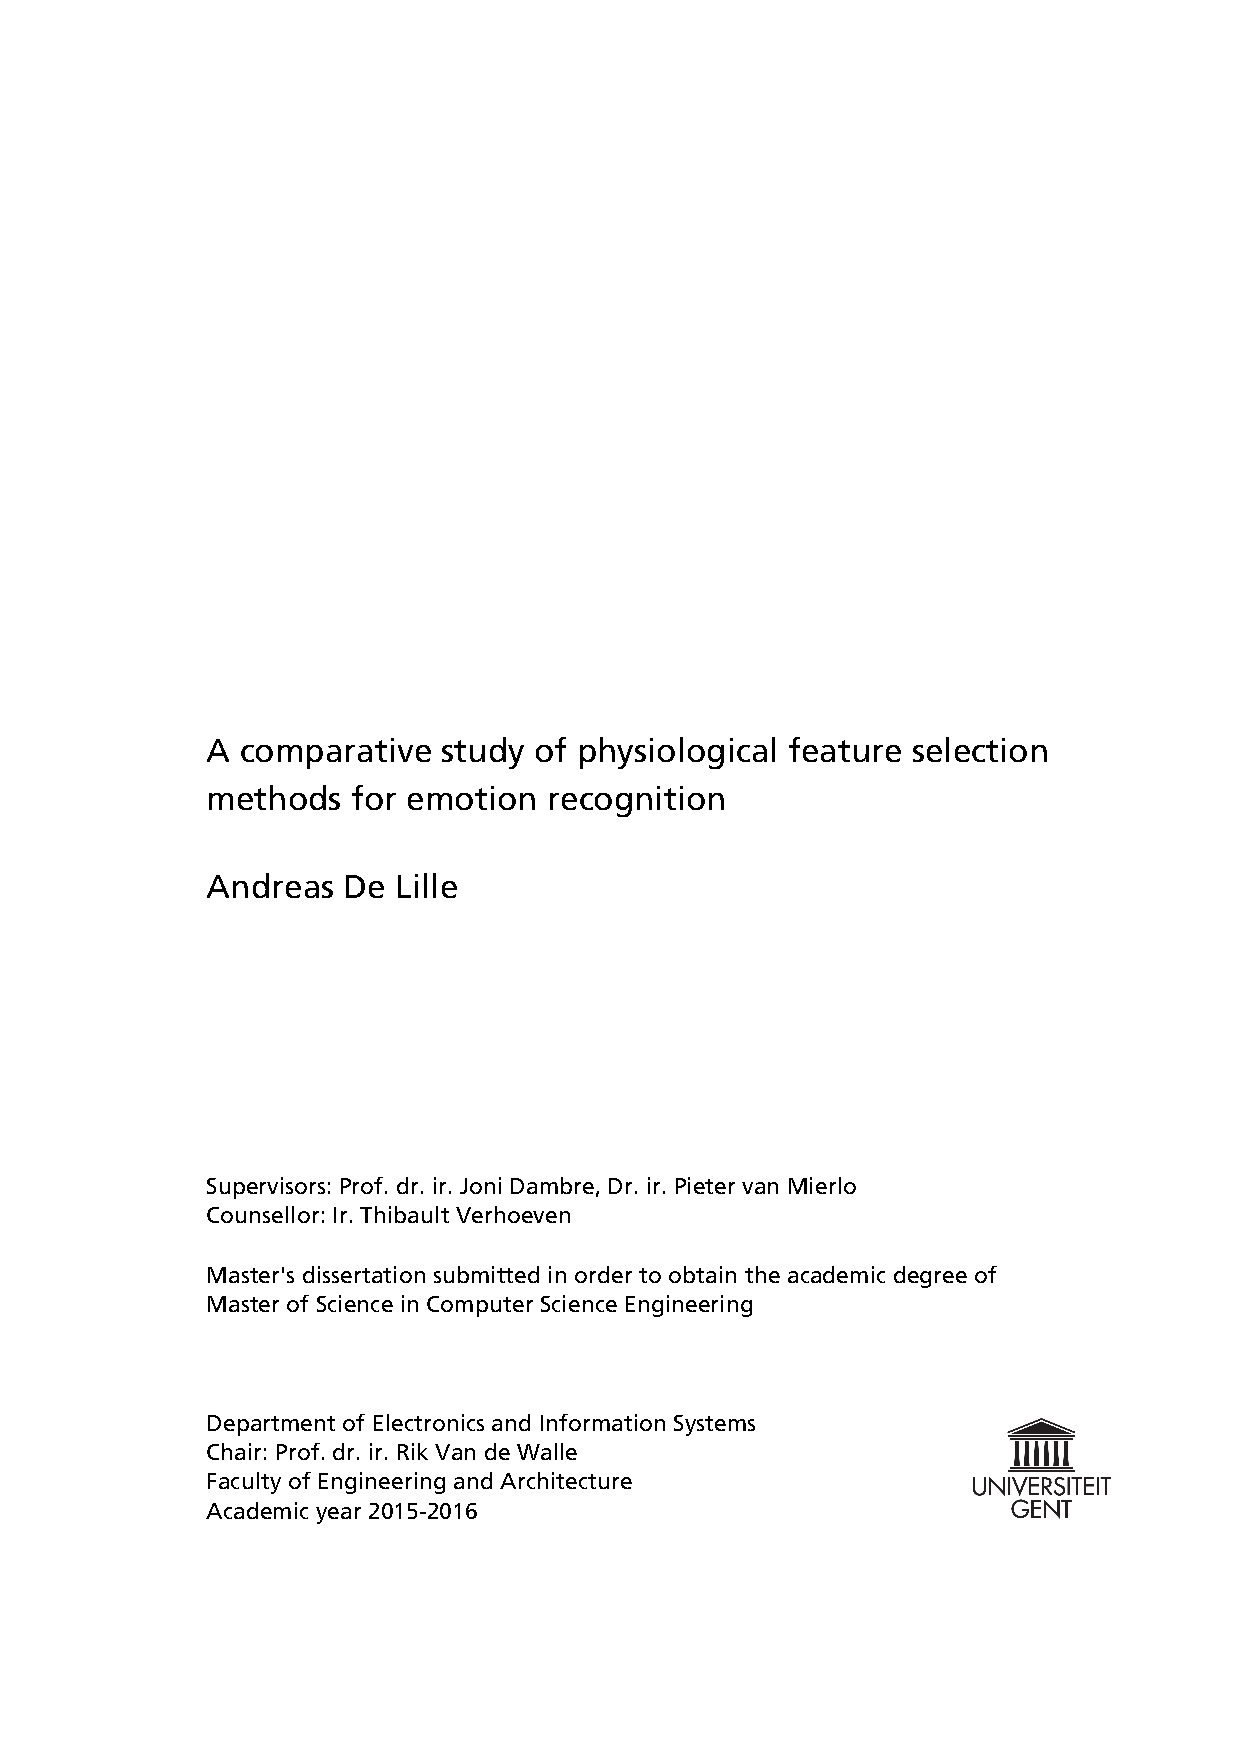
\includepdf[pages={1}, offset=75 - 75]{voorblad.pdf}
\afterpage{\blankpage} \clearpage
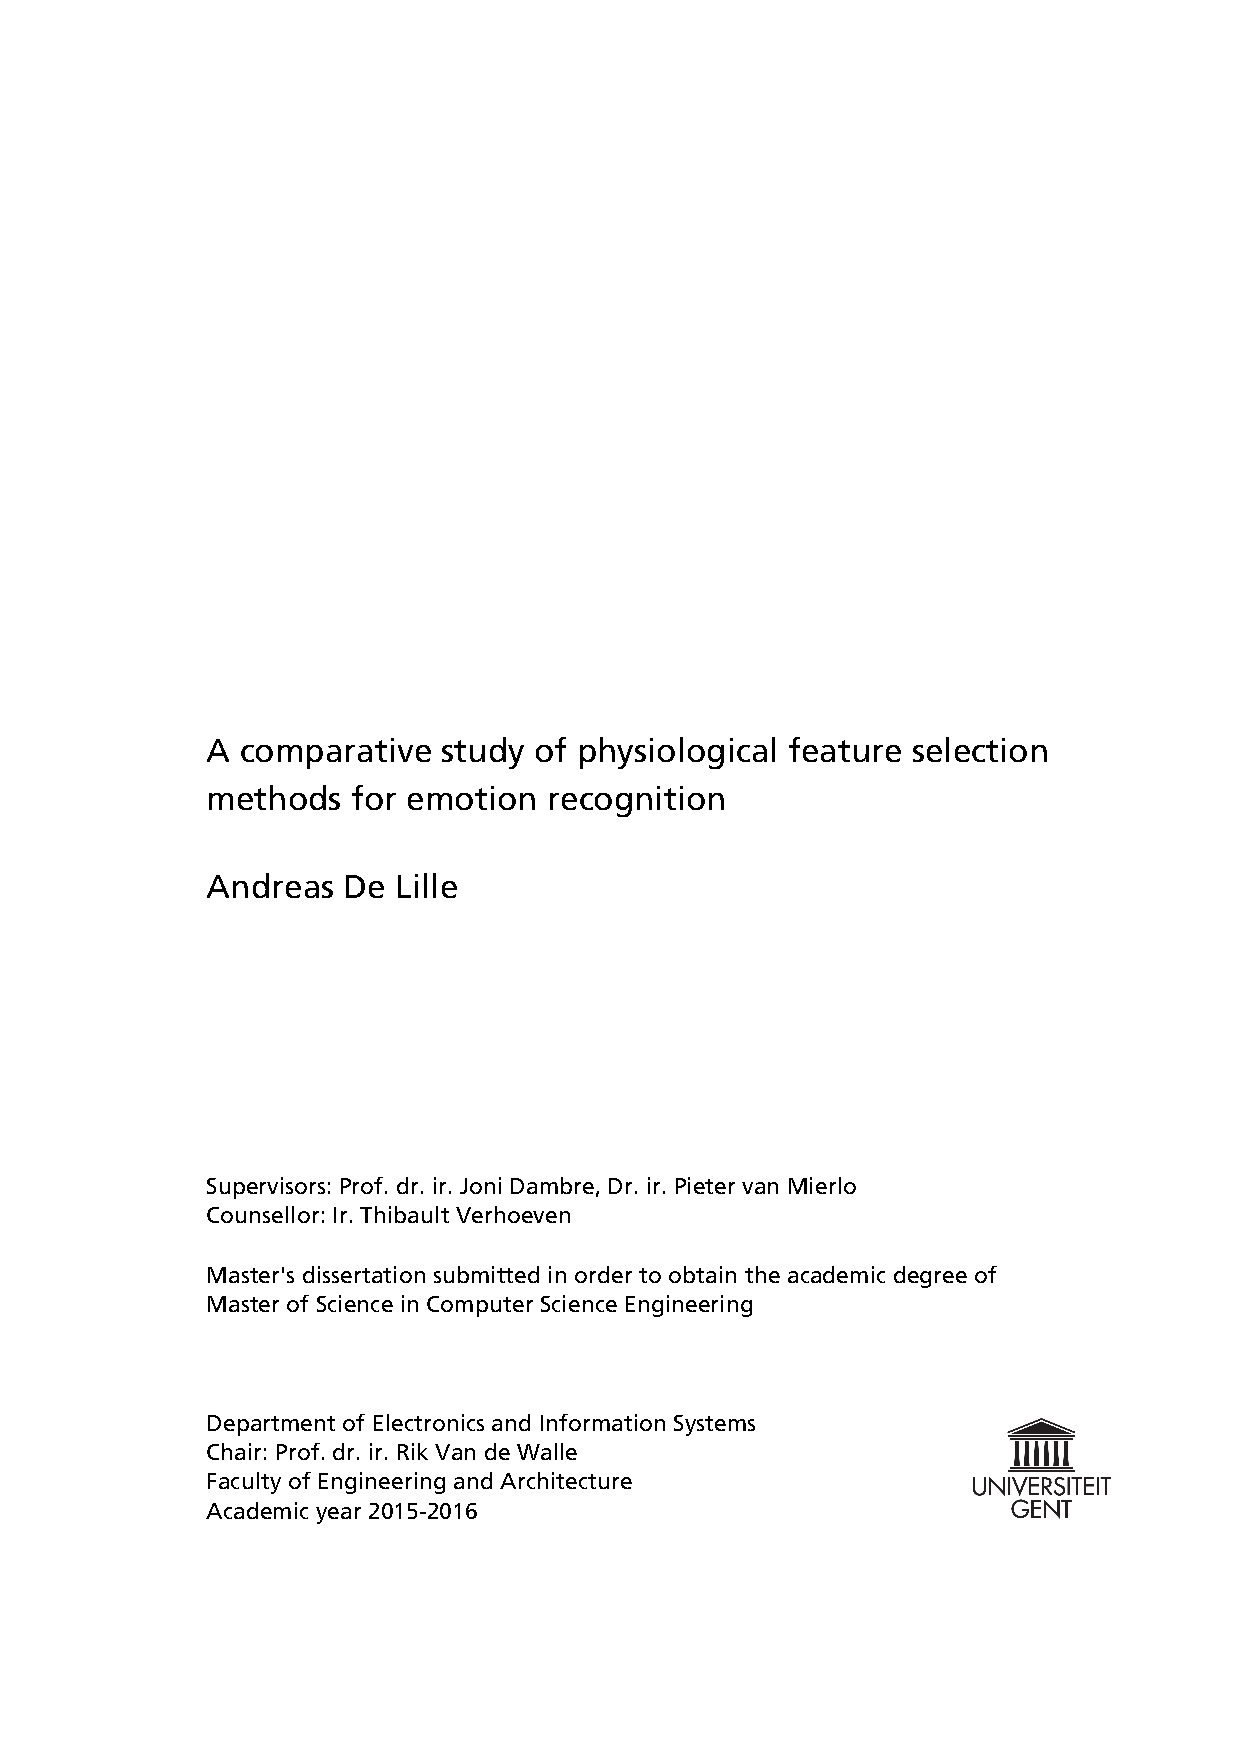
\includepdf[pages={1}, offset=75 - 75]{voorblad.pdf}

% geen paginanummering tot we aan de inhoudsopgave komen
\pagestyle{empty}
\renewcommand{\thepage}{\roman{page}}

% voorwoord met dankwoord en toelating tot bruikleen (ondertekend)
%  Voorwoord (dankwoord) en toelating tot bruikleen

\newpage

\noindent \textbf{\huge Voorwoord}

\vspace{1.5cm}

\noindent
Hier komt wat tekst.

\addvspace{4cm}

\noindent David De Reu, mei 2002\newpage

\noindent \textbf{\huge Toelating tot bruikleen}

\vspace{1.5cm}

\noindent
``De auteur geeft de toelating deze scriptie voor consultatie beschikbaar
te stellen en delen van de scriptie te kopi\"eren voor persoonlijk
gebruik.\\
Elk ander gebruik valt onder de beperkingen van het auteursrecht,
in het bijzonder met betrekking tot de verplichting de bron uitdrukkelijk
te vermelden bij het aanhalen van resultaten uit deze scriptie.''

\addvspace{4cm}

\noindent David De Reu, mei 2002


% abstract
%  Overzichtsbladzijde met samenvatting

\newpage
\addcontentsline{toc}{chapter}{Overview}
{
\setlength{\baselineskip}{14pt}
\setlength{\parindent}{0pt}
\setlength{\parskip}{8pt}

\begin{center}

\textbf{\huge
A Comparative Study of \\
Physiological Feature Selection Methods \\
for Emotion Recognition\\
}

by

Andreas DE LILLE

\end{center}

Supervisors: Prof.~J.~DAMBRE and Dr.~Ir.~P.~BUTENEERS \\
Counsellor: Ir.~T.~VERHOEVEN

Master's dissertation submitted in order to obtain the academic degree of\\
Master of Science in Computer Science Engineering

Department of Electronics and Information Systems\\
Chair: Prof. dr. ir. Rik Van de Walle\\
Faculty of Engineering and Architecture\\
Academic year 2015-2016\\



\section*{Summary}

An emerging field of research is the field of emotion recognition. Emotion can be observed in many ways, but the most reliable method is to use physiological signals.  This method uses machine learning to classify emotions based on characteristics or features extracted from the signals. To do so, good, reliable features are needed. This method compares a wide range of features and feature selection techniques to study the physiological responses triggered by emotion.

\section*{Keywords}

Emotion recognition, Physiological Signals, Machine Learning, Feature Selection

}

\newpage % strikt noodzakelijk om een header op deze blz. te vermijden


%extended abstract as pdf
\addcontentsline{toc}{chapter}{Extended Abstract}
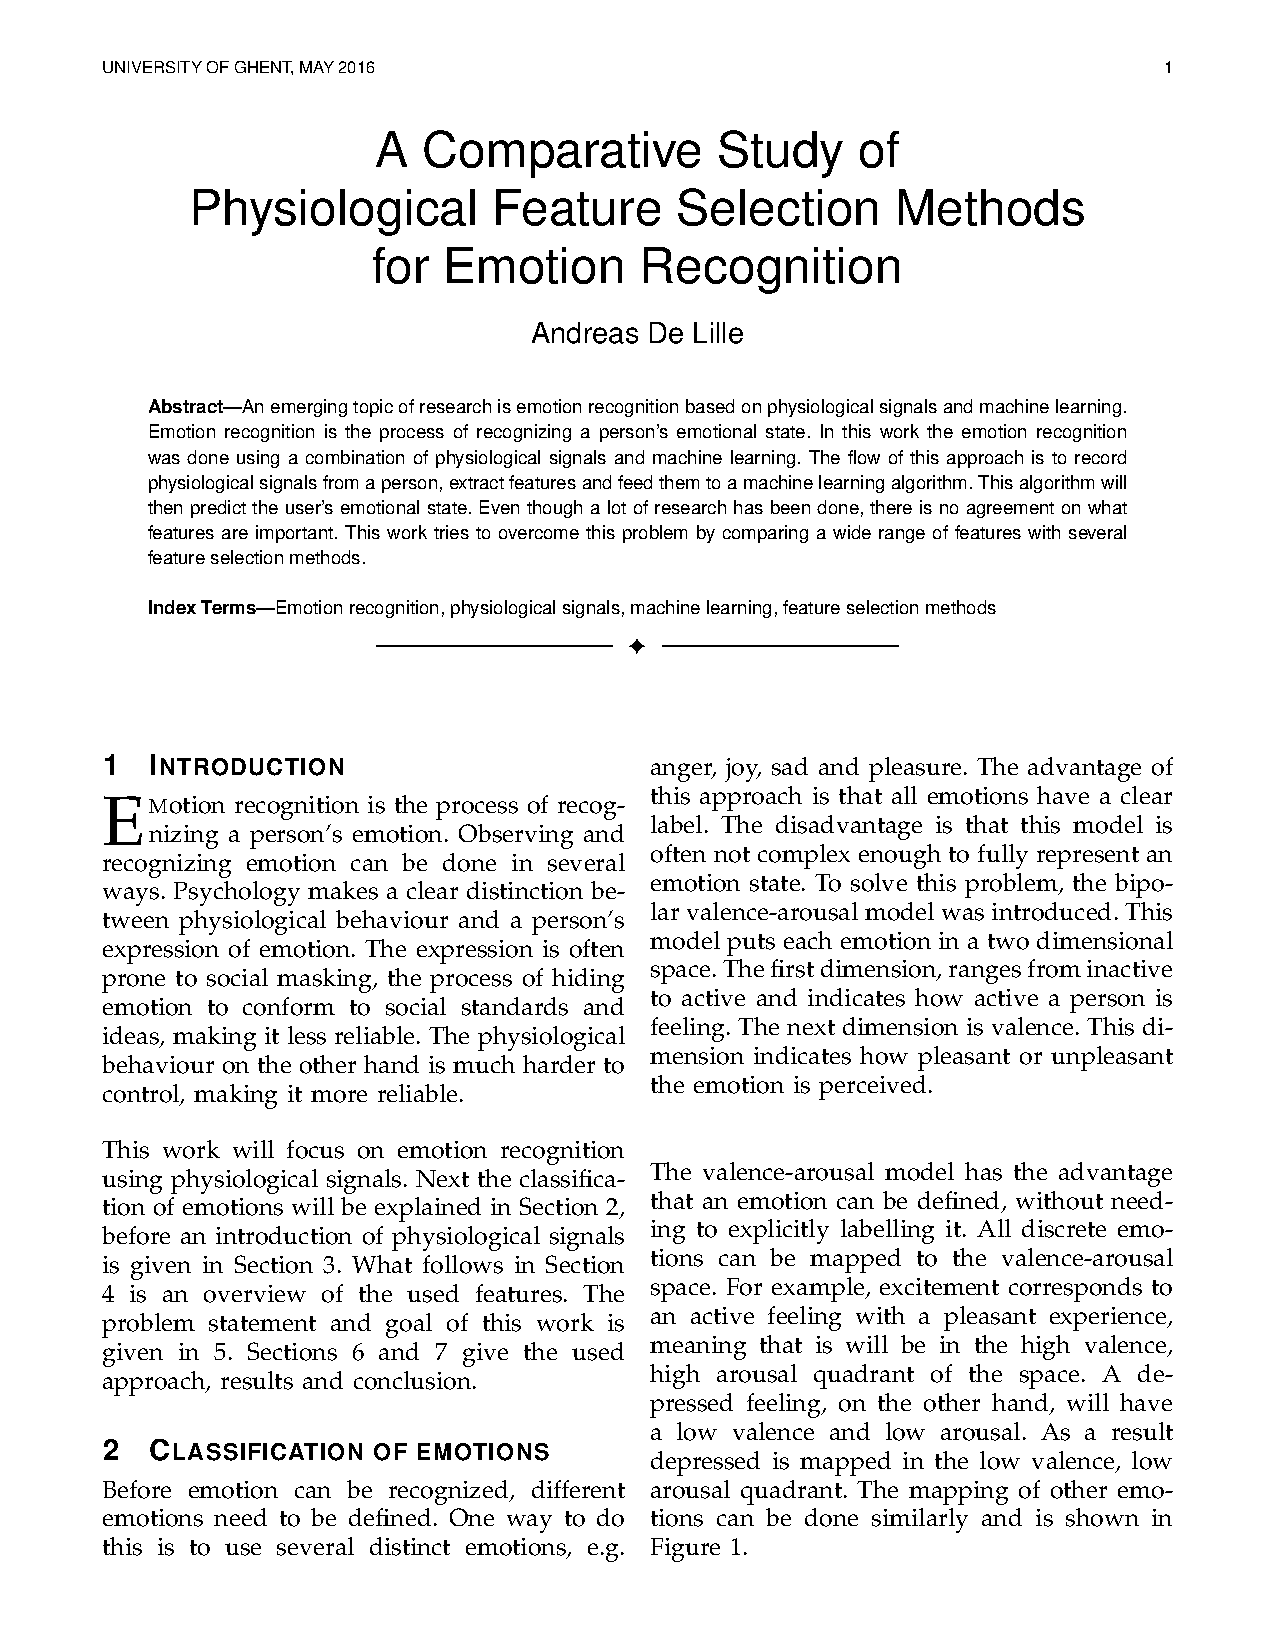
\includepdf[pages={1,2,3,4,5,6,7},offset=75 -75]{paper/bare_adv.pdf}

\pagestyle{fancy}
\frontmatter

\setcounter{page}{6}

% inhoudstafel
\tableofcontents
\addcontentsline{toc}{chapter}{Table of Contents}

% eventueel: lijst van figuren en tabellen
\listoffigures
\listoftables

%afkortingen
\printglossaries

% opmaak voor het eigenlijke boek; onderstaande lijnen
% weglaten als de eerste regel van een nieuwe alinea moet
% inspringen in plaats van extra tussenruimte
\setlength{\parindent}{0pt}
\setlength{\parskip}{0.5\baselineskip plus 0.5ex minus 0.2ex}
\setlength{\parskip}{1ex plus 0.5ex minus 0.2ex}

%\renewcommand{\thepage}{\arabic{page}}

% hoofdstukken
\mainmatter

% hier worden de hoofdstukken ingevoegd (\includes)
\chapter{Introduction}
{\samenvatting This chapters introduces the masterthesis. It starts by introducing the basic concepts of emotion recognition based on physiological signals, machine learning. Then it explains the problem statement and the goal of the thesis, followed by an overview of the next chapters.}

\section{Emotion recognition}

Human-to-machine communication, where humans communicate with machines or computer agents, is becoming more and more common\citep{hummaccom}. Fully understanding human communication is a complex problem. In addition to verbal communication, non-verbal communication is also used to exchange information\citep{EmotionRelativePower}. To better understand human-to-machine communication, more insight in the non-verbal communication is needed. Emotion recognition is becoming an increasingly important field as a result\citep{RealTimeEEGEmotion}.

\npar 

Emotion recognition is the proces of recognizing a subject's emotional state. In psychology a clear distinction between physiological behavior and the conscious experience of an emotion, called expression\cite{ExtendedPaper} is made. Expression consists of many parts, including facial expression, body language and voice concern\citep{EMSpeech}. Unlike expression, the physiological aspect of an emotion, e.g. heart rate, skin conductance and pupil dilation, is much harder to control. This makes emotion recognition based on physiological signals more robust to social masking\citep{PhytoEm}. Social masking is the process where an individual masks or hides their emotions to conform to social pressure. To really know one's emotions, it seems, one has to research the physiological aspect of the emotion.

\npar

\label{valarrdomspace}
Before emotions can be recognized, an objective class model describing different emotions is needed. A simple way of achieving this is using several discrete emotions, e.g. anger, joy, sad and pleasure. A more convienent model to classify emotions is the bipolar arousal-valence model\cite{ExtendedPaper,RealTimeEEGEmotion}, which places emotions in a two dimensional space. The main advantage of using a continuous multidimensional model, is that all emotions are modelled in its space, even when no particular discrete label can be used to define the current feeling. Figure \ref{ArousalValenceModel} shows the mapping of different emotions for this model. 

\npar

The valence-arousal model consists of two dimensions. Arousal indicates how active a person is and ranges from inactive/bored to active/excited. The valence indicates if the emotion is perceived as positive or negative. Even though arousal and valence describe emotions quite well, a third dimension, dominance, can also be added. This third dimension indicates how strong the emotional feeling was and ranges from a weak feeling to an empowered, overwhelming feeling. The dominance component can aid to filter out samples of strong feelings, since feelings with low dominance are less likely to show significant effects.

\mijnfiguur{width=0.45\textwidth}{ArousalValenceModel}{The arousal - valence model maps emotions in a two dimensional plane\citep{ValArrFig}}

\subsection{Physiological signals}

Now that the classification model is defined, the different physiological signals will be explained. As mentioned before, these signals are used to do automatic emotion recognition. Physiological signals can be divided in two subgroups: brain activity and other signals, e.g. heart rate, respiration rate, etc. Different technologies exist to record brain activity. The most convenient method is electroencephalography (EEG)\nomenclature{EEG}{Electroencephalography}, since it is a non-invasive method. Non-invasive methods, in contrast to invasive methods require no surgery. In case of EEG, they simply measure electrical activity using electrodes placed on the scalp.

\npar

Electrical activity in the brain is generated when an incoming signal arrives in a neuron. This triggers some sodium ions to move inside the cell, which in turn, causes a voltage rise\cite{ExtendedPaper}. When this increase in voltage reaches a threshold, an action potential is triggered in the form of a wave of electrical discharge that travels to neighbouring neurons. When this reaction occurs simultaneously in a lot of neurons, the change in electrical potential becomes significant enough, it is measured by the EEG surface electrodes. EEG can thus only capture synchronized activity of many, many neurons\cite{ExtendedPaper}. This explains why EEG signals have low spatial resolution capabilities. EEG measurements consist of electrical potentials of different channels, measured over time, like shown in Figure \ref{eegexample}.

\mijnfiguur{width=0.9\textwidth}{eegexample}{EEG measurements is a trace electrical potentials of different channels over time.\citep{EEGExampleFig}}

Signals originating from the cortex, close to the skull, are easier to measure, while signals originating deeper in the brain cannot be observed directly. Even for signals originating close to the cortex, EEG is far from precise as the bone between the the cortex and electrodes distorts the signal. Additionally, other artifacts like eye and muscle movement add a lot of noise to the signal. This explains why EEG signals are very noisy by nature. Noise removal techniques are therefor advised\citep{noiseRem}. Note that even though EEG data contains a lot of noise and has a low spatial resolution, it still provides significant insight into the electrical activity of the cortex while offering excellent temporal resolution\cite{GivenPaper}.

\npar

To ensure that experiments are replicable, standards for locations of electrodes have been developed. One of these systems is the 10/20 system, an internationally recognized method to describe the location of scalp electrodes\cite{TenTwentyManual}. The numbers 10 and 20 refer to the distances between the electrodes, which are either 10\% or 20\% of the total front-back or left-right distance of the scalp, this is depicted in Figure \ref{1020ElectrodePlacementSystem}. 

\mijnfiguur{width=0.8\textwidth}{1020ElectrodePlacementSystem}{The electrode placement of a 23 channel system\cite{1020Site}.}

Each site is identified with a letter that determines the lobe and a number that determines the hemisphere location.
\begin{itemize}
\item \textbf{F:} Frontal
\item \textbf{T:} Temporal
\item \textbf{C:} Central
\item \textbf{P:} Parietal
\item \textbf{O:} Occipital
\end{itemize}
Note that no central lobe exists; the C letter is only used for identification purposes. The letter z indicates that the electrode is placed on the central line. Even numbers are used for the right hemisphere, while odd numbers are used for the left hemisphere. Note that the 10/20 system does not require a fixed number of channels. Some experiments may use a different set of channels, but they all follow the same naming convention. In this work, a 32 channel EEG cap is used. The corresponding electrode locations are shown in Figure \ref{1020labels}

\mijnfiguur{width=0.7\textwidth}{1020labels}{Placement of the 32 electrodes in this thesis.}

In the frequency domain, brain waves are usually split up into different bands\cite{EmotionRelativePower,WavesSite}, with a different medical interpretation for each band. These wavebands \label{wavebands} are:
\begin{enumerate}
\item \textbf{Alpha:} 8-13Hz, indicate how relaxed and/or inactive the brain is.
\item \textbf{Beta:} 13-30HZ, indicate a more active and focused state of mind.
\item \textbf{Gamma:} 30-50Hz, relate to simultaneous processing of information from different brain areas.
\item \textbf{Delta:} 0-4hz, these waves are generated during dreamless sleep and meditation.
\item \textbf{Theta:} 4-8Hz, occurs during dreaming.
\end{enumerate}

\npar

Even though EEG is used in this thesis, alternative methods to measure brain activity exist. What follows is an overview of some of these techniques.
\begin{itemize}

\item Magnetoencephalography (MEG)\nomenclature{MEG}{magnetoencephalography} use magnetic fields to measure brain activity\citep{meg}. Since MEG is more prone to noise from external magnetic signals, i.e. the earth's magnetic field and electromagnetic communication, a magnetic shielded room is required, making this method very expensive and not mobile.

\item Functional magnetic resonance (fMRI) \nomenclature{fMRI}{Functional Magnetic Resonance}\citep{fMRI}: works by detecting changes in blood oxygenation and blood flow. An active area of the brain consumes more oxygen and has an increased blood flow.

\item Computed tomography (CT) \nomenclature{CT}{Computed Tomography}\citep{CT}: uses X-rays to create an image of the brain. 

\item Positron emission tomography (PET) \nomenclature{PET}{Positron Emission Tomography}\citep{PET}: this methods uses trace amounts of short-lived radioactive material. When this material undergoes decay, a positron is emitted that is picked up by a detector.

\item Near infrared spectroscopy (NIRS) \nomenclature{NIRS}{Near Infrared Spectroscopy}\citep{NIRS}: an optical technique to measure blood oxygenation in the brain. This technique works by shining light in the near infrared part of the spectrum through the skull and measuring how much remerging light is attenuated.

\end{itemize} 

In addition to brain activity, other physiological signals are also used in this work. The most known signal is the heart rate, which measures the number of contractions per minute. Respiration rate gives to number of breaths a human takes in one minute\citep{DEAP}. Another physiological signal is the galvanic skin response. The galvanic skin response measures the electrical characteristics of the skin\citep{GSR, DEAP}. In addition to the electrical characteristics, the temperature of the skin can also be measured. A plethysmograph is another physiological signal, that measures changes in volume within an organ\citep{DEAP}. A plethysmograph can be used to measure a subject's blood pressure and heart rate.

\section{Machine learning}
Machine learning is the missing link between the physiological signals and the emotion recognition. It is, in short, an input output model, that takes physiological signals and maps them to an emotional state. Machine learning is a very broad domain. As a result, this discussion will be limited to an introduction of the basic machine learning concepts with the focus on the application of machine learning and machine learning techniques used in this thesis. 

\npar

A possible definition for machine learning is: "the science of getting computers to act without being explicitly programmed"\citep{MLDef}. To do so, machine learning uses pattern recognition to find patterns or structure in the data. A simple example of machine learning is the Optical Character Recognition (OCR)\nomenclature{OCR}{Optical Character Recognition}, where a computer recognises characters in pictures\citep{OCR}. An example of OCR is shown in Figure \ref{OCR}.

\mijnfiguur{width=0.3\textwidth}{OCR}{In optical character recognition, a computer uses machine learning to find characters in an image\cite{OCRFigRef}.}

To further explain how machine learning works, have a look at the following example. Suppose one has a price list of houses that are for sale combined with their total area, shown in Table \ref{mlexampleTable}. Logic sense dictates us that a bigger house will have a higher price than a smaller house. The total area is a characteristic of the house that helps us in determining the price. In the context of machine learning, the characteristic 'total area', will be called a feature as the asking price of a house is correlated to the total area.

\begin{table}[H]
\centering
\begin{tabular}{ll}
\textbf{Area of the house ($m^{2}$)} & \textbf{Price ( x 1000 EUR)} \\
70                              & 312                          \\
73                              & 429                          \\
76                              & 174                          \\
79                              & 410                          \\
82                              & 334                          \\
$\vdots$                        & $\vdots$
\end{tabular}
\caption{total area of different houses and their corresponding asking prices.\label{mlexampleTable}}
\end{table}

One possible way of predicting the asking price of a house is machine learning. Machine learning works in several steps, first you train the machine learning algorithm with a list of asking prices and the corresponding area of the house. This process is called training or fitting and gives the machine learning component an idea to what price corresponds to a house with a certain area. Once trained, the algorithm's output will look like Figure \ref{mlexample}. The black dots represent the data points from Table\ref{mlexampleTable}. The blue line represents the predicted price for different area. The predicted price is simply defined by the total area of the house multiplied by some weight.

\mijnfiguur{width=0.9\textwidth}{mlexample}{The price of a house is determined by its total area.}

\clearpage

Even though, the blue line looks reasonable, there is sometimes a big difference between the predicted value and the actual value. This is due to the fact that the area of the house is only one feature that determines the price. Other features, like the number of bedrooms or the location of the house, were not taken into consideration. Adding additional features, gives more insight into the data, e.g. a house with 5 bedrooms is more expensive than a house with only 3 bedrooms. Having more features is thus likely to improve the performance of the machine learning algorithm.

\npar

There are many machine learning algorithms. One way to group these algorithms is to look at the produced output. In the asking price examples above, the output is a price, which is (more or less) a continuous value. Machine learning problems that require the output of a continuous value, are called regression problems\citep{prml}. In the OCR example above, a picture of a character is classified as a character. This means that OCR is a classification problem, as there are only a limited number of characters in an alphabet\citep{prml}.

\npar

Another way to group algorithms is based on their training data\citep{prml}. In the asking price examples above, the training data consists of labelled results. Labelled training data corresponds to data where the correct output (in this case the asking price) is given for each input (the area). This type of machine learning is referred to as supervised machine learning\citep{prml}. The alternative is unsupervised machine learning\citep{prml}. Unsupervised learning often results in finding groups of similar data points (clustering), without knowing the actual labels. Note that the combination of supervised and unsupervised data, known as semi-supervised learning, is also possible\citep{semiSup}. Imagine a dataset with 5000 webpages that need to be grouped into 10 distinct categories, e.g. science, nature, cooking, ... . Only 100 of the 5000 pages in the train set are labelled. An approach to solve this problem could be to first cluster the pages in similar groups using unsupervised learning. As soon as a group contains a single labelled page, all pages in the group can be labelled accordingly. This is possible because clustering returns groups of similar samples. Semi supervised learning has the advantage that one can also use unlabelled data, which is often easier and cheaper to obtain, unlike labelled data which is usually quite rare; if there was a fast and easy way to label the data then there would not be a need for machine learning.

\subsection{Over- and underfitting}

Over and underfitting is a common problem in many machine learning projects\citep{prml}. Suppose the example in Figure \ref{overunderfitting}, where one tries to find a good function to fit the given data points. Looking at the three proposed functions, one can easily see that the middle figure corresponds to the most logical generator function<\footnote{A generator function is a theoretical concept to describe the 'actual' function that generated the outputs.} of the red points.

\mijnfiguur{width=0.9\textwidth}{overunderfitting}{Overfitting versus underfitting\cite{overunderfittingFig}.}

\npar

The figure on the left corresponds to an underfit, where the proposed function is not able to capture sufficient detail of the points. The function is not complex enough to approach the generator function. As a result the best fit will always contain a relatively big error.

\npar

The function on the right corresponds to an overfit. The function fits or 'goes through' each point exactly, which will a very low error for these data points. However, one can see that the behaviour of the hypothesis function in between data points is not what one would expect. This is the result of using a too complex function to fit the data. As a results, all sample points are matched exactly, which results in a very low error for these points. However, the problems arise when the algorithm is test on unseen points. The algorithm will have a much higher error for those points. 

\npar 

Part of a good machine learning algorithm is finding the right tradeoff between overfitting and underfitting. In case of the aforementioned overfitting, it would be better to lower the performance of the algorithm on the sample datapoints, to gain performance on the 'unseen' datapoints. Different techniques exist to estimate how good an algorithm performs on unseen points. Often a part of the sample points is put in a test set that is neglected during training. After the algorithm is designed, the performance on the test set will indicate how well the algorithm generalises. It is only the performance of the test set that gives a fair estimation of the performance of a machine learning algorithm.

\subsection{Feature selection}
Feature selection is a technique that aims at selecting the features that perform well, while trying to remove irrelevant features\citep{rfPaper}. The advantages of having a smaller features set are twofold. First having fewer features, will lower the risk of overfitting\citep{rfPaper}. Second, knowing which features are important makes it possible for humans to interpret the machine learning model. In this thesis, knowing which features are relevant might help in gaining insight in the processing of emotion by the brain. 

\clearpage

There exist several approaches to do feature selection. The first one is to simple use a statistical metric and remove all features with low correlation to the output. Another approach is to look at the weights of a model. When a machine learning model gives a large weight to a feature, then that feature is considered more important than a feature with an assigned weight close to zero. Embedded methods also exist, they rely on the build in feature selection mechanisms of some machine learning algorithms. A more thorough  overview of the different feature selection techniques is given in Section \ref{FSSel}. 

\section{Problem statement}

A lot of different physiological features are reported in the literature. Unfortunately, the literature does not fully agree on a specific set of features nor does it agree on what EEG channels and/or frequency bands are most important for emotion recognition. The features that are reported in different studies are often quite different, as you can see in Table \ref{diffFeat} below.

\begin{table}[H]
\centering
\begin{tabular}{ll}
\textbf{study} & \textbf{features used}                         \\
\citep{ref4}     & Alpha and beta power                           \\
\citep{ref7}     & PSD and asymmetry features                     \\
\citep{ref8}     & PSD                                            \\
\citep{ref6}     & discrete wavelet transform of alpha, beta and gamma band \\
\citep{ExtendedPaper}	&	alpha/beta ratio, Fpz beta and alpha band power \\
\citep{killyPaper} & PSD, RCAU, DCAU, DASM, RASM, DE \\
\end{tabular}
\caption{Six different papers on emotion recognition, six different feature sets\label{diffFeat}.}
\end{table}

\npar

Another related problem with physiological signals is that they are very personal by nature. Features that work well for one person might not work well for another person\citep{DEAP}. Finding a set of features that works well for all persons is hard, but it might make the system more robust against personal differences. 

\npar

The last problem is that is hard to compare the performance of different physiological feature studies, as they do not share the same dataset.

\section{Goal of the thesis}
The first goal is finding relevant features for emotion recognition in a person specific setting. This is already quite challenging as there are fuzzy boundaries and individual variation of emotion\citep{emorecoghard}. To do so, the output of different feature selection methods is compared. In a successful scenario, good features are found. These features could be used by a machine learning algorithm to accurately predict the emotions of one person. Some attention will also be spend on comparing non-EEG and EEG features to see which whether it is useful or not to include EEG and/or non-EEG signals in the emotion recognition.

\clearpage

The second goal is finding features for emotion recognition in a cross-person setting. In this setting features should generalise well across different persons, thus the algorithm should be able to recognize emotions from unseen persons. The comparison for non-EEG and EEG features will also be done here. Emotion recognition is harder in a cross-person setting, since physiological signals are very personal\citep{DEAP}.

\npar 

Both goals are tackled by comparing a large range of different feature selection methods combined with a huge feature set. Additionally, the accuracy on the DEAP, a dataset designed to compare different emotion recognition studies\citep{DEAP} will be reported. This will ensure that the results obtained in this thesis can serve as a benchmark for future research. This is important as performance of emotion recognition algorithms based on physiological signals often varies a lot for different datasets\citep{PhytoEm}.

\npar 

The contents of this thesis are as follows. The next chapter gives an overview of the dataset, features and feature selection methods that are used in this thesis. It also gives an overview of similar state of the art emotion recognition studies.
 
\npar
Chapter 3 and 4 give an overview of the obtained results for person specific and cross-person emotion recognition respectively. Chapter 5 gives the conclusion of this work. Chapter 6 gives an overview of future research that is possible.
\chapter{Methods}
{\samenvatting This chapter starts by giving an overview of the features found in literature for emotion recognition. Then an overview of some emotion recognition studies is given. The chapter ends by explaining the different feature selection methods.} %TODO 

\subsection{Dataset}
One of the most used datasets in the context of emotion recognition is the Dataset for Emotion Analysis using Physiological Signals (DEAP)\nomenclature{DEAP}{Dataset for Emotion Analysis using Physiological Signals}\cite{DEAP}. This dataset consists of several parts, the first part is a rating of 120 music videos by 14 - 16 persons. Each video is rated for valence, arousal and dominance on a scale ranging from 1 to 9 using self-assessment manikins (see later). This part of the dataset is not used during this thesis, because it contains no recordings of physiological signals.

\npar

The next part of the dataset is the physiological experiment that contains emotional reactions of 32 subjects. The emotional reactions were triggered using music video excerpts; each subject watched 40 one-minute videos, while several physiological signals were recorded. These physiological signals consist of 32 channel 512Hz EEG and peripheral physiological signals. More concretely, this dataset contains following signals:
\begin{table}[H]
\centering
\begin{tabular}{l|ll|l|ll}
\textbf{Channel} & \textbf{Name} & \textbf{Category} & \textbf{Channel} & \textbf{Name}    & \textbf{Category} \\ \hline
\textbf{1}       & Fp1           & EEG               & \textbf{21}      & F8               & EEG               \\
\textbf{2}       & AF3           & EEG               & \textbf{22}      & FC6              & EEG               \\
\textbf{3}       & F3            & EEG               & \textbf{23}      & FC2              & EEG               \\
\textbf{4}       & F7            & EEG               & \textbf{24}      & Cz               & EEG               \\
\textbf{5}       & FC5           & EEG               & \textbf{25}      & C4               & EEG               \\
\textbf{6}       & FC1           & EEG               & \textbf{26}      & T8               & EEG               \\
\textbf{7}       & C3            & EEG               & \textbf{27}      & CP6              & EEG               \\
\textbf{8}       & T7            & EEG               & \textbf{28}      & CP2              & EEG               \\
\textbf{9}       & CP5           & EEG               & \textbf{29}      & P4               & EEG               \\
\textbf{10}      & CP1           & EEG               & \textbf{30}      & P8               & EEG               \\
\textbf{11}      & P3            & EEG               & \textbf{31}      & PO4              & EEG               \\
\textbf{12}      & P7            & EEG               & \textbf{32}      & O2               & EEG               \\
\textbf{13}      & PO3           & EEG               & \textbf{33}      & hEOG             & non-EEG           \\
\textbf{14}      & O1            & EEG               & \textbf{34}      & vEOG             & non-EEG           \\
\textbf{15}      & Oz            & EEG               & \textbf{35}      & zEMG             & non-EEG           \\
\textbf{16}      & Pz            & EEG               & \textbf{36}      & tEMG             & non-EEG           \\
\textbf{17}      & Fp2           & EEG               & \textbf{37}      & GSR              & non-EEG           \\
\textbf{18}      & AF4           & EEG               & \textbf{38}      & respiration belt & non-EEG           \\
\textbf{19}      & Fz            & EEG               & \textbf{39}      & plethysmograph   & non-EEG           \\
\textbf{20}      & F4            & EEG               & \textbf{40}      & temperature      & non-EEG          
\end{tabular}
\caption{The available signals in the DEAP dataset\label{DEAPSignals}.}
\end{table}

\npar

There also exists a preprocessed version of the physiological experiment database, where the EEG recordings were downsampled to 128Hz and noise and EOG artifact removal was performed. Additionally most muscle and eye artifacts have a frequency around 1.2Hz. Artifacts caused by nearby power lines, have a frequency around 50Hz\cite{ExtendedPaper}. A bandpass filter was usually applied to filter out frequencies below 4Hz and above 40-45Hz.

\npar

Additionally facial video for 22 of the 32 subjects was recorded, so research in facial expressions is also possible with this dataset. These videos are also rated on 4 scales: arousal, valence, dominance and liking. The liking component indicates how much the person liked the video excerpt and should not be confused with the valence component; it inquires information about the participants' tastes, not their feelings, i.e. a person can like a video that triggers angry or sad emotions. However strong correlations were observed\citep{DEAP}. The liking rates are neglected, since they are not part of the emotion space.

\npar

For assessment of these scales, the self-assessment manikins (SAM)\nomenclature{SAM}{self-assessment manikins}, were used\cite{DEAP}. SAM visualizes the valence, arousal and dominance scales with pictures. Each picture corresponds to a discrete value. The user can click anywhere in between the different figures, which makes the scales continuous. All dimensions are given by a continuous value between 1 and 9. In this thesis, a preprocessing step scaled and translated these values to ensure they range between 0 and 1, a more convenient interval.

\npar

The used SAM figures are shown in Figure \ref{SAM}. The first row gives the valence scale, ranging from sad to happy. The second row shows the arousal scale, ranging from bored to excited. The last row represents the different dominance levels. The left figure represents a submissive emotion, while the right figure corresponds with a dominant feeling.

\mijnfiguur{width=0.5\textwidth}{SAM}{The images used for the SAM\cite{DEAP}.}

\section{Features}
\label{featuresExplained}
Machine learning algorithms require good features to perform well\footnote{Note that there are some exceptions, for instance some types neural networks are capable of 'designing' their own features\citep{nnfeat}. But these algorithms were not used in this thesis.}. In the context of this thesis, good features should be correlated with the subject's emotional state. Two categories of features are observed in this work: EEG features and non-EEG features. Both categories are covered in the following sections.

\subsection{EEG-features}
EEG features are extracted from the electroencephalography measurements from the subject's scalp. From these signals a lot of different signals can be extracted. The power spectral density (PSD) \nomenclature{PSD}{Power Spectral Density} of a signal gives the distribution of the signal's energy in the frequency domain. By calculating the spectral density for different frequency bands of the signal, one can determine how much power of each frequency band is in the signal.

\npar

Differential entropy (DE)\nomenclature{DE}{Differential Entropy} is defined as follows \citep{killyPaper} \\
\begin{center}
$DE_{channel} = - \int_{-\infty}^{\infty} \frac{1}{\sqrt{2\pi\sigma^2}} exp(\frac{(x-\mu)^2}{2\sigma^2}) log(\frac{1}{\sqrt{2\pi\sigma^2}}) exp(\frac{(x-\mu)^2}{2\sigma^2})dx$
\end{center}
According to \citep{diffEnt}, the differential entropy of a certain band is equivalent to the logarithmic power spectral density for a fixed length EEG sequence, which simplifies the calculations significantly.
\begin{center}
$DE_{channel} = log(PSD_{channel})$
\end{center}

\npar

The most used feature for valence recognition is the frontal asymmetry of the alpha power\cite{GivenPaper}. The right hemisphere is generally speaking, more active during negative emotion than the left hemisphere which is in turn more active during positive emotions\cite{RealTimeEEGEmotion,EEGDatasets,killyPaper}. The asymmetry can be calculated in different ways. First, one can calculate the differential asymmetry (DASM) \nomenclature{DASM}{Differential Asymmetry}, where the left alpha power is subtracted from the right alpha power.

\begin{center}
$DASM = DE_{left} - DE_{right}$
\end{center}

Another way to measure the asymmetry is by division. The Rational Asymmetry (RASM) \nomenclature{RASM}{Rational Asymmetry} does exactly this and is given by: \\

\begin{center}
$RASM = \frac{DE_{left}}{DE_{right}}$
\end{center}

With $DE_{left}$ and $DE_{right}$ being the left and right differential entropy respectively. Another reported feature in literature is the caudality, or the asymmetry in fronto-posterior direction\cite{caudality}, meaning the difference in power between the front and the back of the scalp. This can again be calculated in two ways. The first method is the differential Caudality (DCAU) \nomenclature{DCAU}{Differential Caudality}, defined as: \\

\begin{center}
$DCAU = DE_{front} - DE_{post}$
\end{center}

The second method to determine the Caudality is the Rational Caudality (RCAU) \nomenclature{RCAU}{Rational Caudality}, which is defined as:

\begin{center}
$RCAU = \frac{DE_{front}}{DE_{post}}$
\end{center}

With $DE_{front}$ and $DE_{post}$ being the frontal and posterior power respectively. Arousal is usually determined, by looking at the different frequency bands\citep{ExtendedPaper}. Each frequency and has their own medical interpretation, see \ref{wavebands}. Alpha power corresponds to a more relaxed brain, while Beta power corresponds to a more active brain. The alpha / beta ratio therefore seems a good indicator for the arousal state of a person.

\npar

The Alpha/ Beta ratio is limited to comparing two frequency bands. Other frequently used features are fractions of PSD. The fractions of frequency band power is determined for a channel, given by:

\begin{center}
$frac_{band,channel} = \frac{power_{band,channel}}{power_{total,channel}}$
\end{center}

These fractions give insight in the distributions of wavebands at different channel locations.

\subsection{non-EEG features}
The aforementioned EEG features are just one class of physiological features, the DEAP dataset contains several non-EEG, physiological measurements\citep{DEAP}. For each of these measurements the average, standard deviation, variation, median, minimum and maximum are calculated.

\npar

The Galvanic Skin Response \nomenclature{GSR}{Galvanic Skin Response} uses two electrodes on the middle and index finger of the subjects left hand to measure the skin resistance. It has been reported that the mean value of the GSR is related to the level of arousal\citep{GSR, DEAP}.

\npar

The respiration belt (RSP)\nomenclature{RSP}{Respiration Belt}, indicates the user's respiration rate. Slow respiration is linked to relaxation (low arousal), while fast and irregular respiration patterns corresponds to anger or fear, both emotions with low valence and high arousal\citep{DEAP}.

\npar

A plethysmograph is a measurement of the volume of blood in the subject's left thumb. This can be use to determine the blood pressure. Blood pressure offers valuable insight into the emotional state of a person as it correlates with emotion; stress is known to increase blood pressure\citep{DEAP}.

\npar

The heart rate is not directly available in the DEAP dataset, but can be extracted from the plethysmograph, by looking at local minima and maxima\citep{DEAP}. This is clearly visible when looking at the plethysmograph's output, shown in Figure \ref{before}.

\mijnfiguur{width=0.9\textwidth}{before}{The plethysmograph before smoothing.}

The heart rate extraction is done in two steps. First the plethysmograph signal is smoothed, by filtering out the high frequency components to avoid noise being selected as a local optima. In the second stage the local optima are located, this is shown in Figure \ref{extrema}

\mijnfiguur{width=0.9\textwidth}{extrema}{The local optima in the plethysmograph.}

\npar

The combination of a local minimum and maximum correspond to a heart beat\citep{DEAP}. Therefore, the time between two consecutive local minima or maxima correspond to the time between two heart beats, known as the interbeat interval. Getting the average heart rate from the interbeat interval is straight forward. Lastly, the skin temperature of the subject is also available.

\subsection{Overview}

The following table gives an overview of the different features and their amount. The 32 EEG channels can be found in Table \ref{DEAPSignals}. There are 6 frequency bands: Alpha, Beta, Gamma, Delta, Theta and All. All refers to taking the total power of a channel. Note that the fractions only have 5 frequency bands, as the percentage of all power would always be 100$\%$. 

\begin{table}[]
\centering
\begin{tabular}{lllll}
\textbf{name}           & \textbf{type} & \textbf{number of channels}   & number of frequency bands & total number \\
\textbf{PSD}            & eeg           & 32                            & 6                         & 192          \\
\textbf{DE}             & eeg           & 32                            & 6                         & 192          \\
\textbf{DASM}           & eeg           & 13                            & 6                         & 78           \\
\textbf{RASM}           & eeg           & 13                            & 6                         & 78           \\
\textbf{DCAU}           & eeg           & 11                            & 6                         & 66           \\
\textbf{RCAU}           & \textbf{eeg}  & 11                            & 6                         & 66           \\
\textbf{Frac}           & eeg           & 32                            & 5                         & 160          \\
\textbf{Alpha / Beta}   & eeg           & 32                            & 1                         & 32           \\
Total                   &               &                               &                           & 864          \\
                        &               &                               &                           &              \\
\textbf{name}           & \textbf{type} & \textbf{number of statistics} &                           &              \\
\textbf{HR}             & non-eeg       & 6                             &                           &              \\
\textbf{plethysmograph} & non-eeg       & 6                             &                           &              \\
\textbf{GSR}            & non-eeg       & 6                             &                           &              \\
\textbf{ST}             & non-eeg       & 6                             &                           &              \\
\textbf{RSP}            & non-eeg       & 6                             &                           &              \\
\textbf{Total}          &               & 30                            &                           &              \\
                        &               &                               &                           &              \\
\textbf{Overall Total}  & \textbf{894}  &                               &                           &             
\end{tabular}
\caption{An overview of the different features that were compared in this thesis.\label{featOverviewTable}}
\end{table}

The feature set has a size of 894, which is huge considering that there are only 40 samples for each person. Using this many features in combination with the low sample count, will quickly result in overfitting\citep{prml}. To solve this problem, one can either increase the number of samples or decrease the number of features. Increasing the number of samples is hard. EEG data requires several recordings of subjects that need to spend the right amount of time. Reducing the feature set in size is another possibility. Two methods exists, dimension reduction and feature selection. Dimension reduction methods create combinations of features, while feature selection methods select a subset of the features. In case of feature selection, bad features are, in contrast to dimension reduction methods, neglected completely. %TODO ref

\npar

This is even more problematic in cross-subject emotion recognition. It is not possible to simply take a limited subset of features, since physiological signals are very personal by nature \citep{DEAP}. Selecting features that work for one person, might not work well on different persons.


\section{State of the art}
This section will give a overview of similar studies and their conclusions. Some of these studies also did some research on cross-subject emotion recognition. Since emotion recognition is still in its infancy\citep{emorecoghard} and subject independent features are hard to find \citep{DEAP}. Research is more focussed on person specific emotion recognition.

\subsection{DEAP method}
The first method of emotion recognition is the DEAP method, described in the DEAP paper\citep{DEAP}, the paper that introduces the DEAP dataset used in this thesis. The research found that Valence shows the strongest correlations with the EEG signals. Additionally the study found correlations in all frequency bands, with an increase in power for the lower range wavebands for an increase in valence. These effects occur in the occipital regions of the brain, above the visual cortices, which might indicate that the subject is focussing on a pleasurable sound. A central decrease in beta power was observed together with a occipital and right temporal increase in power for positive emotions. The research conclude that these observed correlations concur with other neurological studies, but that the absolute value of the correlations are seldom bigger than $0.1$ for a cross person setting, which indicates that cross person emotion recognition is a non trivial problem. The absolute values of the person specific correlations were around $0.5$.

\npar

The DEAP paper also presents their own classification method for person specific emotion classification. They start by performing feature selection using the Fisher's linear discriminant for feature selection. The Fisher's linear discriminant is defined as:

\begin{center}
$J(f) = \frac{|\mu_1 - \mu_2|}{\sigma_1^2 + \sigma_2^2}$ \
\end{center}

With $\mu$ and $\sigma$ being the mean and standard deviation of feature f. The Fisher's discriminant was calculated for each feature, before a threshold of 0.3 was applied to filter out irrelevant features. The used classifier was a Naive Bayes classifier, which assumes independence of features. The Naive Bayes classifier is a simple classifier that uses the following equation:

\begin{center}
$G(f_1, ..., f_n) = argmax_c p(C=c) \prod\limits_{i=1}^n p(F_i=f_i|C=c)$ \\
\end{center}

With F being the set of features and C the classes. $p(F_i=f_i|C=c)$ is estimated by assuming Gaussian distributions of features and modelling these from the training set.

\subsection{Stable emotion recognition over time}

In \citep{killyPaper}, research is done to find EEG patterns for emotion recognition that are stable over time. EEG patterns are not only subject dependent, they are also dependent on the subjects mood and thus might vary in time. The paper starts by researching different EEG features: PSD, DE, DASM, RASM, DCAU, RCAU, these features are explained in \ref{featuresExplained} and are tested on the DEAP dataset. Afterwards, they develop a new dataset, where subjects have repeated trial sessions with some time in between.

\npar

Their machine learning set-up is as follows, first they perform feature extraction of the aforementioned features. Then feature smoothing is done using a Linear Dynamic system (LDS) \nomenclature{LDS}{Linear Dynamic System}, that can be expressed by:
\begin{center}
$x_t = z_t + w_t$\\
$z_t = Az_{t-1} + v_t$
\end{center}
$x_t$ denotes the observed variables or features, while $z_t$ denotes the hidden emotion variables. $A$ is a transformation matrix and $w_t$ is Gaussian noise. The need for a linear dynamic system is supported by the assumption that emotion change gradually over time. The LDS filters out components that are not associated with emotional states.

\npar

The list of features at this point is too big and may contain uncorrelated features that might lead to performance degradation of the classifier. Two methods for this are compared, principal component analysis (PCA) and minimal redundancy maximal relevance (MRMR)\nomenclature{MRMR}{Minimal Redundancy Maximal Relevance}. 

\npar

PCA uses an orthogonal transformation to create a lower dimensional feature space starting from the original higher dimensional feature space. It does so by minimizing the loss of information, i.e. the principal component should have the largest possible variance. 

\npar

PCA cannot preserve original domain information like channel and frequency, therefore the paper also uses the MRMR method. MRMR uses mutual information in combination with maximal dependency criterion and minimal redundancy. The algorithm starts by searching features satisfying:

\begin{center}
$max D(S,c), D=\frac{1}{|S|} {\displaystyle \sum_{x_d \in S}} I(x_d;c)$
\end{center}

Where S is the feature subset to select. When two features are highly correlated, the maximal dependency is not likely to change when one of the correlated features is removed. This is expressed by the minimal redundancy condition.

\begin{center}
$min R(S), R = \frac{1}{|S|^2} {\displaystyle \sum_{x_{di}, x_{dj} \in S}} I(x_{di},x_{dj})$
\end{center}

The two conditions are then combined to from the Maximal Relevance Minimum Redundancy, which can be expressed as:

\begin{center}
$max \varphi(D,R), \varphi=D-R$
\end{center}
Note that incremental search methods exists and are often used in practice. After performing the dimensionality reduction, the samples from the DEAP data set are classified in high / low valence and high/low arousal, giving a total of four classes. All values close to the separation border are removed from the training data, as they might confuse the classifier. 

\npar 

For the classification, three conventional and one newly developed pattern classifiers were compared. k-nearest neighbors (KNN) \nomenclature{KNN}{k-nearest neightbors}, logistic regression (LR)\nomenclature{LR}{Logistic Regression}, Support Vector Machines (SVM) and Graph regularized Extreme Learning Machine (GELM) \nomenclature{GELM}{Graph regularized Extreme Learning Machine}. 

\npar

Extreme Learning Machine (ELM) \nomenclature{ELM}{Extreme Learning Machine} is a single layer feed forward neural network\citep{ELMpaper}. GELM is based on the idea that similar shapes should have similar properties and obtains better results for face recognition \citep{GELMpaper} and as the paper concludes, also for emotion classification.

\npar

The study found then performed a study on the different features and concluded that DE features are the most suitable EEG features, followed by the asymmetry features (RASM, DASM, DCAU and RCAU). The LDS smoothing was also found to be the better feature smoothing method. 

\subsection{EEG-based emotion recognition in music listening}

This study\citep{emorecoghard} uses EEG features to recognize 4 different discrete emotions (joy, anger, sadness, pleasure) induced by music. They compared four different feature sets on 6 different wavebands: RASM and DASM of 12 channelpairs, raw PSD of the 24 channels and PSD of 30 channels (including 6 midline channels). The compared set of wavebands consists of: alpha, beta, gamma, delta, tetha and all wavebands. These features were fed to two different classifiers, one Multilayer perceptron (MLP) \nomenclature{MLP}{Multilayer Perceptron} and an SVM. 

\npar

Their main results were that the DASM features worked better that the RASM features and even better than using the corresponding 24 PSD features. They also did research to person independent EEG features and found that their accuracy remained consistent. Note that while these results sound promising, they were unfortunately not performed on the DEAP dataset; performance of emotion recognition algorithms is known to vary a lot between datasets\citep{PhytoEm}.

\subsection{Comparing selected methods for feature extraction and classification}

The paper\citep{PhytoEm} classifies four distinct emotions (joy, anger, sadness and pleasure) triggered by songs that were selected for each subject. The songs were selected by the subject himself, to help him in triggering memories that trigger the desired emotions. The four emotions are mapped in the valence-arousal model. The used features were typical statistical values of physiological signals (Skin Conductivity (SC)\nomenclature{SC}{Skin conductivity}, Electrocardiogram (ECG), Electromygraphy (EMG) and Respiration rate (RSP). They compared several techniques: Analysis of Variance (ANOVA) \nomenclature{ANOVA}{Analysis of Variance} where the best d features were taken. Sequential forward selection (SFS) \nomenclature{SFS}{Sequential Forward Selection}, where the algorithm starts with an empty feature set and then introduces a new feature in each iteration. Sequential backward selection (SBS) \nomenclature{SBS}{Sequential Backward Selection} where a feature is removed in each iteration, were also tested. These feature selection methods were also compared to two dimensionality reduction methods: PCA and Fisher projection. The difference between dimensionality reduction and feature selection is that dimensionality reduction methods consider all information in the feature space, whereas feature selection methods take a subset of the information.

\npar

The newly formed feature space was then fed to three different classifiers: K-nearest neighbors, Multilayer perceptron and Linear discriminant function. The results indicated that is was easier to classify arousal than valence, which indicate that non-eeg features might be features for arousal classification. SFS in combination with fisher seemed to give the best classification performance, closely followed by LDF and ANOVA, a less computationally intensive method.

\npar

The paper also concludes that joy was characterized by a faster heart rate, while sadness was identified by low SC and EMG signals. There was also a higher breathing rate for negative valence emotions. They reported limited similarities for the selected features between subjects.

\subsection{Contribution of this thesis}

It is clear that from the aforementioned papers, some research has already been done for emotion recognition. The contribution of this thesis is threefold, first compare a bigger ranger of feature selection methods on a bigger set of physiological features. Second, compare EEG features to non-EEG features to see how much information can be retrieved from the EEG signals compared to the non-EEG signals, which are usually easier to obtain. Third, perform the feature selection methods in a cross-subject setting to see which feature generalise well across subjects. It is also important to note that the feature selection will be performed on the DEAP dataset, so that it can serve as a benchmark. This is important as performance of emotion recognition algorithms based on physiological signals often varies a lot for different datasets\citep{PhytoEm}.

\section{Feature selection methods}
\label{FSSel}
Feature selection is the process of selecting good features from a set of features. The need for this is twofold: first reducing the number of features, is a protection mechanism against overfitting\citep{rfPaper}. This is important when a smaller dataset is used. Second, reducing the number of features can speedup the learning process of a learning algorithm as fewer parameters need to be optimized. Additionally, in the context of research, looking at which features are important might give more insight in how emotion is processed by the brain, i.e. knowing what feature are relevant can help neuroscientists understand the working of the brain better. There is also a practical use of feature selection, limiting the physiological signals to fewer channels, can help the setup time. Mounting an EEG cap to a subject is a time consuming process. Using fewer electrodes can make the system more convenient to use as it would save time.

\npar

Several approaches for feature selection exists: filter methods, wrapper methods and embedded methods. What follows is an explanation of how each approach works, combined with used methods in this thesis.

\subsection{Filter methods}
Filter feature selection methods use an independent metric or statistical test to filter out features with low importance. The most simple example of to simple look at the correlation between each feature and the output. Afterwards, all features with low correlation can be removed.

\subsubsection{Pearson correlation}
The Pearson correlation coefficient measures the linear relationship between two variables. The output is a value r, that lies between -1 and 1, corresponding to perfect negative correlation and perfect positive correlation respectively. A correlation value of 0 means that there is no correlation.

\npar

More formally\citep{corrPaper}, the Pearson product-moment coefficient of correlation, r between variables $X_i$ and $Y_i$ of datasets $X$ and $Y$ is defined as:

\begin{center}
$r = \frac{SS_{xy}}{\sqrt{SS_{xx}SS_{yy}}}$
\end{center}
with
\begin{center}
$SS_{xy} = \sum\limits_i (X_i-\tilde{X})(Y_i-\tilde{Y})$
\end{center}
and
\begin{center}
$SS_{xx} = \sum\limits_i (X_i-\tilde{X})^2$ \\
$SS_{yy} = \sum\limits_i (y_i-\tilde{Y})^2$
\end{center}

\npar

The Pearson correlation coefficient is fast and simple to calculate, but has some major shortcomings. First off, it can only see linear relation ships and will not see the correlation between a value $x$ and $x^2$.

\npar

In the context of this thesis, whether the correlation is positive or negative is not important; a learning algorithm needs features that have a significant correlation. As a result the absolute value of the r value is reported as this allows for a more convenient comparison of correlations.

\subsubsection{Normalized mutual information}
Mutual information is a more robust option for correlation estimation. The mutual information, I, of two variables $X$ and $Y$ is defined as \citep{mutPaper}:
\begin{center}
$I(X,Y) = \sum\limits_{y\in Y} \sum\limits_{x\in X} p(x,y)log(\frac{p(x,y)}{^(x)p(y)}$
\end{center}

\npar

Using the mutual information directly for feature ranking might be inconvenient because it does not lie in a fixed range. Fortunately, normalized variants of the mutual information score exists. The normalized mutual information, NMI, of variables X and Y is given by:

\begin{center}
$NMI(X,Y) = \frac{I(X,Y)}{\sqrt{(H(X)H(Y))}}$
\end{center}

With $H(X)$ and $H(Y)$ being the Shannon entropy of variable X and variable Y, defined as:

\begin{center}
$H(X) = \sum\limits_{i\in X} p_ilog(\frac{1}{p_i}) = - \sum\limits_i p_ilog(p_i)$\\
$H(Y) = \sum\limits_{i\in Y} p_ilog(\frac{1}{p_i}) = - \sum\limits_i p_ilog(p_i)$

\end{center}

\subsubsection{Distance correlation}
The Pearson correlation coefficient might give a correlation of zero for dependent variables, as shown in Figure \ref{pearson}.

\mijnfiguur{width=0.7\textwidth}{pearson}{Pearson correlation coefficients for different sets of (x,y) points. Note that many coefficients are zero, while there clearly is some correlation. Source: Wikipedia}

The distance covariance, sometimes referred as the Brownian covariance, addresses this problem\citep{distPaper}. Its main idea is that a good measurement for dependence is the 'distance' between the join distribution $f_{XY}$ and the product of the marginal distributions $f_X$ and $f_Y$ weighted by a weight function $W$. This gives the following theoretical function:

\begin{center}
$|| f_{XY} - f_Xf_y||_W$
\end{center}

The result is that the distance correlation metric gives very different results, as you can see when comparing the distance correlation outputs in Figure\ref{distcorr} with the pearson correlation outputs in Figure \ref{pearson}.

\mijnfiguur{width=0.7\textwidth}{distcorr}{Distance correlation coefficients for different sets of (x,y) points. Note the difference with the pearson correlation coefficients in Figure \ref{pearson}. Source: Wikipedia}

Without going further into the theory, the distance correlation between two variables X and Y, each with n data points can be calculated as follows.
First compute all pairwise Euclidean distances for both variables.
\begin{center}
$[D_x]_{j,k} = || X_j - X_k||$ \\
$[D_Y]_{j,k} = || Y_j - Y_k||$ \\
$j,k = 1,2,...,n$\\
\end{center}
The result is two n by n distance matrices $D_x$ and $D_y$. Next, both matrices are centered:
\begin{center}
$S_x = C_nD_xC_n$\\
$S_y = C_nD_yC_n$\\
\end{center}
Finally, the covariance is computed.
\begin{center}
$\nu^2(X,Y) = \frac{1}{n^2} \sum\limits_l \sum\limits_k [S_x]_{k,l}[S_y]_{k,l}$ 
\end{center}

This metric is a covariance metric, which means that it is not normalized. The distance correlation is the normalized version of the distance covariance and is defined as:

\begin{center}
$dCor(X,Y) = \frac{dCov(X,Y)}{\sqrt{dVar(X)dVar(Y)}}$
\end{center}
With $dCov(X,Y)$ being the aforementioned distance covariance, $dVar(X)$ and $dVar(Y)$ are the distance standard deviations. The distance correlation has the disadvantage that is much slower than mutual information or Pearson correlation, but in return, the distance correlation is able to detect more complex relationships between two variables.

\subsubsection{Analysis of variance}

Analysis of variance (ANOVA) is a statistical test to analyse differences between groups. The idea is that the total variance, found in the samples consists of two parts. The first part is the variance within a single group, the second part is the variance between groups. 

\npar

Suppose you want to test the influence of caffeine on the reaction speed\footnote{This example was based on the following video: https://www.youtube.com/watch?v=ITf4vHhyGpc}. To do so, you take two groups of each 10 persons. The first group has to drink a large coffee, the second group is the control group that only drinks water. Next the reaction times of all persons in both groups are measured. From these results it is possible to calculate the total variance as well as the variance within each group and the variance between the groups. 

\npar

If the variance within each group is much larger than the variance in between the groups, one concludes that the groups are similar. The reaction time is thus dependent on the person and not on the caffeine. However should the variance between the groups be much bigger than the variance within each group, than one concludes that the variance in reaction time is caused by the caffeine and not by personal difference.

%TODO wrappers
\subsection{Wrapper methods}
These methods select features by applying an arbitrary machine learning technique and looking at the coefficients of the features. The idea is that features with high coefficients have more influence on the end results than features with a lower coefficients and are therefore more important. Again absolute values are used.

\subsubsection{Linear regression}

A first method is simple linear regression, where a linear combination of features is searched that produces a good estimate of the output value. Linear regression can achieve good results given that the data doesn't contain a lot of noise and the features are (relatively) independent. When the set of features contains correlated features, the model becomes unstable. As a result, small changes in input data might lead to huge differences in output coefficients. for example assume the 'real output' is given by $Y = X_1 + X_2$ and the dataset contains output in the form of $Y = X_1 + X_2 + \epsilon$ with $\epsilon$ being some random noise. Further more assume that $X_1$ and $X_2$ are linearly correlated, meaning that $X_1 \approx X_2$. The suspected output of the model should be $Y = X_1 + X_2$, but since noise is added the algorithm might end up with arbitrary combinations of $X_1$ and $X_2$, e.g. $Y = -X_1 + 3X_2$. the result will rate one feature much higher than another one, while in reality they are of equal importance. This is due to the noise; by maximizing the performance, the algorithm will minimize the influence of noise on the output, which result in unstable behaviour.

\subsubsection{SVM}

A Support vector machine (SVM) is a well known and proven method for machine learning. It has been used in several emotion recognition studies. An SVM works in essence by creating a hyperplane that separates two classes. Shown in Figure \ref{SVM1} is a simple line separating the red from the blue balls.

\mijnfiguur{width=0.5\textwidth}{SVM1}{One possible separation border.}

This is one possible solution, but note that an SVM will always search for a decision boundary that maximizes the boundary between the two classes, shown in Figure \ref{SVM2}.

\mijnfiguur{width=0.5\textwidth}{SVM2}{A separation with maximal boundary.}

This all works well, as the balls are separable using a single straight line. This is not always the case though; shown in Figure \ref{SVM3} is a scenario where it is not possible to separate the red balls from the blue ones using a single straight line.

\mijnfiguur{width=0.5\textwidth}{SVM3}{There exists no possible line that can separate the red balls from the blue ones.} 

A solution for this is to transform the input space to the feature space, where it is possible to separate the balls using a hyperplane, this is shown in Figure \ref{SVM4}.

\mijnfiguur{width=0.7\textwidth}{SVM4}{Transformation to a new features space where the balls can be separated by a hyperplane.} 

Back in the original feature space the separation boundary might look like Figure \ref{SVM5}.

\mijnfiguur{width=0.5\textwidth}{SVM5}{Separation boundary in the original feature space.} 

\subsubsection{Linear discriminant analysis}
Linear Discriminant Analysis (LDA)\nomenclature{LDA}{Linear Disciminant Analysis}, is a machine learning technique often used in combination with CSP\cite{ErrorPotentials,svmldacomp,currTrends}. LDA looks for a projection of the data where the data is linearly separable, as shown in Figure \ref{lda}. Looking at the coefficients of the LDA model, one can again determine the importance of the different features.

\mijnfiguur{width=0.7\textwidth}{lda}{LDA finds a projection of the data where the separation of the data is clear.}

%TODO embedded 
\subsection{Embedded methods}
Embedded feature selection methods are methods that are build-in for some machine learning algorithms.

\subsubsection{Lasso regression}
Lasso regression uses L1 regularization, that adds a penalty $\alpha\sum\limits_{i=1}^{n} |w_i|$ to the loss function. the result is that the coefficients of weak features are forced to zero, as each non-zero feature adds to the penalty. This form is regularization is thus quite aggressive, it removes weak features completely. The problem with this is, again, stability; coefficients can vary significantly, even for small changes in training data, when there are correlated features.

\subsubsection{Ridge regression}
Ridge regression uses L2 regularization, which add a L2 norm penalty to the loss function, given by $\alpha\sum\limits_{i=1}^{n} w_i^2$. Where the L1 norm forces the coefficients to zero, the L2 regularization forces the coefficients to be spread out more equally. The result is that correlated features tend to get similar coefficients, as this minimizes the loss function, which in turn results in a more stable model. \\

\subsubsection{Random forests}
A random forest (RF) \nomenclature{RF}{Random Forests} is an efficient learning algorithm based on model bagging and aggregation ideas\citep{rfPaper}. The Random forests work by creating different decision trees. On their own, decision trees are very prone to overfitting. Random forests solve this problem by creating an aggregation of trees. 

\npar

The word random in random forest indicates that some randomness is included. Each tree in a random forest looks at a random subset of the samples and a random subset of the features. This principle is shown in Figure \ref{RF}. This random subset of samples is called the bootstrap sample and is selected out of N samples, by picking N samples with replacement. This results, on average, in 2/3 of the samples being selected (with some doubles). The other 1/3 of the samples are then used as out of bag (oob) \nomenclature{OOB}{Out of Bag} set. Averaging the performance of each tree on the out of bag set, offers an indication of the generalisation of the random forest.

\mijnfiguur{width=0.9\textwidth}{RF}{The structure of a random forest, found at \citep{rfPic}}

To understand which features are good, one needs to understand the internal workings of a decision tree. Suppose the following example\footnote{This example is based extensively on this youtube video: https://www.youtube.com/watch?v=eKD5gxPPeY0}, where one tries to find an algorithm to predicted whether or not a person will play tennis on a given day. Suppose the training data is given by Table \ref{decisionTreeTable} and a prediction for the $15^{th}$ sample needs to be made.

\begin{table}[H]
\centering
\caption{suppose the following training examples for a decision tree.}
\label{decisionTreeTable}
\begin{tabular}{lllll}
\textbf{Day} & \textbf{Outlook} & \textbf{Humidity} & \textbf{Wind} & \textbf{Play tennis} \\
\textbf{1}   & sunny            & high              & weak          & no                   \\
\textbf{2}   & sunny            & high              & strong        & no                   \\
\textbf{3}   & overcast         & high              & weak          & yes                  \\
\textbf{4}   & rain             & high              & weak          & yes                  \\
\textbf{5}   & rain             & normal            & weak          & yes                  \\
\textbf{6}   & rain             & normal            & strong        & no                   \\
\textbf{7}   & overcast         & normal            & strong        & yes                  \\
\textbf{8}   & sunny            & high              & weak          & no                   \\
\textbf{9}   & sunny            & normal            & weak          & yes                  \\
\textbf{10}  & rain             & normal            & weak          & yes                  \\
\textbf{11}  & sunny            & normal            & strong        & yes                  \\
\textbf{12}  & overcast         & high              & strong        & yes                  \\
\textbf{13}  & overcast         & normal            & weak          & yes                  \\
\textbf{14}  & rain             & high              & strong        & no                   \\
             &                  &                   &               &                      \\
\textbf{15}  & rain             & high              & weak          & ?                   
\end{tabular}
\end{table}

A decision tree will take a feature and split the data based on the possible outcomes of this feature. In case the features are continuous values, ranges are selected. In some cases the leafs will be pure, meaning that all samples in this leaf belong to a single class. The pure leaves in Figure \ref{decisionTree} are displayed in green. In case the leave is not pure, another split is needed. Note that not all random forests split until all leaves are pure; random forest can be limited in depth, in that case the output is chose by a majority voting of the samples.

\mijnfiguur{width=0.6\textwidth}{decisionTree}{A decision tree for the data in Table \ref{decisionTreeTable}}

\clearpage

Once the tree is constructed it becomes clear that the predicted output of sample 15 is 'Yes'. This is obtained simply by following the tree branches. Even though the features are selected at random, they have influence on the accuracy. Good features will reduce the impurity significantly, thus the impurity reductions are a good indication for how important a feature is.

\npar

Since the importance is averaged over different nodes and different trees, it is also capable of detecting combinations of features that work well. One feature may not be important on its own, but might be a very good feature when combined with other features. Suppose the following example in Table \ref{featPair}:

\begin{table}[H]
\centering
\begin{tabular}{lll}
\textbf{label} & \textbf{feature A} & \textbf{feature B} \\
\textbf{Happy} & +                  & +                  \\
\textbf{Happy} & -                  & -                  \\
\textbf{Sad}   & -                  & +                  \\
\textbf{Sad}   & +                  & -                 
\end{tabular}
\caption{Some feature are not significant on its own, but a might be part of a combination of features.\label{featPair}}
\end{table}

It is clear that feature A and B are very important when it comes to predicting whether or not a person is happy or sad. When both features have the same sign, the person is happy, otherwise he is not. Combinations of features are often not found by feature selection methods as they look for correlations between a single feature and the output.

\npar

This problem does not occur for random forest though, as combinations of features are also 'tested' in the sense that a tree might split on them in different stages. Once the combination of features occurs randomly in a decision tree, the impurity will drop significantly, which will result in higher importance rankings.

\subsubsection{Principal Component Analysis}
Principal Component Analysis (PCA) \nomenclature{PCA}{Principal Component Analysis} is a technique to do dimension reduction. Intuitively, PCA can be seen as fitting an n-dimensional ellipsoid to the data. The Principal components are then the axes of the ellipsoid. Less variation in one direction, corresponds to a smaller axis. Removing that axis, will only remove a small fraction of the information, as there is only little variation in that direction. This is shown in Figure \ref{ellipsoid}, where the ellipsoid covers a three dimensional features space. The ellipsoid has three axes: a,b and c. Intuitively, one can see that there is more variation (information) in the c ans b direction, while the a axis is relatively small.

\mijnfiguur{width=0.7\textwidth}{ellipsoid}{Suppose a three-dimensional feature space, where all points lie in the ellipsoid in the left.}

Removing the a axis by projecting the data on the plane given by vectors b and c, will result in a two dimensional projection of the data in the form of an ellipse. This would be the black plane in Figure \ref{ellipsoid}. This process can be repeated for higher dimensional features spaces. In other words, PCA will thus, without going into too much detail, start with an n-dimensional ellipsoid and iteratively remove the smallest axis in each iteration until the desired number of dimensions is obtained. Note that the ellipsoid should be adjusted in each step.

\npar

The major disadvantage of PCA is that the algorithm is unsupervised, meaning that it does not look at the corresponding labels of the given samples. Suppose the difference between two classes was clearly given by looking at the a axis in Figure \ref{ellipsoid}. PCA would, in that case, result in a total loss of all information.

\section{Used approach in this thesis}

%TODO approach in this thesis
\subsubsection{Advanced RF feature selection}
One advanced method for feature selection is the two-step method using random forest, described in \citep{rfPaper}. The paper states that there are two possible motivations for feature selection. The first motivation is to do interpretation, find out which features are important and use them for research. In the context of BCI, feature interpretation could help neuroscientist find out which parts of the brain are affected by an emotion, for example. The second motivation is to improve machine learning techniques, having fewer features will not only speed up training and prediction times, it also reduces the complexity, which often has a good influence on the generalisation property of a machine learning algorithm. Additionally in the context of BCI research and EEG data gathering, using fewer electrodes means less preprocessing time; mounting 32 electrodes to the brain of a subject is a time consuming task.

\npar

The selection procedure itself consists of two steps, in the first step data is fitted to a random forest and the importance values for each feature are determined, by taking the average and standard deviation of the importances over all trees. All features are then ranked based on their importance ranking, before features with small importance are cancelled. 

\npar

Then, depending on the motivation of feature selection, one of two possible second steps is performed. For feature interpretation the second step starts by fitting a random forest using a single feature. The OOB is then averaged over multiple runs. The runs are needed because a random forest has an element of randomness; fitting the same data twice to a random forest, will not give you the same random forest. To get an accurate estimate of the performance of a random forest, it might be a good idea to fit the data several times. The average OOB score and its standard deviation is then used to determine an initial OOB score.

\begin{center}
$OOB_{init} = AVG(OOB) - STD(OOB)$
\end{center}

The standard deviation is used to avoid noisy results, a result is only regarded as better, when it is better from a statistical point of view. Next features are added iteratively, when a larger features set has a better average OOB score (taking the standard deviation into account), the feature set is replaced by the larger feature set. Note that the whole set of features is always considered; it is not possible to leave a feature out and include the next feature.

\npar

The other possible second step is used for prediction, here the algorithm starts similarly, by determining an initial average OOB score and standard deviation. The idea behind the standard deviation is the same as with the interpretation step, noise removal and stability.

\begin{center}
$OOB_{init} = AVG(OOB) - STD(OOB)$
\end{center}

The next part is different, in each iteration a feature is introduced. When the average OOB score and standard deviation of the feature are better, the feature is added to the feature set, otherwise it is neglected. This is a greedy forward selection algorithm, once a feature is selected it remains selected. The difference between the interpretation and prediction step is that here single features are added to the feature set, while step two-interpretation always takes the whole feature set as a replacement.  Step two prediction on the other hand is able to select a distinct set of features out of the results from step one.

\npar

In the end the paper notes several observations, the step two-prediction method provides better OOB scores using fewer features. Additionally they mention that highly correlated features might confuse the algorithm, as correlated features have lower importances.
\chapter{Results - Person specific}
{\samenvatting This section explains the result found in a person specific setting. It starts by explaining the used approach before proceeding with a performance comparison of the different classifiers. Next the certainty of the classifiers is investigated, combined with the selected features and EEG channels. This chapters end with a discussion about the stability of the different methods.}

\section{Used approach}
\label{approach}

The first part of this work is looking at features in a person specific setting. This means that the algorithm is trained and tested on data from the same person. The main goals was to find features that give insight in the arousal and valence state of a person. This was done by comparing the aforementioned features and feature selection methods. For this a two stepped algorithm, inspired by the advanced random forest method, explained in Section \ref{rfmethod}, was used. In short, the first step is to rank all the features and only take the top X of the features. This threshold is applied to limit computation times and cancel features with low or zero importance. The next step is to build a model by selecting features out of the remaining feature set. This approach is depicted in Figure \ref{flow}.

\mijnfiguur{width=0.9\textwidth}{flow}{The used approach of this thesis.}

As you can see in Figure \ref{flow}, the approach starts by separating a test set to evaluate the final performance of the algorithm. This test set contains 10 of the 40 samples. Next, the aforementioned feature selection methods are applied to the train set. A top $X$ of the features is then kept, all other features are cancelled.

\npar

In the next step a model is build with the selected features. This is done iteratively by starting with an empty feature set. In the add step, a feature is added to this set and the cross validation error is determined. This step is important because it ensures that chosen features have good generalisation properties. Next the average of the cross validation errors and the standard deviation is calculated. The average cross validation minus the standard deviation is then compared to the previous best performance. If the performance is better, the feature is kept in the feature set. If the performance is not better, the feature is neglected. This is repeated for all the features and is knwon as greedy forward selection in literature \citep{greedyFS}. The standard deviation is included to increase the stability of the algorithm, by avoiding that small differences in averages lead to a different model. This was used rather than a statistical test, as it already provided good results in the original algorithm\ref{rfmethod}.

\npar

In the final step the performance of the test set is determined by the accuracy metric. Accuracy is chosen as metric, because this metric gives a clear and intuitive measurement of performance.

\npar

The first parameter of this flow is the threshold parameter, indicated in the figure as $X$. This threshold cancels features with low importance, by simply taking the best $X$ features from the feature ranking. Assigning a high value to the threshold will increase calculation times as more features are available for the building phase. The performance of the model, will not be better though. Most of the additional features will have low importance values and are not likely to improve performance. Setting a low threshold might cancel out important features. 
In this work, the threshold parameter was fixed to 30 for all feature selection methods for the following two reasons. First, considering that there are 30 samples in the feature set, having 30 features is already more than enough. Note that a well-known rule of thumb is to have at least 10 times more samples than features\citep{rot1,rot2}\footnote{Note that this is just a rule of thumb, and therefore not proven theoretically. In practice however, it turns out to work quite well.}. Second, looking at the features that were selected during training, one can see that usually around 5-7 features remain. The last selected feature usually has a rank around 20, meaning that the last 10 available features in the building phase are rarely used.

\npar
A second parameter of this model is a model to estimate the performance. For this, an SVM with a radial basis functions (RBF) kernel is used as model. This model was chosen because it has proven itself in multiple emotion recognition studies\citep{killyPaper,emorecoghard,SVMUsage,SVMUsage2}. SVMs look for a separation boundary between two classes, and thus only look at points close to that boundary. This gives this method an advantage in this experiment, as the dataset only contains 40 samples for each person, only 30 of them are available for training. Another advantage of the marginalization maximization and the regularization is that SVMs are capable of handling large features sets\citep{SVMLargeFeatSets,SVMLargeFeatSets2}, which concurs with this work's problem statement.

\npar

Some feature selection methods use a machine learning technique as basis. These methods were not used in the final building phase. This was done because some underlying methods are actually regression algorithms, meaning that they will produce a continuous output. This is in contrast with the classification problem that is solved in this work\footnote{Several tests in the early stage of this work indicated that even though continuous valence and arousal values are available, classification was more designated. The current state of the art emotion recognition systems is still limited to classification, because regression proves to be a difficult problem. One possible reason for this might be that each person has his/her own interpretation of the valence / arousal scales. A positive feeling with valence level 6 of one person does not correspond to the exact same feeling of another person.}. To ensure that all final models were capable of classification, one classification model was used in the final step. This ensures that the comparison between feature selection methods was possible.

\section{Performance}

When looking at the accuracies of the different feature selection models in combination with the SVM, it is clear that there is not a lot of difference. For each feature selection method, the test accuracy and standard deviation are shown in Table \ref{accCompLblarousal} and Table \ref{accCompLblvalence} for valence and arousal respectively. The accuracies are also plotted in in Figure \ref{accComp_arousalSVM} and Figure \ref{accComp_valenceSVM} for arousal and valence respectively.

\mijnfiguur{width=1.\textwidth}{accComp_arousalSVM}{Comparison of different feature selection methods for arousal recognition. The y-axis shows the test accuracy averages over all persons as well as the standard deviation. The x-axis shows the different models, each number corresponds to the number in Table \ref{accCompLblarousal}. Blue bars correspond to filter selection methods, red bars correspond to wrapper methods and green bars are used for the embedded methods.}

\begin{table}[H]
\centering
\caption{A comparison of the accuracy of different feature selection methods for arousal. The reported scores are test accuracies averaged over the different persons with their standard deviation.\label{accCompLblarousal}.}
\begin{tabular}{llll}
\textbf{Number} & \textbf{Feature selection method} & \textbf{Avg test acc - arousal} & \textbf{Std test acc - arousal} \\ \hline
0               & pearson                           & 0.68125                             & 0.1615199978                    \\
1               & mutual information                & 0.571875                            & 0.1708316942                    \\
2               & distance correlation              & \textbf{0.709375}                   & \textbf{0.1201058001}           \\
3               & ANOVA                             & 0.659375                            & 0.1701221098                    \\
4               & linear regression                 & 0.640625                            & 0.1477997228                    \\
5               & SVM                               & 0.671875                            & 0.1570583927                    \\
6               & LDA                               & 0.634375                            & 0.138212961                     \\
7               & lasso regression                  & 0.70625                             & 0.1435438564                    \\
8               & ridge regression                  & 0.653125                            & 0.1436491582                    \\
9               & random forests                    & \textbf{0.7}                        & \textbf{0.1391216687}           \\
10              & PCA                               & 0.578125                            & 0.1518368713                   
\end{tabular}
\end{table}

\mijnfiguur{width=1.\textwidth}{accComp_valenceSVM}{Comparison of different feature selection methods for valence recognition. The y-axis shows the test accuracy averages over all persons as well as the standard deviation. The x-axis shows the different models, each number corresponds to the number in Table \ref{accCompLblvalence}. Blue bars correspond to filter selection methods, red bars correspond to wrapper methods and green bars are used for the embedded methods.}

\begin{table}[H]
\centering
\caption{A comparison of the accuracy of different feature selection methods for valence. The reported scores are test accuracies averaged over the different persons with their standard deviation.\label{accCompLblvalence}}
\begin{tabular}{llll}
\textbf{Number} & \textbf{Feature selection method} & \textbf{Avg test acc - valence} & \textbf{Std test acc - valence} \\ \hline
0               & pearson                           & 0.6875                              & 0.1313699529                    \\
1               & mutual information                & 0.58125                             & 0.1446631237                    \\
2               & distance correlation              & 0.66875                             & 0.1330474085                    \\
3               & ANOVA                             & 0.703125                            & 0.133161011                     \\
4               & linear regression                 & 0.5625                              & 0.1560603688                    \\
5               & SVM                               & 0.65625                             & 0.1389766748                    \\
6               & LDA                               & 0.6125                              & 0.187943025                     \\
7               & lasso regression                  & 0.678125                            & 0.1660438632                    \\
8               & ridge regression                  & 0.575                               & 0.1436842416                    \\
9               & random forests                    & \textbf{0.7375}                     & \textbf{0.1313699529}           \\
10              & PCA                               & 0.6                                 & 0.1586231078                   
\end{tabular}
\end{table}

\section{Correlation probability and level of valence/arousal}\label{corrs}

The current model is a classification model, meaning that it divides the valence and arousal into two classes: high and low. The classes are determined by a binary separation. Both valence and arousal range between 1 and 9, so every value between 5 is regarded as a low valence/ arousal. All values above 5 are regarded as high valence/arousal.

\npar

It might be interesting to look at the prediction probability a model gives to its output and the distance of the arousal/valence level to this separation boundary. The distance to the separation boundary (sb) of an arousal/valence value v is given by:
\begin{center}
$dist_{v, sb} = | v - sb |$
\end{center}
Using simple binary classification, the separation boundary has value 5, which simple splits the range into two. A valence level 9 has thus a distance of 4.

\npar

It is expected that samples with a valence rating far from the separation boundary, e.g. 9, should be predicted with higher confidence than one with a valence rating close to the separation boundary, e.g. 5 or 6. This should be reflected in the prediction probability, i.e. a model should be more certain of valence/ arousal values that lie further away from the separation boundary. To investigate this, the Pearson correlation coefficient R between the prediction probability and the aforementioned distance to the separation boundary was calculated. These Pearson coefficients are plotted for the model build with the corresponding feature selection methods. The Pearson correlations for arousal are depicted in Figure \ref{arousal_corrs} and Figure \ref{valence_corrs} for valence. The legend combined with the precise values, can be found in Table \ref{corrsCompLbl}.

\begin{table}[H]
\centering
\caption{This table gives the Pearson R correlation coefficients between the prediction probability and the distance between the level of arousal and the separation boundary, i.e. level 9 arousal lies at a distance |9-5| = 4, while an arousal of level 7 lies at distance 2. The assumption is that larger distances are easier to recognise, and thus be predicted with a higher confidence. The correlation should thus ideally be positive\label{corrsCompLbl}.}
\begin{tabular}{llll}
\textbf{Number} & \textbf{What}        & \textbf{arousal} & \textbf{valence}  \\ \hline
0               & pearson              & 0.03797          & 0.00957  \\
1               & mutual information   & -0.09065         & 0.00805  \\
2               & distance correlation & 0.08906          & 0.01725  \\
3               & ANOVA                & 0.07880          & -0.01745 \\
4               & linear regression    & 0.05027          & 0.09465  \\
5               & SVM                  & 0.11322          & 0.02691  \\
6               & LDA                  & -0.06053         & 0.02876  \\
7               & lasso regression     & 0.05280          & 0.17024  \\
8               & ridge regression     & 0.02897          & 0.10253  \\
9               & random forests       & 0.00439          & 0.10738  \\
10              & PCA                  & 0.02182          & 0.00875 
\end{tabular}
\end{table}

\mijnfiguur{width=1.\textwidth}{arousal_corrs}{The pearson correlations between the model's prediction probability and the distance between the subject's level of arousal and the separation boundary, see Table\ref{corrsCompLbl} for more details.}

\mijnfiguur{width=1.\textwidth}{valence_corrs}{The pearson correlations between the model's prediction probability and the distance between the subject's level of valence and the separation boundary, see Table\ref{corrsCompLbl} for more details.}

Overall, the correlations are quite low. Some correlations are even negative, meaning that the model is more certain of examples that lie closer to the separation boundary. To explain why, additional research might be needed. At first sight, several explanations for this are possible:
\begin{enumerate}
\item The correlation is present, but is more complex than a simple linear correlation. As a result, the Pearson coefficient is not able to capture this correlation well.
\item The assumption that high valence and arousal values are easier to recognise is wrong. It might be possible that a high valence/arousal levels do not correspond to increased physiological responses. Future research could look at the dominance values, that indicate how strong the emotion is perceived. The dominance values are explained in Section \ref{valarrdomspace} and were neglected during this work.
\end{enumerate}

\npar

On the other hand one can observe that the correlation for valence is a little higher than the correlation for arousal. This indicates that might it be easier to recognize valence.

\section{Selected features}

To compare which features where chosen, the feature set was divided into 8 categories:
\begin{enumerate}
\item \textbf{Power features:} PSD and FE features of a single EEG channel
\item \textbf{Asymmetry features:} DASM, RASM, DCAU and RCAU features that represent a the (a)symmetry between two EEGchannels.
\item \textbf{Fractions:} Alpha/beta and fractions of different power ratios of an EEG channels.

\item \textbf{Heart rate:} the statistical values of the heart rate.
\item \textbf{Galvanic skin response:} the statistical values of the GSR, measuring perspiration.
\item \textbf{Respiration:} the statistical values of the respiration.
\item \textbf{Bloop pressure:} the statistical values of the plethysmograph, indication the person's blood pressure.
\item \textbf{Skin temp:} the statistical values of the skin temperature.
\end{enumerate} 

The results for arousal are depicted in Figure \ref{arousalpies}, the legend is shown in Figure \ref{arousalpieslegend}. In each of these plots, a pie chart is shown that gives the distribution of all the selected features for all persons combined. When looking at the different selected features for the different feature selection methods, it becomes clear that the most valuable features are the asymmetry features combined with the power features. All feature selection methods seem to agree that those two categories are most valuable. The amount of asymmetry features is always the highest, except in case of linear, mutual information and lasso regression. These methods are not very advanced, which might explain the difference. Additionally, lasso regression is very prone to noise, as explained earlier in Section \ref{lassoregression}. Overall, the most important result for both valence and arousal is therefore that in a person-specific setting, EEG features are clearly dominant over non-EEG features. The non-EEG features are rarely selected by any of the feature selection algorithms.

\npar

The conclusion for arousal is that the different feature selection methods agree mostly on what the relevant feature categories. The most import features are the asymmetry features, followed by the power features. The non-EEG features are rarely chose and do not seem to be of importance here. It is also important to note that the fractions of frequency bands is not as important as previously thought. Literature suggested that the fractions of the alpha versus the beta frequency band would give an indication for the arousal of a subject. The main argument for this was the fact that arousal measures how active a person is feeling. A large fraction of alpha and beta power means that the brain is in a relaxed state or in an active and focussed state respectively. Looking at these fractions was therefore supposed to give insight in the arousal level of a subject. These results indicate that the asymmetry and power features are more relevant. This might mean two things, either the asymmetry and power features do contain valuable information for arousal or the algorithm is overfitting on these features.

\npar

The results for valence are depicted in Figure \ref{valencepies} and the corresponding legend in Figure \ref{valencepieslegend}. The selected features are similar to the selected features for arousal recognition. The most valuable features are again the asymmetry and power features. These results were expected, as most of the emotion recognition studies agree that the asymmetry features give insight in the valence level of a subject.

\npar



\clearpage
\begin{figure}[!tbp]
  \centering
  \begin{subfigure}[b]{0.3\textwidth}
    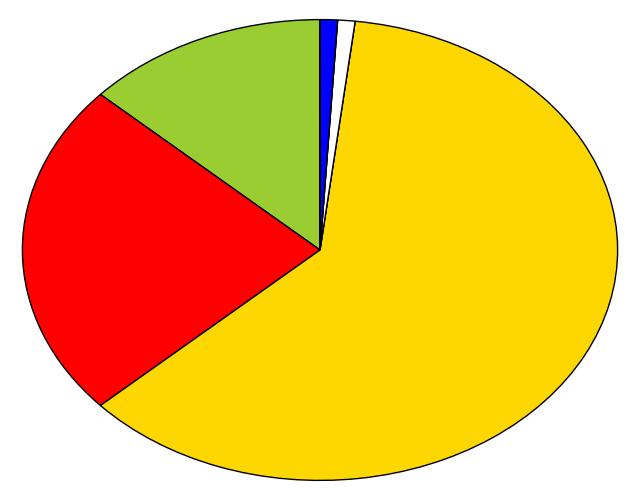
\includegraphics[width=\textwidth]{arousalALLpearsonR}
    \caption{Pearson correlation}
  \end{subfigure}
  \hfill
  \begin{subfigure}[b]{0.3\textwidth}
    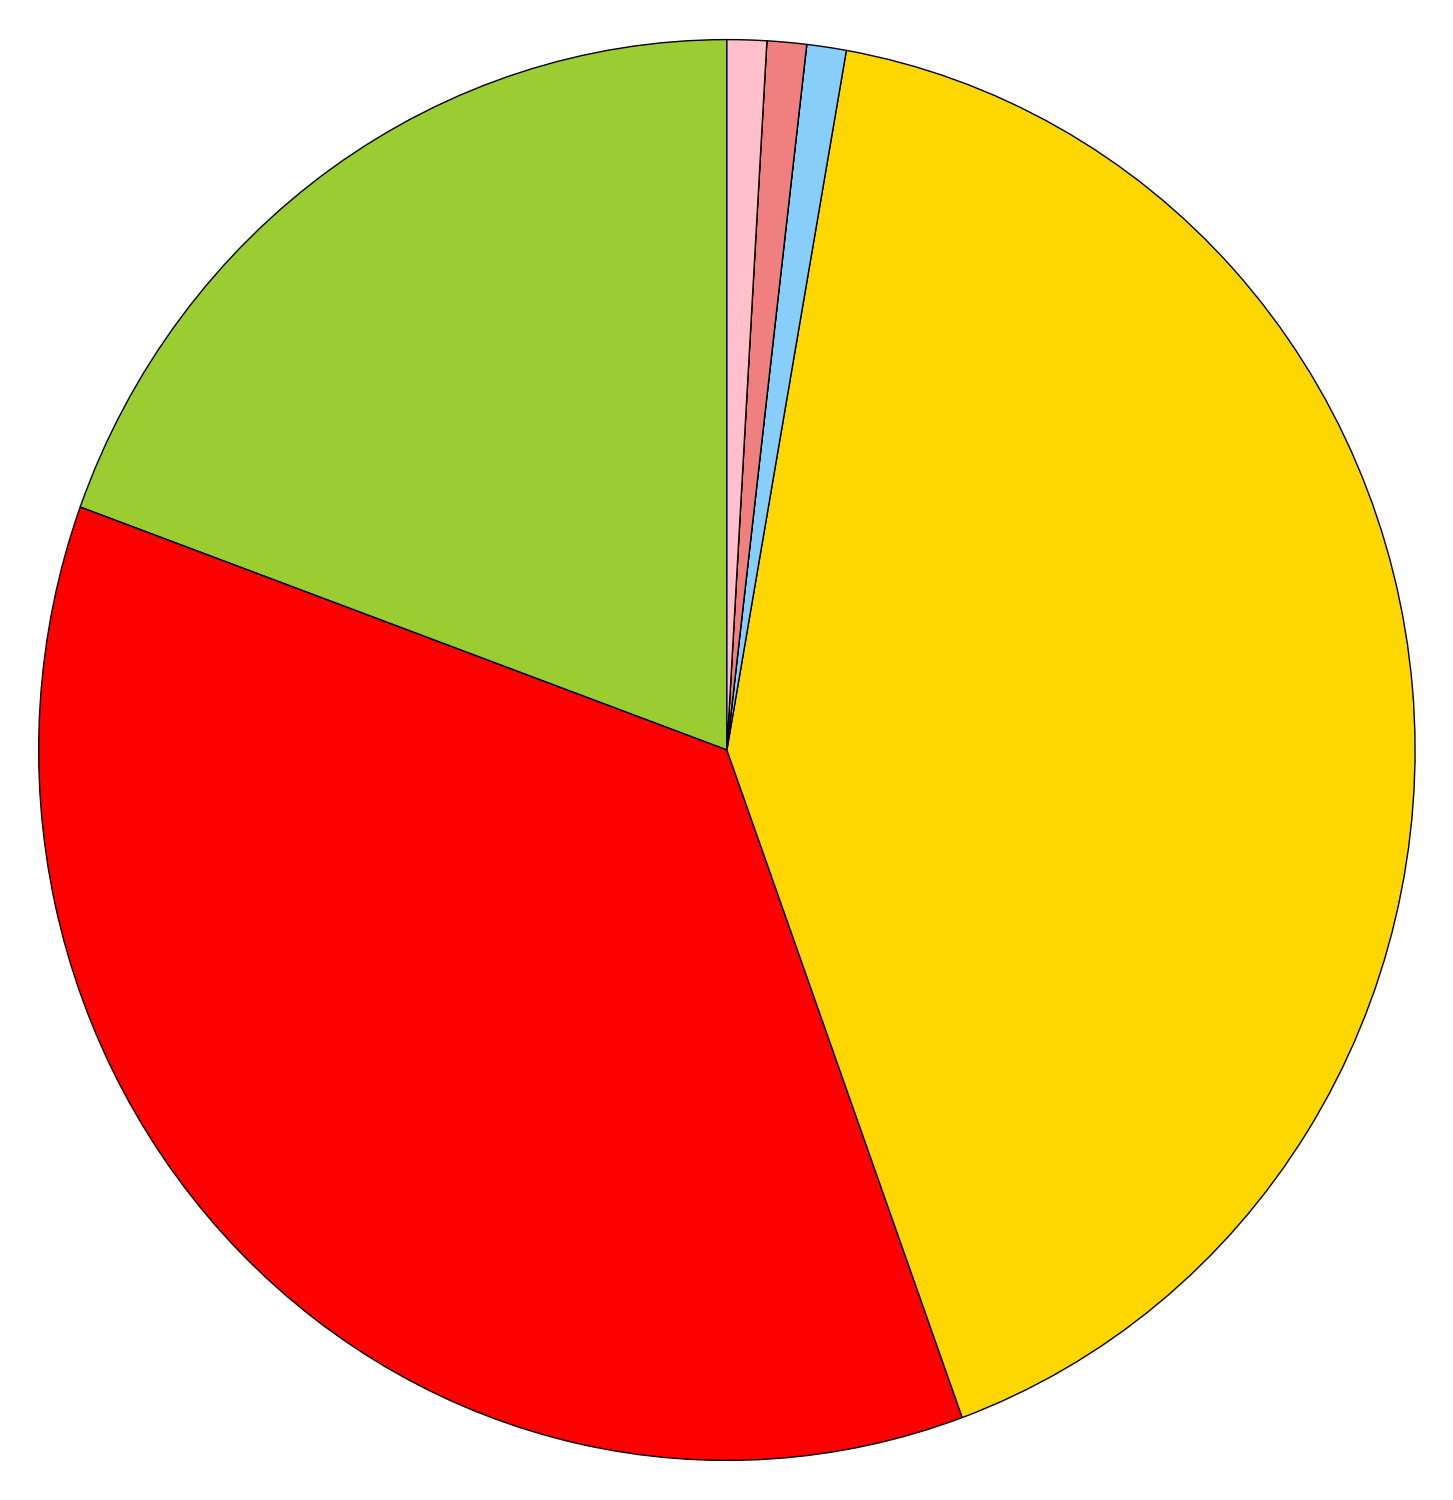
\includegraphics[width=\textwidth]{arousalALLMutInf}
    \caption{Mutual information}
  \end{subfigure}
  \hfill
  \begin{subfigure}[b]{0.3\textwidth}
    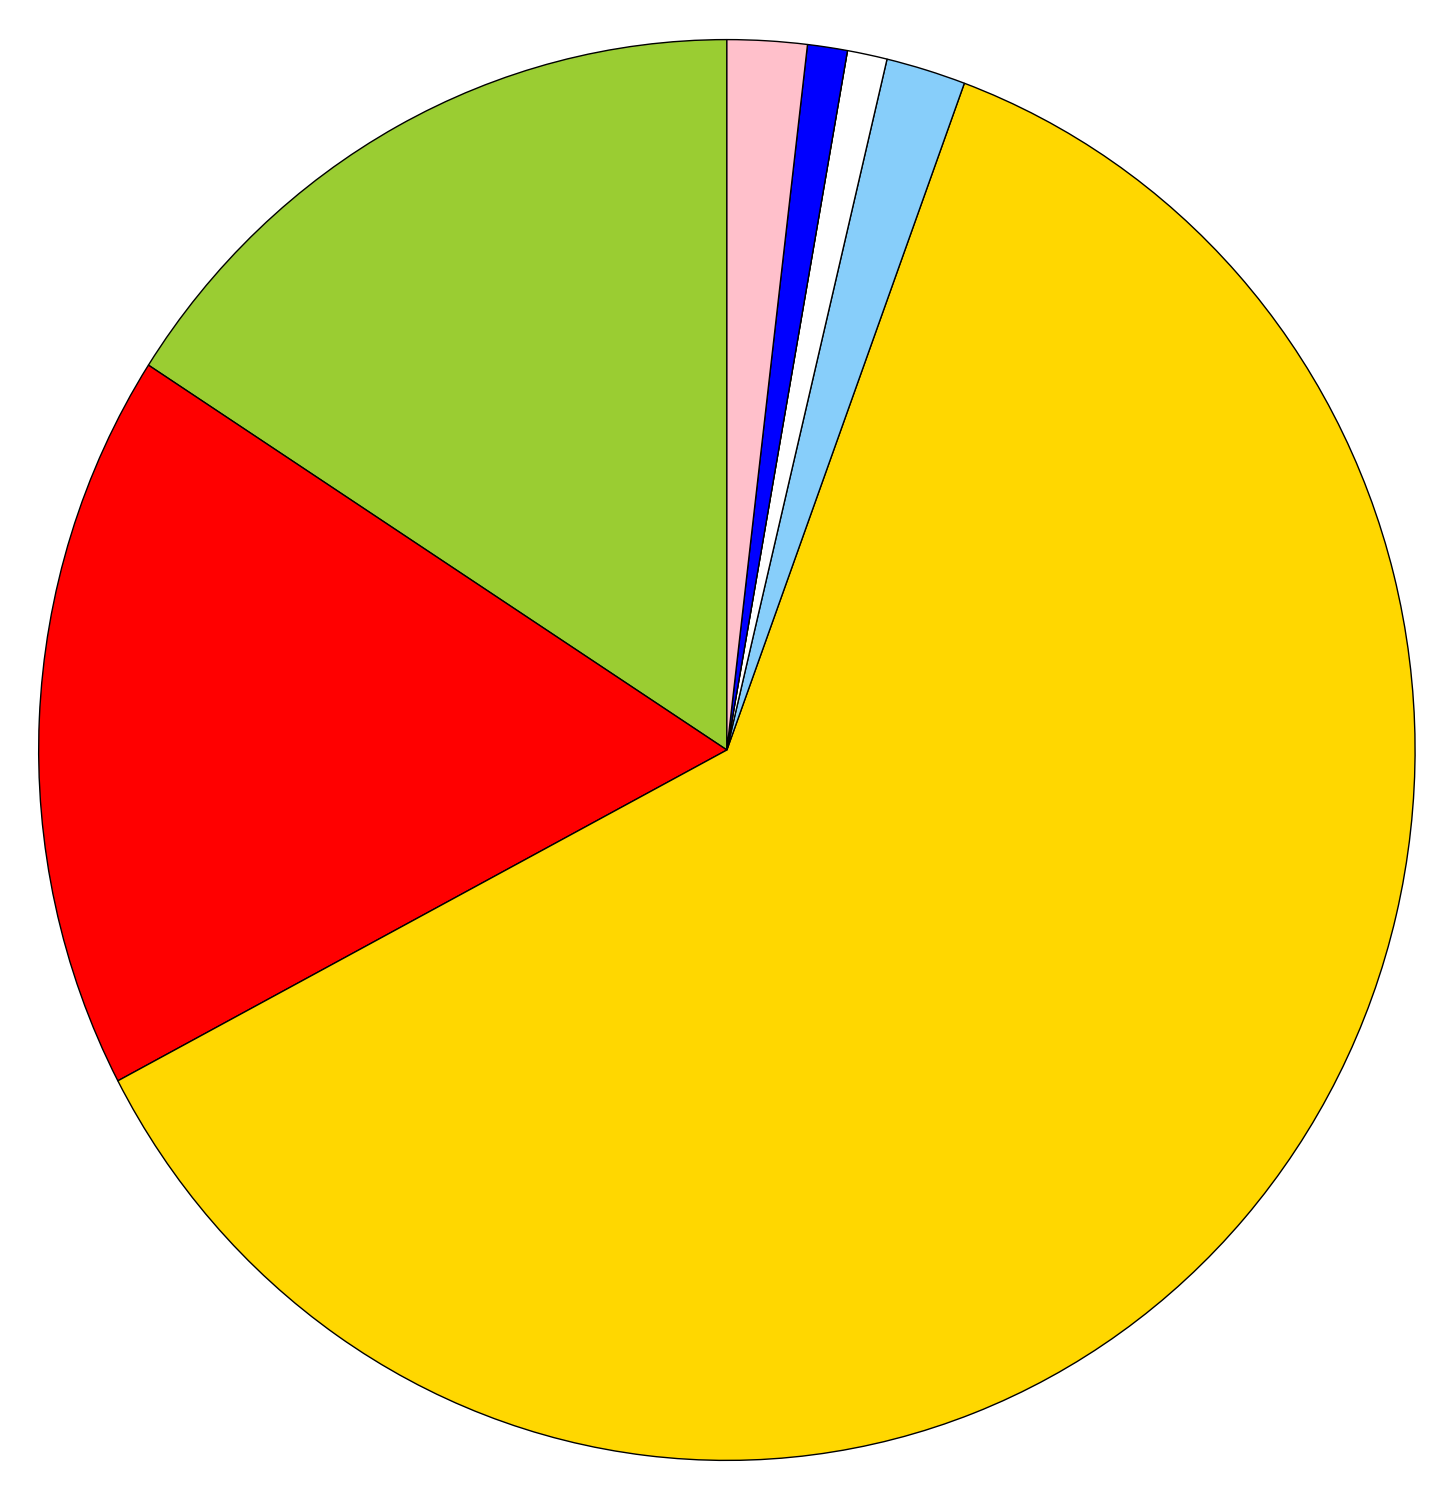
\includegraphics[width=\textwidth]{arousalALLdCorr}
    \caption{Distance Correlation}
  \end{subfigure}
  
  \begin{subfigure}[b]{0.3\textwidth}
    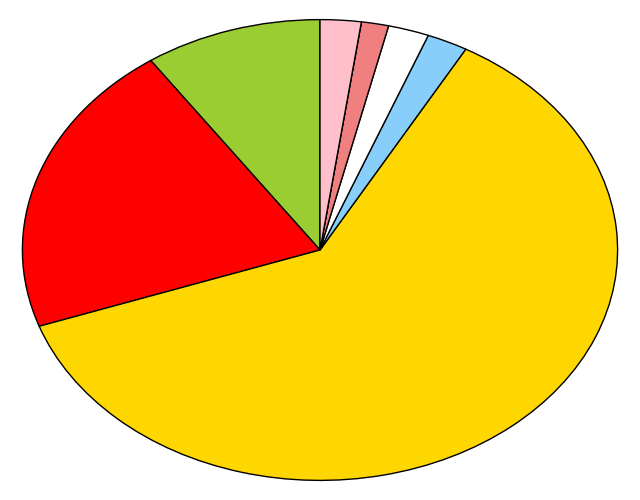
\includegraphics[width=\textwidth]{arousalALLANOVA}
    \caption{ANOVA}
  \end{subfigure}
  \hfill
  \begin{subfigure}[b]{0.3\textwidth}
    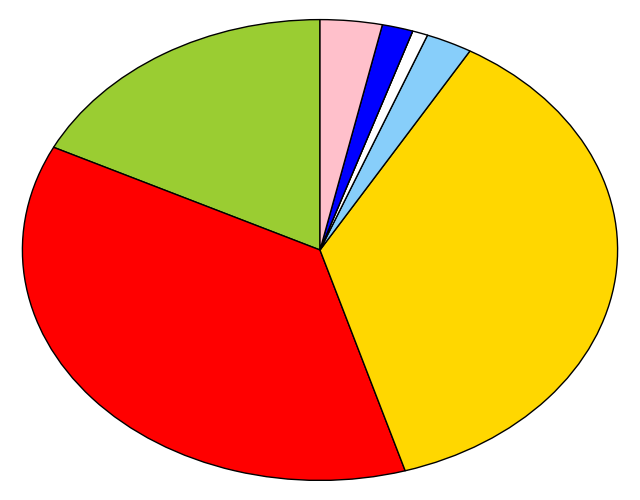
\includegraphics[width=\textwidth]{arousalALLLR}
    \caption{Linear regression}
  \end{subfigure}
  \hfill
  \begin{subfigure}[b]{0.3\textwidth}
    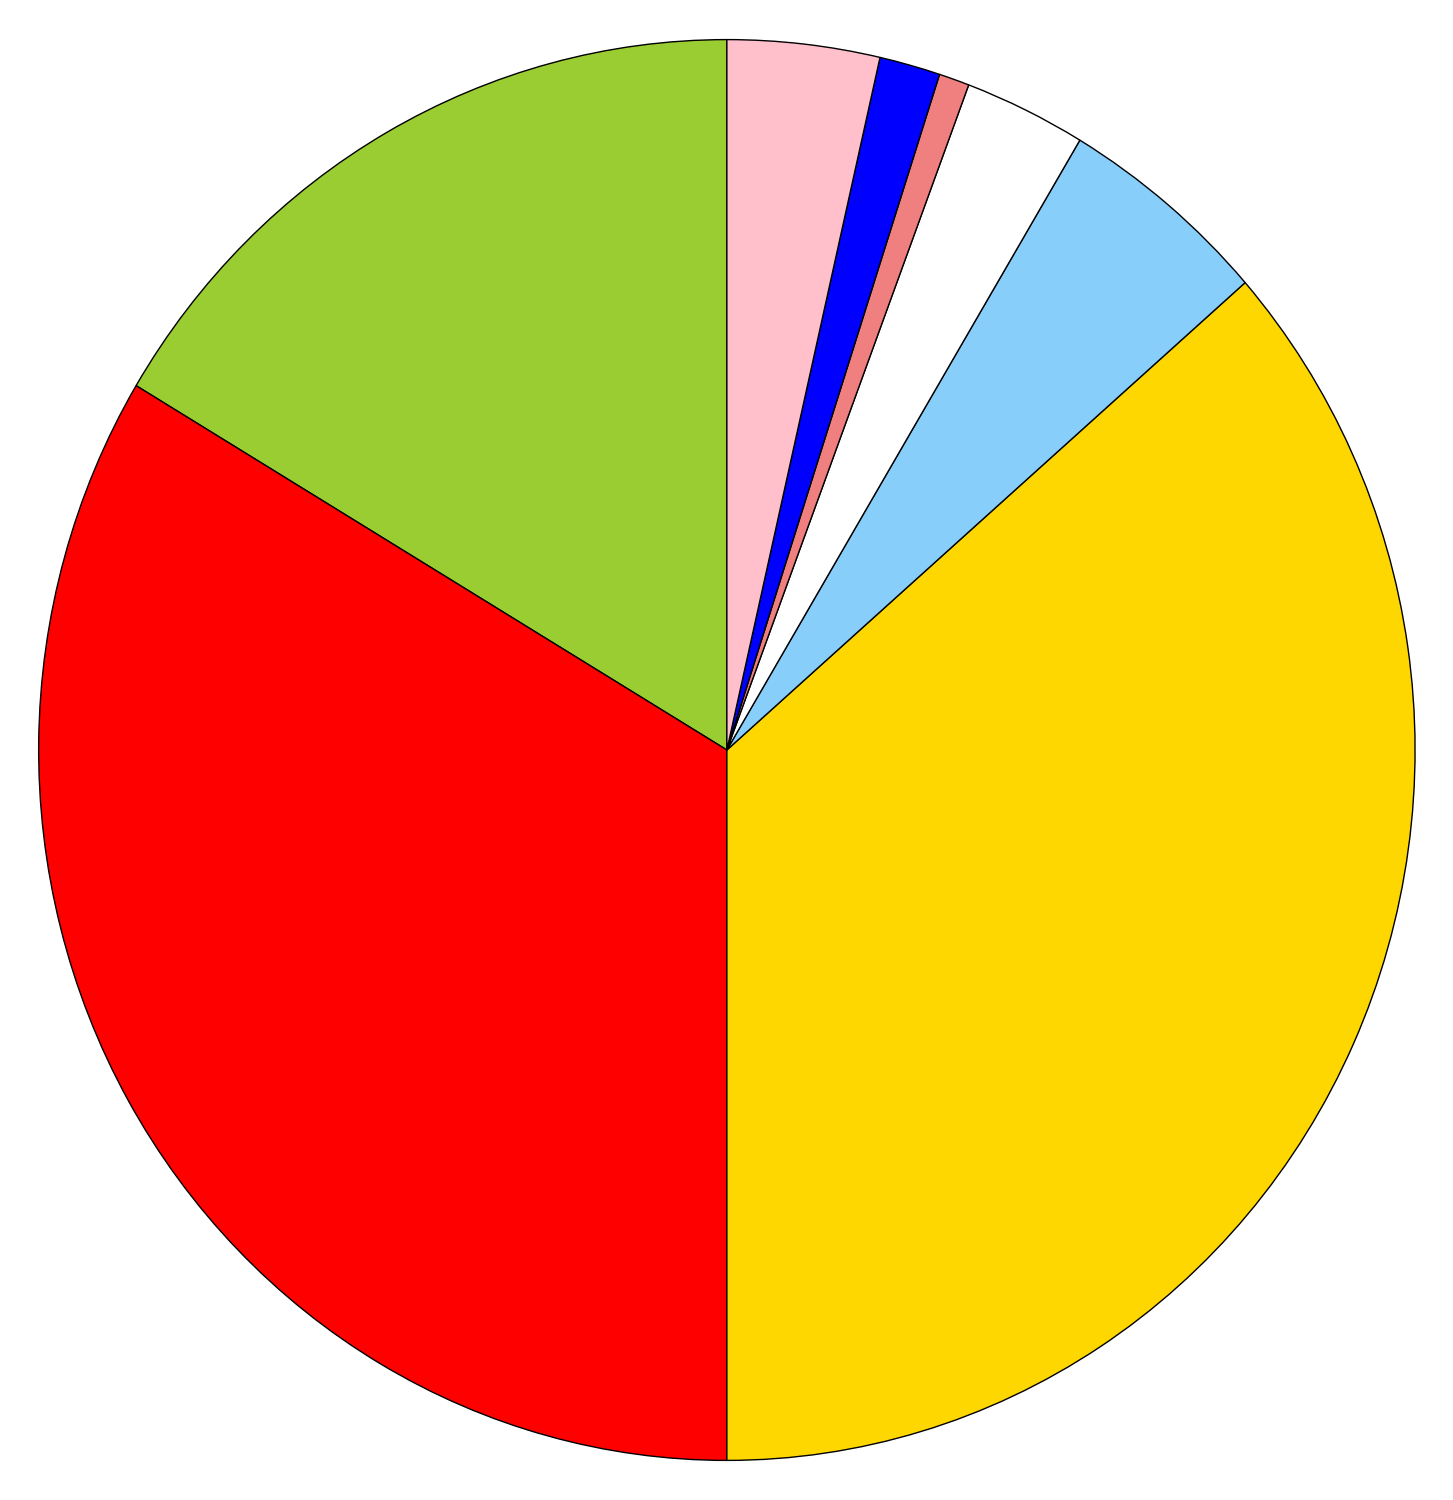
\includegraphics[width=\textwidth]{arousalALLSVM}
    \caption{SVM}
  \end{subfigure}
  
  \begin{subfigure}[b]{0.3\textwidth}
    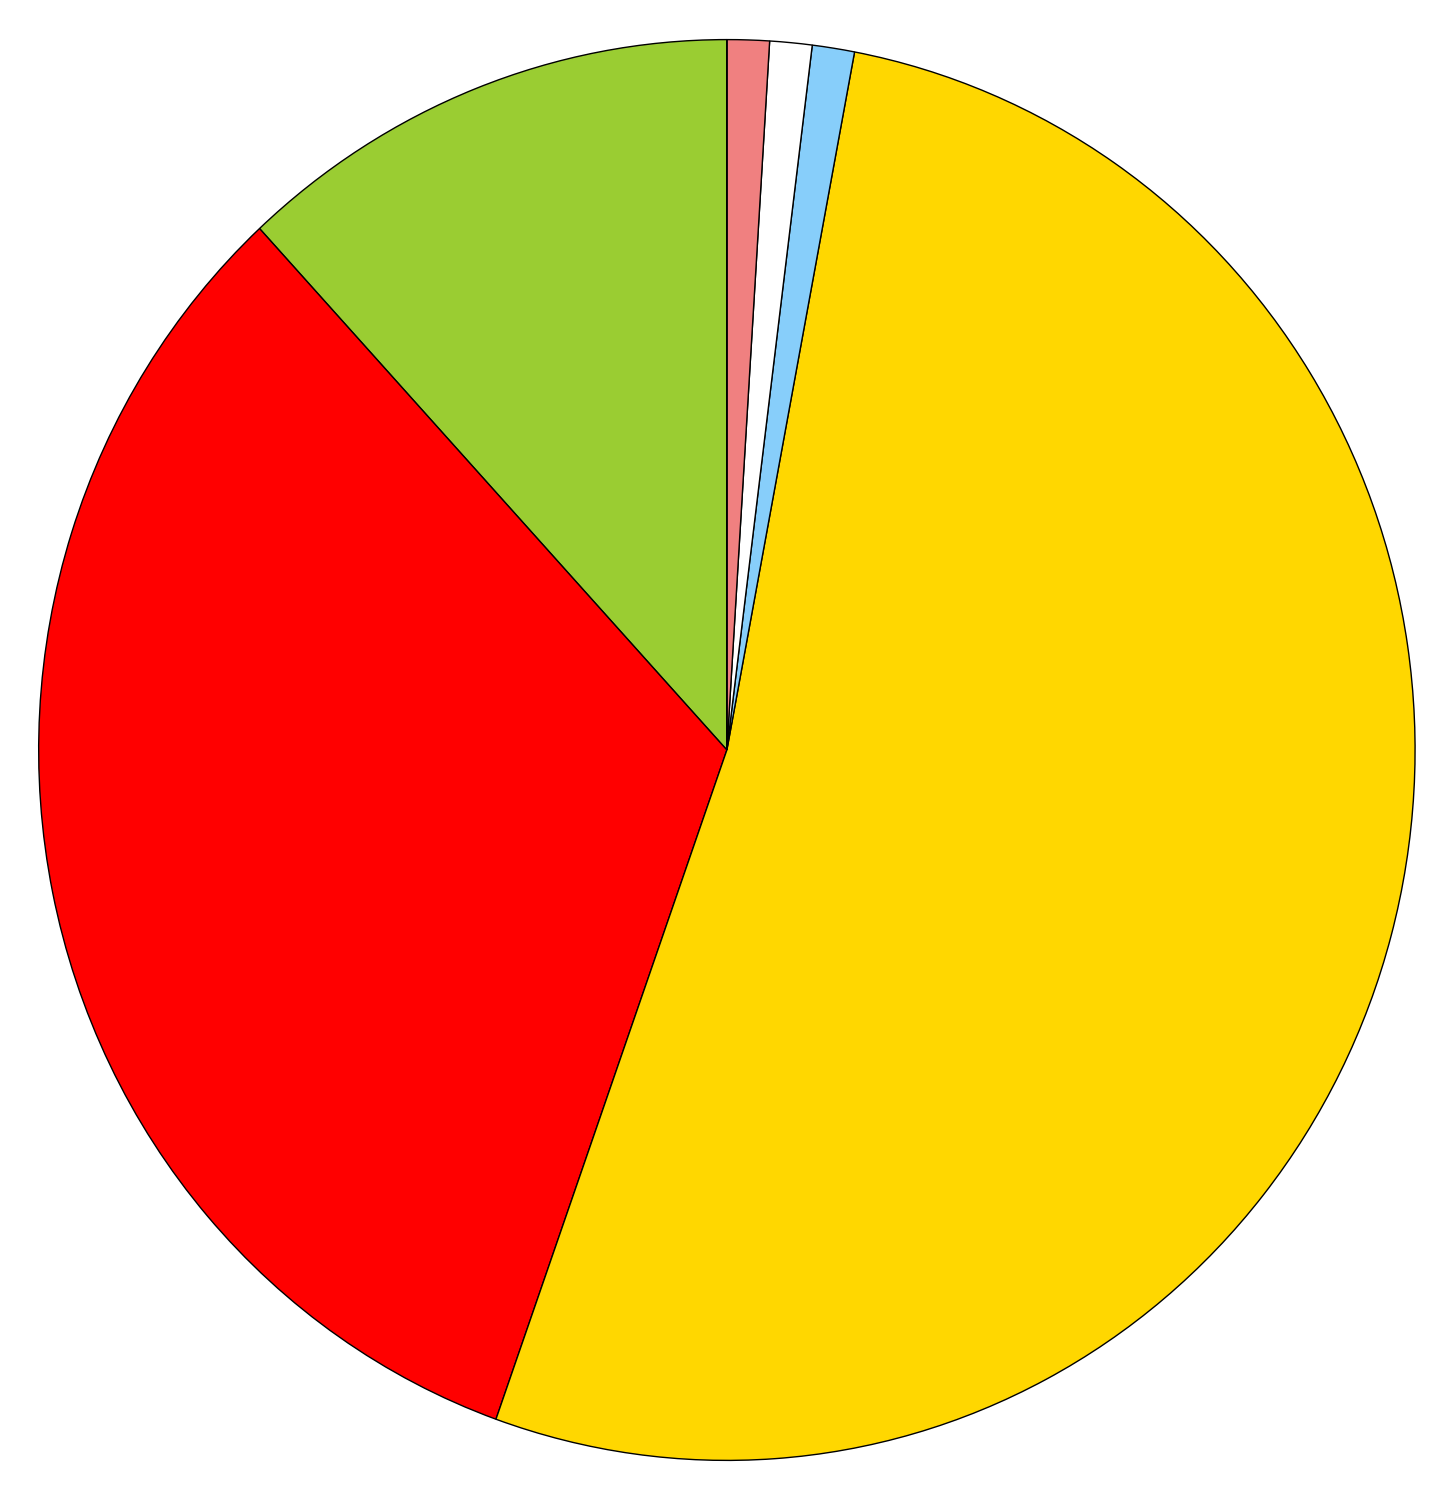
\includegraphics[width=\textwidth]{arousalALLLDA}
    \caption{LDA}
  \end{subfigure}
  \hfill
  \begin{subfigure}[b]{0.3\textwidth}
    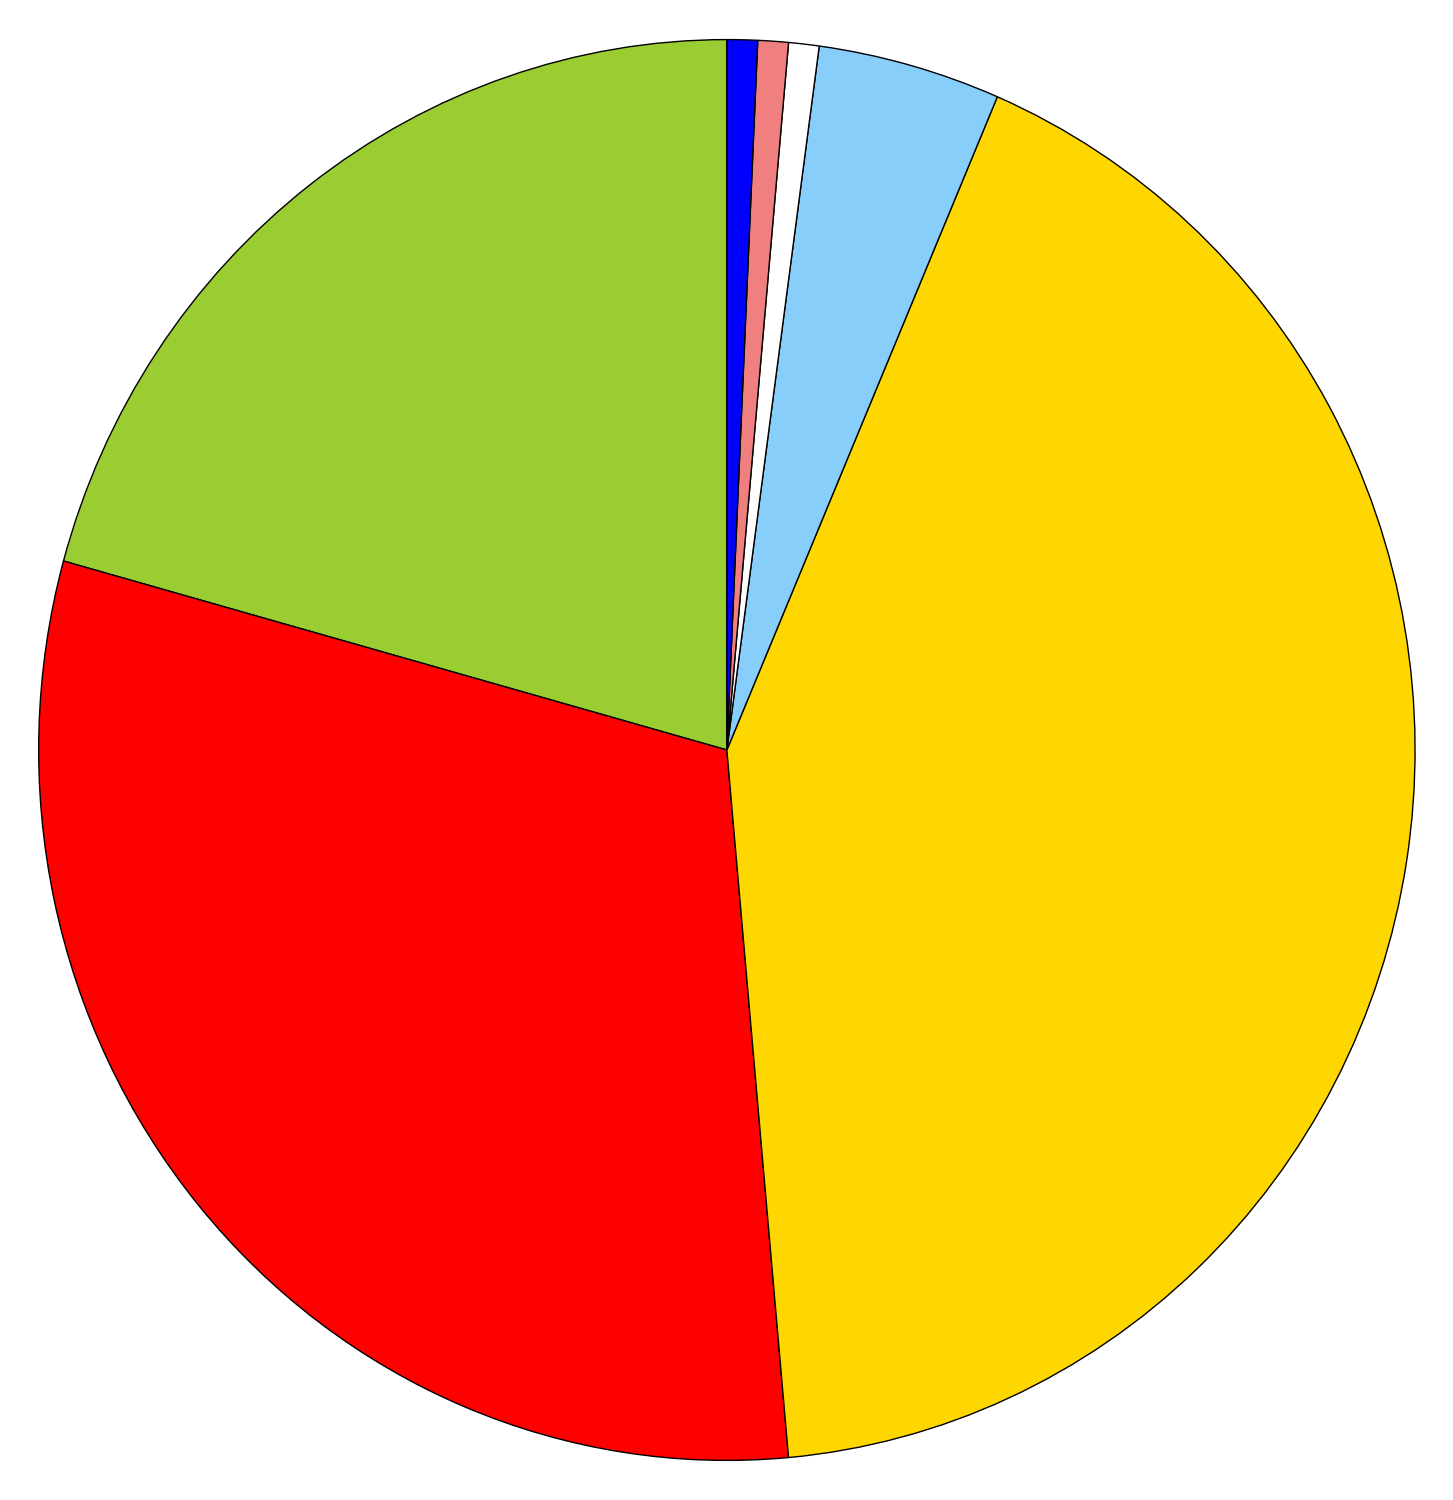
\includegraphics[width=\textwidth]{arousalALLL1}
    \caption{Lasso regression}
  \end{subfigure}
  \hfill
  \begin{subfigure}[b]{0.3\textwidth}
    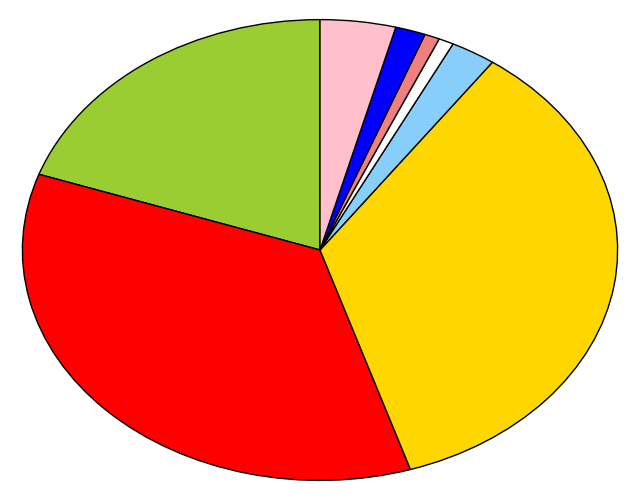
\includegraphics[width=\textwidth]{arousalALLL2}
    \caption{Ridge regression}
  \end{subfigure}
  
  \begin{subfigure}[b]{0.3\textwidth}
    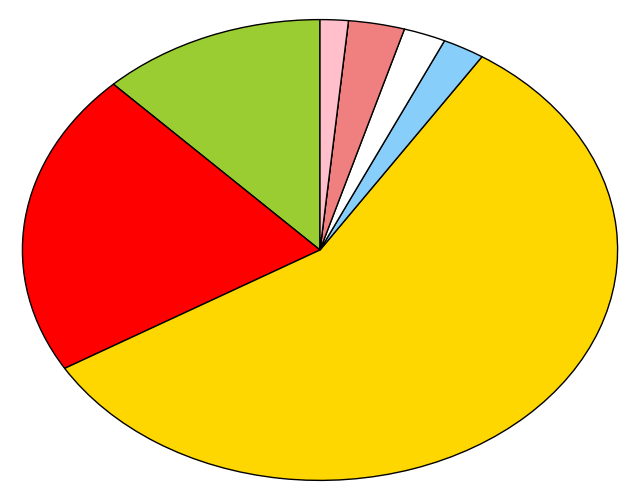
\includegraphics[width=\textwidth]{arousalALLRF}
    \caption{Random forests}
  \end{subfigure}
  \hfill
  \begin{subfigure}[b]{0.3\textwidth}
    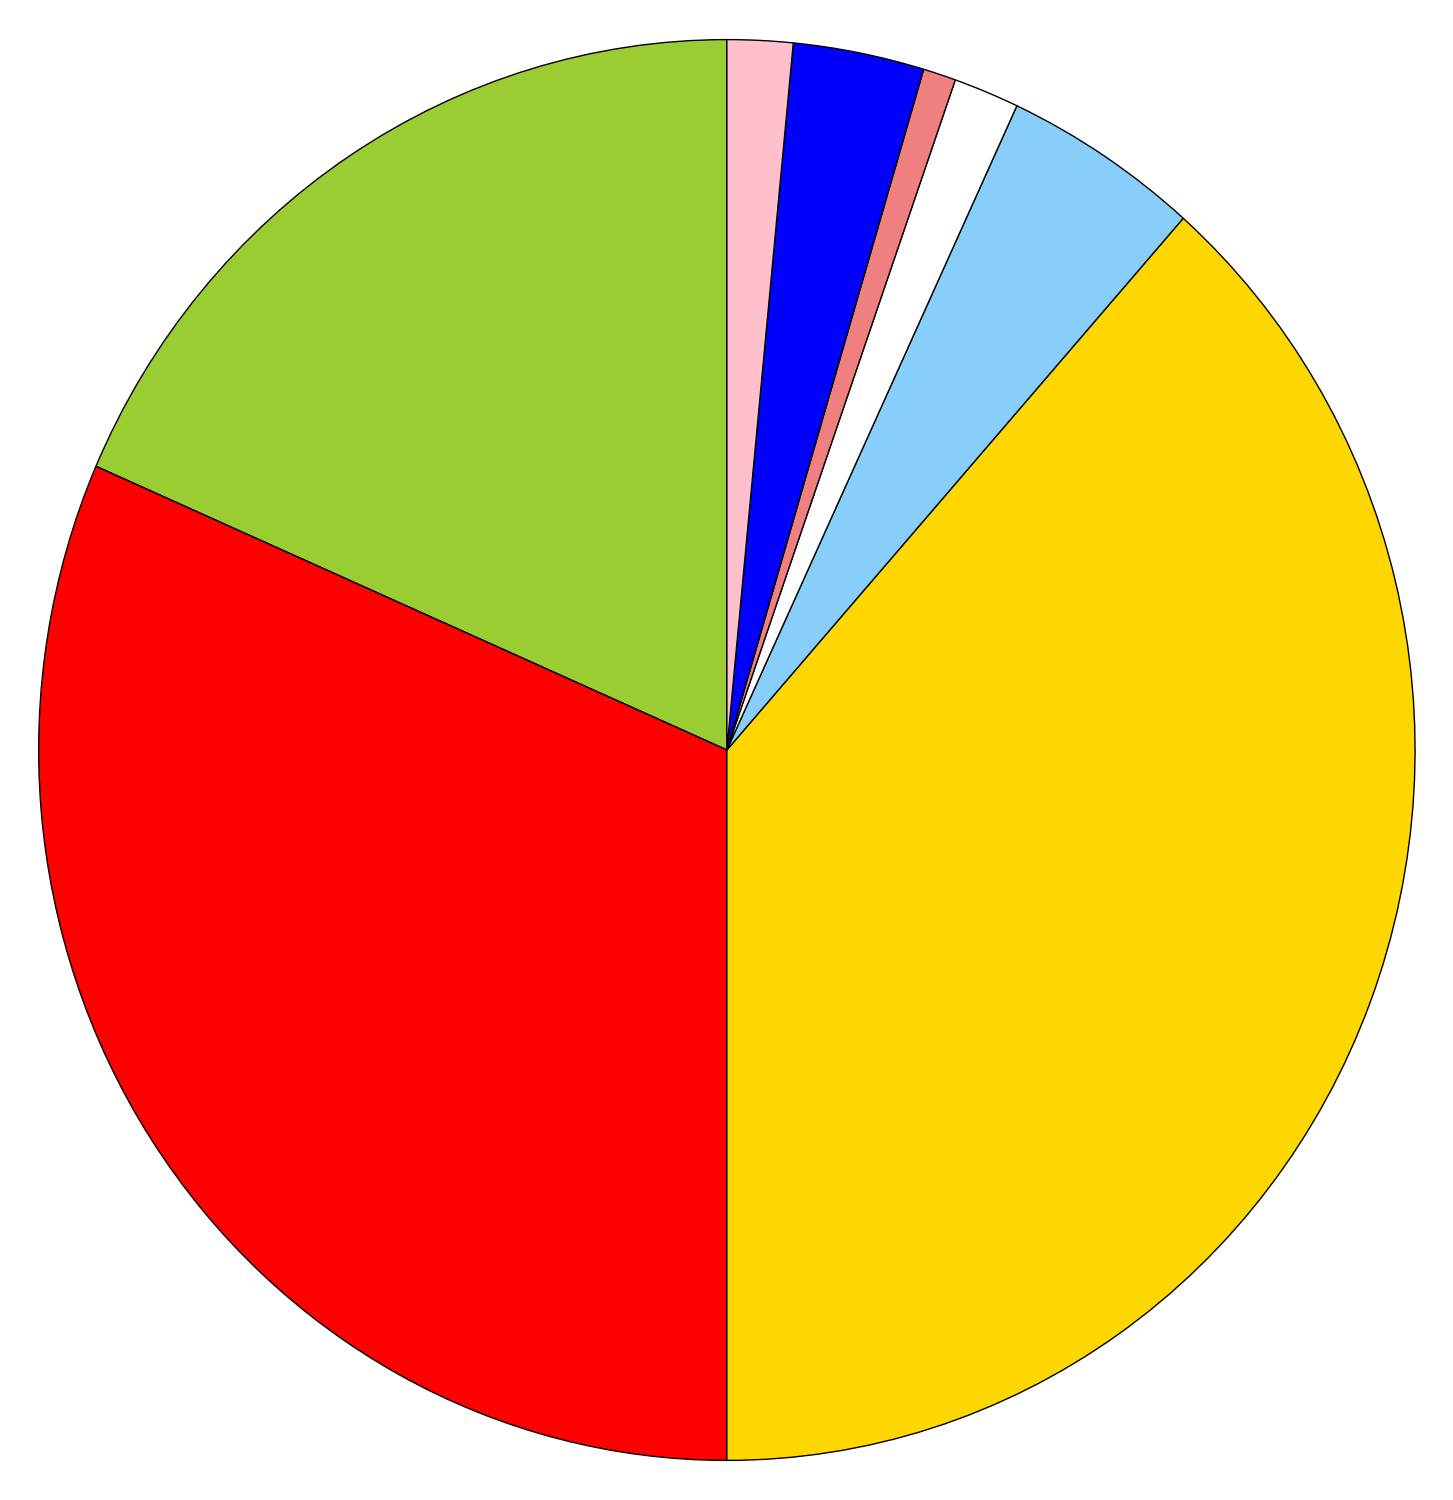
\includegraphics[width=\textwidth]{arousalALLPCA}
    \caption{PCA}
  \end{subfigure}
  \hfill
  \begin{subfigure}[b]{0.3\textwidth}
    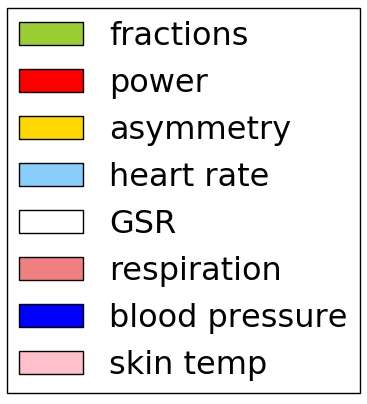
\includegraphics[width=\textwidth]{legend}
    \caption{Legend\label{arousalpieslegend}}
  \end{subfigure}
\caption{The distribution of the selected features for arousal classification of all persons combined of different feature selection methods. It is clear that the most valuable features are the asymmetry features combined with the power features. Furthermore, all feature selection methods agree that EEG features are dominant.\label{arousalpies}}
\end{figure}

\clearpage

\begin{figure}[!tbp]
  \centering
  \begin{subfigure}[b]{0.3\textwidth}
    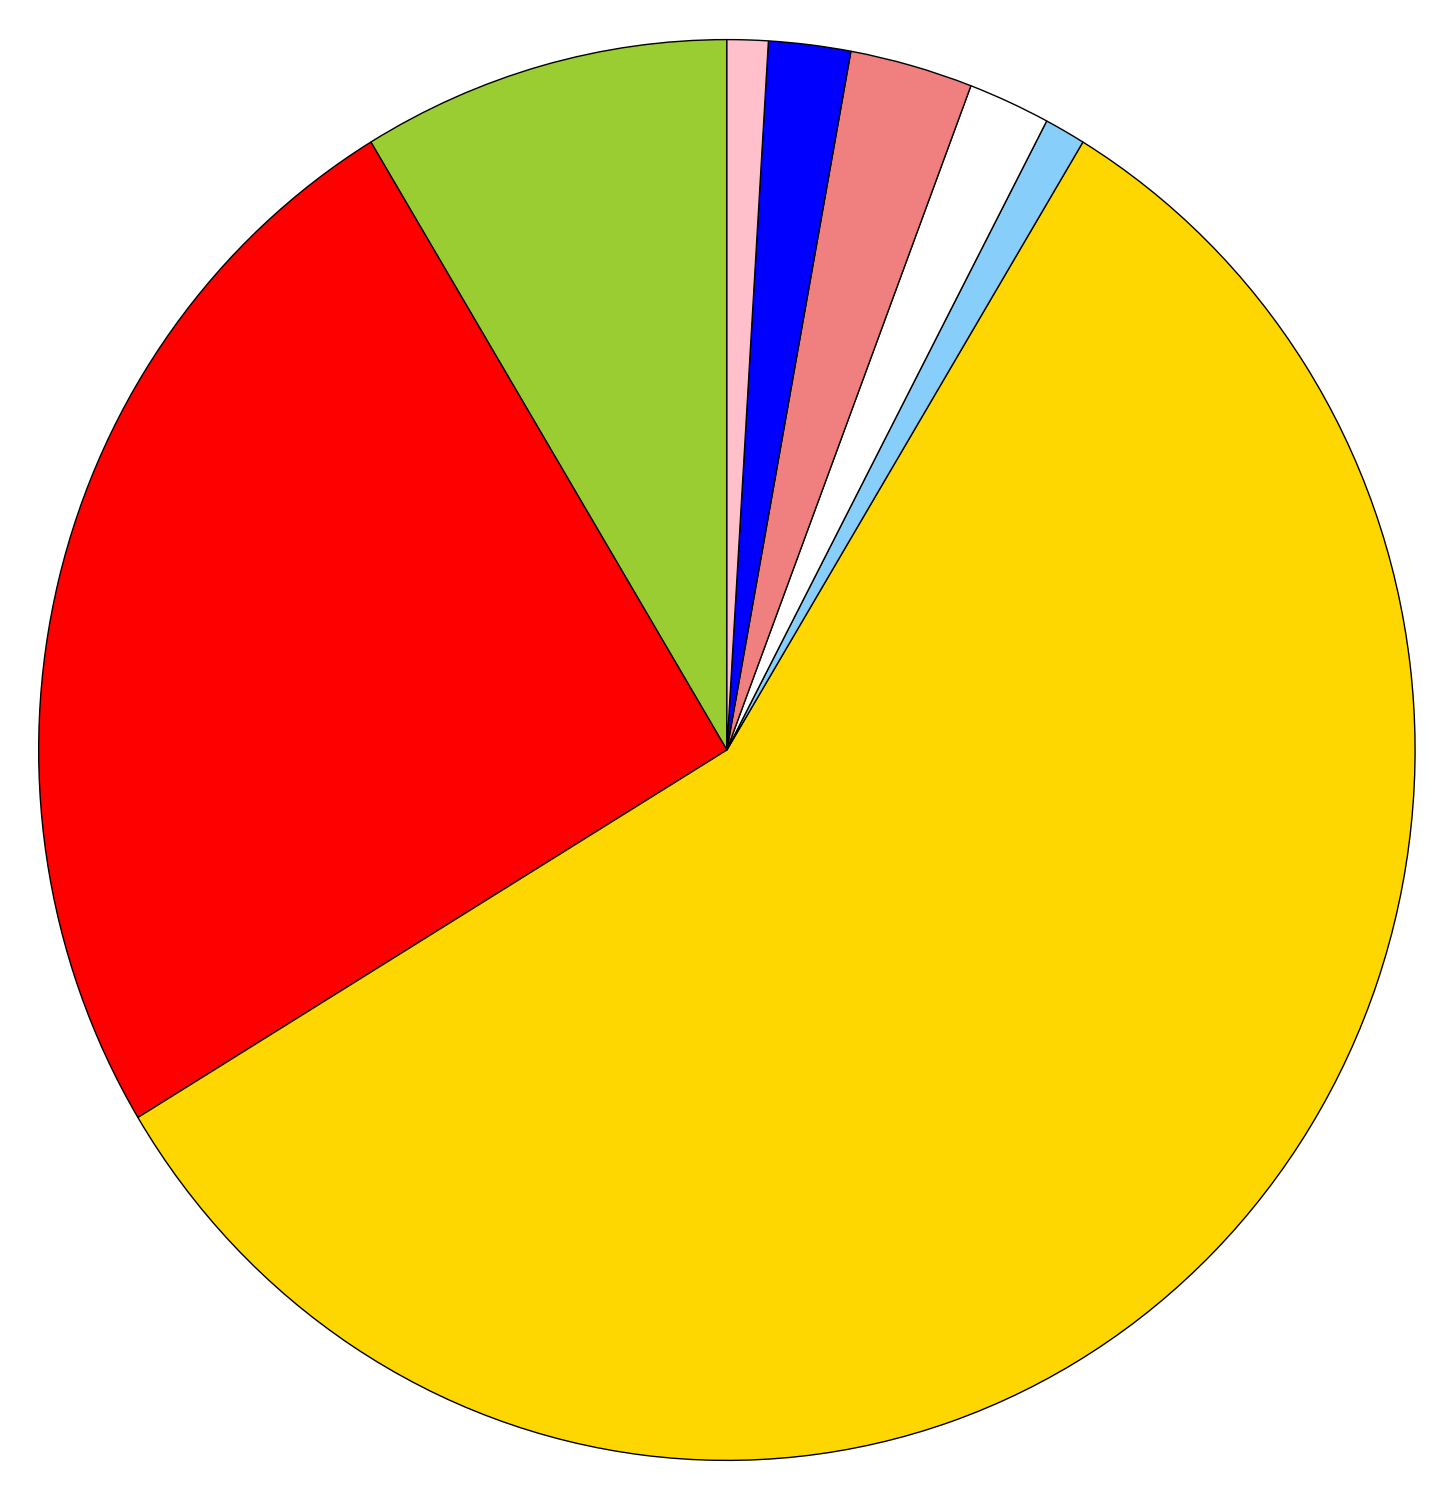
\includegraphics[width=\textwidth]{valenceALLpearsonR}
    \caption{Pearson correlation}
  \end{subfigure}
  \hfill
  \begin{subfigure}[b]{0.3\textwidth}
    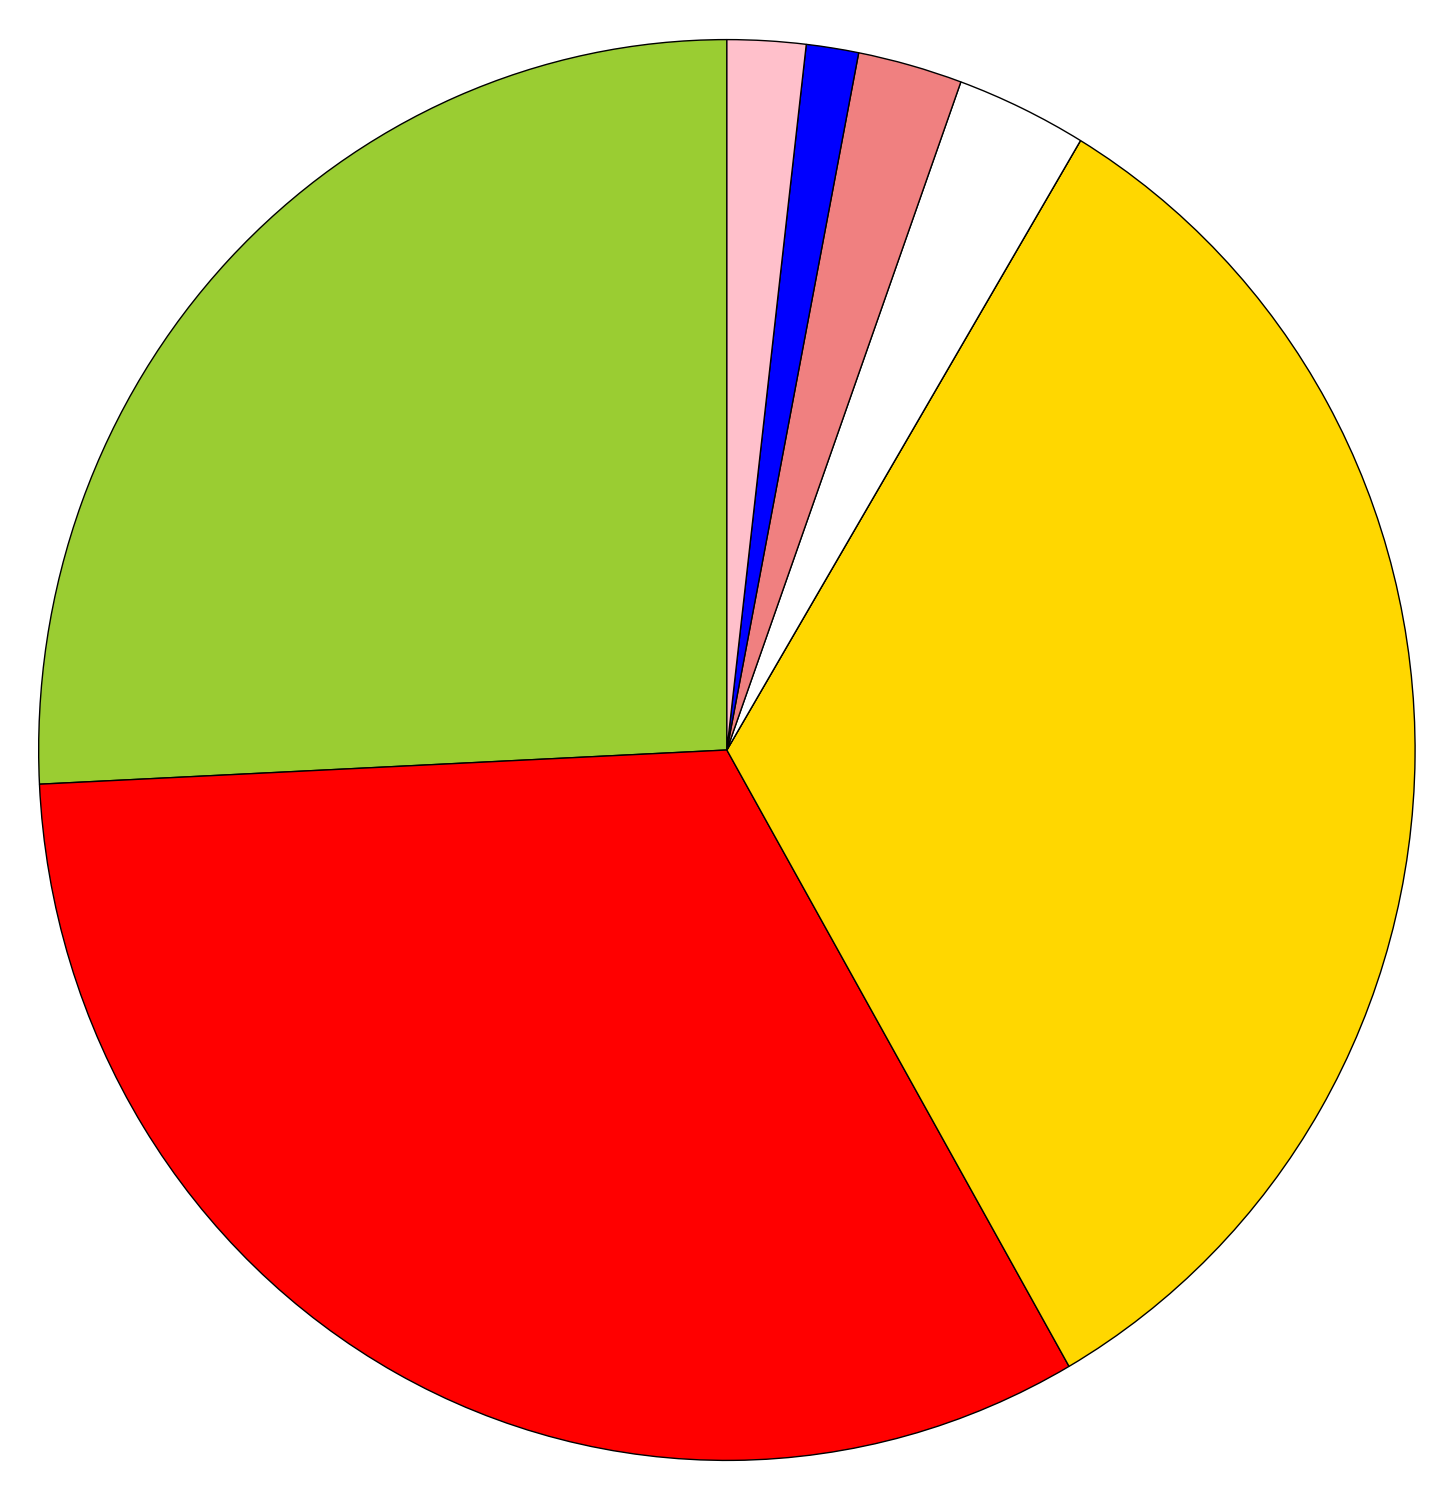
\includegraphics[width=\textwidth]{valenceALLMutInf}
    \caption{Mutual information}
  \end{subfigure}
  \hfill
  \begin{subfigure}[b]{0.3\textwidth}
    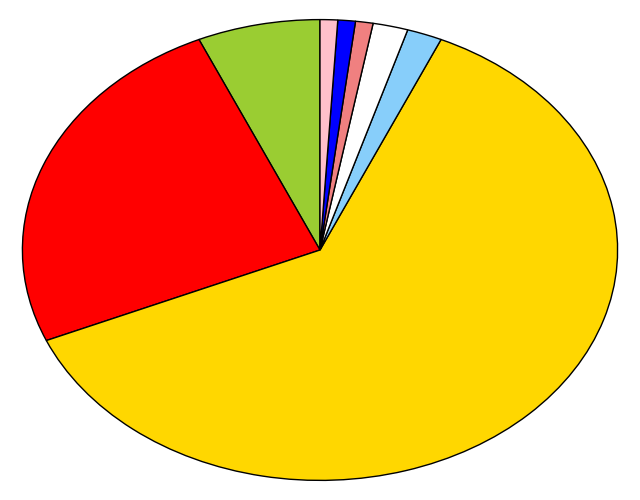
\includegraphics[width=\textwidth]{valenceALLdCorr}
    \caption{Distance Correlation}
  \end{subfigure}
  
  \begin{subfigure}[b]{0.3\textwidth}
    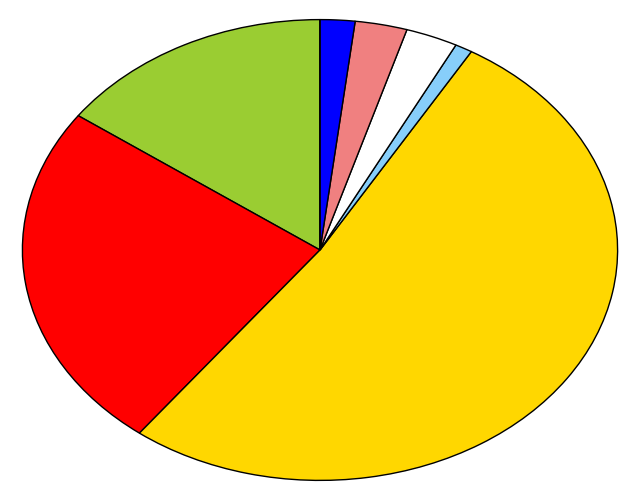
\includegraphics[width=\textwidth]{valenceALLANOVA}
    \caption{ANOVA}
  \end{subfigure}
  \hfill
  \begin{subfigure}[b]{0.3\textwidth}
    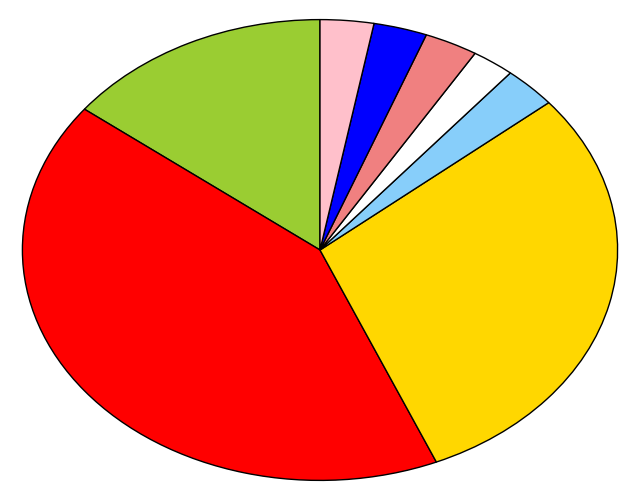
\includegraphics[width=\textwidth]{valenceALLLR}
    \caption{Linear regression}
  \end{subfigure}
  \hfill
  \begin{subfigure}[b]{0.3\textwidth}
    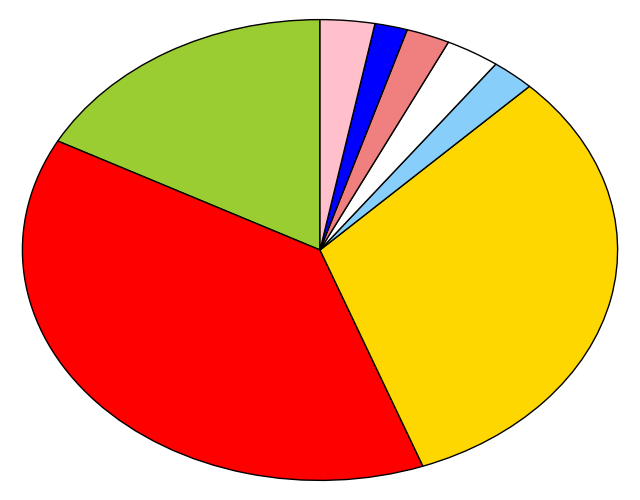
\includegraphics[width=\textwidth]{valenceALLSVM}
    \caption{SVM}
  \end{subfigure}
  
  \begin{subfigure}[b]{0.3\textwidth}
    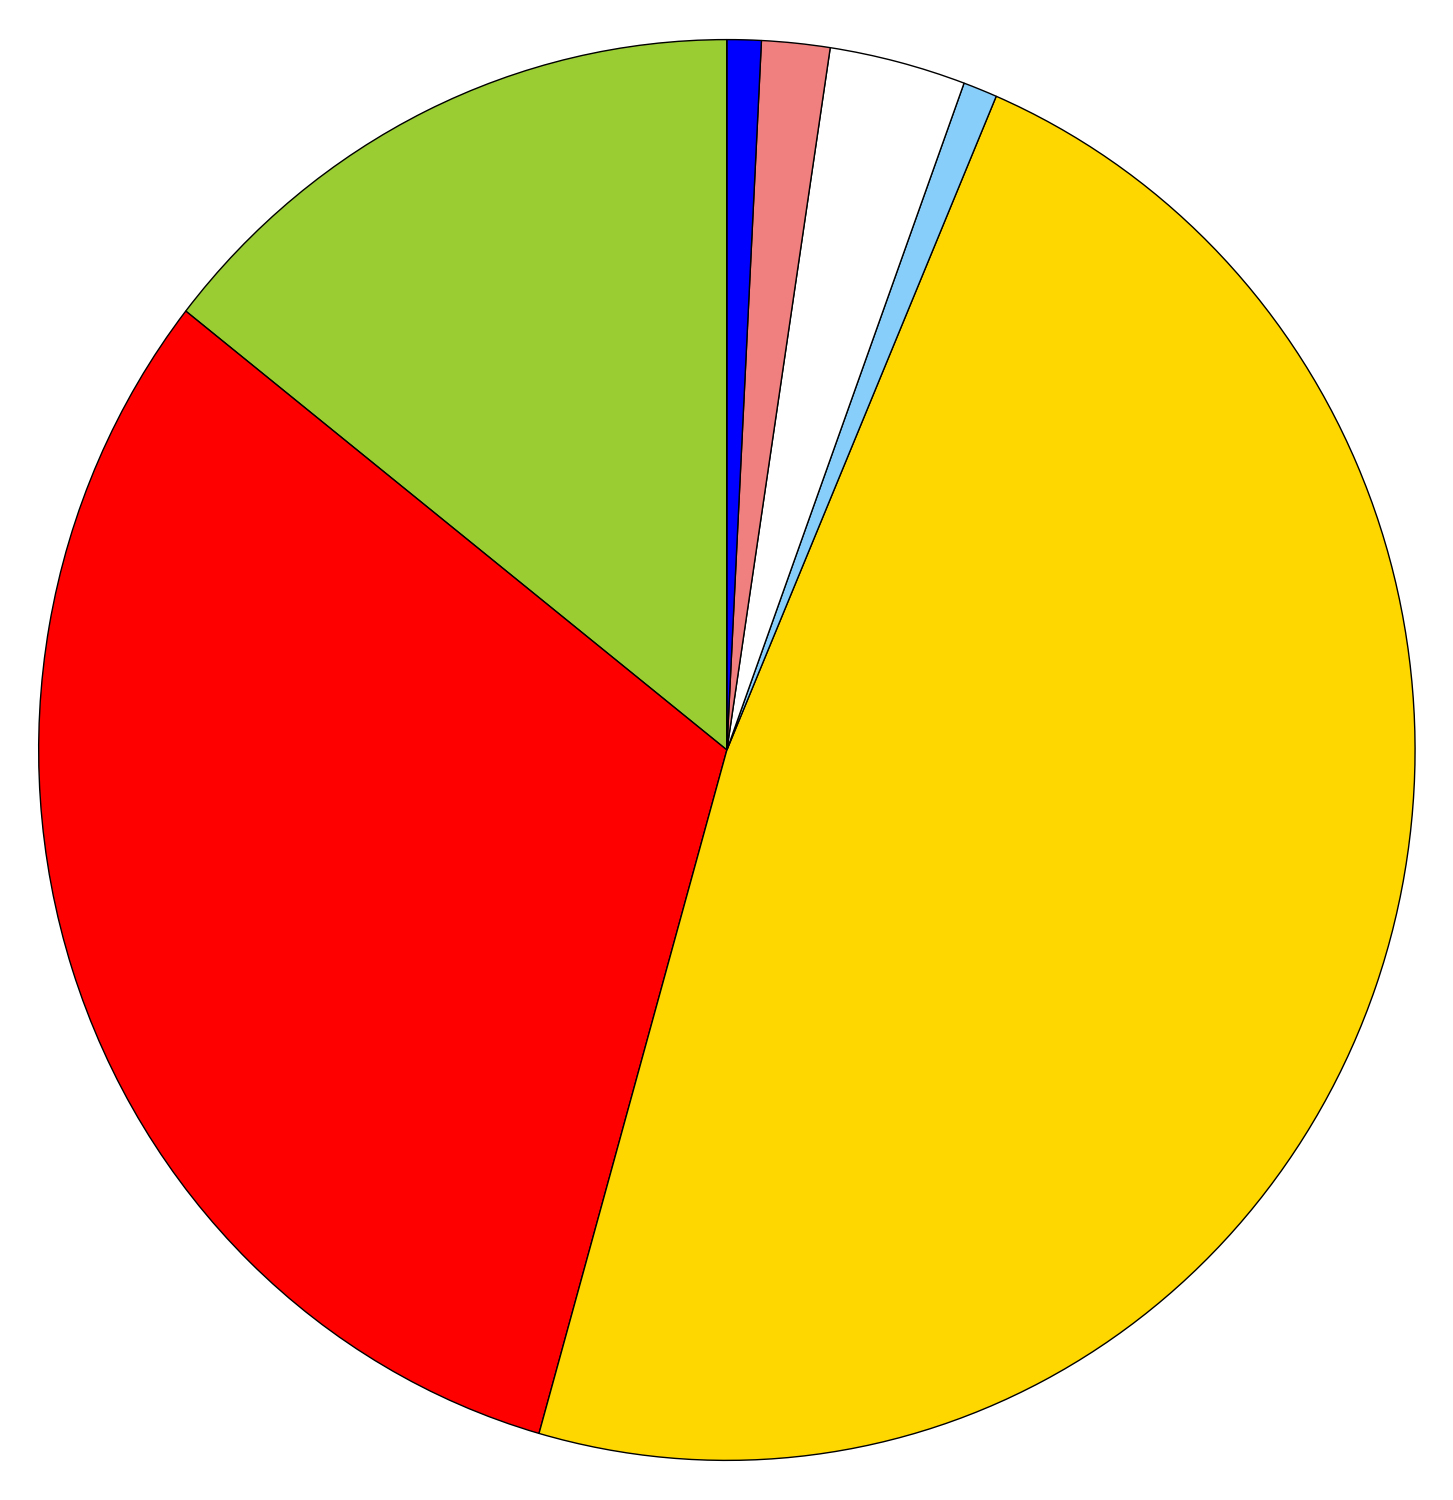
\includegraphics[width=\textwidth]{valenceALLLDA}
    \caption{LDA}
  \end{subfigure}
  \hfill
  \begin{subfigure}[b]{0.3\textwidth}
    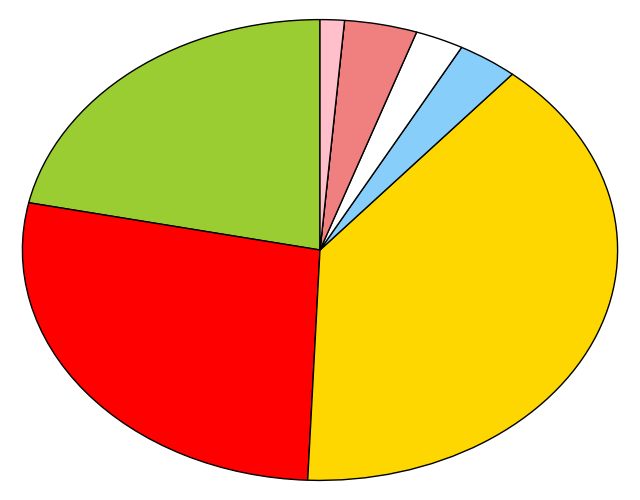
\includegraphics[width=\textwidth]{valenceALLL1}
    \caption{Lasso regression}
  \end{subfigure}
  \hfill
  \begin{subfigure}[b]{0.3\textwidth}
    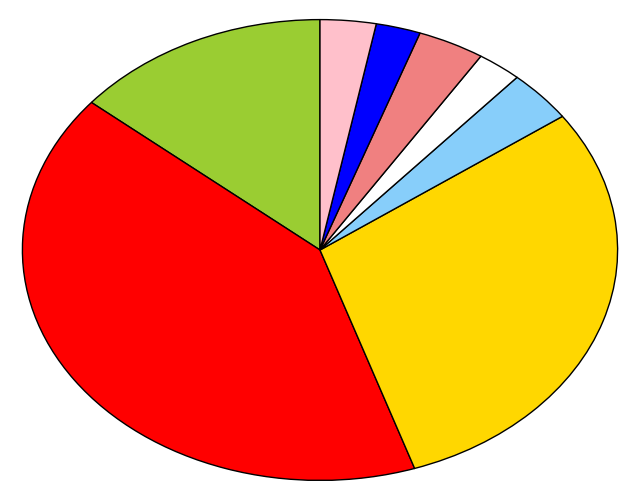
\includegraphics[width=\textwidth]{valenceALLL2}
    \caption{Ridge regression}
  \end{subfigure}
  
  \begin{subfigure}[b]{0.3\textwidth}
    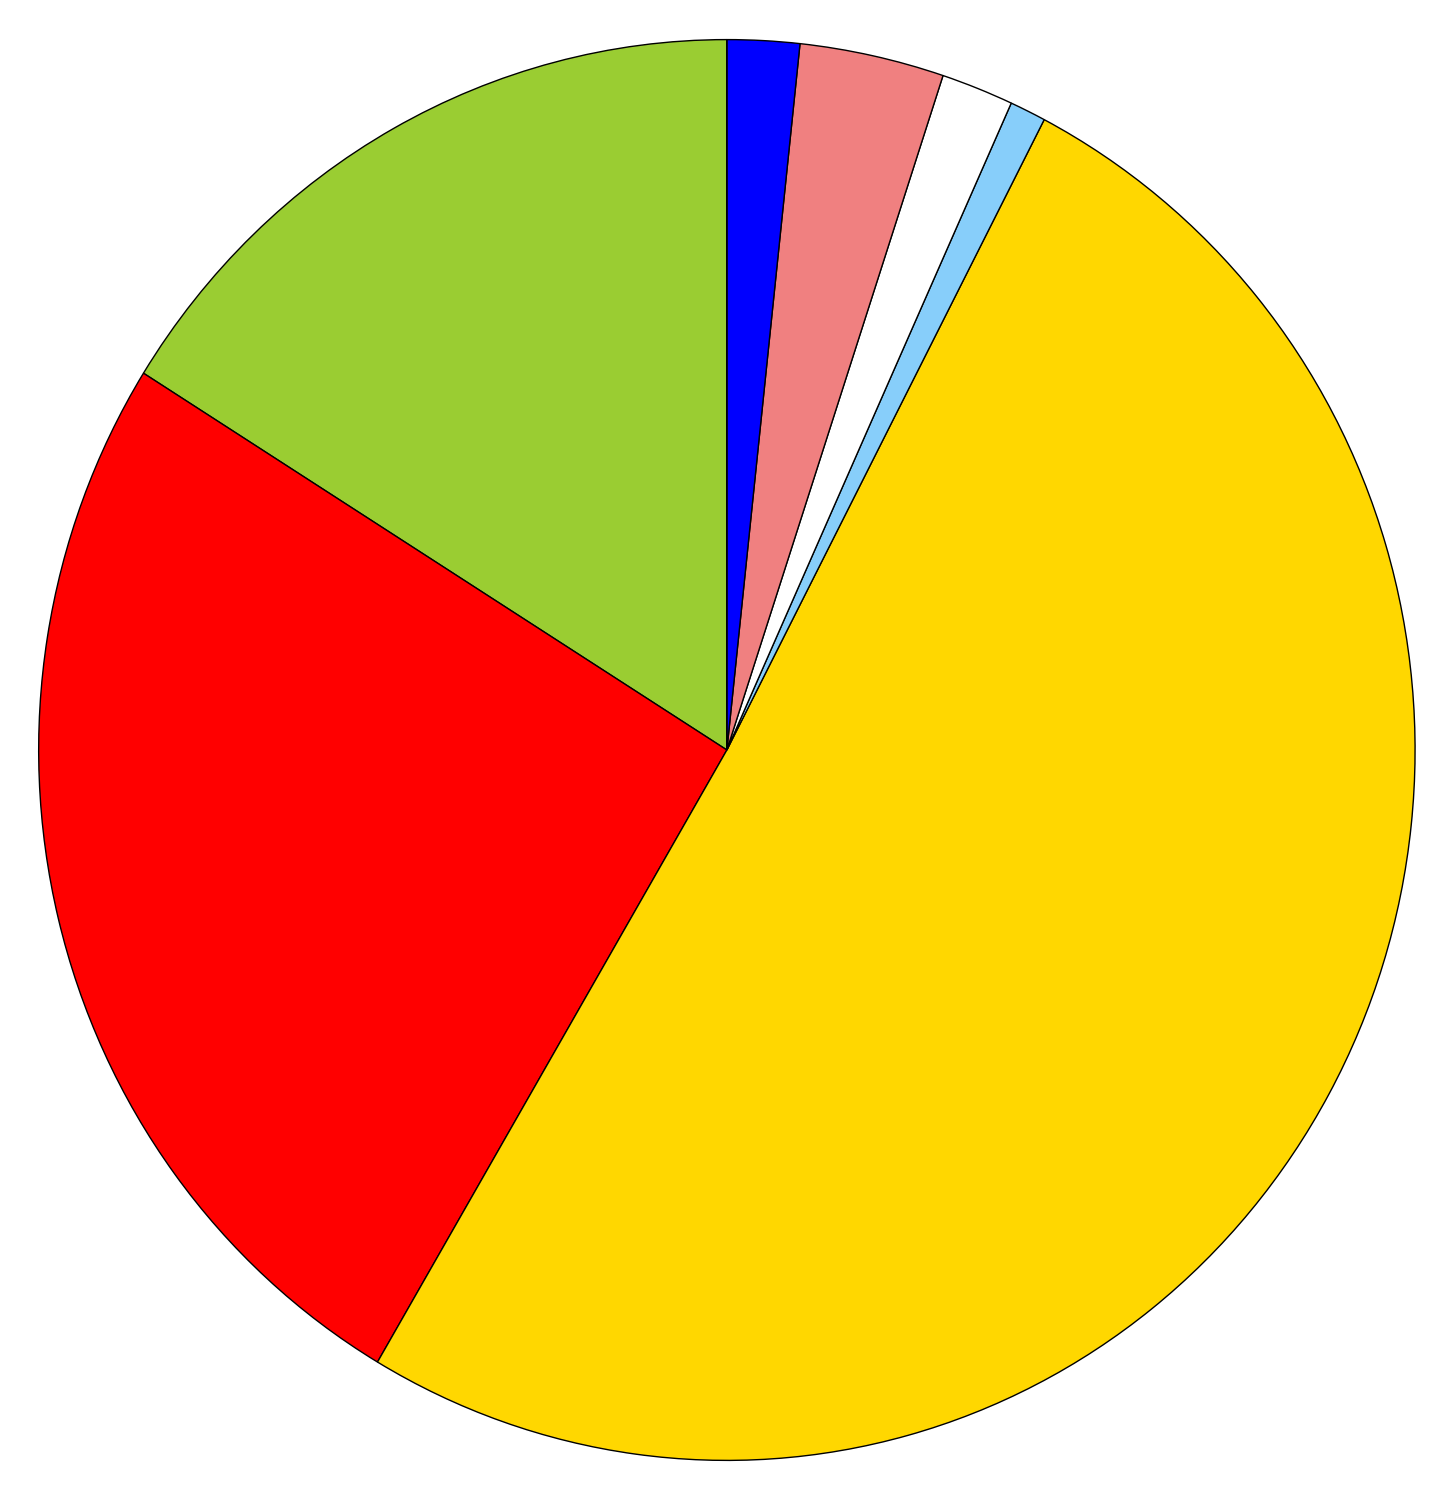
\includegraphics[width=\textwidth]{valenceALLRF}
    \caption{Random forests}
  \end{subfigure}
  \hfill
  \begin{subfigure}[b]{0.3\textwidth}
    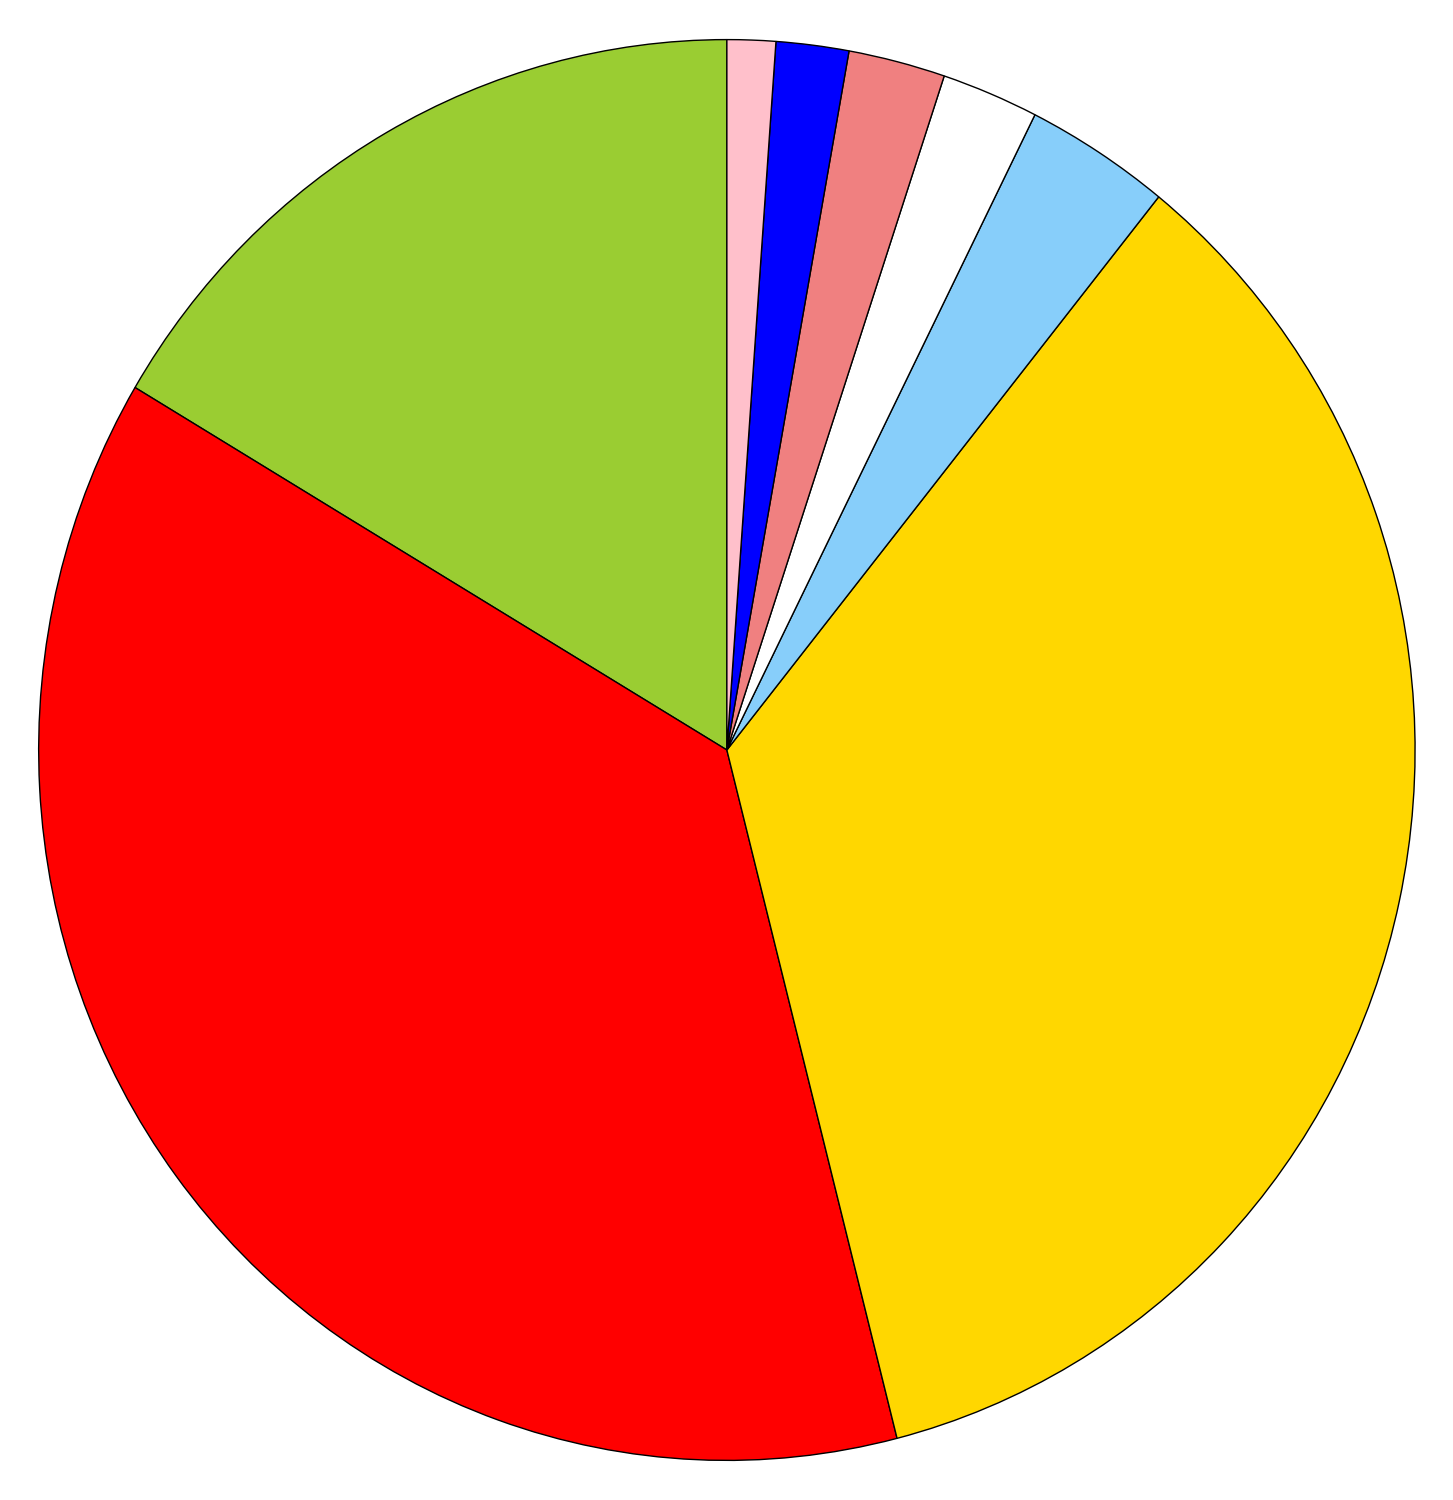
\includegraphics[width=\textwidth]{valenceALLPCA}
    \caption{PCA}
  \end{subfigure}
  \hfill
  \begin{subfigure}[b]{0.3\textwidth}
    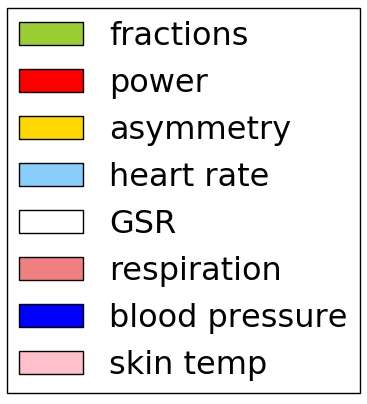
\includegraphics[width=\textwidth]{legend}
    \caption{Legend\label{valencepieslegend}}
  \end{subfigure}
\caption{The distribution of the selected features for valence classification of all persons combined of different feature selection methods. It is clear that the most valuable features are the asymmetry features combined with the power features. Furthermore, all feature selection methods agree that EEG features are dominant.\label{valencepies}}
\end{figure}
\clearpage

The fact that the non-EEG features are almost never chosen might indicate that they are less important. In an attempt to further investigate the difference between EEG features and non-EEG features, the performance of three different feature sets was compared. The first feature set is the previously used feature set with all possible features. The second and third feature sets contained only EEG and non-EEG features respectively. The feature selection was done with random forest, as this method had the best average performance and is the most advanced. 

\npar

The resulting performances of these different features sets are displayed in Figure \ref{arousalphyeegall} for arousal and in Figure \ref{valencephyeegall} for valence. The exact values are shown in Table \ref{phyeegalltable}.

\mijnfiguur{width=1.\textwidth}{arousalphyeegall}{The average and standard deviation of the test accuracies of arousal classification for all, EEG and non-EEG features, see also Table \ref{phyeegalltable}}

\mijnfiguur{width=1.\textwidth}{valencephyeegall}{The average and standard deviation of the test accuracies of valence classification for all, EEG and non-EEG features, see also Table \ref{phyeegalltable}}

\begin{table}[H]
\centering
\caption{The average and standard deviation of the test accuracies (over the different persons) for the different feature sets, using the random forest feature selection model.\label{phyeegalltable}}
\begin{tabular}{l|ll|ll}
         & \textbf{Arousal} &         & \textbf{Valence} &         \\
\textbf{Feat set} & \textbf{avg acc} & \textbf{std acc} & \textbf{avg acc} & \textbf{std acc} \\ \hline 
\textbf{all}      & 0.7000  & 0.1369  & 0.7375  & 0.1293  \\
\textbf{EEG}      & 0.7188  & 0.1310  & 0.7281  & 0.1179  \\
\textbf{non-EEG}  & 0.6031  & 0.1425  & 0.6031  & 0.1591 
\end{tabular}
\end{table}

It is clear that for both valence and arousal, the average test performances are lower in case only non-EEG features are used. This is confirmed by the p-values in Table \ref{pvals} below:

\begin{table}[H]
\centering
\caption{P-values for the comparison of the performance of different feature sets.\label{pvals}}
\begin{tabular}{l|lll}
	    		 & \textbf{all / EEG} & \textbf{all / non-EEG} & \textbf{EEG / non-EEG} \\ \hline
\textbf{Arousal} & $0.4386$          & $5.891 * 10^{-7}$  & $1.201 * 10^{-4}$ \\
\textbf{Valence} & $0.6817$          & $1.993 * 10^{-9}$  & $1.763 * 10^{-6}$                 
\end{tabular}
\end{table}
\clearpage

Next, for each of the three feature sets, a comparison of the selected features was made. As you can see on Figure \ref{arousalEEGpies} for arousal and Figure \ref{valenceEEGpies}, displayed on the following pages, the features are again mostly asymmetry features, followed by the power features. The fraction category gives only limited insight for both valence and arousal. The EEG and ALL set have similar performances, which was expected as they both use very similar features.

\npar

The results for the non-EEG features are shown in Figure \ref{arousalnon-EEGpies} for arousal and Figure \ref{valencenon-EEGpies} for valence.
Here, no single category can be labelled as most important. This is the case for both arousal and valence. However, the feature that was selected the most as being the most important for one person was the GSR, which measures perspiration. In case of valence, the first selected features were heart rate and GSR.

\clearpage
\begin{figure}[!tbp]
  \centering
  \begin{subfigure}[b]{0.3\textwidth}
    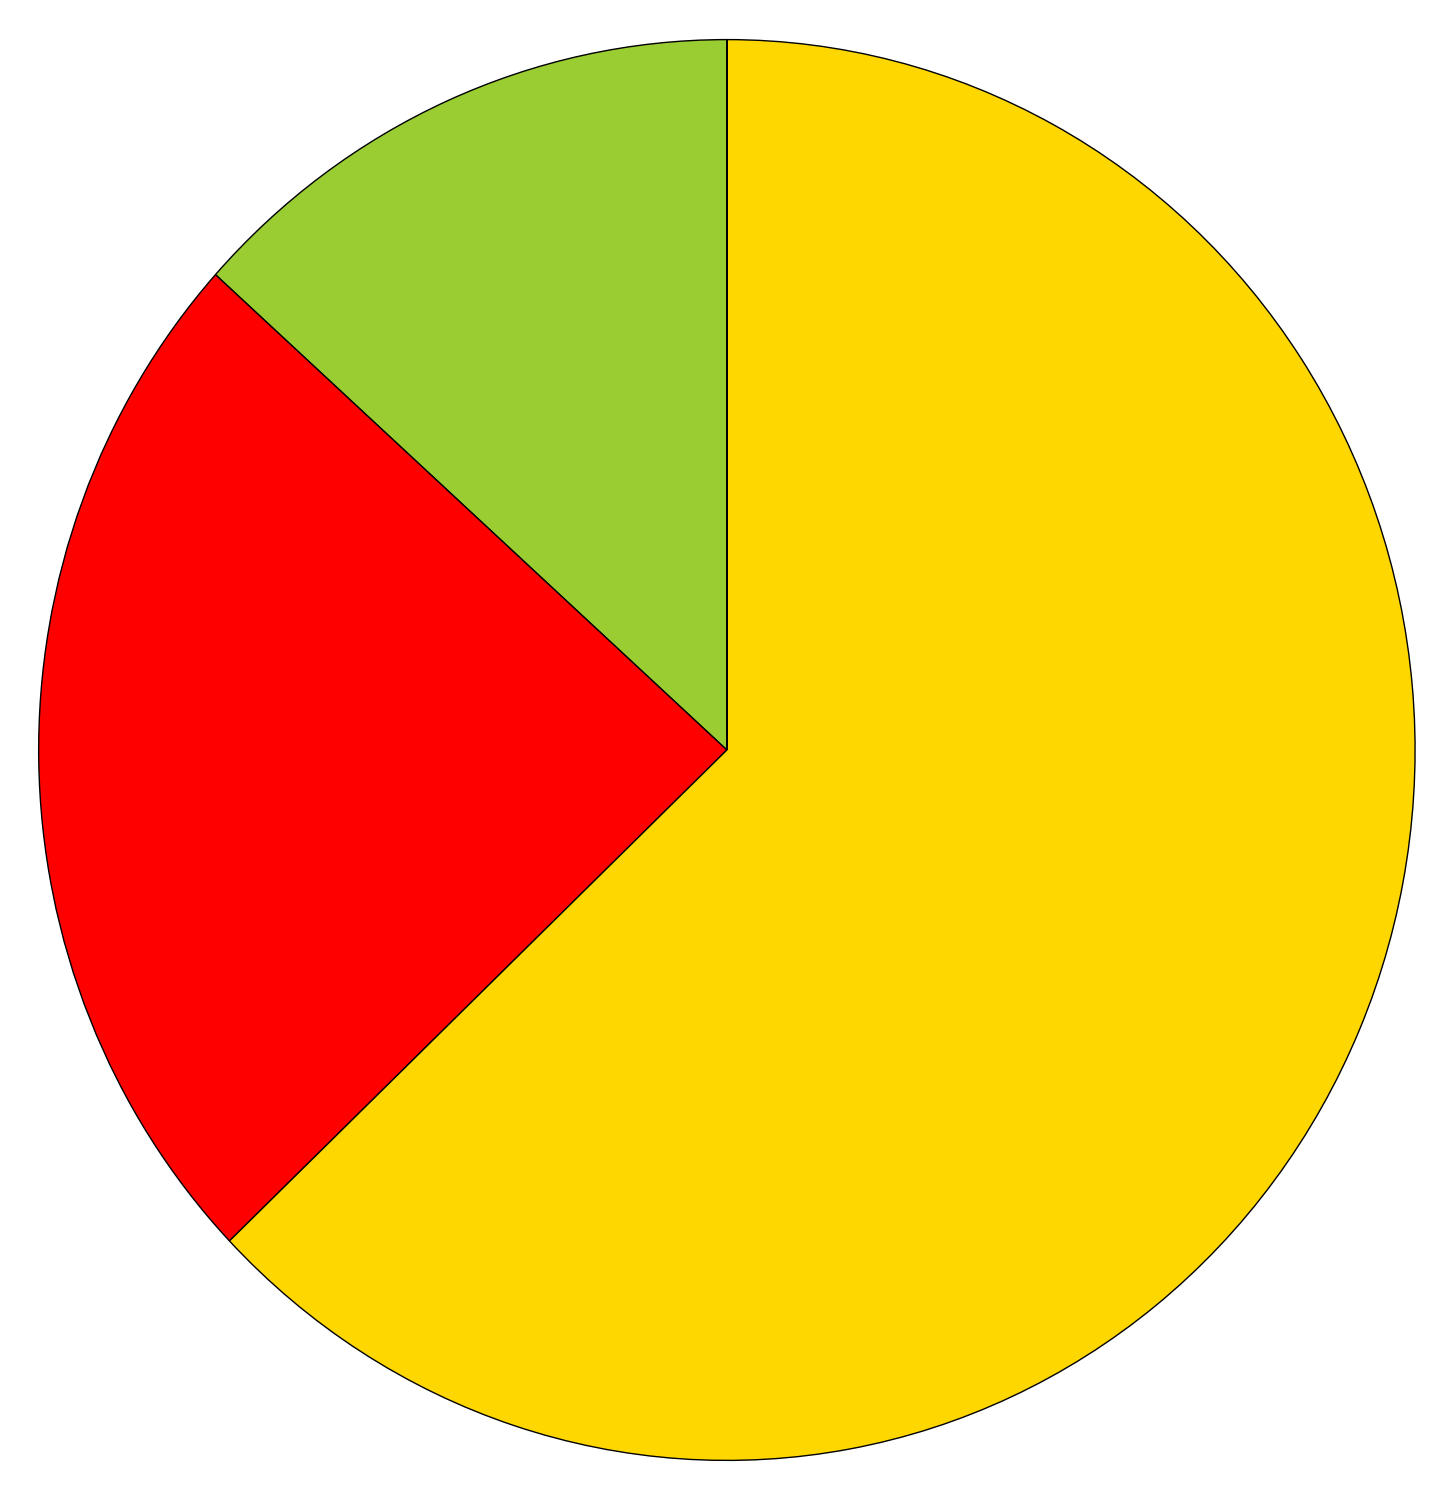
\includegraphics[width=\textwidth]{arousalEEGpearsonR}
    \caption{Pearson correlation}
  \end{subfigure}
  \hfill
  \begin{subfigure}[b]{0.3\textwidth}
    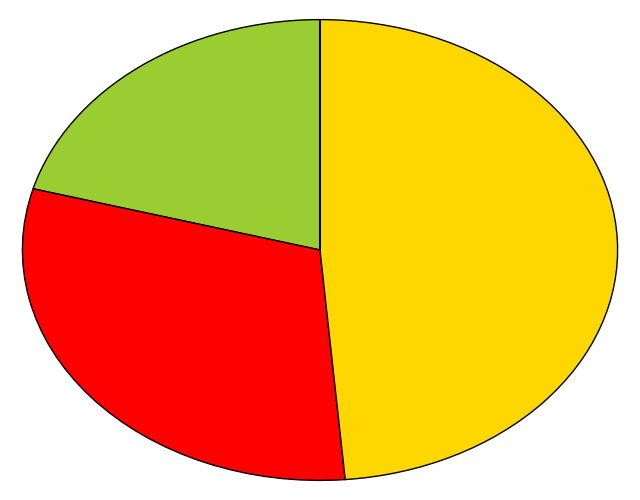
\includegraphics[width=\textwidth]{arousalEEGMutInf}
    \caption{Mutual information}
  \end{subfigure}
  \hfill
  \begin{subfigure}[b]{0.3\textwidth}
    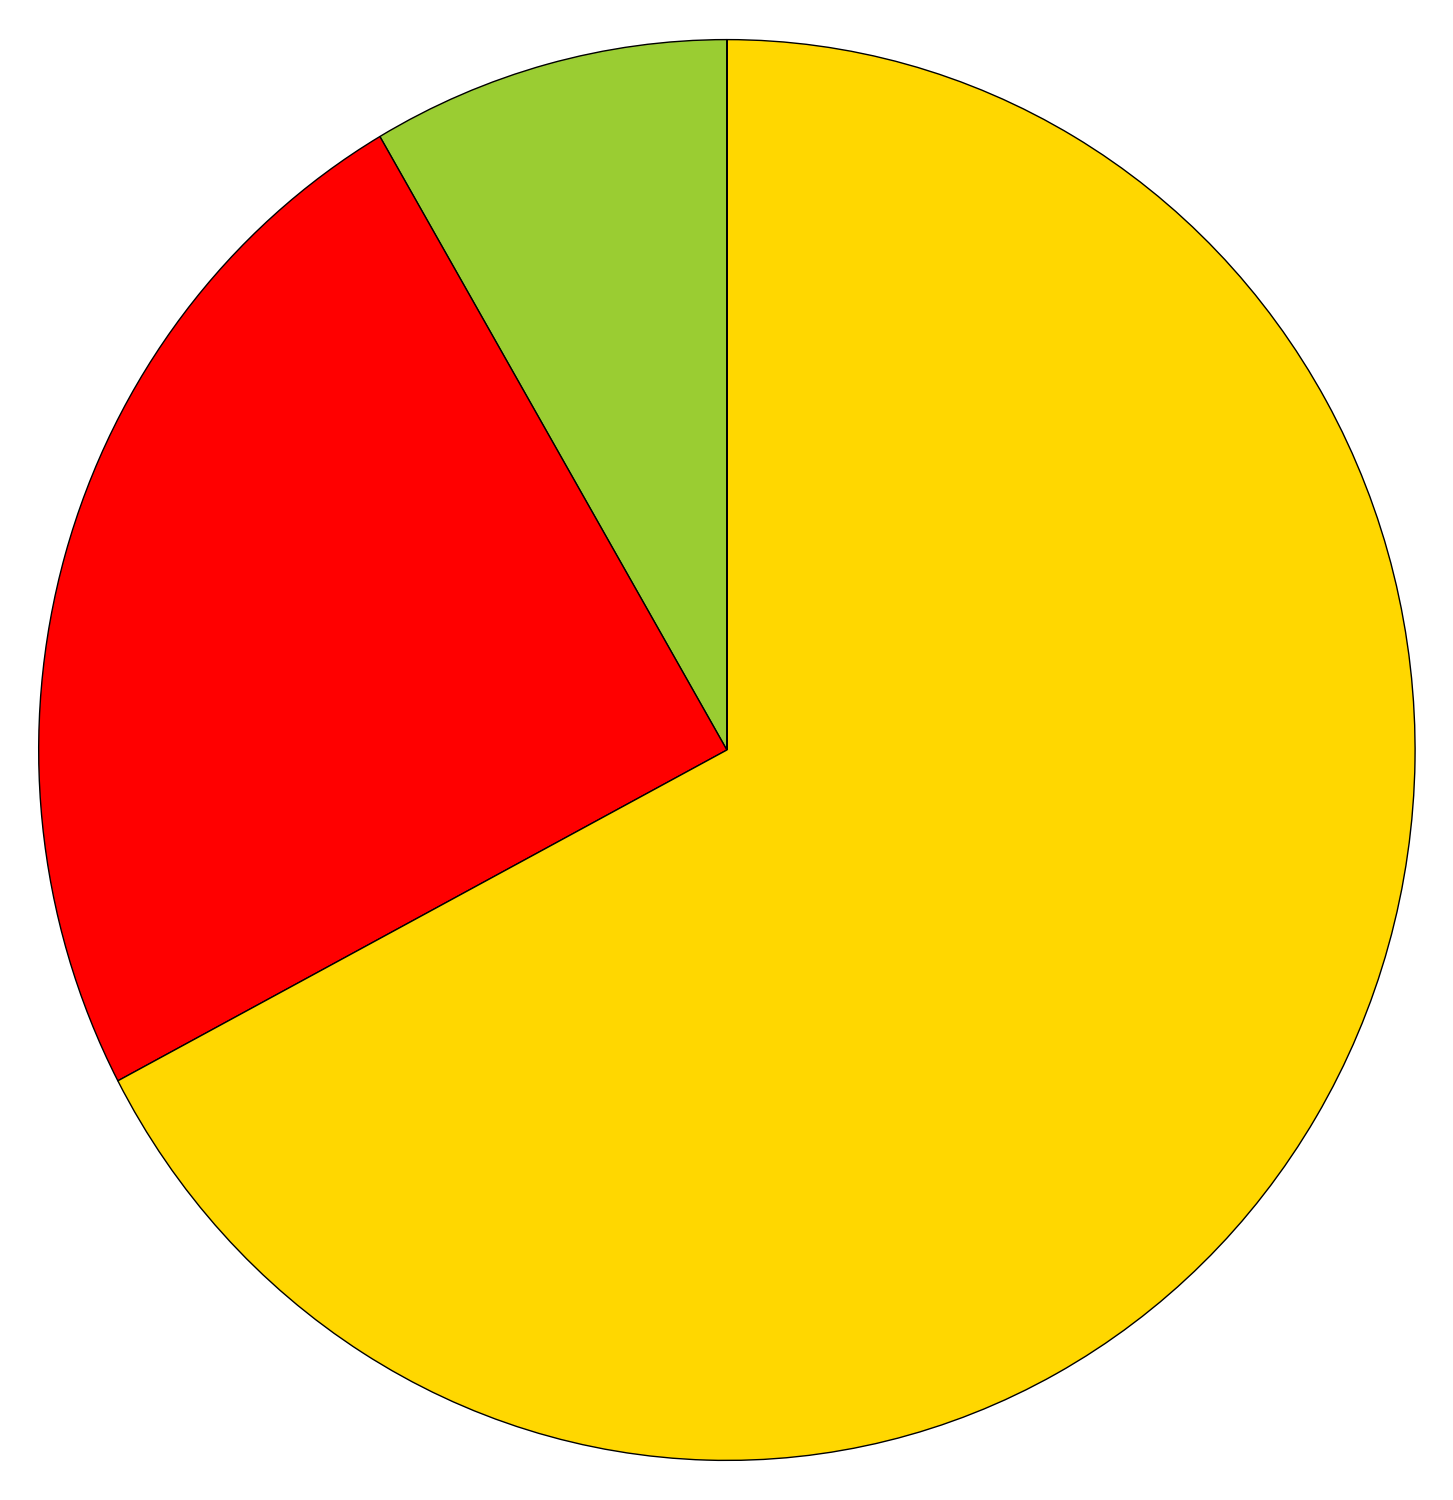
\includegraphics[width=\textwidth]{arousalEEGdCorr}
    \caption{Distance Correlation}
  \end{subfigure}
  
  \begin{subfigure}[b]{0.3\textwidth}
    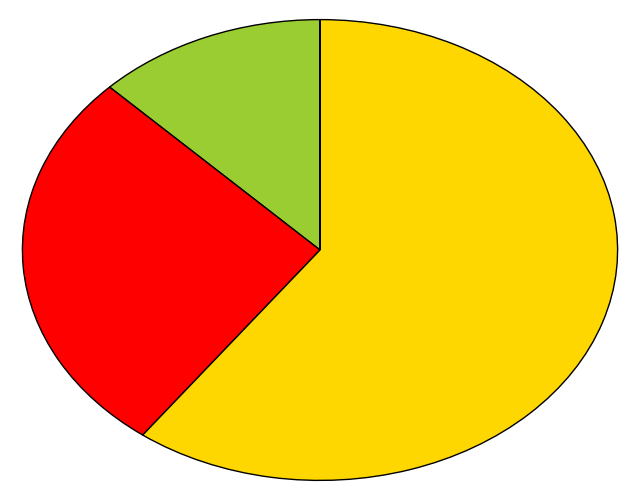
\includegraphics[width=\textwidth]{arousalEEGANOVA}
    \caption{ANOVA}
  \end{subfigure}
  \hfill
  \begin{subfigure}[b]{0.3\textwidth}
    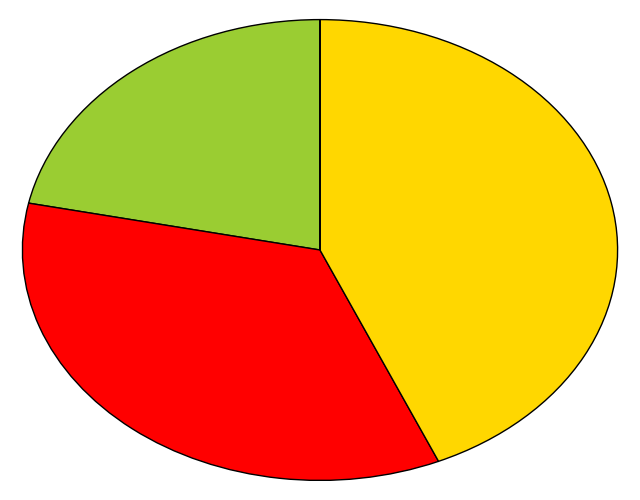
\includegraphics[width=\textwidth]{arousalEEGLR}
    \caption{Linear regression}
  \end{subfigure}
  \hfill
  \begin{subfigure}[b]{0.3\textwidth}
    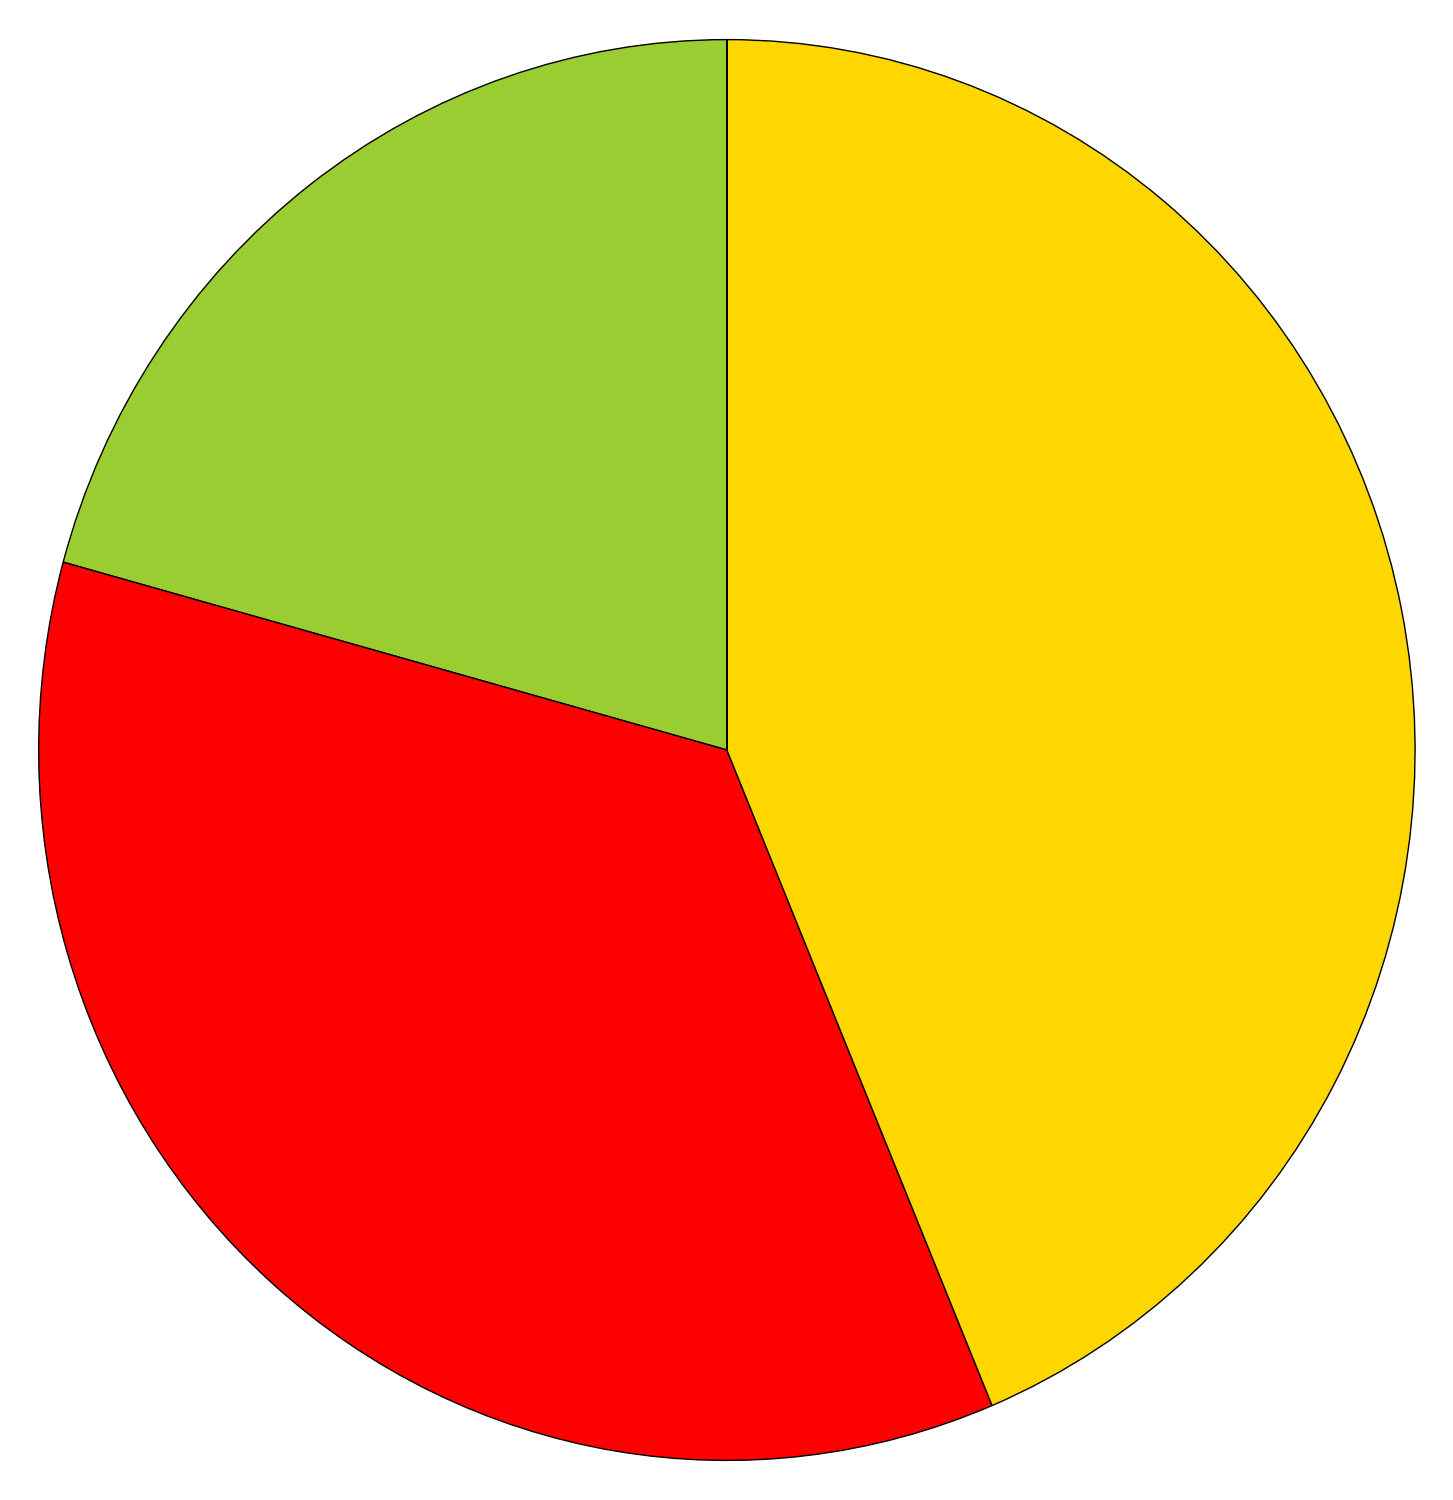
\includegraphics[width=\textwidth]{arousalEEGSVM}
    \caption{SVM}
  \end{subfigure}
  
  \begin{subfigure}[b]{0.3\textwidth}
    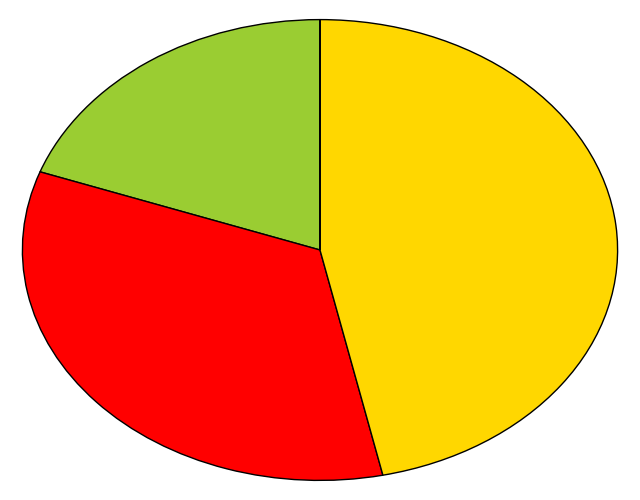
\includegraphics[width=\textwidth]{arousalEEGLDA}
    \caption{LDA}
  \end{subfigure}
  \hfill
  \begin{subfigure}[b]{0.3\textwidth}
    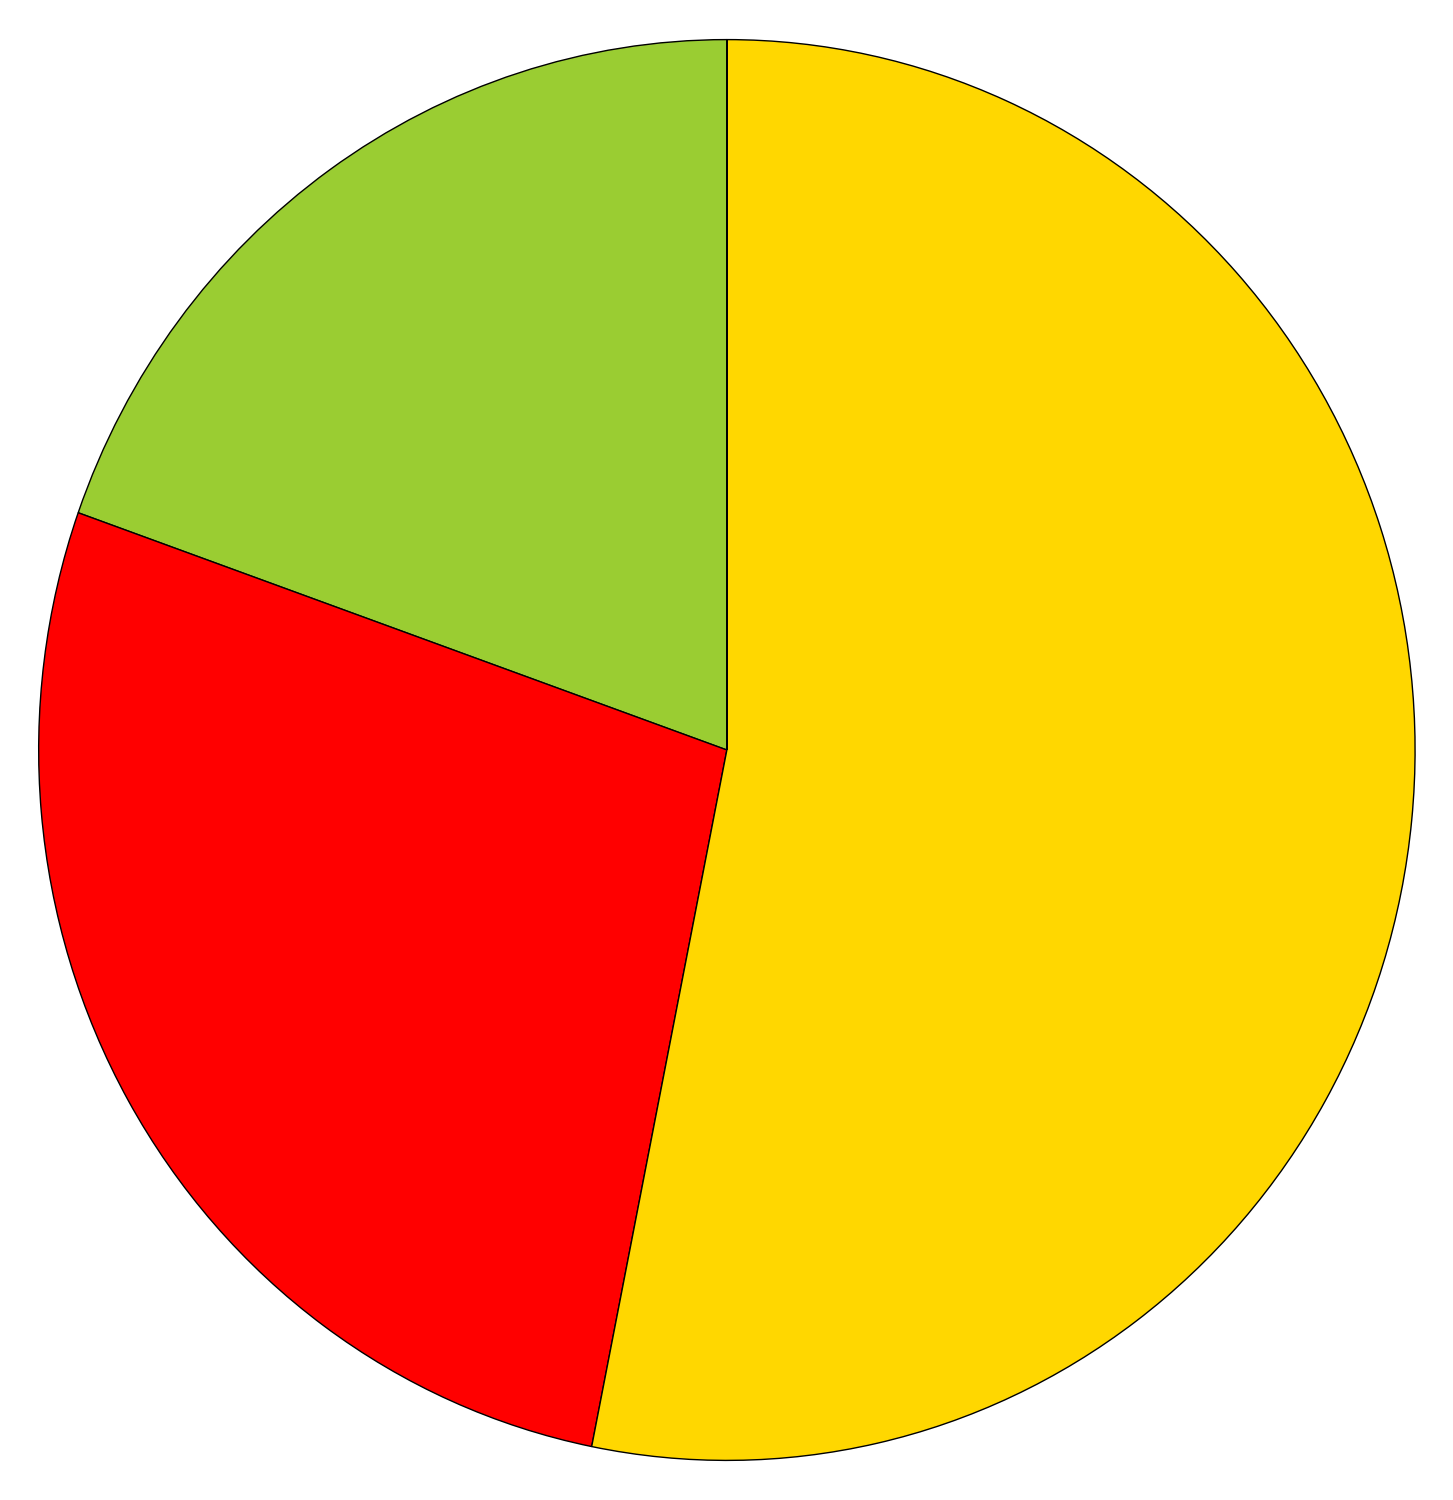
\includegraphics[width=\textwidth]{arousalEEGL1}
    \caption{Lasso regression}
  \end{subfigure}
  \hfill
  \begin{subfigure}[b]{0.3\textwidth}
    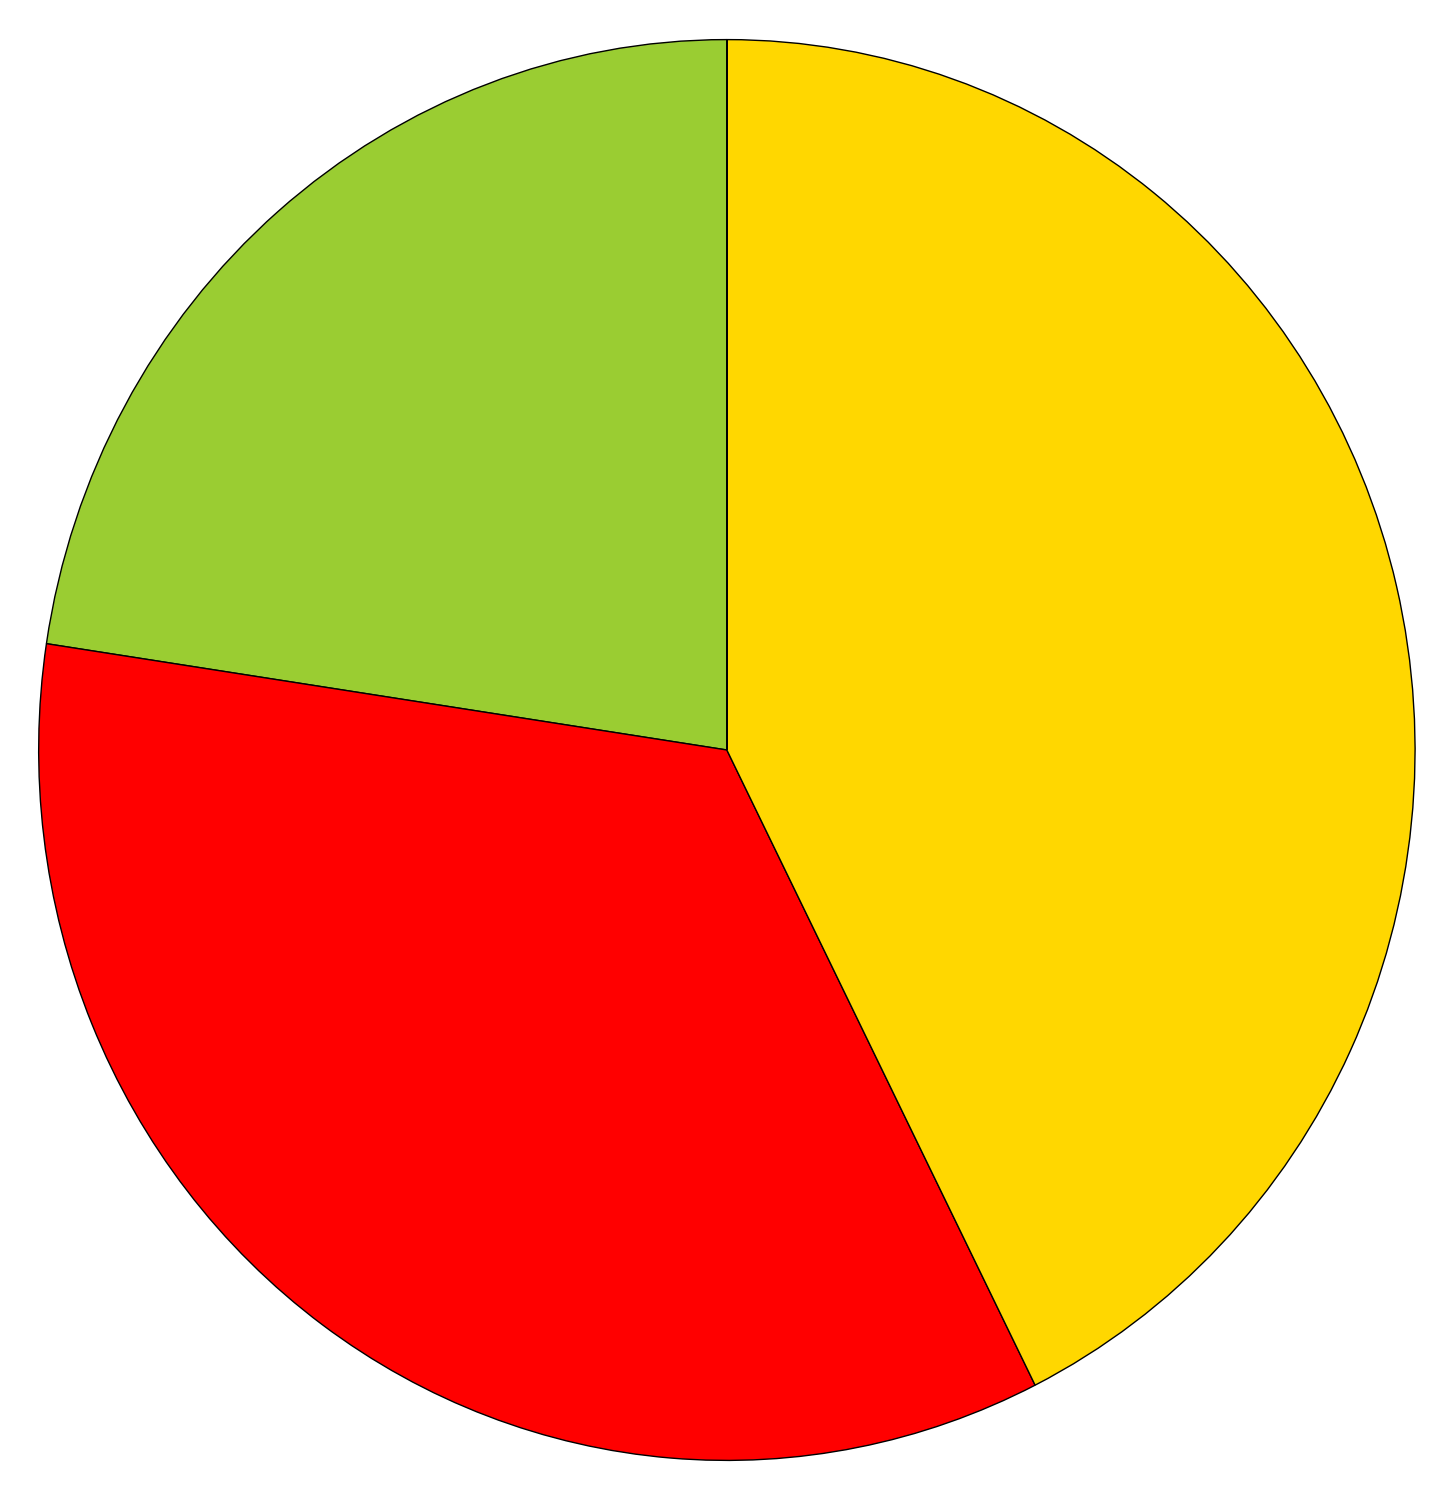
\includegraphics[width=\textwidth]{arousalEEGL2}
    \caption{Ridge regression}
  \end{subfigure}
  
  \begin{subfigure}[b]{0.3\textwidth}
    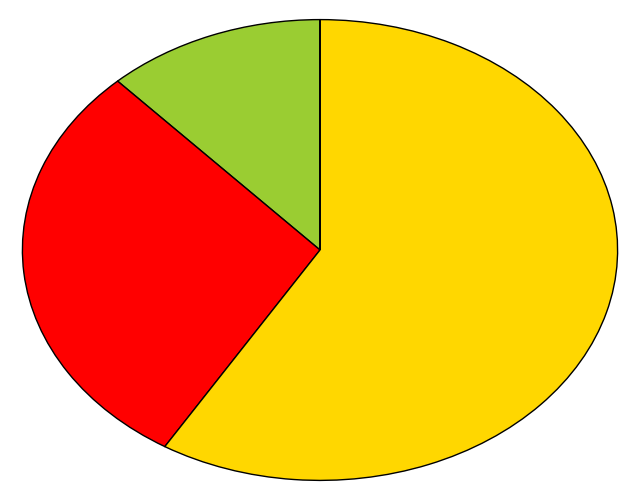
\includegraphics[width=\textwidth]{arousalEEGRF}
    \caption{Random forests}
  \end{subfigure}
  \hfill
  \begin{subfigure}[b]{0.3\textwidth}
    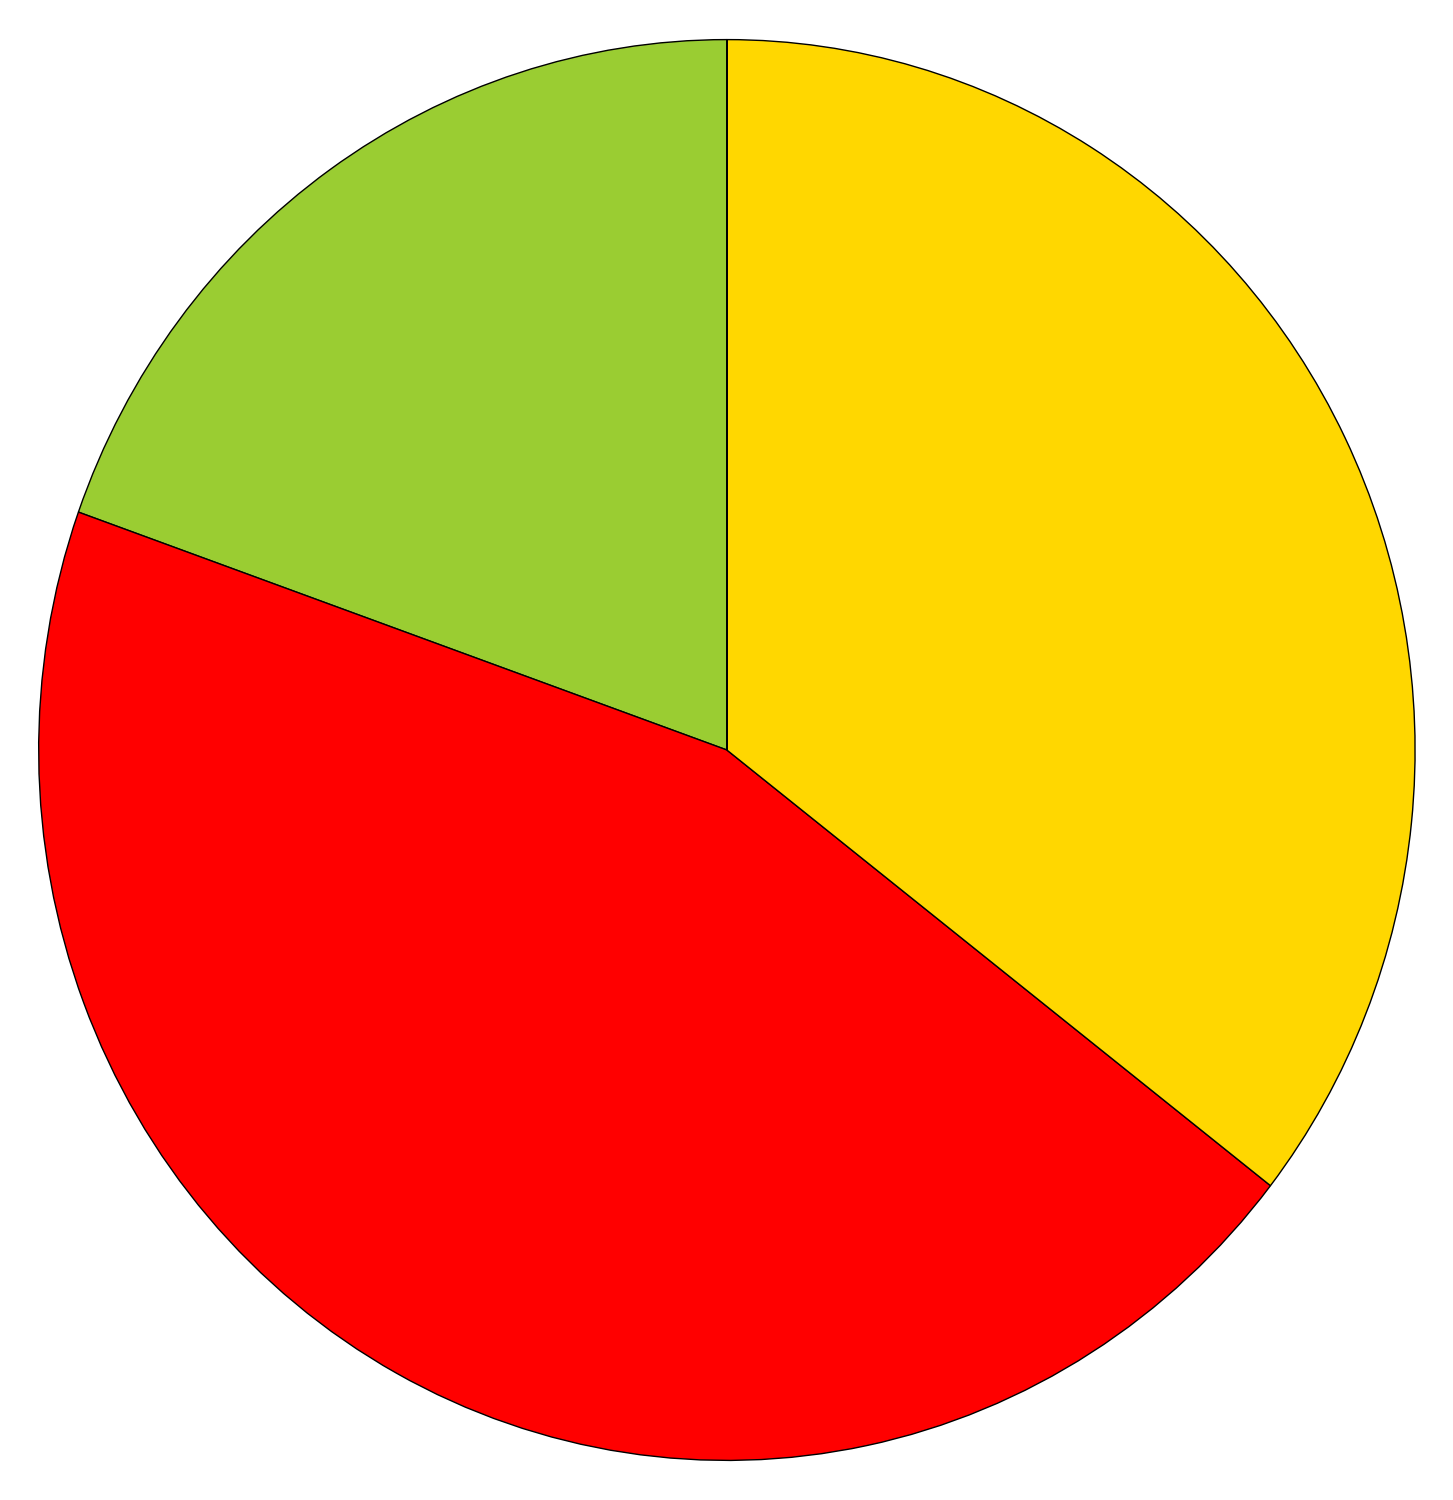
\includegraphics[width=\textwidth]{arousalEEGPCA}
    \caption{PCA}
  \end{subfigure}
  \hfill
  \begin{subfigure}[b]{0.3\textwidth}
    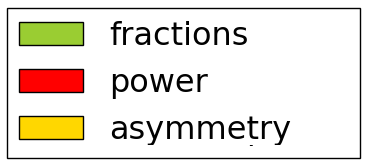
\includegraphics[width=\textwidth]{EEGlegend}
    \caption{Legend\label{arousalpiesEEGlegend}}
  \end{subfigure}
\caption{The distribution of the selected features for arousal classification of all persons combined of different feature selection methods. The feature set was limited to EEG features only.\label{arousalEEGpies}}
\end{figure}

\clearpage

\begin{figure}[!tbp]
  \centering
  \begin{subfigure}[b]{0.3\textwidth}
    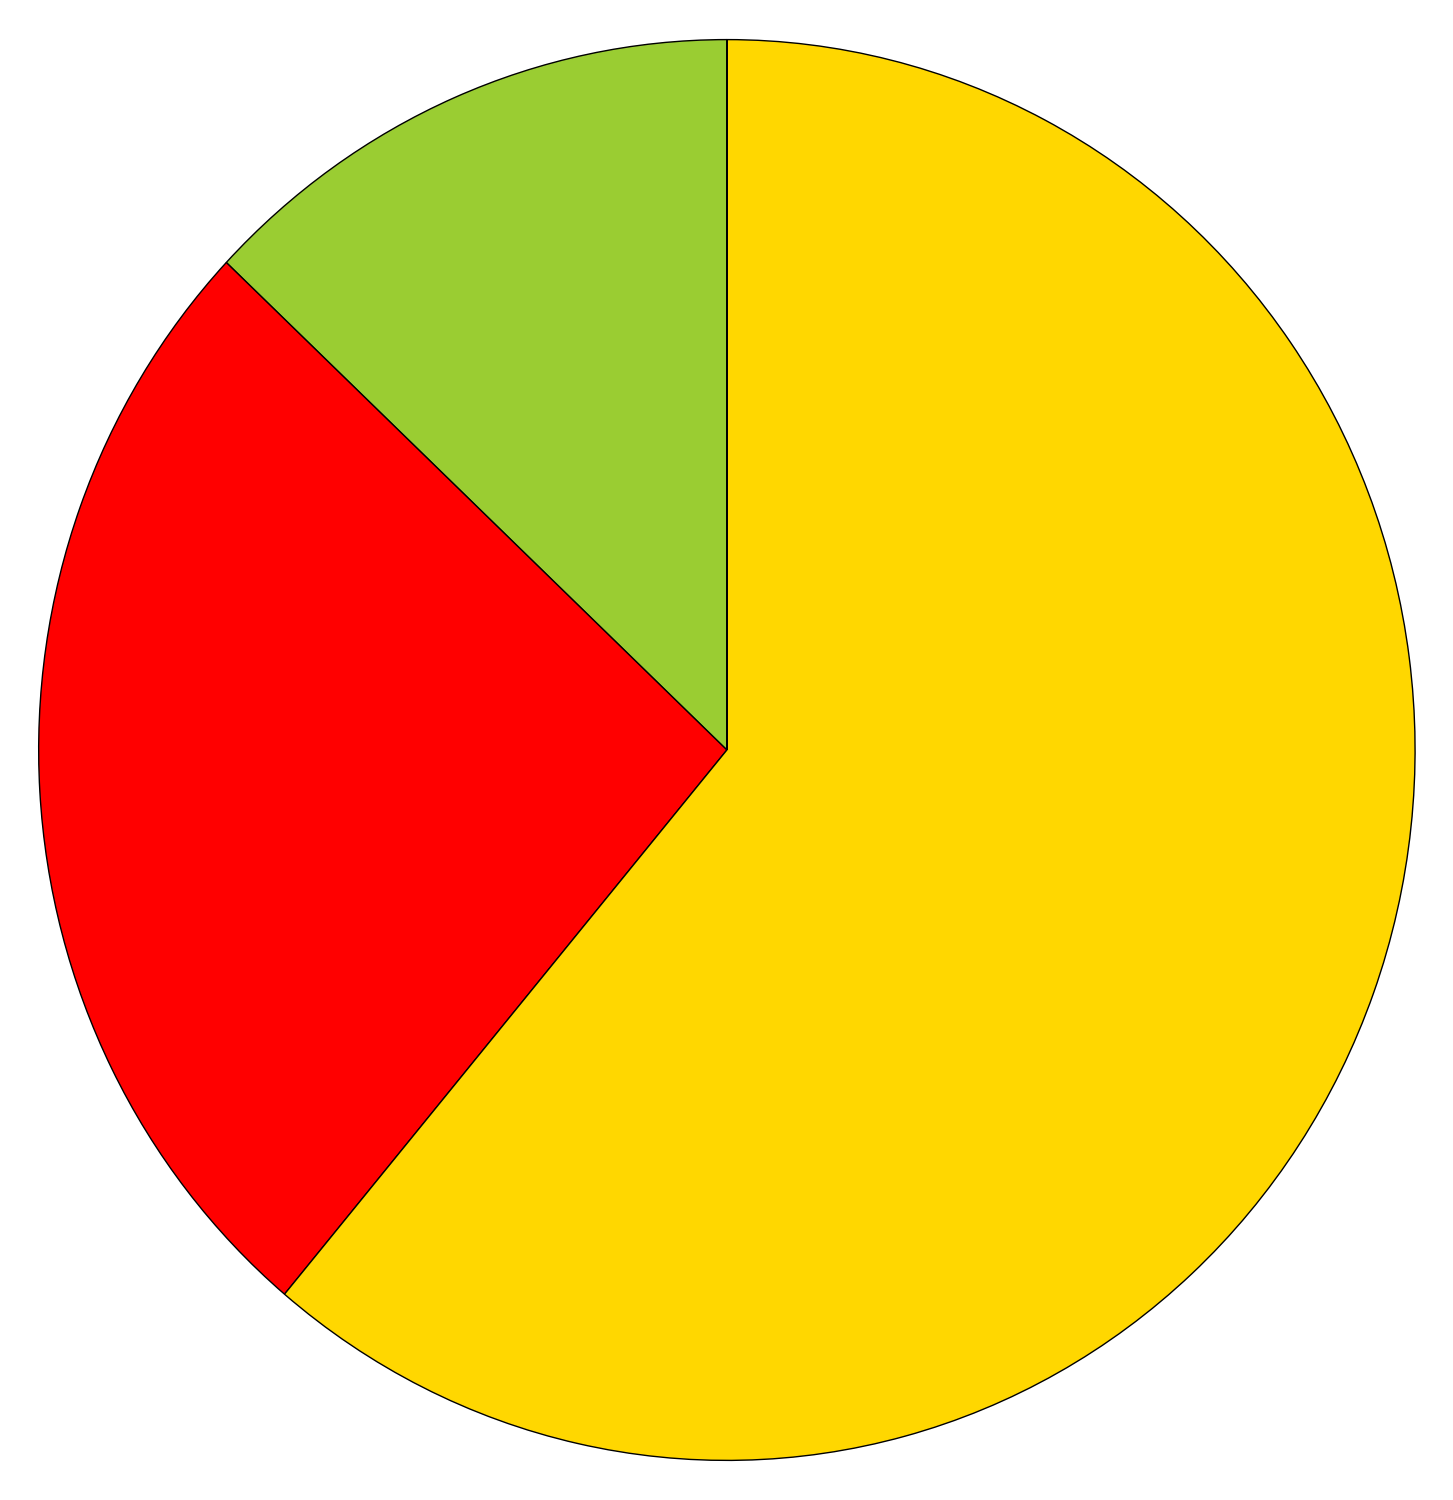
\includegraphics[width=\textwidth]{valenceEEGpearsonR}
    \caption{Pearson correlation}
  \end{subfigure}
  \hfill
  \begin{subfigure}[b]{0.3\textwidth}
    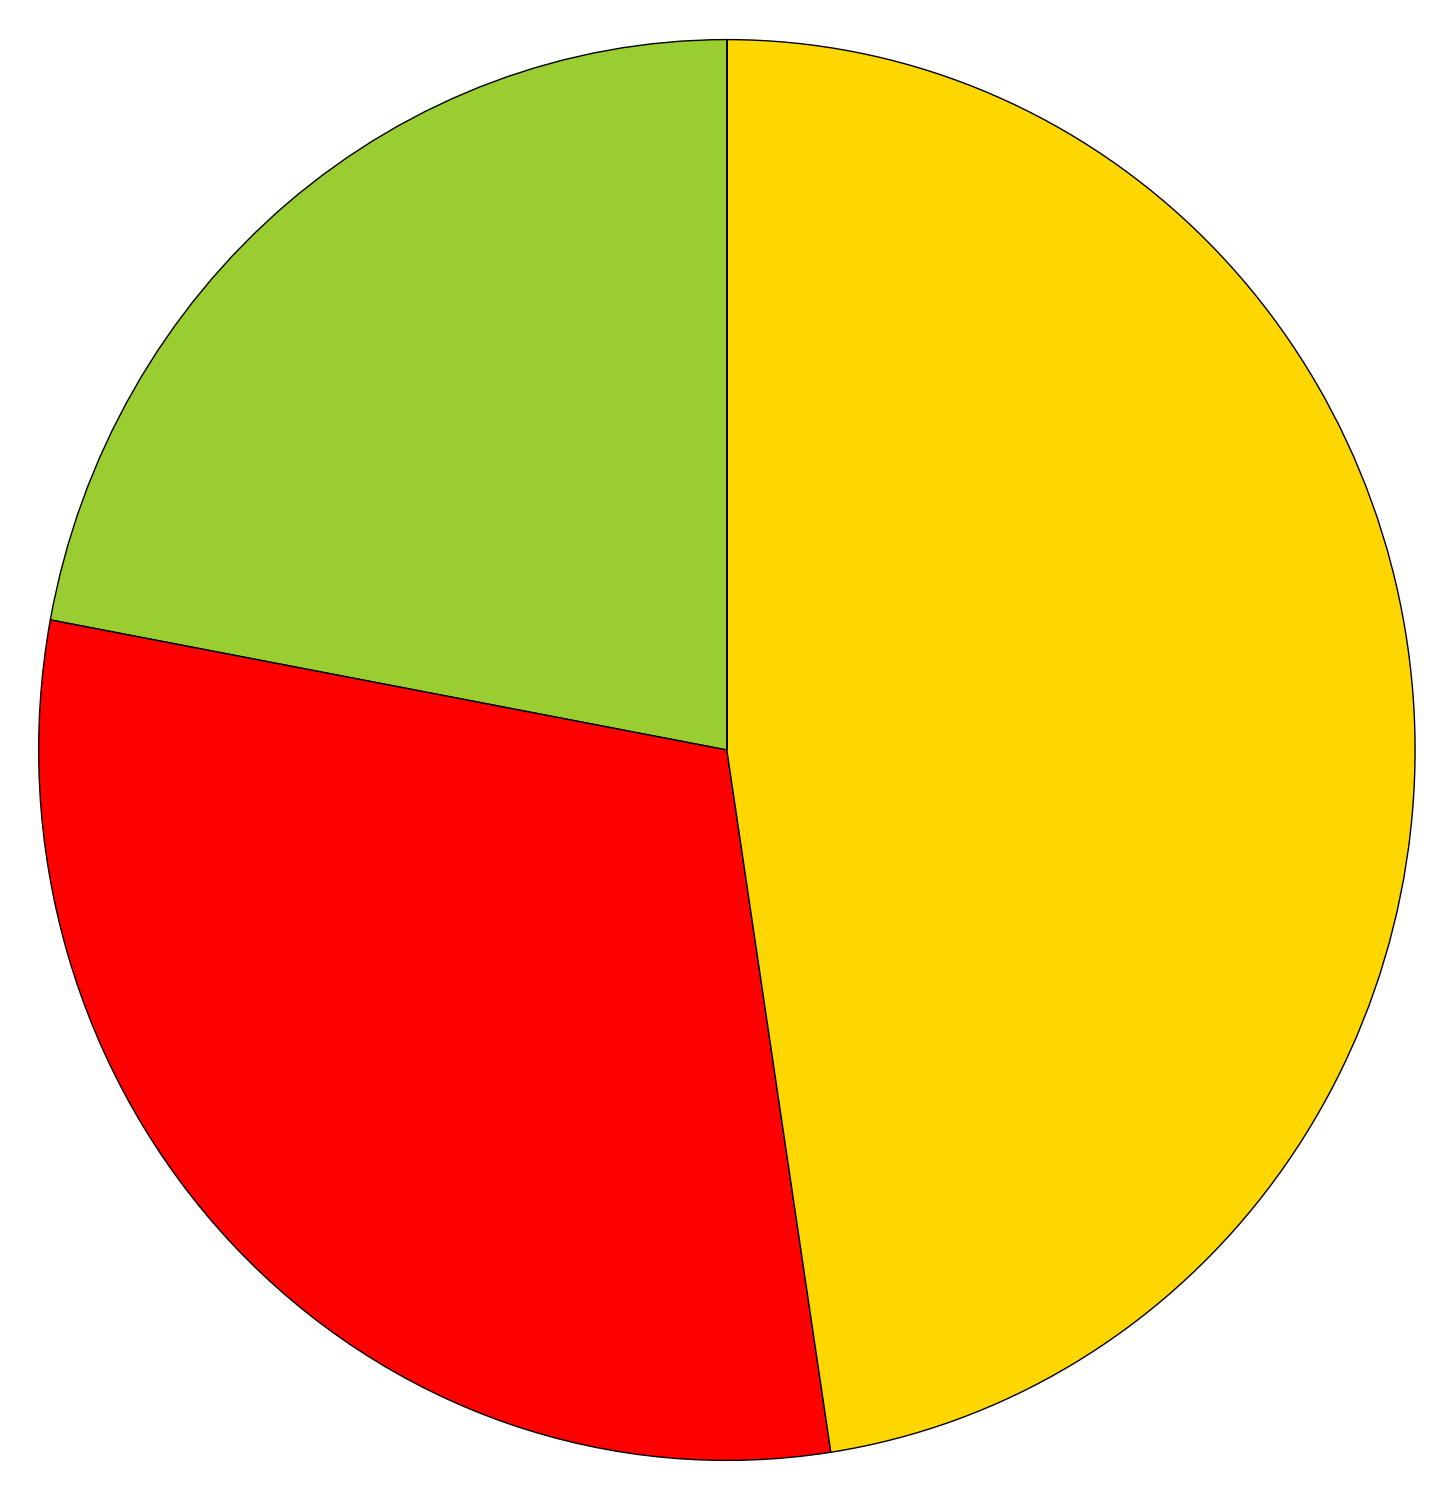
\includegraphics[width=\textwidth]{valenceEEGMutInf}
    \caption{Mutual information}
  \end{subfigure}
  \hfill
  \begin{subfigure}[b]{0.3\textwidth}
    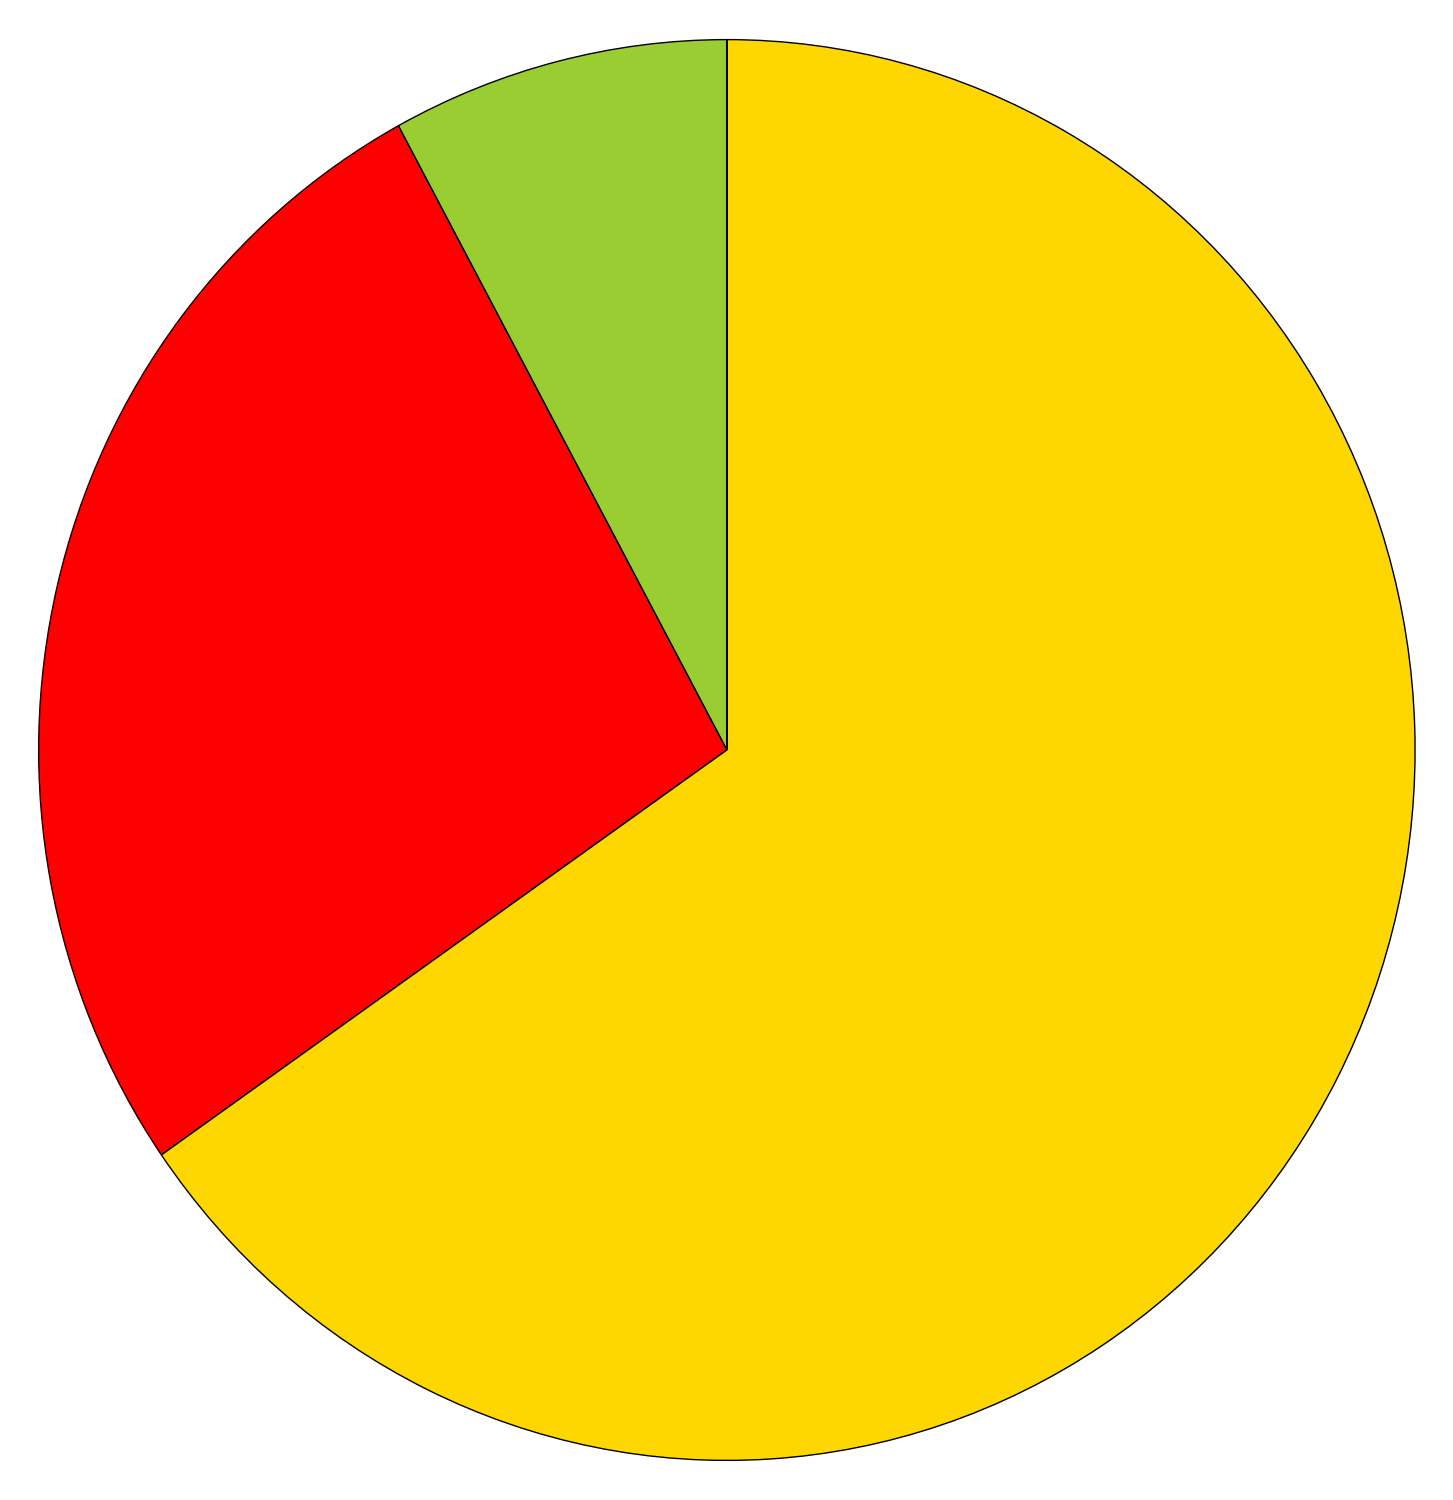
\includegraphics[width=\textwidth]{valenceEEGdCorr}
    \caption{Distance Correlation}
  \end{subfigure}
  
  \begin{subfigure}[b]{0.3\textwidth}
    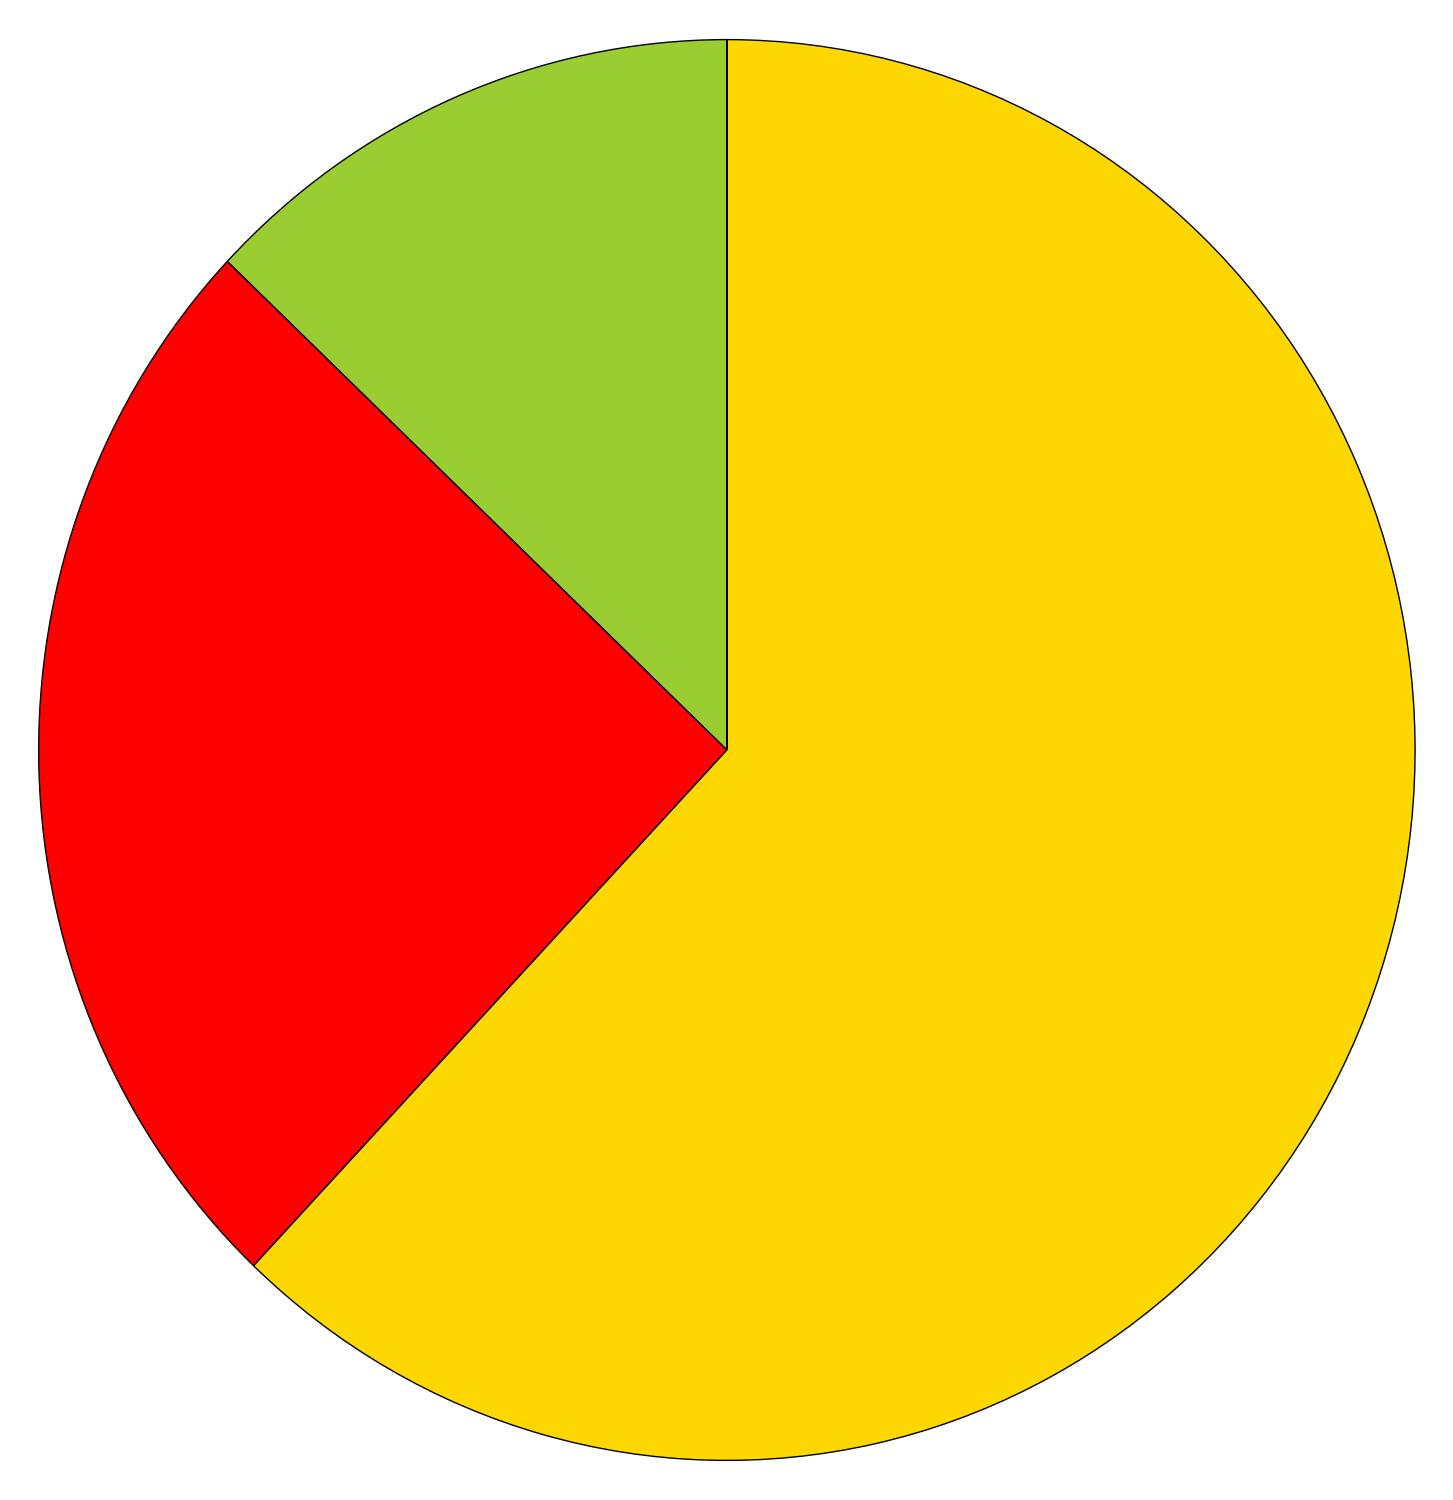
\includegraphics[width=\textwidth]{valenceEEGANOVA}
    \caption{ANOVA}
  \end{subfigure}
  \hfill
  \begin{subfigure}[b]{0.3\textwidth}
    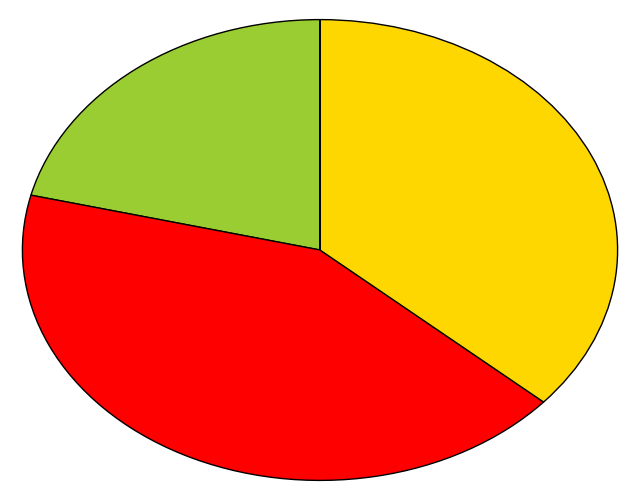
\includegraphics[width=\textwidth]{valenceEEGLR}
    \caption{Linear regression}
  \end{subfigure}
  \hfill
  \begin{subfigure}[b]{0.3\textwidth}
    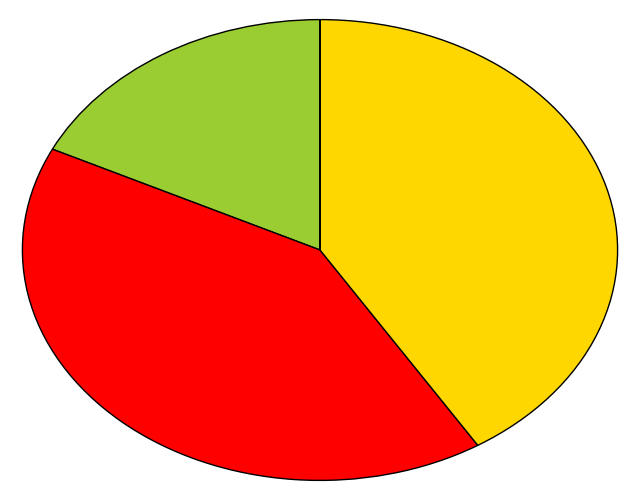
\includegraphics[width=\textwidth]{valenceEEGSVM}
    \caption{SVM}
  \end{subfigure}
  
  \begin{subfigure}[b]{0.3\textwidth}
    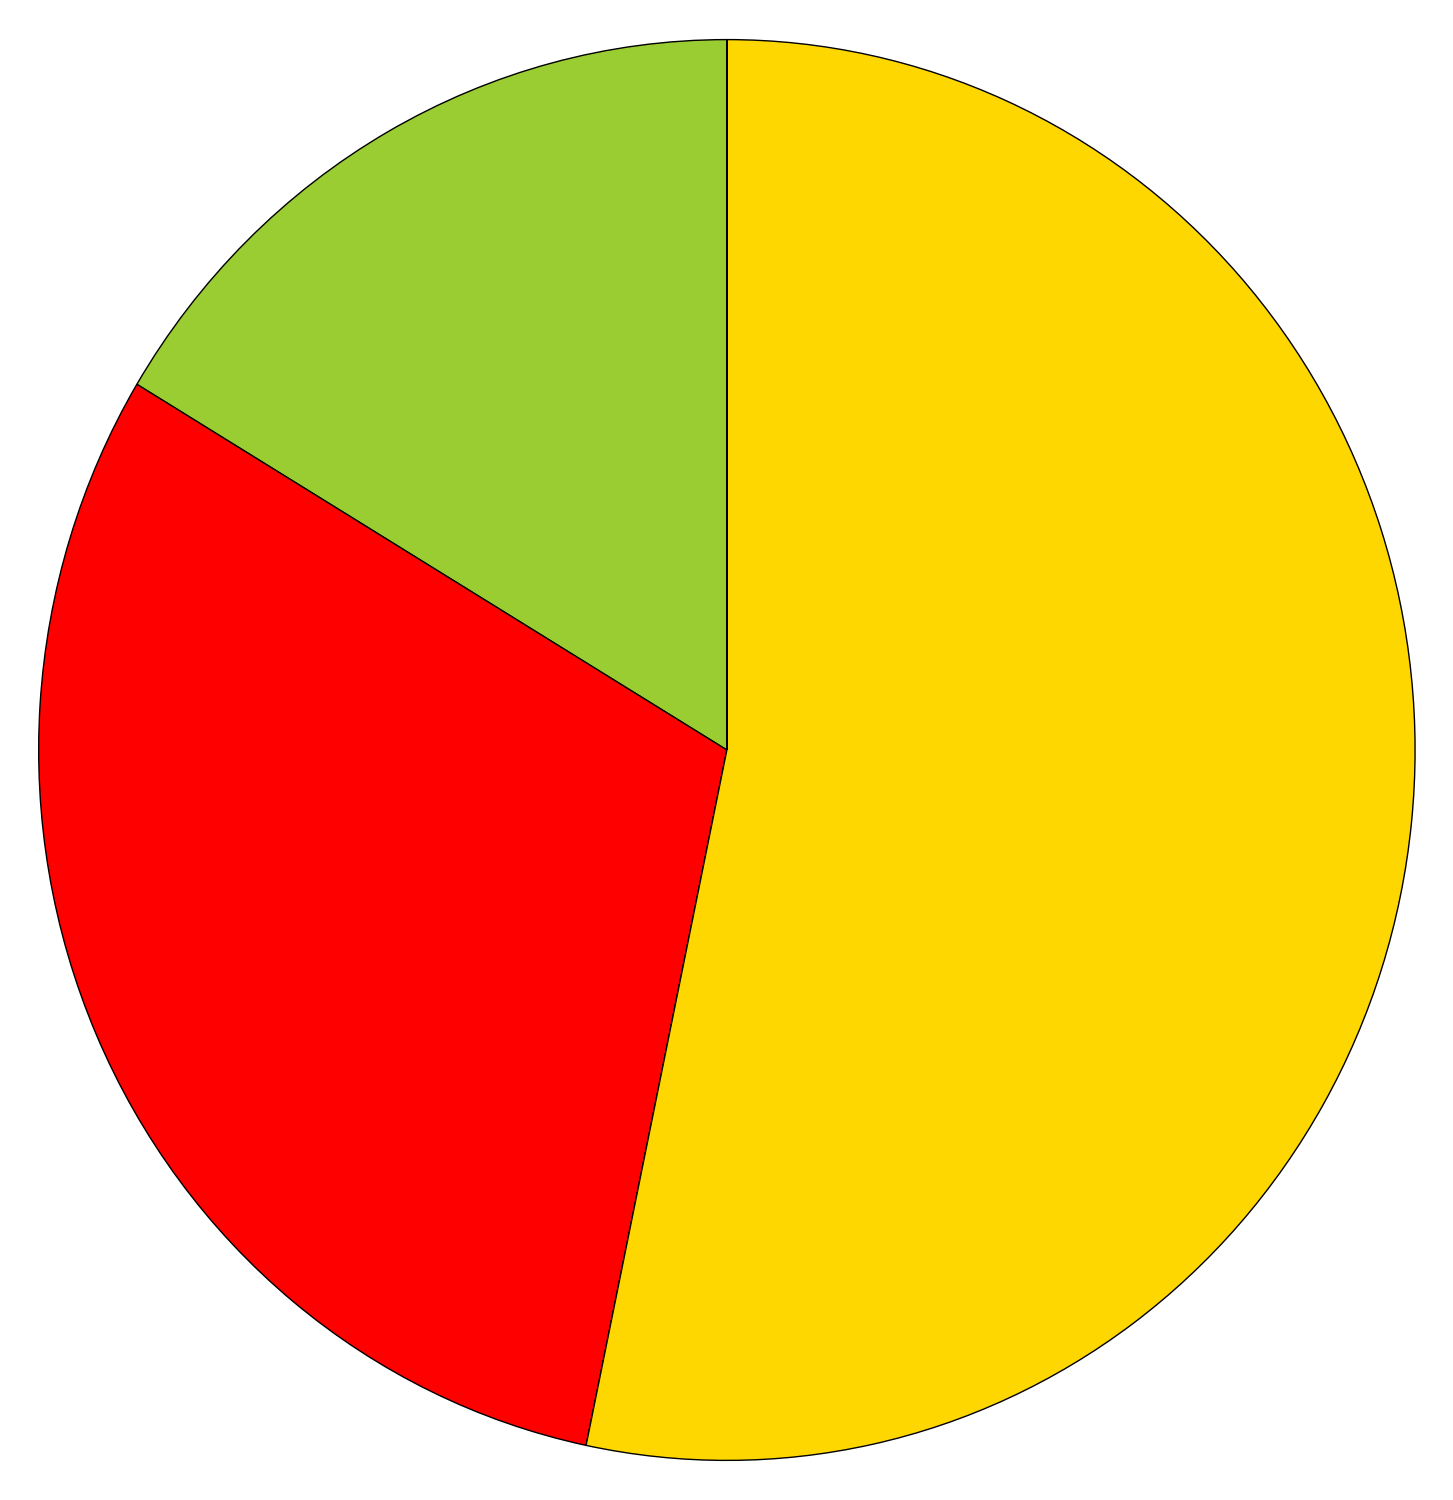
\includegraphics[width=\textwidth]{valenceEEGLDA}
    \caption{LDA}
  \end{subfigure}
  \hfill
  \begin{subfigure}[b]{0.3\textwidth}
    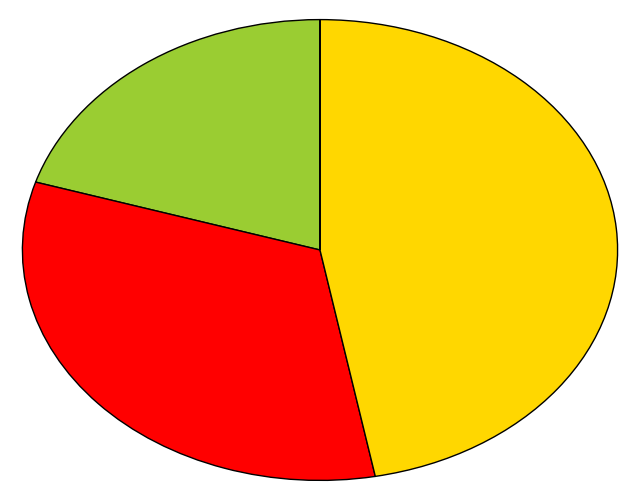
\includegraphics[width=\textwidth]{valenceEEGL1}
    \caption{Lasso regression}
  \end{subfigure}
  \hfill
  \begin{subfigure}[b]{0.3\textwidth}
    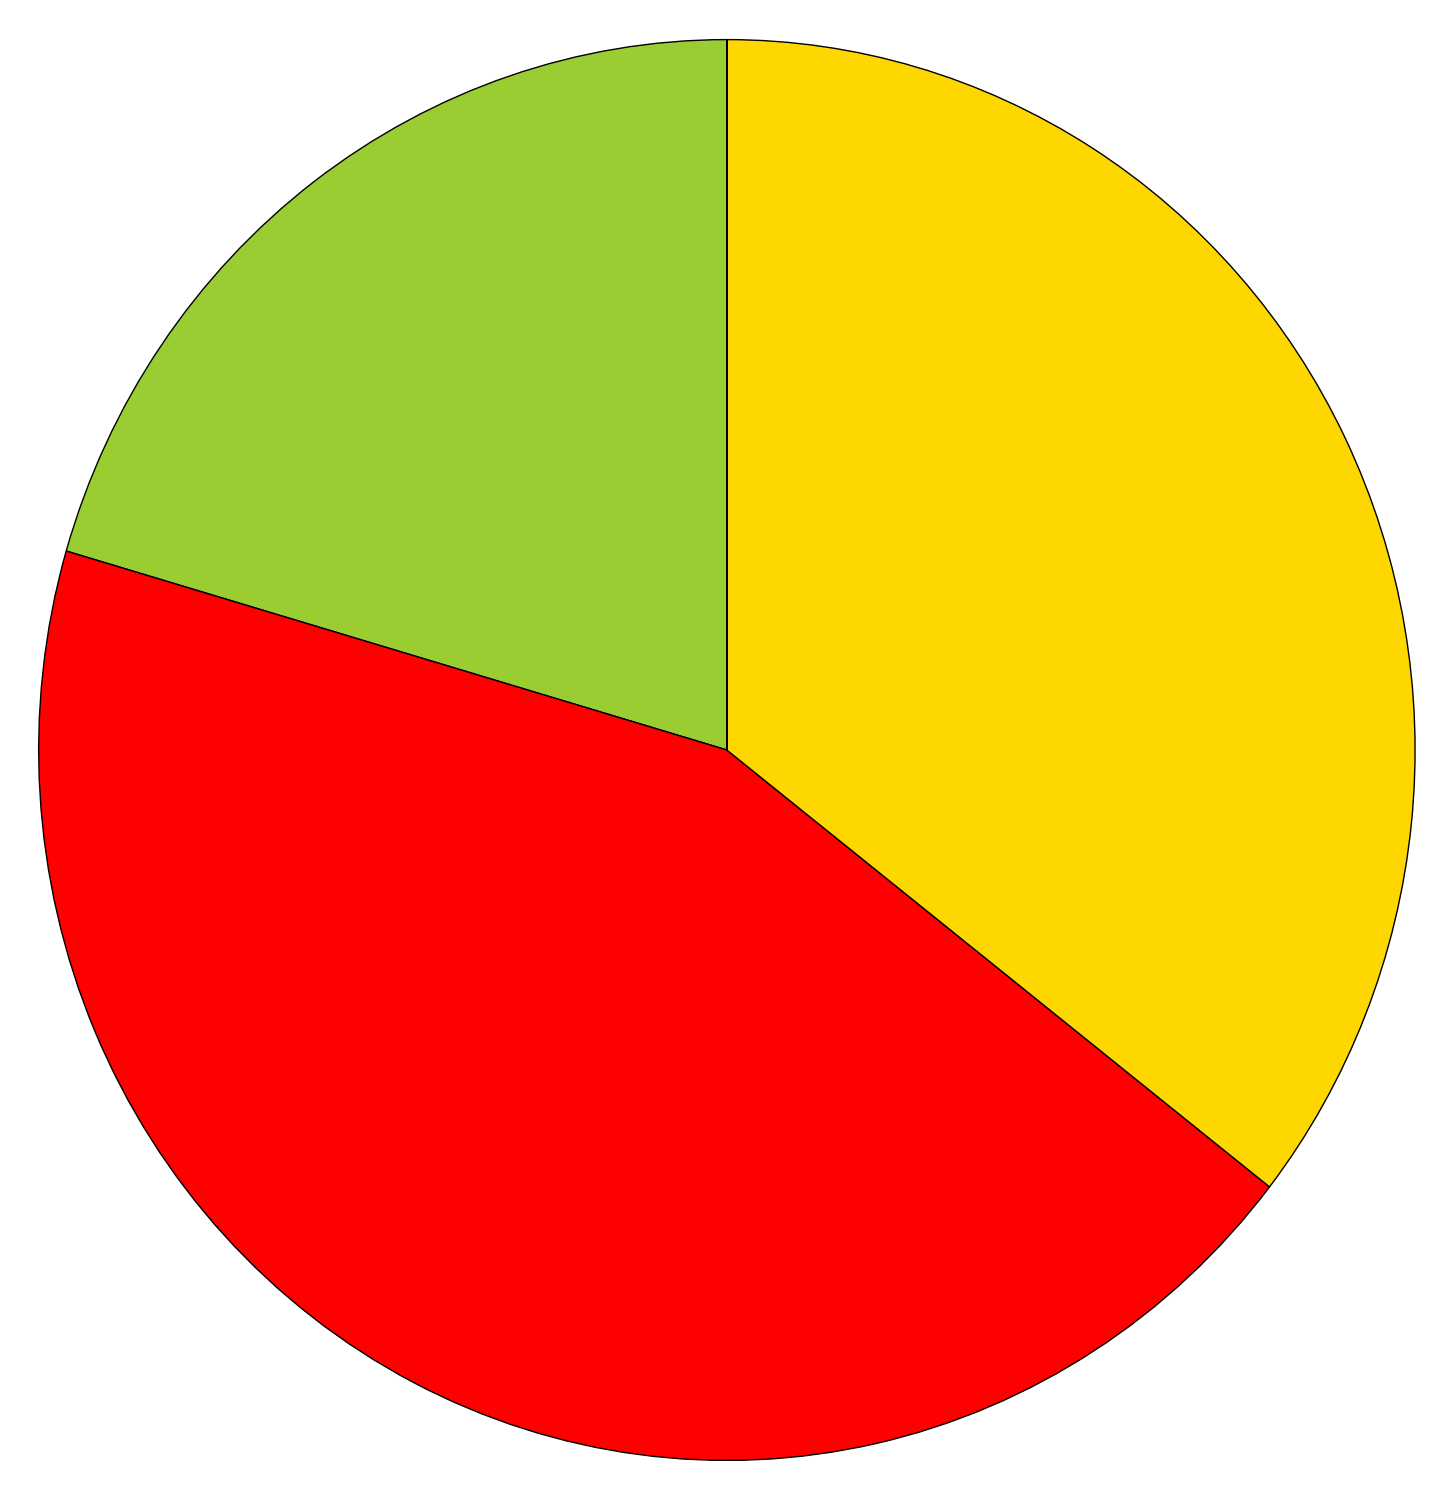
\includegraphics[width=\textwidth]{valenceEEGL2}
    \caption{Ridge regression}
  \end{subfigure}
  
  \begin{subfigure}[b]{0.3\textwidth}
    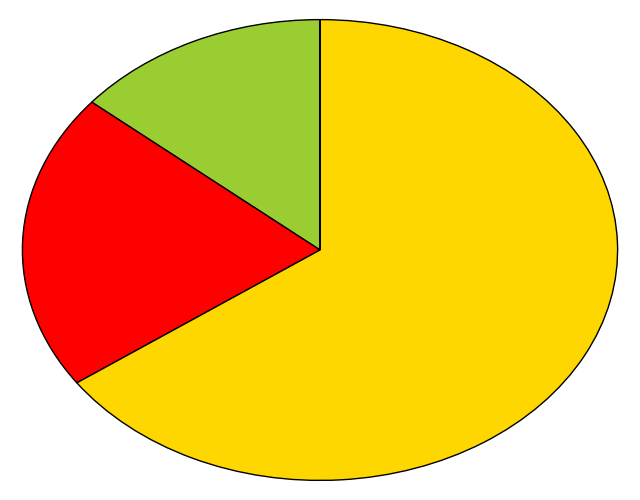
\includegraphics[width=\textwidth]{valenceEEGRF}
    \caption{Random forests}
  \end{subfigure}
  \hfill
  \begin{subfigure}[b]{0.3\textwidth}
    \includegraphics[width=\textwidth]{valenceEEGPCA}
    \caption{PCA}
  \end{subfigure}
  \hfill
  \begin{subfigure}[b]{0.3\textwidth}
    \includegraphics[width=\textwidth]{EEGlegend}
    \caption{Legend\label{valencepiesEEGlegend}}
  \end{subfigure}
  \caption{The distribution of the selected features for valence classification of all persons combined of different feature selection methods. The feature set was limited to EEG features only.\label{valenceEEGpies}}
\end{figure}
\clearpage

\begin{figure}[!tbp]
  \centering
  \begin{subfigure}[b]{0.3\textwidth}
    \includegraphics[width=\textwidth]{arousalnon-EEGpearsonR}
    \caption{Pearson correlation}
  \end{subfigure}
  \hfill
  \begin{subfigure}[b]{0.3\textwidth}
    \includegraphics[width=\textwidth]{arousalnon-EEGMutInf}
    \caption{Mutual information}
  \end{subfigure}
  \hfill
  \begin{subfigure}[b]{0.3\textwidth}
    \includegraphics[width=\textwidth]{arousalnon-EEGdCorr}
    \caption{Distance Correlation}
  \end{subfigure}
  
  \begin{subfigure}[b]{0.3\textwidth}
    \includegraphics[width=\textwidth]{arousalnon-EEGANOVA}
    \caption{ANOVA}
  \end{subfigure}
  \hfill
  \begin{subfigure}[b]{0.3\textwidth}
    \includegraphics[width=\textwidth]{arousalnon-EEGLR}
    \caption{Linear regression}
  \end{subfigure}
  \hfill
  \begin{subfigure}[b]{0.3\textwidth}
    \includegraphics[width=\textwidth]{arousalnon-EEGSVM}
    \caption{SVM}
  \end{subfigure}
  
  \begin{subfigure}[b]{0.3\textwidth}
    \includegraphics[width=\textwidth]{arousalnon-EEGLDA}
    \caption{LDA}
  \end{subfigure}
  \hfill
  \begin{subfigure}[b]{0.3\textwidth}
    \includegraphics[width=\textwidth]{arousalnon-EEGL1}
    \caption{Lasso regression}
  \end{subfigure}
  \hfill
  \begin{subfigure}[b]{0.3\textwidth}
    \includegraphics[width=\textwidth]{arousalnon-EEGL2}
    \caption{Ridge regression}
  \end{subfigure}
  
  \begin{subfigure}[b]{0.3\textwidth}
    \includegraphics[width=\textwidth]{arousalnon-EEGRF}
    \caption{Random forests}
  \end{subfigure}
  \hfill
  \begin{subfigure}[b]{0.3\textwidth}
    \includegraphics[width=\textwidth]{arousalnon-EEGPCA}
    \caption{PCA}
  \end{subfigure}
  \hfill
  \begin{subfigure}[b]{0.3\textwidth}
    \includegraphics[width=\textwidth]{non-EEGlegend}
    \caption{Legend\label{arousalpiesnon-EEGlegend}}
  \end{subfigure}    
\caption{The distribution of the selected features for arousal classification of all persons combined of different feature selection methods. The feature set was limited to non-EEG features only.\label{arousalnon-EEGpies}}
\end{figure}

\clearpage

\begin{figure}[!tbp]
  \centering
  \begin{subfigure}[b]{0.3\textwidth}
    \includegraphics[width=\textwidth]{valencenon-EEGpearsonR}
    \caption{Pearson correlation}
  \end{subfigure}
  \hfill
  \begin{subfigure}[b]{0.3\textwidth}
    \includegraphics[width=\textwidth]{valencenon-EEGMutInf}
    \caption{Mutual information}
  \end{subfigure}
  \hfill
  \begin{subfigure}[b]{0.3\textwidth}
    \includegraphics[width=\textwidth]{valencenon-EEGdCorr}
    \caption{Distance Correlation}
  \end{subfigure}
  
  \begin{subfigure}[b]{0.3\textwidth}
    \includegraphics[width=\textwidth]{valencenon-EEGANOVA}
    \caption{ANOVA}
  \end{subfigure}
  \hfill
  \begin{subfigure}[b]{0.3\textwidth}
    \includegraphics[width=\textwidth]{valencenon-EEGLR}
    \caption{Linear regression}
  \end{subfigure}
  \hfill
  \begin{subfigure}[b]{0.3\textwidth}
    \includegraphics[width=\textwidth]{valencenon-EEGSVM}
    \caption{SVM}
  \end{subfigure}
  
  \begin{subfigure}[b]{0.3\textwidth}
    \includegraphics[width=\textwidth]{valencenon-EEGLDA}
    \caption{LDA}
  \end{subfigure}
  \hfill
  \begin{subfigure}[b]{0.3\textwidth}
    \includegraphics[width=\textwidth]{valencenon-EEGL1}
    \caption{Lasso regression}
  \end{subfigure}
  \hfill
  \begin{subfigure}[b]{0.3\textwidth}
    \includegraphics[width=\textwidth]{valencenon-EEGL2}
    \caption{Ridge regression}
  \end{subfigure}
  
  \begin{subfigure}[b]{0.3\textwidth}
    \includegraphics[width=\textwidth]{valencenon-EEGRF}
    \caption{Random forests}
  \end{subfigure}
  \hfill
  \begin{subfigure}[b]{0.3\textwidth}
    \includegraphics[width=\textwidth]{valencenon-EEGPCA}
    \caption{PCA}
  \end{subfigure}
  \hfill
  \begin{subfigure}[b]{0.3\textwidth}
    \includegraphics[width=\textwidth]{non-EEGlegend}
    \caption{Legend\label{valencepiesnon-EEGlegend}}
  \end{subfigure}
  \caption{The distribution of the selected features for valence classification of all persons combined of different feature selection methods. The feature set was limited to non-EEG features only.\label{valencenon-EEGpies}}
\end{figure}
\clearpage

\section{Important EEG channels}

Another component of this work is to dig into the EEG features and find out which channels are most important. This was done by taking the Random forest as a feature selection model and looking at the models that were build. By simply counting the occurrences of different EEG channels in these models, pie charts were constructed. This was done for both valence and arousal. The results are displayed in Figure\ref{arousalchannel} for arousal and Figure \ref{valencechannel} for valence.

\begin{figure}[H]
\centering
  \begin{subfigure}[b]{.5\textwidth}
    \includegraphics[width=\textwidth]{arousalchannel}
    \caption{The different selected channels for arousal.\label{arousalchannel}}
  \end{subfigure}
\hfill
  \begin{subfigure}[b]{.4\textwidth}
    \includegraphics[width=\textwidth]{channellegend}
    \caption{Each color and its corresponding EEG channel.}
  \end{subfigure}
\end{figure}

\begin{figure}[H]
\centering
  \begin{subfigure}[b]{.5\textwidth}
    \includegraphics[width=\textwidth]{valencechannel}
    \caption{The different selected channels for valence.\label{valencechannel}}
  \end{subfigure}
\hfill
  \begin{subfigure}[b]{.4\textwidth}
    \includegraphics[width=\textwidth]{channellegend}
    \caption{Each color and its corresponding EEG channel.}
  \end{subfigure}
\end{figure}

At first it seems that there is no agreement on the channels, one possible reason for this, might be that electrodes are not placed exactly. Even though the 10/20 system defines the different locations quite well, it is still possible that small variations in the locations exists. Grouping the channels might give a more clear view of the important regions of the brain. The channels were grouped as follows: 
\begin{table}[H]
\centering
\caption{The region for each EEG channel}
\begin{tabular}{ll|ll|ll|ll}
\textbf{Channel} & \textbf{Region} & \textbf{Channel} & \textbf{Region} & \textbf{Channel} & \textbf{Region}      & \textbf{Channel} & \textbf{Region}     \\ \hline
\textbf{Fp1}     & front left      & \textbf{CP5}     & back left       & \textbf{Fp2}     & front right & \textbf{C4}      & back right \\
\textbf{AF3}     & front left      & \textbf{CP1}     & back left       & \textbf{AF4}     & front right & \textbf{T8}      & back right \\
\textbf{F3}      & front left      & \textbf{P3}      & back left       & \textbf{Fz}      & midline     & \textbf{CP6}     & back right \\
\textbf{F7}      & front left      & \textbf{P7}      & back left       & \textbf{F4}      & front right & \textbf{CP2}     & back right \\
\textbf{FC5}     & front left      & \textbf{PO3}     & back left       & \textbf{F8}      & front right & \textbf{P4}      & back right \\
\textbf{FC1}     & front left      & \textbf{O1}      & back left       & \textbf{FC6}     & front right & \textbf{P8}      & back right \\
\textbf{C3}      & back left       & \textbf{Oz}      & midline         & \textbf{FC2}     & front right & \textbf{PO4}     & back right \\
\textbf{T7}      & back left       & \textbf{Pz}      & midline         & \textbf{Cz}      & midline     & \textbf{O2}      & back right
\end{tabular}
\end{table}

These Region are also depicted in Figure \ref{regions}.
\mijnfiguur{width=.8\textwidth}{regions}{All EEG channels were grouped in 4 regions: left-front (blue), right-front (red), left-back(black), right-back (purple) and midline (yellow).}

The resulting distributions are shown in Figure \ref{arousalzones} for arousal and in Figure \ref{valencezones}, the legend is shown in Figure \ref{zonelegend}.

\begin{figure}[H]
\centering
  \begin{subfigure}[b]{.4\textwidth}
    \includegraphics[width=\textwidth]{arousalzones}
    \caption{Origin of the power features for arousal classification.\label{arousalzones}}
  \end{subfigure}
\hfill
  \begin{subfigure}[b]{.4\textwidth}
    \includegraphics[width=\textwidth]{valencezones}
    \caption{Origin of the power features for valence classification.\label{valencezones}}
  \end{subfigure}
\\
  \begin{subfigure}[b]{.7\textwidth}
    \includegraphics[width=\textwidth]{zonelegend}
    \caption{The corresponding zone for each color.\label{zonelegend}}
  \end{subfigure}
\end{figure}

Looking at the pie plots, one can see that there is no clear region used. The back left and right regions appear most often, but the difference with the front left and right is little. It seems that for both valence and arousal, power values of all different regions might be of importance. The distributions for the regions are the same for both valence and arousal, but they differ in terms of channels.

\npar

The same principle can be done for the asymmetry features, here a distinction was made between DASM and RASM features on one hand and the DCAU and RCAU features on the other hand. The DASM and RASM features were divided in channel pairs located at the front and back of the brain. A specific list is given in Table \ref{ASMgroupTable} below.

%table
\begin{table}[H]
\centering
\caption{the region for each DASM and RASM channel pair\label{ASMgroupTable}}
\begin{tabular}{ll|ll}
\textbf{Channel pair} & \textbf{Group} & \textbf{Channel pair} & \textbf{Group} \\ \hline
Fp1,Fp2               & front          & C3,C4                 & back           \\
AF3,AF4               & front          & T7,T8                 & back           \\
F3,F4                 & front          & CP5,CP6               & back           \\
F7,F8                 & front          & CP1,CP2               & back           \\
FC5,FC6               & front          & P3,P4                 & back           \\
FC1,FC2               & front          & P7,P8                 & back           \\
                      &                & PO3,PO4               & back          
\end{tabular}
\end{table}

\begin{figure}[H]
\centering
  \begin{subfigure}[b]{.4\textwidth}
    \includegraphics[width=\textwidth]{arousalasymzonesASM}
    \caption{Origin of the asymmetry features for arousal classification.\label{arousalasymzonesASM}}
  \end{subfigure}
\hfill
  \begin{subfigure}[b]{.4\textwidth}
    \includegraphics[width=\textwidth]{valenceasymzonesASM}
    \caption{Origin of the asymmetry features for valence classification.\label{valenceasymzonesASM}}
  \end{subfigure}
\\
  \begin{subfigure}[b]{.4\textwidth}
    \includegraphics[width=\textwidth]{ASMlegend}
    \caption{The corresponding zone for each color.\label{ASMlegend}}
  \end{subfigure}
\end{figure}

For the DASM and RASM features, it is clear that the asymmetry should be measured at the front of the scalp for arousal. For valence however, features are selected from the front and the back of the scalp. This is in contradiction with the literature, most studies suggest that the frontal asymmetry of alpha power is most valuable.

\npar

The caudality features also measure asymmetry, but between a frontal and posterior channel. Here, the channel pairs were grouped in three groups: left, right and Fz/PZ, since the Fz/Pz channel pair lies on the central line. The specific grouping is shown in Table \ref{CAUgroupTable} below.

%table
\begin{table}[H]
\centering
\caption{The region for each corresponding DASM and RASM channel pair\label{CAUgroupTable}.}
\begin{tabular}{ll|ll}
\textbf{Channel pair} & \textbf{Group} & \textbf{Channel pair} & \textbf{Group} \\ \hline
FC5,CP5               & left           & FC6,CP6               & right          \\
FC1,CP1               & left           & FC2,CP2               & right          \\
F3,P3                 & left           & F4,P4                 & right          \\
F7,P7                 & left           & F8,P8                 & right          \\
Fp1,O1                & left           & Fp2,O2                & right          \\
Fz,Pz                 & Fz/Pz          &                       &                \\
\end{tabular}
\end{table}

\begin{figure}[H]
\centering
  \begin{subfigure}[b]{.4\textwidth}
    \includegraphics[width=\textwidth]{arousalasymzonesCAU}
    \caption{Origin of the asymmetry features for arousal classification.\label{arousalasymzonesCAU}}
  \end{subfigure}
\hfill
  \begin{subfigure}[b]{.4\textwidth}
    \includegraphics[width=\textwidth]{valenceasymzonesCAU}
    \caption{Origin of the asymmetry features for valence classification.\label{valenceasymzonesCAU}}
  \end{subfigure}
\\
  \begin{subfigure}[b]{.5\textwidth}
    \includegraphics[width=\textwidth]{CAUlegend}
    \caption{The corresponding zone for each color.\label{CAUlegend}}
  \end{subfigure}
\end{figure}

For the arousal it seems that the caudality of the right of the brain might be of more interest. Valence uses caudality features from all over the brain.

\npar

These results indicate that for valence can be measured with channels from all over the scalp, while arousal seems to rely most on frontal channels.

\section{Stability}
Random forests have the disadvantage that they have an element of randomness, meaning that they might not always select the same features, making them potentially unstable. It is possible to make the random forest algorithm more stable, by adding additional trees or running the algorithm several times and averaging the importance values. 

\npar

One way to measure the stability is to run the algorithm twice and look at the similarity of the selected features. The similarity can be calculated using the Jaccard index, as explained in Section \ref{jaccard}. The importances of the random forest features selection were averaged over 30 runs to ensure stability. The Jaccard index was measured for several runs for each person. The average and standard deviation over all persons is shown in Table \ref{specificJaccard}.

\begin{table}[H]
\centering
\caption{The Jaccard index of two consecutive features sets for the random forest feature selection method. The indexes are averaged over all persons.\label{specificJaccard}}
\begin{tabular}{l|l|ll}
\textbf{What} & \textbf{runs} & \textbf{Average Jaccard index} & \textbf{STD Jaccard index} \\ \hline
valence       & 1             & 0.83021                   & 0.20581               \\
valence       & 5             & 0.64683                   & 0.21850               \\
valence       & 10            & 0.63963                   & 0.24620               \\
valence       & 20            & 0.66682                   & 0.25415               \\
valence       & 30            & 0.74313                   & 0.24272               \\
valence       & 40            & 0.77958                   & 0.22432               \\
valence       & 50            & 0.76278                   & 0.24394               \\ \hline
arousal       & 1             & 0.83318                   & 0.18140               \\
arousal       & 5             & 0.61578                   & 0.27061               \\
arousal       & 10            & 0.70878                   & 0.24949               \\
arousal       & 20            & 0.70873                   & 0.24849               \\
arousal       & 30            & 0.79145                   & 0.24380               \\
arousal       & 40            & 0.77422                   & 0.21200               \\
arousal       & 50            & 0.76370                   & 0.22673              
\end{tabular}
\end{table}

Looking at Table \ref{specificJaccard}, the Jaccard index is less stable when fewer runs are used, due to the fact that the importance values are estimated a limited number of times. When the random forest feature selection uses importance values, averaged over 30 runs, the value of the Jaccard index become more or less stable, around 0.75-0.77. One thing to keep in mind though is that the standard deviation of 0.2-0.25 is quite large, which means that the stability of the RF method varies from person to person.

\chapter{Results - Cross-subject}
{\samenvatting This chapter focusses on features that work well for emotion recognition of several persons. The contents are as follows, first the difference with the person specific approach is explained. Next the performance of different feature selection methods is compared. Then the important features and EEG channels are discussed. This chapters ends with a discussion about the stability of the methods.}

The second part of this work was to search for features that work well in a cross-subject setting, meaning that the model was trained on one set of persons/subjects and then tested on another set, containing different persons/subjects. This part is more challenging because physiological signals are very personal by nature \citep{DEAP}.

\section{Approach}

The approach from Section \ref{approach} was modified slightly. The main difference is that the splits in test and train set as well as the cross validation was based on subjects. Once a single sample from a subject is placed in a set, all his other samples are added as well. Special care was taken to ensure that the random forest would also work correctly. The problem with random forest is that it creates an out of bag sample, as explained in Section \ref{rfexpl}. Because this out of bag sample is used for validation, a custom random forest was created. This random forest splits the out of bag sample based on the different subject.

\section{Performance}
The performance of the different algorithms is depicted in Figure \ref{accComp_arousalSVM_gen} for arousal and Figure \ref{accComp_valenceSVM_gen} for valence. The legend, combined with an overview of the accuracy values is given in Table \ref{genacctable}. The performance in a cross-subject setting is lower than the aforementioned person specific results. This is not surprising, considering that EEG data is very personal by nature. A person specific classifier, using the random forest's build-in feature selection method, achieves a test accuracy around of 70\% (stdev. of 14) for arousal and 73\% (stdev. of 13) for valence. The performance of the cross-subject classifier is 63\% for arousal and 55\% for valence. This is a drop of 7 \% and 18 \%. The performance for the arousal classification is lower in a person specific setting, but drops less when when transitioning to a cross-subject setting, when compared to the valence classification. The performance of the valence classification, on the other hand, takes a huge drop. This might indicate that the physiological reactions with respect to valence, might be more person specific. Another explanation might be that users are more consistent when rating arousal, than rating values. This would mean that everyone has more of less the same idea of active and inactive, while happy and unhappy are defined in a more personal way.

\begin{table}[H]
\centering
\caption{A comparison of the test accuracies of different feature selection methods for both arousal and valence. \label{genacctable}.}
\begin{tabular}{llll}
\textbf{Number} & \textbf{Feature selection method} & \textbf{Test acc - arousal} & \textbf{Test acc - valence} \\ \hline
0               & Pearson R                          & 0.62187                             & 0.51875                             \\
1               & Mututal information                            & 0.59688                             & 0.56563                             \\
2               & Distance correlation                             & 0.58125                             & 0.51875                             \\
3               & Linear regression                                & 0.61562                             & 0.55312                             \\
4               & Lasso regression                                & 0.59688                             & 0.55312                             \\
5               & Ridge regression                                & 0.58125                             & 0.55937                             \\
6               & SVM                & 0.60938                             & 0.5375                              \\
7               & Random forests           & 0.63438                             & 0.55312                             \\
8               & ANOVA                             & 0.60312                             & 0.53438                             \\
9               & LDA                               & 0.63438                             & 0.52812                             \\
10              & PCA                               & 0.62187                             & 0.5375                             
\end{tabular}
\end{table}

\mijnfiguur{width=1.\textwidth}{accComp_arousalSVM_gen}{Comparison of different feature selection methods' test accuracies for arousal recognition in a cross-subject setting. The blue bars correspond to filter selection methods. Red bars correspond to wrapper methods and green bars are used for the embedded methods.}

\mijnfiguur{width=1.\textwidth}{accComp_valenceSVM_gen}{Comparison of different feature selection methods' test accuracies for valence recognition in a cross-subject setting. The blue bars correspond to filter selection methods. Red bars correspond to wrapper methods and green bars are used for the embedded methods.}

\section{Correlation probability and level of valence/arousal}

The correlation between the prediction probability of a model and the distance of the arousal/valence level from the separation boundary was also researched. In an ideal scenario, samples with a clear valence rating, i.e. far from the separation boundary, e.g. 9, should be easier to predict than samples with a valence rating close to the separation boundary, e.g. 5 or 6. A model should thus be more certain of valence/ arousal values that lie further away from the separation boundary.

\npar

The Pearson correlation coefficients between the prediction probability and the distance to the separation are shown in Table \ref{corrsCompLblGen}. These values were also plotted in Figure \ref{arousal_corrs_gen} and Figure \ref{valence_corrs_gen} for arousal and valence respectively.

\npar

For arousal, the correlations are quite low, even negative. The distance correlation features, are more promising, but the disadvantage of this method is that it cannot find groups of good features. It might thus be overfitting on a few features that work well for this sample set. This is further supported when looking at the correlations for valence. Here the correlation is even negative for the distance correlation.

\begin{table}[H]
\centering
\caption{The correlations between the prediction probability of the different feature selection methods and the distance to the separation boundary\label{corrsCompLblGen}.}
\begin{tabular}{llll}
\textbf{Number} & \textbf{FS Method}        & \textbf{corr. arousal} & \textbf{corr. valence} \\ \hline
0               & Pearson              & 0.03295          & -0.05998         \\
1               & mutual information   & 0.02339          & -0.09995         \\
2               & distance correlation & 0.15635          & -0.14668         \\
3               & ANOVA                & 0.00430          & -0.01410         \\
4               & linear regression    & -0.00791         & 0.04455          \\
5               & SVM                  & 0.00085          & 0.07638          \\
6               & LDA                  & -0.02715         & 0.06226          \\
7               & lasso regression     & 0.02972          & 0.00575          \\
8               & ridge regression     & -0.04213         & 0.03564          \\
9               & random forests       & 0.07254          & 0.05722          \\
10              & PCA                  & -0.06113861835   & -0.07378720791  
\end{tabular}
\end{table}

\mijnfiguur{width=1.\textwidth}{arousal_corrs_gen}{The pearson correlations of the model's prediction probability versus the distance between the subject's level of arousal and the separation boundary in a cross-subject setting.}

\mijnfiguur{width=1.\textwidth}{valence_corrs_gen}{The pearson correlations of the model's prediction probability versus the distance between the subject's level of valence and the separation boundary in a cross-subject setting.}

Similar to the person specific results discussed in Section \ref{corrs}, the correlations are quite low. Some correlations are even negative, meaning that the model is more certain of examples that lie closer to the separation boundary. To explain why, additional research might be needed. At first sight, several explanations for this are possible:
\begin{enumerate}
\item The correlation is present, but is more complex than a simple linear correlation. As a result, the Pearson coefficient is not able to capture this correlation well.
\item The assumption that high valence and arousal values are easier to recognise is wrong. It might be possible that a high valence/arousal levels do not correspond to increased physiological responses. Future research could look at the dominance values, that indicate how strong the emotion is perceived. The dominance values are explained in Section \ref{valarrdomspace} and were neglected during this work.
\end{enumerate}
However one has to keep in mind that it might be difficult to draw conclusions from these results, as the performance of the cross-subject emotion recognition is quite low.

\section{Selected features}

To compare which features where chosen, the feature set was, again divided into 8 categories:
\begin{enumerate}
\item \textbf{Power features:} PSD and FE features of a single channel
\item \textbf{Asymmetry features:} DASM, RASM, DCAU and RCAU features that represent a the (a)symmetry between two channels.
\item \textbf{Fractions:} Alpha/beta and fractions of different power ratios of a channels.

\item \textbf{Heart rate:} the statistical values of the heart rate.
\item \textbf{Galvanic skin response:} the statistical values of the GSR.
\item \textbf{Respiration:} the statistical values of the respiration.
\item \textbf{Bloop pressure:} the statistical values of the plethysmograph.
\item \textbf{Skin temp:} the statistical values of the skin temperature.
\end{enumerate} 

The selected features are depicted in Figure \ref{arousalpiesgen} and \ref{valencepiesgen} for arousal and valence respectively.

\clearpage
\begin{figure}[!tbp]
  \centering
  \begin{subfigure}[b]{0.3\textwidth}
    \includegraphics[width=\textwidth]{arousalALLpearsonRgen}
    \caption{Pearson correlation}
  \end{subfigure}
  \hfill
  \begin{subfigure}[b]{0.3\textwidth}
    \includegraphics[width=\textwidth]{arousalALLMutInfgen}
    \caption{Mutual information}
  \end{subfigure}
  \hfill
  \begin{subfigure}[b]{0.3\textwidth}
    \includegraphics[width=\textwidth]{arousalALLdCorrgen}
    \caption{Distance Correlation}
  \end{subfigure}
  
  \begin{subfigure}[b]{0.3\textwidth}
    \includegraphics[width=\textwidth]{arousalALLANOVAgen}
    \caption{ANOVA}
  \end{subfigure}
  \hfill
  \begin{subfigure}[b]{0.3\textwidth}
    \includegraphics[width=\textwidth]{arousalALLLRgen}
    \caption{Linear regression}
  \end{subfigure}
  \hfill
  \begin{subfigure}[b]{0.3\textwidth}
    \includegraphics[width=\textwidth]{arousalALLSVMgen}
    \caption{SVM}
  \end{subfigure}
  
  \begin{subfigure}[b]{0.3\textwidth}
    \includegraphics[width=\textwidth]{arousalALLLDAgen}
    \caption{LDA}
  \end{subfigure}
  \hfill
  \begin{subfigure}[b]{0.3\textwidth}
    \includegraphics[width=\textwidth]{arousalALLL1gen}
    \caption{Lasso regression}
  \end{subfigure}
  \hfill
  \begin{subfigure}[b]{0.3\textwidth}
    \includegraphics[width=\textwidth]{arousalALLL2gen}
    \caption{Ridge regression}
  \end{subfigure}
  
  \begin{subfigure}[b]{0.3\textwidth}
    \includegraphics[width=\textwidth]{arousalALLRFgen}
    \caption{Random forests}
  \end{subfigure}
  \hfill
  \begin{subfigure}[b]{0.3\textwidth}
    \includegraphics[width=\textwidth]{arousalALLPCAgen}
    \caption{PCA}
  \end{subfigure}
  \hfill
  \begin{subfigure}[b]{0.3\textwidth}
    \includegraphics[width=\textwidth]{legend}
    \caption{Legend\label{arousalpieslegendgen}}
  \end{subfigure}
  \caption{The distribution of the selected features for arousal classification in a cross-subject setting for different feature selection methods. It is clear that the most valuable features are the asymmetry features combined with the power features. Furthermore, all feature selection methods agree that EEG features are dominant.\label{arousalpiesgen}}
\end{figure}

\clearpage

\begin{figure}[!tbp]
  \centering
  \begin{subfigure}[b]{0.3\textwidth}
    \includegraphics[width=\textwidth]{valenceALLpearsonRgen}
    \caption{Pearson correlation}
  \end{subfigure}
  \hfill
  \begin{subfigure}[b]{0.3\textwidth}
    \includegraphics[width=\textwidth]{valenceALLMutInfgen}
    \caption{Mutual information}
  \end{subfigure}
  \hfill
  \begin{subfigure}[b]{0.3\textwidth}
    \includegraphics[width=\textwidth]{valenceALLdCorrgen}
    \caption{Distance Correlation}
  \end{subfigure}
  
  \begin{subfigure}[b]{0.3\textwidth}
    \includegraphics[width=\textwidth]{valenceALLANOVAgen}
    \caption{ANOVA}
  \end{subfigure}
  \hfill
  \begin{subfigure}[b]{0.3\textwidth}
    \includegraphics[width=\textwidth]{valenceALLLRgen}
    \caption{Linear regression}
  \end{subfigure}
  \hfill
  \begin{subfigure}[b]{0.3\textwidth}
    \includegraphics[width=\textwidth]{valenceALLSVMgen}
    \caption{SVM}
  \end{subfigure}
  
  \begin{subfigure}[b]{0.3\textwidth}
    \includegraphics[width=\textwidth]{valenceALLLDAgen}
    \caption{LDA}
  \end{subfigure}
  \hfill
  \begin{subfigure}[b]{0.3\textwidth}
    \includegraphics[width=\textwidth]{valenceALLL1gen}
    \caption{Lasso regression}
  \end{subfigure}
  \hfill
  \begin{subfigure}[b]{0.3\textwidth}
    \includegraphics[width=\textwidth]{valenceALLL2gen}
    \caption{Ridge regression}
  \end{subfigure}
  
  \begin{subfigure}[b]{0.3\textwidth}
    \includegraphics[width=\textwidth]{valenceALLRFgen}
    \caption{Random forests}
  \end{subfigure}
  \hfill
  \begin{subfigure}[b]{0.3\textwidth}
    \includegraphics[width=\textwidth]{valenceALLPCAgen}
    \caption{PCA}
  \end{subfigure}
  \hfill
  \begin{subfigure}[b]{0.3\textwidth}
    \includegraphics[width=\textwidth]{legend}
    \caption{Legend\label{valencepieslegendgen}}
  \end{subfigure}
    \caption{The distribution of the selected features for valence classification in a cross-subject setting for different feature selection methods. It is clear that the most valuable features are the asymmetry features combined with the power features. Furthermore, all feature selection methods agree that EEG features are dominant.\label{valencepiesgen}}
\end{figure}
\clearpage

For arousal, it is clear that the EEG features are quite dominant. None of the non-EEG features were selected. The EEG features themselves differ from selection method to selection method. One possible explanation for this lies in the fact that the accuracies of the model are quite low. The models are thus not fitting very well, which might cause unstable behaviour. The random forest method is the most advanced feature selection method. It gives a small preference to asymmetry features, which concurs with the person specific findings and less with literature.

\npar

Similar things can be observed for valence. Again, the asymmetry features are preferred by the random forest, which concurs with similar studies. It might be important to note that there is a high correlation between asymmetry and the valence, which is visible when looking at the Pearson correlation output.

\npar

To further look at the difference between EEG and non-EEG features, the random forest selection method was again used three times. The first time, all features were available. The second and third time, only EEG and non-EEG features were available respectively. The results are shown in Figure \ref{arousalphyeegall_gen}, for arousal and Figure \ref{valencephyeegall_gen} for valence. The exact values are shown in Table \ref{phyeegallgenTable}.


\mijnfiguur{width=1.\textwidth}{arousalphyeegall_gen}{The performance of arousal prediction for all, EEG and non-EEG features on the test set in a cross-subject setting.}

\mijnfiguur{width=1.\textwidth}{valencephyeegall_gen}{The performance of valence prediction for all, EEG and non-EEG features on the test set in a cross-subject setting.}

\begin{table}[H]
\centering
\caption{The test accuracies for both arousal and valence, using different feature sets.\label{phyeegallgenTable}}
\begin{tabular}{l|ll}
\textbf{Feat set}  & \textbf{Acc - arousal}       & \textbf{Acc - valence}          \\ \hline
\textbf{All}       & 0.6344           & 0.5531           \\
\textbf{EEG}       & 0.6094           & 0.5656           \\
\textbf{non-EEG}   & 0.6344           & 0.5531          
\end{tabular}
\end{table}

Comparing Table \ref{phyeegallgenTable} with Table \ref{phyeegalltable}, one can see that the difference in accuracy between non-EEG features and all and/or EEG features only is much smaller. This is an indication that the non-EEG features might work better in a cross-subject setting. The reason that the feature selection methods select only EEG features might be due to the fact there are more EEG features available. Given that EEG features often contain a lot of noise, chances are that the selection methods are able to find EEG features that fit the limited sample set well. 

\npar

To find out which non-EEG feature might be useful, the selected non-EEG features from the random forest selection method were analysed. The resulting model of each feature selection method is quite different. The random forest seems to prefer skin temperature, heart rate and GSR for arousal and blood pressure combined with GSR for valence.

\clearpage

\begin{figure}[!tbp]
  \centering
  \begin{subfigure}[b]{0.3\textwidth}
    \includegraphics[width=\textwidth]{arousalnon-EEGpearsonRgen}
    \caption{Pearson correlation}
  \end{subfigure}
  \hfill
  \begin{subfigure}[b]{0.3\textwidth}
    \includegraphics[width=\textwidth]{arousalnon-EEGMutInfgen}
    \caption{Mutual information}
  \end{subfigure}
  \hfill
  \begin{subfigure}[b]{0.3\textwidth}
    \includegraphics[width=\textwidth]{arousalnon-EEGdCorrgen}
    \caption{Distance Correlation}
  \end{subfigure}
  
  \begin{subfigure}[b]{0.3\textwidth}
    \includegraphics[width=\textwidth]{arousalnon-EEGANOVAgen}
    \caption{ANOVA}
  \end{subfigure}
  \hfill
  \begin{subfigure}[b]{0.3\textwidth}
    \includegraphics[width=\textwidth]{arousalnon-EEGLRgen}
    \caption{Linear regression}
  \end{subfigure}
  \hfill
  \begin{subfigure}[b]{0.3\textwidth}
    \includegraphics[width=\textwidth]{arousalnon-EEGSVMgen}
    \caption{SVM}
  \end{subfigure}
  
  \begin{subfigure}[b]{0.3\textwidth}
    \includegraphics[width=\textwidth]{arousalnon-EEGLDAgen}
    \caption{LDA}
  \end{subfigure}
  \hfill
  \begin{subfigure}[b]{0.3\textwidth}
    \includegraphics[width=\textwidth]{arousalnon-EEGL1gen}
    \caption{Lasso regression}
  \end{subfigure}
  \hfill
  \begin{subfigure}[b]{0.3\textwidth}
    \includegraphics[width=\textwidth]{arousalnon-EEGL2gen}
    \caption{Ridge regression}
  \end{subfigure}
  
  \begin{subfigure}[b]{0.3\textwidth}
    \includegraphics[width=\textwidth]{arousalnon-EEGRFgen}
    \caption{Random forests}
  \end{subfigure}
  \hfill
  \begin{subfigure}[b]{0.3\textwidth}
    \includegraphics[width=\textwidth]{arousalnon-EEGPCAgen}
    \caption{PCA}
  \end{subfigure}
  \hfill
  \begin{subfigure}[b]{0.3\textwidth}
    \includegraphics[width=\textwidth]{non-EEGlegend}
    \caption{Legend\label{arousalpiesnon-EEGlegendgen}}
  \end{subfigure}
\caption{The distribution of the selected features for arousal classification in a cross-subject setting for the different feature selection methods. The feature set was limited to non-EEG features only. \label{arousalnon-EEGpiesgen}}
\end{figure}

\clearpage

\begin{figure}[!tbp]
  \centering
  \begin{subfigure}[b]{0.3\textwidth}
    \includegraphics[width=\textwidth]{valencenon-EEGpearsonRgen}
    \caption{Pearson correlation}
  \end{subfigure}
  \hfill
  \begin{subfigure}[b]{0.3\textwidth}
    \includegraphics[width=\textwidth]{valencenon-EEGMutInfgen}
    \caption{Mutual information}
  \end{subfigure}
  \hfill
  \begin{subfigure}[b]{0.3\textwidth}
    \includegraphics[width=\textwidth]{valencenon-EEGdCorrgen}
    \caption{Distance Correlation}
  \end{subfigure}
  
  \begin{subfigure}[b]{0.3\textwidth}
    \includegraphics[width=\textwidth]{valencenon-EEGANOVAgen}
    \caption{ANOVA}
  \end{subfigure}
  \hfill
  \begin{subfigure}[b]{0.3\textwidth}
    \includegraphics[width=\textwidth]{valencenon-EEGLRgen}
    \caption{Linear regression}
  \end{subfigure}
  \hfill
  \begin{subfigure}[b]{0.3\textwidth}
    \includegraphics[width=\textwidth]{valencenon-EEGSVMgen}
    \caption{SVM}
  \end{subfigure}
  
  \begin{subfigure}[b]{0.3\textwidth}
    \includegraphics[width=\textwidth]{valencenon-EEGLDAgen}
    \caption{LDA}
  \end{subfigure}
  \hfill
  \begin{subfigure}[b]{0.3\textwidth}
    \includegraphics[width=\textwidth]{valencenon-EEGL1gen}
    \caption{Lasso regression}
  \end{subfigure}
  \hfill
  \begin{subfigure}[b]{0.3\textwidth}
    \includegraphics[width=\textwidth]{valencenon-EEGL2gen}
    \caption{Ridge regression}
  \end{subfigure}
  
  \begin{subfigure}[b]{0.3\textwidth}
    \includegraphics[width=\textwidth]{valencenon-EEGRFgen}
    \caption{Random forests}
  \end{subfigure}
  \hfill
  \begin{subfigure}[b]{0.3\textwidth}
    \includegraphics[width=\textwidth]{valencenon-EEGPCAgen}
    \caption{PCA}
  \end{subfigure}
  \hfill
  \begin{subfigure}[b]{0.3\textwidth}
    \includegraphics[width=\textwidth]{non-EEGlegend}
    \caption{Legend\label{valencepiesnon-EEGlegendgen}}
  \end{subfigure}
  \caption{The distribution of the selected features for valence classification in a cross-subject setting for the different feature selection methods. The feature set was limited to non-EEG features only. \label{valencenon-EEGpiesgen}}
\end{figure}
\clearpage

\section{Important EEG channels}

The features used in the model build with the random forest feature selection for arousal are:
\begin{enumerate}
\item DE P4, gamma band
\item DE Cp1, gamma band
\item RCAU Fp2, O2, all bands
\item RCAU FC5, Cp5, all bands
\item DCAU Fz, Pz, all bands
\item fraction Cz, beta band
\item fraction P7, beta band
\end{enumerate}

For valence the features are:
\begin{enumerate}
\item DCAU Fz,Pz, beta band
\item DASM CP1,CP2, beta band
\item DE Pz, gamma band
\item DCAU Fz,Pz, gamma band
\item frac Fz, delta band
\item DE Fz, theta band
\item DCAU F4,P4, gamma band
\item frac P3, delta band
\end{enumerate}

Counting occurences for the different channels and plotting them in topoplots gives the following results. The single EEG channel features for arousal, depicted in Figure \ref{arousalchannel_gen} seem to originate more from the posterior side of the scalp. For valence, frontal right EEG features are of most importance. This is depicted in Figure \ref{valencechannel_gen}.

\begin{figure}[H]
\centering
  \begin{subfigure}[b]{.4\textwidth}
    \includegraphics[width=\textwidth]{arousal_psd_gen.eps}
    \caption{The occurences of the selected EEG channels for arousal classification in a cross-subject setting.\label{arousalchannel_gen}}
  \end{subfigure}
\hfill
  \begin{subfigure}[b]{.4\textwidth}
    \includegraphics[width=\textwidth]{valence_psd_gen.eps}
    \caption{The occurences of the selected EEG channels for valence classification in a cross-subject setting.\label{valencechannel_gen}}
  \end{subfigure}
\caption{Selected EEG channel pairs.}
\end{figure}

As you can see in Figure \ref{arousalasym_gen}, no DASM or RASM features were selected for arousal. For valence the asymmetry in the Cp1, Cp2 channel pair seems to be most important.

\begin{figure}[H]
\centering
  \begin{subfigure}[b]{.4\textwidth}
    \includegraphics[width=\textwidth]{arousal_asym_gen.eps}
    \caption{The occurences of the selected RASM and DASM EEG channel pairs for arousal classification in a cross-subject setting. In this case no DASM or RASM channels were selected for arousal\label{arousalasym_gen}}
  \end{subfigure}
\hfill
  \begin{subfigure}[b]{.4\textwidth}
    \includegraphics[width=\textwidth]{valence_asym_gen.eps}
    \caption{The occurences of the selected RASM and DASM EEG channel pairs for valence classification in a cross-subject setting.\label{valenceasym_gen}}
  \end{subfigure}
\caption{Selected RASM and DASM EEG channel pairs.}
\end{figure}

DCAU features seem to perform better in a cross-subject setting than in a person specific setting. For both arousal and valence, depicted in Figure \ref{arousaldcau_gen} and Figure \ref{valencedcau_gen} respectively, the right channels seem to have the largest importance.

\begin{figure}[H]
\centering
  \begin{subfigure}[b]{.4\textwidth}
    \includegraphics[width=\textwidth]{arousal_dcau_gen.eps}
    \caption{The occurences of the selected RCAU and DCAU EEG channel pairs for arousal classification in a cross-subject setting.\label{arousaldcau_gen}}
  \end{subfigure}
\hfill
  \begin{subfigure}[b]{.4\textwidth}
    \includegraphics[width=\textwidth]{valence_dcau_gen.eps}
    \caption{The occurences of the selected RCAU and DCAU EEG channel pairs for valence classification in a cross-subject setting.\label{valencedcau_gen}}
  \end{subfigure}
\caption{Selected RCAU and DCAU EEG channel pairs.}
\end{figure}

Note that these results should be treated with caution, especially in case of valence, which only obtained a test accuracy of 55\%. If the classifier was not able to predict the emotional states well, one can doubt the selected features. 

\section{Stability}
Random forests have the disadvantage that they have an element of randomness, meaning that they might not always select the same features, making them potentially unstable. It is possible to make the random forest algorithm more stable, by adding additional trees or running the algorithm several times and averaging the importance values. 

\npar

One way to measure the stability is to run the algorithm twice and look at the similarity of the selected features. The similarity can be calculated using the Jaccard index, as explained in Section \ref{jaccard}. The importances of the random forest features selection were averaged over 30 runs to ensure stability. The Jaccard index was measured for several runs, the results are shown in Table \ref{Jaccard_gen}.

\begin{table}[H]
\centering
\caption{The Jaccard index of two consecutive features sets for the random forest feature selection method. \label{Jaccard_gen}}
\begin{tabular}{l|l|ll}
\textbf{what} & \textbf{runs} & \textbf{Jaccard index}    \\ \hline
valence       & 1             & 0.89432                   \\
valence       & 5             & 0.90278                   \\
valence       & 10            & 0.92562                   \\
valence       & 20            & 0.90000                   \\
valence       & 30            & 0.88522                   \\
valence       & 40            & 0.92930                   \\
valence       & 50            & 0.90909                   \\ \hline
arousal       & 1             & 0.93048                   \\
arousal       & 5             & 0.86364                   \\
arousal       & 10            & 0.86364                   \\
arousal       & 20            & 0.88025                   \\
arousal       & 30            & 0.87273                   \\
arousal       & 40            & 0.89721                   \\
arousal       & 50            & 0.90190                  
\end{tabular}
\end{table}

When comparing the cross-subject results in Table \ref{Jaccard_gen} with the person specific results in Table \ref{specificJaccard}, it is clear that the random forest selection method is more stable in the cross-subject setting. This is due to the fact that here, training data of different persons is combined, which results in a large data set for the RF method to estimate the importances.

\chapter{Conclusion}
{\samenvatting This chapter will give the conclusion of this work for both person specific and cross-person emotion recognition.}

\section{Person specific}
In case of arousal, the conclusion is that it is possible to achieve accuracies around 73\% on the DEAP dataset. The random forest is the best feature selection method as it is more certain when the arousal or valences are more extreme. The most prominent features for arousal recognition, according to this study, were the asymmetry features. Those features are often described as good features for valence recognition though. Repeating this study with more data, might be desired.

\npar

For valence, it is indeed confirmed that the asymmetry features work best. These asymmetry features should not be limited to the asymmetry of frontal channels. Posterior channels also seem to contain additional information. A performance of 70\% was obtained which is similar, if not better than the state of the art studies described in Section \ref{sota}. 

\npar

Even though the performance of non-EEG features is statistically equivalent with the performance of all and EEG-only features, one can assume that adding non-EEG features will not improve performance. The reason for this is that the p-value is around 80\%, meaning that these two feature sets are different with 80\% chance. This is not enough for a 90\% or 95\% margin. However, given that all feature selection methods almost never select non-EEG features, indicates that there is not a lot of information in them. More research might be required; repeating the experiment with more samples, might give a more conclusive p-value.

\clearpage

\section{Cross-subject}

The main conclusion for cross-subject emotion recognition, is that cross-subject emotion recognition is still an open topic for research. Physiological signals are quite personal by nature, which might explain the drop in performance.

\npar 

A distinction between arousal and valence should be made though. The performance of valence classification was around 55\%, while the performance of arousal was around 63\%. This indicates that physiological reactions to arousal levels, are more common between persons than reactions to valence levels. The performance for valence was better than the performance of arousal recognition in person specific setting. This means that reactions to changes in a person's valence level, are more distinguishable in physiological signals, but more person specific. Different persons will react different to changes in valence levels.

\npar

Arousal levels on the other hand are harder to recognize, but the reaction seem to be more shared. Different persons will react more similar to a change in arousal than a change in valence.

\npar

Further research is needed to confirm this, as the problem could also be in the labelling. Each subject rated their own feeling, which might result in biased ratings, i.e. an valence level of 6 might have a different meaning for person A than person B. Following this line of thought, the difference between valence and arousal classification would be that subjects have a more common definition of active/inactive, than they have on happy/unhappy.

\npar

Another thing to note is that non-EEG features work better in a cross-subject setting than in a person specific setting. The selected features are again EEG features. When comparing the performance of the ALL, EEG-only and non-EEG-only features sets, the non-EEG set scores higher in a cross-subject setting than a person specific set. This might mean that non-EEG, physiological reactions to changes in an emotional state are more common between different persons than the reaction inside a person's brain features.

\npar

To further improve the performance of cross-subject emotion recognition, simple feature selection will not suffice. Instead, more complex techniques like transfer learning are desired. 

%\chapter{Future Research}
{\samenvatting This chapter gives an overview of research that can be done on this subject}

\section{Applications for emotion recognition}

Emotion recognition has many different applications, e.g. as an improvement for brain computer interfaces or marketing analysis. A Brain Computer Interface (BCI)\nomenclature{BCI}{Brain Computer Interface}, creates a direct link between the brain and the computer\cite{LangModel}, that enables a subject to control the computer using only his mind. This means that physical actions like moving a mouse or typing on a keyboard are no longer needed to control a computer. A BCI is usually composed of two components. The first component is the extraction component, which extracts brain signals from the brain. The second component is a decoder that interprets signals translates them to device commands.

\mijnfiguur{width=0.9\textwidth}{bcicomponents}{The basic components of a BCI system\citep{bcicomps}}

A very well-known BCI is the P300 speller. The P300 speller is an active topic of research. It uses EEG signals to enable patients with a locked in syndrome to communicate\cite{P300Origin}. The basic version uses a six by six grid of characters, each row and column is flashed in a random order while the subject silently counts the number of flashes of a certain character, as shown in figure \ref{P300SpellerPerson}. This procedure, where a train of stimuli with some infrequent occurring target stimuli is applied, is called the oddball paradigm\cite{PaperThibault}. It is known that this technique triggers an increase in the potential difference in the EEG around the parietal lobe. When a potential difference in the brain occurs as a reaction to an event, it is referred to as en event-related potential (ERP) \nomenclature{ERP}{Event-Related Potential}. The P300 ERP occurs roughly 300 milliseconds after the stimulus is flashed, hence its name\citep{ComparisonClassifications}. The presence or absence of the P300 waveform is used by the P300 speller to determine what character the subject was focusing on, which basically allows the subject to spell text. 

\mijnfiguur{width=0.7\textwidth}{P300SpellerPerson}{Different parts of the P300 speller, found at \cite{P300SpellerPerson}.}

Research with visual stimuli on healthy subjects, has shown that emotion has an effect on the auditory P300 wave\cite{AuditoryP300Effect}. Both the P300 peak amplitude and area were highest when viewing neutral pictures and descended further, in decreasing order, for sadness, anger and pleasure. The latency of the P300 ERP speller was shortest for subjects in an emotionally neutral state. The latency increased for pleasure, anger and sadness. It is expected that a visually triggered P300 wave, will also be influenced by emotion. Having a good emotion recognition system, can help a P300 detector in finding the correct latency of the P300 wave. This can then, in turn improve the detection of P300 waves. Additionally knowing a subject's emotional state can help detecting when a subject gets frustrated, e.g. because of mistakes he makes.

\npar

An improvement in performance is not the only advantage an emotionally aware P300 speller has. Contrary to what subjects might think, the P300 speller is unable to read the mind and know what a person is thinking about\cite{P300Origin}. The P300 speller provides no more than a means of communication that the subject can use. Should he chose to ignore the instructions and focus his attention elsewhere, then the recordings become useless. Nevertheless, ethical questions often remain unanswered. Knowing how the subject feels, can provide more insight for ethical issues, e.g. "How does the subject think about the P300 speller recording and analysing his brain activity?". Information about the subject's emotional state can help answering some of these ethical questions. Integrating the results from this thesis with the P300 speller, is an opportunity for future research.

\npar

Another application for emotion recognition is in the field of marketing and customer satisfaction research. Discovering how a person feels about a product is often tricky. Questionnaires is one way to go, but they might contain a lot of noise. Being able to 'read' the emotion straight from a subject's mind, is expected to give more accurate results as it avoids any form of social masking. %TODO ref


\glsaddall

% appendices
\appendix
% hier worden de appendices ingevoegd (\includes)
\chapter{Detailed person specific performances} \label{persScores}
\begin{table}[]
\centering
\caption{Person specific test accuracies for various features sets.}
\begin{tabular}{l|lll|lll}
\textbf{\textbf{method}} & \textbf{Pearson R}   & 	 &         &         &     &         \\
                & \textbf{valence}              &           &         & \textbf{arousal} &     &         \\
\textbf{person}          & \textbf{all}                  & \textbf{EEG}       & \textbf{non-EEG} & \textbf{all}     & \textbf{EEG} & \textbf{non-EEG} \\ \hline 
 0               & 0.6                  & 0.6       & 0.5     & 0.9     & 0.9 & 0.6     \\
1               & 0.7                  & 0.7       & 0.5     & 0.5     & 0.5 & 0.5     \\
2               & 0.8                  & 0.8       & 0.7     & 0.7     & 0.7 & 0.8     \\
3               & 0.6                  & 0.6       & 0.5     & 0.5     & 0.5 & 0.6     \\
4               & 0.8                  & 0.7       & 0.6     & 0.6     & 0.6 & 0.2     \\
5               & 0.8                  & 0.7       & 0.9     & 0.8     & 0.8 & 0.4     \\
6               & 0.9                  & 0.9       & 0.7     & 0.4     & 0.4 & 0.5     \\
7               & 0.8                  & 0.7       & 0.5     & 0.7     & 0.7 & 0.4     \\
8               & 1                    & 1         & 0.6     & 0.9     & 0.9 & 0.7     \\
9               & 0.8                  & 0.8       & 0.5     & 0.6     & 0.6 & 0.7     \\
10              & 0.7                  & 0.8       & 0.7     & 0.6     & 0.6 & 0.5     \\
11              & 0.7                  & 0.7       & 0.4     & 0.8     & 0.8 & 0.7     \\
12              & 0.6                  & 0.6       & 0.5     & 0.8     & 0.8 & 0.8     \\
13              & 0.8                  & 0.8       & 0.5     & 0.5     & 0.5 & 0.5     \\
14              & 0.6                  & 0.6       & 0.4     & 0.8     & 0.8 & 0.8     \\
15              & 0.6                  & 0.6       & 0.7     & 0.9     & 0.9 & 0.6     \\
16              & 0.7                  & 0.7       & 0.5     & 0.9     & 0.9 & 0.5     \\
17              & 0.6                  & 0.6       & 0.4     & 0.5     & 0.6 & 0.6     \\
18              & 0.6                  & 0.6       & 0.5     & 0.5     & 0.5 & 0.6     \\
19              & 0.8                  & 0.8       & 0.9     & 0.8     & 0.8 & 0.7     \\
20              & 0.5                  & 0.5       & 0.7     & 0.7     & 0.7 & 0.7     \\
21              & 0.6                  & 0.6       & 0.6     & 0.5     & 0.5 & 0.5     \\
22              & 0.7                  & 0.7       & 0.6     & 0.9     & 0.9 & 0.9     \\
23              & 0.5                  & 0.5       & 0.5     & 0.7     & 0.7 & 0.7     \\
24              & 0.4                  & 0.5       & 0.3     & 0.7     & 0.7 & 0.8     \\
25              & 0.6                  & 0.6       & 0.8     & 0.8     & 0.8 & 0.7     \\
26              & 0.7                  & 0.7       & 0.7     & 0.6     & 0.6 & 0.5     \\
27              & 0.8                  & 0.8       & 0.7     & 0.5     & 0.5 & 0.3     \\
28              & 0.6                  & 0.6       & 0.6     & 1       & 1   & 0.5     \\
29              & 0.8                  & 0.8       & 0.7     & 0.6     & 0.6 & 0.6     \\
30              & 0.5                  & 0.5       & 0.5     & 0.5     & 0.5 & 0.7     \\
31              & 0.8                  & 0.8       & 0.5     & 0.6     & 0.6 & 0.5     \\
\end{tabular}
\end{table}
\clearpage
\begin{table}[]
\centering
\caption{Person specific test accuracies for various features sets.}
\begin{tabular}{l|lll|lll}
\textbf{method}          & \textbf{Mutual Information}   &           &         &         &     &         \\
                & \textbf{valence}              &           &         & \textbf{arousal} &     &         \\
\textbf{person}          & \textbf{all}                  & \textbf{EEG}       & \textbf{non-EEG} & \textbf{all}     & \textbf{EEG} & \textbf{non-EEG} \\ \hline 
 0               & 0.5                  & 0.5       & 0.5     & 0.4     & 0.4 & 0.5     \\
1               & 0.5                  & 0.6       & 0.6     & 0.5     & 0.5 & 0.5     \\
2               & 0.4                  & 0.5       & 0.4     & 0.8     & 0.8 & 0.7     \\
3               & 0.6                  & 0.5       & 0.6     & 0.5     & 0.6 & 0.7     \\
4               & 0.9                  & 0.5       & 0.6     & 0.3     & 0.7 & 0.5     \\
5               & 0.9                  & 0.7       & 0.9     & 0.5     & 0.3 & 0.7     \\
6               & 0.7                  & 0.7       & 0.7     & 0.4     & 0.4 & 0.5     \\
7               & 0.3                  & 0.4       & 0.3     & 0.6     & 0.7 & 0.6     \\
8               & 0.7                  & 0.7       & 0.7     & 0.4     & 0.4 & 0.6     \\
9               & 0.7                  & 0.8       & 0.5     & 0.4     & 0.5 & 0.7     \\
10              & 0.8                  & 0.6       & 0.6     & 0.6     & 0.6 & 0.5     \\
11              & 0.6                  & 0.5       & 0.1     & 0.7     & 0.7 & 0.7     \\
12              & 0.5                  & 0.5       & 0.4     & 0.8     & 0.8 & 0.8     \\
13              & 0.6                  & 0.7       & 0.5     & 0.5     & 0.5 & 0.5     \\
14              & 0.6                  & 0.4       & 0.4     & 0.8     & 0.5 & 0.8     \\
15              & 0.6                  & 0.7       & 0.4     & 0.5     & 0.3 & 0.5     \\
16              & 0.5                  & 0.5       & 0.5     & 0.4     & 0.4 & 0.4     \\
17              & 0.6                  & 0.3       & 0.7     & 0.6     & 0.5 & 0.6     \\
18              & 0.6                  & 0.5       & 0.4     & 0.6     & 0.6 & 0.6     \\
19              & 0.5                  & 0.8       & 0.7     & 0.7     & 0.7 & 0.7     \\
20              & 0.4                  & 0.5       & 0.6     & 0.7     & 0.7 & 0.7     \\
21              & 0.5                  & 0.6       & 0.3     & 0.6     & 0.5 & 0.6     \\
22              & 0.6                  & 0.5       & 0.8     & 1       & 1   & 1       \\
23              & 0.5                  & 0.4       & 0.6     & 0.7     & 0.7 & 0.7     \\
24              & 0.3                  & 0.3       & 0.5     & 0.8     & 0.8 & 0.8     \\
25              & 0.7                  & 0.7       & 0.8     & 0.6     & 0.3 & 0.6     \\
26              & 0.7                  & 0.6       & 0.6     & 0.6     & 0.6 & 0.6     \\
27              & 0.7                  & 0.4       & 0.6     & 0.2     & 0.4 & 0.5     \\
28              & 0.6                  & 0.6       & 0.6     & 0.5     & 0.4 & 0.6     \\
29              & 0.6                  & 0.5       & 0.7     & 0.7     & 0.4 & 0.6     \\
30              & 0.5                  & 0.7       & 0.6     & 0.5     & 0.4 & 0.6     \\
31              & 0.4                  & 0.5       & 0.5     & 0.4     & 0.5 & 0.5     \\
\end{tabular}
\end{table}
\clearpage
\begin{table}[]
\centering
\caption{Person specific test accuracies for various features sets.}
\begin{tabular}{l|lll|lll}
\textbf{method}          & \textbf{distance Correlation} &           &         &         &     &         \\
                & \textbf{valence}              &           &         & \textbf{arousal} &     &         \\
\textbf{person}          & \textbf{all}                  & \textbf{EEG}       & \textbf{non-EEG} & \textbf{all}     & \textbf{EEG} & \textbf{non-EEG} \\ \hline 
 0               & 0.6                  & 0.6       & 0.5     & 0.7     & 0.7 & 0.5     \\
1               & 0.7                  & 0.7       & 0.4     & 0.6     & 0.6 & 0.6     \\
2               & 0.8                  & 0.8       & 0.8     & 0.8     & 0.8 & 0.8     \\
3               & 0.7                  & 0.7       & 0.5     & 0.7     & 0.7 & 0.6     \\
4               & 0.6                  & 0.6       & 0.5     & 0.7     & 0.7 & 0.2     \\
5               & 0.9                  & 0.9       & 0.9     & 0.8     & 0.8 & 0.6     \\
6               & 0.6                  & 0.6       & 0.7     & 0.8     & 0.5 & 0.5     \\
7               & 0.7                  & 0.7       & 0.6     & 0.7     & 0.7 & 0.6     \\
8               & 1                    & 1         & 0.6     & 0.6     & 0.6 & 0.7     \\
9               & 0.8                  & 0.8       & 0.6     & 0.7     & 0.7 & 0.8     \\
10              & 0.6                  & 0.8       & 0.7     & 0.5     & 0.5 & 0.5     \\
11              & 0.7                  & 0.7       & 0.3     & 0.7     & 0.7 & 0.7     \\
12              & 0.6                  & 0.6       & 0.5     & 0.8     & 0.8 & 0.8     \\
13              & 0.8                  & 0.8       & 0.5     & 0.6     & 0.6 & 0.5     \\
14              & 0.6                  & 0.6       & 0.4     & 0.9     & 0.9 & 0.8     \\
15              & 0.7                  & 0.7       & 0.6     & 0.9     & 0.9 & 0.6     \\
16              & 0.7                  & 0.7       & 0.4     & 0.9     & 0.9 & 0.5     \\
17              & 0.4                  & 0.4       & 0.3     & 0.6     & 0.5 & 0.7     \\
18              & 0.6                  & 0.6       & 0.5     & 0.5     & 0.5 & 0.6     \\
19              & 0.8                  & 0.8       & 0.7     & 0.7     & 0.7 & 0.7     \\
20              & 0.5                  & 0.5       & 0.7     & 0.7     & 0.7 & 0.7     \\
21              & 0.6                  & 0.6       & 0.3     & 0.7     & 0.7 & 0.6     \\
22              & 0.5                  & 0.6       & 0.9     & 1       & 1   & 1       \\
23              & 0.7                  & 0.5       & 0.5     & 0.7     & 0.7 & 0.7     \\
24              & 0.4                  & 0.6       & 0.3     & 0.7     & 0.7 & 0.6     \\
25              & 0.7                  & 0.7       & 0.8     & 0.8     & 0.8 & 0.6     \\
26              & 0.7                  & 0.7       & 0.8     & 0.7     & 0.7 & 0.4     \\
27              & 0.8                  & 0.8       & 0.6     & 0.6     & 0.8 & 0.4     \\
28              & 0.7                  & 0.7       & 0.7     & 0.8     & 0.8 & 0.5     \\
29              & 0.6                  & 0.6       & 0.7     & 0.6     & 0.5 & 0.6     \\
30              & 0.5                  & 0.5       & 0.4     & 0.7     & 0.7 & 0.7     \\
31              & 0.8                  & 0.8       & 0.5     & 0.5     & 0.5 & 0.5     \\
\end{tabular}
\end{table}
\clearpage
\begin{table}[]
\centering
\caption{Person specific test accuracies for various features sets.}
\begin{tabular}{l|lll|lll}
\textbf{method}          & \textbf{Linear Regression}    &           &         &         &     &         \\
                & \textbf{valence}              &           &         & \textbf{arousal} &     &         \\
\textbf{person}          & \textbf{all}                  & \textbf{EEG}       & \textbf{non-EEG} & \textbf{all}     & \textbf{EEG} & \textbf{non-EEG} \\ \hline 
 0               & 0.8                  & 0.7       & 0.8     & 0.7     & 0.7 & 0.5     \\
1               & 0.4                  & 0.5       & 0.7     & 0.6     & 0.3 & 0.5     \\
2               & 0.7                  & 0.7       & 0.3     & 0.7     & 0.7 & 0.8     \\
3               & 0.5                  & 0.3       & 0.5     & 0.5     & 0.5 & 0.6     \\
4               & 0.5                  & 0.7       & 0.6     & 0.5     & 0.8 & 0.4     \\
5               & 0.6                  & 0.5       & 0.9     & 0.8     & 0.7 & 0.4     \\
6               & 0.7                  & 0.7       & 0.7     & 0.5     & 0.4 & 0.4     \\
7               & 0.5                  & 0.6       & 0.6     & 0.8     & 0.6 & 0.5     \\
8               & 0.5                  & 0.5       & 0.7     & 0.8     & 0.8 & 0.6     \\
9               & 0.6                  & 0.6       & 0.7     & 0.9     & 0.9 & 0.8     \\
10              & 0.7                  & 0.6       & 0.8     & 0.5     & 0.5 & 0.4     \\
11              & 0.6                  & 0.5       & 0.3     & 0.7     & 0.7 & 0.7     \\
12              & 0.5                  & 0.4       & 0.4     & 0.8     & 0.8 & 0.8     \\
13              & 0.5                  & 0.5       & 0.4     & 0.5     & 0.5 & 0.5     \\
14              & 0.4                  & 0.5       & 0.5     & 0.6     & 0.3 & 0.5     \\
15              & 0.8                  & 0.8       & 0.4     & 0.6     & 0.5 & 0.3     \\
16              & 0.4                  & 0.4       & 0.5     & 0.4     & 0.4 & 0.4     \\
17              & 0.6                  & 0.6       & 0.6     & 0.7     & 0.5 & 0.6     \\
18              & 0.7                  & 0.6       & 0.5     & 0.6     & 0.6 & 0.6     \\
19              & 0.4                  & 0.7       & 0.6     & 0.8     & 0.8 & 0.7     \\
20              & 0.4                  & 0.2       & 0.5     & 0.7     & 0.7 & 0.7     \\
21              & 0.4                  & 0.6       & 0.4     & 0.4     & 0.6 & 0.6     \\
22              & 0.9                  & 0.6       & 0.8     & 1       & 1   & 0.8     \\
23              & 0.6                  & 0.6       & 0.6     & 0.7     & 0.7 & 0.7     \\
24              & 0.4                  & 0.3       & 0.5     & 0.8     & 0.7 & 0.8     \\
25              & 0.8                  & 0.8       & 0.7     & 0.4     & 0.6 & 0.6     \\
26              & 0.7                  & 0.7       & 0.7     & 0.6     & 0.4 & 0.6     \\
27              & 0.7                  & 0.9       & 0.7     & 0.6     & 0.5 & 0.6     \\
28              & 0.3                  & 0.4       & 0.6     & 0.6     & 0.6 & 0.6     \\
29              & 0.6                  & 0.6       & 0.7     & 0.6     & 0.6 & 0.5     \\
30              & 0.5                  & 0.4       & 0.5     & 0.6     & 0.6 & 0.7     \\
31              & 0.3                  & 0.5       & 0.7     & 0.5     & 0.5 & 0.5     \\
\end{tabular}
\end{table}
\clearpage
\begin{table}[]
\centering
\caption{Person specific test accuracies for various features sets.}
\begin{tabular}{l|lll|lll}
\textbf{method}          & \textbf{Lasso regression}     &           &         &         &     &         \\
                & \textbf{valence}              &           &         & \textbf{arousal} &     &         \\
\textbf{person}          & \textbf{all}                  & \textbf{EEG}       & \textbf{non-EEG} & \textbf{all}     & \textbf{EEG} & \textbf{non-EEG} \\ \hline 
 0               & 0.7                  & 0.5       & 0.6     & 0.8     & 0.8 & 0.6     \\
1               & 0.7                  & 0.8       & 0.5     & 0.8     & 0.6 & 0.3     \\
2               & 0.8                  & 0.8       & 0.2     & 0.8     & 0.7 & 0.8     \\
3               & 0.5                  & 0.7       & 0.5     & 0.8     & 0.6 & 0.6     \\
4               & 0.8                  & 0.5       & 0.4     & 0.8     & 0.6 & 0.5     \\
5               & 0.9                  & 0.9       & 0.8     & 0.8     & 0.8 & 0.6     \\
6               & 0.9                  & 0.9       & 0.6     & 0.5     & 0.4 & 0.4     \\
7               & 0.5                  & 0.5       & 0.6     & 0.7     & 0.8 & 0.6     \\
8               & 0.9                  & 0.8       & 0.7     & 0.8     & 0.8 & 0.7     \\
9               & 0.7                  & 0.6       & 0.5     & 0.9     & 0.9 & 0.7     \\
10              & 0.7                  & 0.8       & 0.8     & 0.7     & 0.5 & 0.5     \\
11              & 0.8                  & 0.7       & 0.4     & 0.7     & 0.7 & 0.7     \\
12              & 0.5                  & 0.6       & 0.5     & 0.8     & 0.8 & 0.8     \\
13              & 0.8                  & 0.8       & 0.4     & 0.5     & 0.5 & 0.5     \\
14              & 0.7                  & 0.9       & 0.2     & 0.8     & 0.6 & 0.7     \\
15              & 0.6                  & 0.7       & 0.6     & 0.6     & 0.7 & 0.6     \\
16              & 0.5                  & 0.5       & 0.5     & 0.6     & 0.6 & 0.5     \\
17              & 0.4                  & 0.4       & 0.4     & 0.5     & 0.6 & 0.7     \\
18              & 0.6                  & 0.6       & 0.4     & 0.6     & 0.6 & 0.6     \\
19              & 0.9                  & 0.9       & 0.9     & 0.7     & 0.8 & 0.7     \\
20              & 0.6                  & 0.6       & 0.6     & 0.7     & 0.7 & 0.7     \\
21              & 0.5                  & 0.6       & 0.4     & 0.7     & 0.8 & 0.6     \\
22              & 0.6                  & 0.6       & 0.7     & 1       & 0.8 & 0.9     \\
23              & 0.7                  & 0.7       & 0.5     & 0.7     & 0.7 & 0.7     \\
24              & 0.2                  & 0.5       & 0.5     & 0.8     & 0.8 & 0.8     \\
25              & 0.8                  & 0.8       & 0.5     & 0.7     & 0.8 & 0.7     \\
26              & 0.7                  & 0.7       & 0.7     & 0.7     & 0.6 & 0.5     \\
27              & 0.9                  & 0.8       & 0.4     & 0.4     & 0.7 & 0.5     \\
28              & 0.8                  & 0.9       & 0.5     & 1       & 1   & 0.6     \\
29              & 0.6                  & 0.8       & 0.7     & 0.5     & 0.6 & 0.6     \\
30              & 0.6                  & 0.6       & 0.7     & 0.7     & 0.8 & 0.6     \\
31              & 0.8                  & 0.9       & 0.4     & 0.5     & 0.4 & 0.5     \\
\end{tabular}
\end{table}
\clearpage
\begin{table}[]
\centering
\caption{Person specific test accuracies for various features sets.}
\begin{tabular}{l|lll|lll}
\textbf{method}          & \textbf{Ridge regression}    &           &         &         &     &         \\
                & \textbf{valence}              &           &         & \textbf{arousal} &     &         \\
\textbf{person}          & \textbf{all}                  & \textbf{EEG}       & \textbf{non-EEG} & \textbf{all}     & \textbf{EEG} & \textbf{non-EEG} \\ \hline 
 0               & 0.8                  & 0.6       & 0.5     & 0.7     & 0.7 & 0.5     \\
1               & 0.4                  & 0.5       & 0.4     & 0.6     & 0.3 & 0.5     \\
2               & 0.7                  & 0.7       & 0.5     & 0.7     & 0.7 & 0.8     \\
3               & 0.5                  & 0.3       & 0.5     & 0.5     & 0.5 & 0.5     \\
4               & 0.5                  & 0.7       & 0.6     & 0.5     & 0.8 & 0.4     \\
5               & 0.6                  & 0.5       & 0.9     & 0.8     & 0.7 & 0.4     \\
6               & 0.7                  & 0.7       & 0.7     & 0.5     & 0.4 & 0.5     \\
7               & 0.5                  & 0.6       & 0.4     & 0.8     & 0.6 & 0.5     \\
8               & 0.5                  & 0.5       & 0.7     & 0.8     & 0.8 & 0.6     \\
9               & 0.6                  & 0.6       & 0.5     & 0.9     & 0.9 & 0.8     \\
10              & 0.6                  & 0.6       & 0.7     & 0.5     & 0.5 & 0.6     \\
11              & 0.6                  & 0.5       & 0.3     & 0.7     & 0.7 & 0.7     \\
12              & 0.5                  & 0.4       & 0.4     & 0.8     & 0.8 & 0.8     \\
13              & 0.5                  & 0.5       & 0.4     & 0.5     & 0.5 & 0.5     \\
14              & 0.4                  & 0.5       & 0.2     & 0.8     & 0.3 & 0.4     \\
15              & 0.8                  & 0.8       & 0.4     & 0.6     & 0.5 & 0.4     \\
16              & 0.4                  & 0.4       & 0.4     & 0.4     & 0.4 & 0.4     \\
17              & 0.6                  & 0.6       & 0.4     & 0.7     & 0.5 & 0.6     \\
18              & 0.7                  & 0.6       & 0.5     & 0.6     & 0.6 & 0.6     \\
19              & 0.5                  & 0.7       & 0.6     & 0.8     & 0.8 & 0.7     \\
20              & 0.6                  & 0.2       & 0.5     & 0.7     & 0.7 & 0.7     \\
21              & 0.6                  & 0.6       & 0.3     & 0.6     & 0.6 & 0.7     \\
22              & 0.9                  & 0.6       & 0.6     & 1       & 1   & 0.8     \\
23              & 0.6                  & 0.6       & 0.6     & 0.7     & 0.7 & 0.7     \\
24              & 0.4                  & 0.3       & 0.5     & 0.8     & 0.7 & 0.8     \\
25              & 0.8                  & 0.8       & 0.7     & 0.4     & 0.6 & 0.6     \\
26              & 0.7                  & 0.7       & 0.7     & 0.6     & 0.6 & 0.6     \\
27              & 0.7                  & 0.9       & 0.5     & 0.6     & 0.5 & 0.6     \\
28              & 0.4                  & 0.4       & 0.4     & 0.6     & 0.6 & 0.6     \\
29              & 0.6                  & 0.6       & 0.7     & 0.6     & 0.6 & 0.6     \\
30              & 0.4                  & 0.4       & 0.5     & 0.6     & 0.6 & 0.6     \\
31              & 0.3                  & 0.5       & 0.5     & 0.5     & 0.5 & 0.5     \\
\end{tabular}
\end{table}
\clearpage
\begin{table}[]
\centering
\caption{Person specific test accuracies for various features sets.}
\begin{tabular}{l|lll|lll}
\textbf{method}          & \textbf{SVM}                  &           &         &         &     &         \\
                & \textbf{valence}              &           &         & \textbf{arousal} &     &         \\
\textbf{person}          & \textbf{all}                  & \textbf{EEG}       & \textbf{non-EEG} & \textbf{all}     & \textbf{EEG} & \textbf{non-EEG} \\ \hline 
 0               & 0.6                  & 0.6       & 0.5     & 0.8     & 0.5 & 0.5     \\
1               & 0.7                  & 0.9       & 0.5     & 0.6     & 0.7 & 0.5     \\
2               & 0.8                  & 0.6       & 0.8     & 0.7     & 0.7 & 0.8     \\
3               & 0.6                  & 0.4       & 0.5     & 0.8     & 0.8 & 0.6     \\
4               & 0.7                  & 0.5       & 0.5     & 0.7     & 0.7 & 0.6     \\
5               & 0.7                  & 0.7       & 0.9     & 0.6     & 0.4 & 0.4     \\
6               & 0.6                  & 0.6       & 0.6     & 0.5     & 0.4 & 0.5     \\
7               & 0.7                  & 0.5       & 0.7     & 0.7     & 0.7 & 0.7     \\
8               & 0.6                  & 0.7       & 0.7     & 0.7     & 0.6 & 0.6     \\
9               & 1                    & 1         & 0.6     & 0.8     & 0.8 & 0.6     \\
10              & 0.8                  & 0.6       & 0.7     & 0.7     & 0.7 & 0.5     \\
11              & 0.7                  & 0.6       & 0.5     & 0.7     & 0.7 & 0.7     \\
12              & 0.6                  & 0.6       & 0.4     & 0.8     & 0.8 & 0.8     \\
13              & 0.7                  & 0.6       & 0.6     & 0.8     & 0.6 & 0.5     \\
14              & 0.6                  & 0.7       & 0.5     & 0.8     & 0.5 & 0.7     \\
15              & 0.8                  & 0.9       & 0.6     & 0.5     & 0.9 & 0.5     \\
16              & 0.6                  & 0.5       & 0.4     & 0.4     & 0.6 & 0.5     \\
17              & 0.5                  & 0.8       & 0.6     & 0.8     & 0.7 & 0.6     \\
18              & 0.8                  & 0.8       & 0.6     & 0.6     & 0.6 & 0.6     \\
19              & 0.8                  & 0.9       & 0.7     & 0.8     & 0.8 & 0.7     \\
20              & 0.6                  & 0.6       & 0.6     & 0.7     & 0.7 & 0.6     \\
21              & 0.5                  & 0.5       & 0.4     & 0.8     & 0.6 & 0.8     \\
22              & 0.5                  & 0.4       & 0.7     & 1       & 1   & 1       \\
23              & 0.6                  & 0.6       & 0.6     & 0.7     & 0.7 & 0.7     \\
24              & 0.4                  & 0.5       & 0.5     & 0.8     & 0.8 & 0.8     \\
25              & 0.8                  & 0.8       & 0.8     & 0.4     & 0.6 & 0.7     \\
26              & 0.7                  & 0.7       & 0.8     & 0.5     & 0.5 & 0.5     \\
27              & 0.7                  & 0.7       & 0.6     & 0.3     & 0.4 & 0.3     \\
28              & 0.3                  & 0.3       & 0.5     & 0.6     & 0.6 & 0.7     \\
29              & 0.8                  & 0.8       & 0.7     & 0.7     & 0.8 & 0.6     \\
30              & 0.7                  & 0.4       & 0.6     & 0.8     & 0.8 & 0.7     \\
31              & 0.5                  & 0.3       & 0.6     & 0.4     & 0.4 & 0.5     \\
\end{tabular}
\end{table}
\clearpage
\begin{table}[]
\centering
\caption{Person specific test accuracies for various features sets.}
\begin{tabular}{l|lll|lll}
\textbf{method}          & \textbf{Random Forest}        &           &         &         &     &         \\
                & \textbf{valence}              &           &         & \textbf{arousal} &     &         \\
\textbf{person}          & \textbf{all}                  & \textbf{EEG}       & \textbf{non-EEG} & \textbf{all}     & \textbf{EEG} & \textbf{non-EEG} \\ \hline 
 0               & 0.7                  & 0.5       & 0.4     & 0.8     & 0.9 & 0.5     \\
1               & 0.6                  & 0.7       & 0.6     & 0.6     & 0.5 & 0.6     \\
2               & 0.8                  & 0.9       & 0.7     & 0.8     & 0.8 & 0.8     \\
3               & 0.6                  & 0.8       & 0.4     & 0.7     & 0.9 & 0.6     \\
4               & 0.8                  & 0.8       & 0.7     & 0.7     & 0.5 & 0.6     \\
5               & 0.9                  & 0.8       & 0.9     & 0.9     & 0.8 & 0.7     \\
6               & 0.8                  & 0.7       & 0.7     & 0.8     & 0.6 & 0.5     \\
7               & 0.3                  & 0.6       & 0.8     & 0.6     & 0.7 & 0.4     \\
8               & 0.8                  & 0.8       & 0.6     & 0.7     & 0.8 & 0.7     \\
9               & 0.8                  & 0.8       & 0.5     & 0.8     & 0.8 & 0.7     \\
10              & 0.7                  & 0.8       & 0.6     & 0.6     & 0.7 & 0.5     \\
11              & 0.8                  & 0.8       & 0.3     & 0.7     & 0.7 & 0.7     \\
12              & 0.6                  & 0.6       & 0.4     & 0.8     & 0.8 & 0.8     \\
13              & 0.8                  & 0.8       & 0.6     & 0.7     & 0.7 & 0.5     \\
14              & 0.8                  & 0.8       & 0.5     & 0.6     & 0.6 & 0.8     \\
15              & 0.6                  & 0.6       & 0.8     & 0.5     & 0.9 & 0.6     \\
16              & 0.8                  & 0.9       & 0.5     & 0.9     & 0.9 & 0.5     \\
17              & 0.6                  & 0.5       & 0.5     & 0.8     & 0.5 & 0.5     \\
18              & 0.7                  & 0.7       & 0.5     & 0.5     & 0.6 & 0.6     \\
19              & 0.9                  & 0.8       & 0.8     & 0.7     & 0.7 & 0.7     \\
20              & 0.6                  & 0.8       & 0.7     & 0.7     & 0.7 & 0.6     \\
21              & 0.7                  & 0.6       & 0.4     & 0.6     & 0.7 & 0.5     \\
22              & 0.9                  & 0.5       & 0.9     & 1       & 0.9 & 1       \\
23              & 0.6                  & 0.7       & 0.5     & 0.7     & 0.7 & 0.7     \\
24              & 0.8                  & 0.7       & 0.7     & 0.8     & 0.8 & 0.6     \\
25              & 0.9                  & 0.9       & 0.8     & 0.7     & 0.8 & 0.2     \\
26              & 0.9                  & 0.8       & 0.7     & 0.5     & 0.5 & 0.5     \\
27              & 0.8                  & 0.7       & 0.4     & 0.5     & 0.6 & 0.7     \\
28              & 0.8                  & 0.6       & 0.4     & 1       & 0.9 & 0.5     \\
29              & 0.8                  & 0.9       & 0.7     & 0.5     & 0.5 & 0.6     \\
30              & 0.6                  & 0.6       & 0.7     & 0.6     & 0.8 & 0.6     \\
31              & 0.8                  & 0.8       & 0.6     & 0.6     & 0.7 & 0.5     \\
\end{tabular}
\end{table}
\clearpage
\begin{table}[]
\centering
\caption{Person specific test accuracies for various features sets.}
\begin{tabular}{l|lll|lll}
\textbf{method}          & \textbf{ANOVA}                &           &         &         &     &         \\
                & \textbf{valence}              &           &         & \textbf{arousal} &     &         \\
\textbf{person}          & \textbf{all}                  & \textbf{EEG}       & \textbf{non-EEG} & \textbf{all}     & \textbf{EEG} & \textbf{non-EEG} \\ \hline 
 0               & 0.7                  & 0.7       & 0.5     & 0.7     & 0.9 & 0.5     \\
1               & 0.6                  & 0.7       & 0.5     & 0.7     & 0.5 & 0.5     \\
2               & 0.8                  & 0.8       & 0.4     & 0.8     & 0.8 & 0.7     \\
3               & 0.6                  & 0.8       & 0.6     & 0.6     & 0.6 & 0.5     \\
4               & 0.6                  & 0.4       & 0.8     & 0.2     & 0.2 & 0.6     \\
5               & 0.9                  & 0.8       & 0.9     & 0.8     & 0.7 & 0.7     \\
6               & 0.8                  & 0.6       & 0.7     & 0.7     & 0.6 & 0.4     \\
7               & 0.7                  & 0.8       & 0.3     & 0.7     & 0.8 & 0.6     \\
8               & 1                    & 0.9       & 0.4     & 0.7     & 0.5 & 0.6     \\
9               & 0.8                  & 0.8       & 0.5     & 0.5     & 0.7 & 0.3     \\
10              & 0.7                  & 0.7       & 0.6     & 0.8     & 0.6 & 0.5     \\
11              & 0.6                  & 0.7       & 0.3     & 0.7     & 0.7 & 0.7     \\
12              & 0.6                  & 0.6       & 0.4     & 0.8     & 0.8 & 0.8     \\
13              & 0.8                  & 0.8       & 0.3     & 0.5     & 0.7 & 0.5     \\
14              & 0.8                  & 0.6       & 0.2     & 0.8     & 0.7 & 0.6     \\
15              & 0.6                  & 0.6       & 0.6     & 0.8     & 0.8 & 0.4     \\
16              & 0.7                  & 0.6       & 0.4     & 0.8     & 0.9 & 0.4     \\
17              & 0.5                  & 0.4       & 0.3     & 0.5     & 0.7 & 0.7     \\
18              & 0.6                  & 0.7       & 0.4     & 0.6     & 0.6 & 0.6     \\
19              & 0.8                  & 0.9       & 0.8     & 0.7     & 0.8 & 0.7     \\
20              & 0.8                  & 0.7       & 0.6     & 0.7     & 0.7 & 0.7     \\
21              & 0.6                  & 0.6       & 0.5     & 1       & 1   & 0.7     \\
22              & 0.5                  & 0.7       & 0.7     & 0.9     & 0.8 & 0.8     \\
23              & 0.7                  & 0.8       & 0.6     & 0.7     & 0.7 & 0.7     \\
24              & 0.6                  & 0.6       & 0.5     & 0.8     & 0.7 & 0.7     \\
25              & 0.9                  & 0.7       & 0.8     & 0.7     & 0.6 & 0.6     \\
26              & 0.8                  & 0.8       & 0.7     & 0.5     & 0.5 & 0.6     \\
27              & 0.9                  & 0.7       & 0.6     & 0.6     & 0.6 & 0.5     \\
28              & 0.5                  & 0.6       & 0.7     & 0.6     & 0.7 & 0.6     \\
29              & 0.7                  & 0.8       & 0.7     & 0.4     & 0.7 & 0.6     \\
30              & 0.5                  & 0.7       & 0.4     & 0.3     & 0.7 & 0.7     \\
31              & 0.8                  & 0.8       & 0.5     & 0.5     & 0.4 & 0.5     \\
\end{tabular}
\end{table}
\clearpage
\begin{table}[]
\centering
\caption{Person specific test accuracies for various features sets.}
\begin{tabular}{l|lll|lll}
\textbf{method}          & \textbf{LDA}                  &           &         &         &     &         \\
                & \textbf{valence}              &           &         & \textbf{arousal} &     &         \\
\textbf{person}          & \textbf{all}                  & \textbf{EEG}       & \textbf{non-EEG} & \textbf{all}     & \textbf{EEG} & \textbf{non-EEG} \\ \hline 
 0               & 0.2                  & 0.2       & 0.5     & 0.5     & 0.5 & 0.5     \\
1               & 0.8                  & 0.4       & 0.4     & 0.6     & 0.5 & 0.5     \\
2               & 0.3                  & 0.5       & 0.6     & 0.8     & 0.8 & 0.8     \\
3               & 0.4                  & 0.8       & 0.6     & 0.4     & 0.4 & 0.6     \\
4               & 0.7                  & 0.3       & 0.5     & 0.6     & 0.7 & 0.3     \\
5               & 0.9                  & 0.9       & 0.9     & 0.6     & 0.7 & 0.4     \\
6               & 0.8                  & 0.7       & 0.7     & 0.4     & 0.4 & 0.4     \\
7               & 0.4                  & 0.5       & 0.6     & 0.6     & 0.9 & 0.6     \\
8               & 0.9                  & 0.8       & 0.7     & 0.6     & 0.8 & 0.6     \\
9               & 0.8                  & 0.8       & 0.7     & 0.6     & 0.7 & 0.8     \\
10              & 0.7                  & 0.6       & 0.8     & 0.5     & 0.4 & 0.4     \\
11              & 0.6                  & 0.8       & 0.4     & 0.7     & 0.7 & 0.7     \\
12              & 0.6                  & 0.6       & 0.4     & 0.8     & 0.8 & 0.8     \\
13              & 0.6                  & 0.6       & 0.4     & 0.5     & 0.5 & 0.5     \\
14              & 0.8                  & 0.9       & 0.2     & 0.7     & 0.7 & 0.4     \\
15              & 0.6                  & 0.6       & 0.4     & 0.9     & 0.9 & 0.4     \\
16              & 0.5                  & 0.5       & 0.4     & 0.7     & 0.6 & 0.4     \\
17              & 0.6                  & 0.6       & 0.3     & 0.4     & 0.6 & 0.6     \\
18              & 0.5                  & 0.7       & 0.6     & 0.6     & 0.6 & 0.6     \\
19              & 0.9                  & 0.8       & 0.6     & 0.7     & 0.7 & 0.7     \\
20              & 0.3                  & 0.5       & 0.6     & 0.7     & 0.7 & 0.7     \\
21              & 0.5                  & 0.6       & 0.2     & 0.8     & 0.6 & 0.5     \\
22              & 0.6                  & 0.6       & 0.6     & 1       & 1   & 0.9     \\
23              & 0.8                  & 0.5       & 0.7     & 0.7     & 0.7 & 0.7     \\
24              & 0.3                  & 0.2       & 0.5     & 0.7     & 0.8 & 0.8     \\
25              & 0.7                  & 0.7       & 0.8     & 0.7     & 0.6 & 0.6     \\
26              & 0.7                  & 0.7       & 0.7     & 0.5     & 0.6 & 0.6     \\
27              & 0.6                  & 0.7       & 0.7     & 0.6     & 0.8 & 0.5     \\
28              & 0.6                  & 0.4       & 0.6     & 0.7     & 0.6 & 0.6     \\
29              & 0.8                  & 0.8       & 0.7     & 0.6     & 0.7 & 0.6     \\
30              & 0.5                  & 0.6       & 0.5     & 0.5     & 0.7 & 0.7     \\
31              & 0.6                  & 0.6       & 0.5     & 0.6     & 0.6 & 0.5     \\
\end{tabular}
\end{table}
\clearpage
\begin{table}[]
\centering
\caption{Person specific test accuracies for various features sets.}
\begin{tabular}{l|lll|lll}
\textbf{method}          & \textbf{PCA}                  &           &         &         &     &         \\
                & \textbf{valence}              &           &         & \textbf{arousal} &     &         \\
\textbf{person}          & \textbf{all}                  & \textbf{EEG}       & \textbf{non-EEG} & \textbf{all}     & \textbf{EEG} & \textbf{non-EEG} \\ \hline 
 0               & 0.6                  & 0.6       & 0.7     & 0.5     & 0.5 & 0.6     \\
1               & 0.7                  & 0.7       & 0.6     & 0.5     & 0.5 & 0.6     \\
2               & 0.7                  & 0.7       & 0.5     & 0.8     & 0.8 & 0.8     \\
3               & 0.6                  & 0.6       & 0.6     & 0.6     & 0.6 & 0.7     \\
4               & 0.5                  & 0.5       & 0.5     & 0.3     & 0.3 & 0.3     \\
5               & 0.9                  & 0.9       & 0.9     & 0.7     & 0.7 & 0.6     \\
6               & 0.6                  & 0.6       & 0.7     & 0.4     & 0.4 & 0.4     \\
7               & 0.5                  & 0.4       & 0.4     & 0.6     & 0.6 & 0.5     \\
8               & 0.8                  & 0.9       & 0.6     & 0.5     & 0.5 & 0.6     \\
9               & 0.8                  & 0.8       & 0.3     & 0.4     & 0.4 & 0.6     \\
10              & 0.6                  & 0.6       & 0.8     & 0.5     & 0.5 & 0.5     \\
11              & 0.6                  & 0.6       & 0.5     & 0.7     & 0.7 & 0.7     \\
12              & 0.6                  & 0.6       & 0.5     & 0.8     & 0.8 & 0.8     \\
13              & 0.8                  & 0.8       & 0.7     & 0.5     & 0.5 & 0.5     \\
14              & 0.4                  & 0.4       & 0.3     & 0.4     & 0.4 & 0.5     \\
15              & 0.6                  & 0.6       & 0.8     & 0.4     & 0.4 & 0.5     \\
16              & 0.3                  & 0.3       & 0.5     & 0.4     & 0.4 & 0.4     \\
17              & 0.4                  & 0.4       & 0.4     & 0.6     & 0.6 & 0.6     \\
18              & 0.7                  & 0.7       & 0.6     & 0.6     & 0.6 & 0.6     \\
19              & 0.7                  & 0.7       & 0.8     & 0.7     & 0.7 & 0.7     \\
20              & 0.4                  & 0.4       & 0.6     & 0.7     & 0.7 & 0.7     \\
21              & 0.6                  & 0.6       & 0.5     & 0.6     & 0.6 & 0.5     \\
22              & 0.6                  & 0.6       & 0.7     & 1       & 1   & 1       \\
23              & 0.3                  & 0.3       & 0.6     & 0.7     & 0.7 & 0.7     \\
24              & 0.3                  & 0.3       & 0.5     & 0.8     & 0.8 & 0.8     \\
25              & 0.7                  & 0.7       & 0.7     & 0.5     & 0.5 & 0.4     \\
26              & 0.7                  & 0.7       & 0.6     & 0.6     & 0.6 & 0.6     \\
27              & 0.8                  & 0.8       & 0.4     & 0.7     & 0.7 & 0.4     \\
28              & 0.7                  & 0.7       & 0.6     & 0.5     & 0.5 & 0.6     \\
29              & 0.7                  & 0.7       & 0.7     & 0.5     & 0.5 & 0.5     \\
30              & 0.4                  & 0.5       & 0.5     & 0.5     & 0.5 & 0.5     \\
31              & 0.6                  & 0.6       & 0.5     & 0.5     & 0.5 & 0.5    
\end{tabular}
\end{table}

%\setlength{\oddsidemargin}{2.5cm}
%\setlength{\evensidemargin}{2.5cm}
%\chapter{Detailed overview of the selected features for Arousal using all features}

\begin{landscape}
\begin{table}[]
\centering
\caption{The selected features for each person}
\begin{tabular}{l|llllllll}
pearsonR           &                      &                         &                      &                    &                       &                      &                 &                 \\
person             & usedFeatures         &                         &                      &                    &                       &                      &                 &                 \\
0                  & A/B P3               & DE Fp1(theta)           & RASM P3,P4           &                    &                       &                      &                 &                 \\
1                  & RASM F3,F4           & DCAU F7,P7              &                      &                    &                       &                      &                 &                 \\
2                  & DE AF4(alpha)        & PSD AF4(all)            & RASM P7,P8           & DASM T7,T8         & DASM C3,C4            &                      &                 &                 \\
3                  & DASM T7,T8           & RCAU FC2,CP2            & DASM CP1,CP2         & RASM PO3,PO4       & RCAU Fz,Pz            &                      &                 &                 \\
4                  & RASM FC1,FC2         & DE P8(theta)            & DE Fz(beta)          &                    &                       &                      &                 &                 \\
5                  & DE Cz(delta)         & DCAU FC5,CP5            & RCAU F7,P7           &                    &                       &                      &                 &                 \\
6                  & DCAU F4,P4           &                         &                      &                    &                       &                      &                 &                 \\
7                  & DCAU F4,P4           & DASM PO3,PO4            & DCAU Fp1,O1          & DE P3(theta)       & DE FC2(theta)         &                      &                 &                 \\
8                  & RCAU Fp1,O1          & DCAU Fp1,O1             & fracAF4-theta        & DCAU F7,P7         & DE CP2(delta)         & DASM F3,F4           &                 &                 \\
9                  & DE P7(beta)          & DASM P7,P8              & DE PO4(beta)         &                    &                       &                      &                 &                 \\
10                 & RASM F7,F8           & RCAU FC6,CP6            & RCAU FC5,CP5         & DASM FC1,FC2       &                       &                      &                 &                 \\
11                 & RCAU F7,P7           & RASM C3,C4              &                      &                    &                       &                      &                 &                 \\
12                 & var GSR              & fracF7-theta            &                      &                    &                       &                      &                 &                 \\
13                 & DASM PO3,PO4         & RASM CP5,CP6            &                      &                    &                       &                      &                 &                 \\
14                 & fracFC1-gamma        & PSD FC1(all)            &                      &                    &                       &                      &                 &                 \\
15                 & A/B Fz               & A/B PO4                 & PSD O2(all)          & A/B O1             &                       &                      &                 &                 \\
16                 & DCAU F4,P4           & RCAU F4,P4              & DCAU FC5,CP5         &                    &                       &                      &                 &                 \\
17                 & RASM P7,P8           & min Plethysmograph      & PSD Oz(theta)        &                    &                       &                      &                 &                 \\
18                 & RASM F7,F8           & DE F4(beta)             & RCAU F4,P4           & RASM FC5,FC6       &                       &                      &                 &                 \\
19                 & RCAU FC5,CP5         & DCAU FC5,CP5            & DASM AF3,AF4         & fracP7-theta       & DE AF4(theta)         &                      &                 &                 \\
20                 & RASM T7,T8           &                         &                      &                    &                       &                      &                 &                 \\
21                 & RCAU Fp2,O2          & DCAU FC6,CP6            & RCAU FC1,CP1         & A/B Cz             & RASM C3,C4            &                      &                 &                 \\
22                 & PSD CP6(theta)       & fracF4-alpha            & DCAU Fp1,O1          & DE O2(delta)       & DE O2(all)            &                      &                 &                 \\
23                 & DE P7(all)           &                         &                      &                    &                       &                      &                 &                 \\
24                 & RASM FC1,FC2         & RASM FC1,FC2            & DASM PO3,PO4         &                    &                       &                      &                 &                 \\
25                 & RCAU Fz,Pz           & DASM F7,F8              & RASM F7,F8           &                    &                       &                      &                 &                 \\
26                 & RCAU FC1,CP1         & RCAU FC5,CP5            & DE PO3(alpha)        & DCAU F4,P4         & RCAU Fz,Pz            &                      &                 &                 \\
27                 & RCAU FC6,CP6         & DCAU F4,P4              &                      &                    &                       &                      &                 &                 \\
28                 & RASM Fp1,Fp2         & RASM CP5,CP6            & DASM CP5,CP6         & DE PO4(alpha)      &                       &                      &                 &                 \\
29                 & RCAU Fp2,O2          & DASM Fp1,Fp2            & DE Oz(alpha)         &                    &                       &                      &                 &                 \\
30                 & PSD C4(alpha)        & fracPO3-delta           & fracFC2-delta        &                    &                       &                      &                 &                 \\
31                 & DCAU F7,P7           & fracFp1-theta           & fracPO3-alpha        & PSD P3(theta)      &                       &                      &                 &                 \\
\end{tabular}
\end{table}
\end{landscape}
\clearpage
\begin{landscape}
\begin{table}[]
\centering
\caption{The selected features for each person}
\begin{tabular}{l|llllllll}
Mutual Information &                      &                         &                      &                    &                       &                      &                 &                 \\
person             & usedFeatures         &                         &                      &                    &                       &                      &                 &                 \\
0                  & DCAU Fp2,O2          & PSD FC6(delta)          &                      &                    &                       &                      &                 &                 \\
1                  & PSD Pz(theta)        & max Respiration belt    &                      &                    &                       &                      &                 &                 \\
2                  & DASM T7,T8           &                         &                      &                    &                       &                      &                 &                 \\
3                  & DASM F3,F4           &                         &                      &                    &                       &                      &                 &                 \\
4                  & DASM F3,F4           & PSD FC1(theta)          & fracP3-alpha         & PSD T7(gamma)      & DE F8(delta)          & DCAU F4,P4           & PSD Pz(alpha)   &                 \\
5                  & DCAU FC6,CP6         & DCAU F8,P8              & DASM T7,T8           &                    &                       &                      &                 &                 \\
6                  & fracO2-beta          &                         &                      &                    &                       &                      &                 &                 \\
7                  & DCAU FC5,CP5         & DCAU Fp2,O2             & DASM P3,P4           & DASM P3,P4         & PSD FC5(theta)        & PSD Pz(theta)        & fracCz-alpha    &                 \\
8                  & DE CP2(delta)        & DE T8(delta)            & DCAU Fp2,O2          & fracCP5-beta       & PSD F3(gamma)         &                      &                 &                 \\
9                  & PSD FC2(gamma)       & DE CP5(delta)           & median Temperature   &                    &                       &                      &                 &                 \\
10                 & DASM P7,P8           & fracF3-theta            & DASM P7,P8           &                    &                       &                      &                 &                 \\
11                 & fracFz-beta          &                         &                      &                    &                       &                      &                 &                 \\
12                 & DE CP2(delta)        &                         &                      &                    &                       &                      &                 &                 \\
13                 & fracF7-theta         &                         &                      &                    &                       &                      &                 &                 \\
14                 & fracFz-delta         & PSD P7(theta)           & DE P8(all)           & PSD P8(theta)      &                       &                      &                 &                 \\
15                 & PSD PO4(theta)       & DCAU Fp1,O1             & fracCP5-alpha        & DCAU FC5,CP5       &                       &                      &                 &                 \\
16                 & DE PO4(theta)        & PSD AF3(theta)          &                      &                    &                       &                      &                 &                 \\
17                 & PSD CP2(theta)       & DASM P7,P8              & fracAF4-theta        &                    &                       &                      &                 &                 \\
18                 & fracF8-gamma         &                         &                      &                    &                       &                      &                 &                 \\
19                 & fracFC5-theta        &                         &                      &                    &                       &                      &                 &                 \\
20                 & DE F7(delta)         &                         &                      &                    &                       &                      &                 &                 \\
21                 & DCAU F8,P8           & fracP3-beta             & DE F4(all)           & DCAU Fz,Pz         &                       &                      &                 &                 \\
22                 & DASM P3,P4           & DCAU FC6,CP6            &                      &                    &                       &                      &                 &                 \\
23                 & DCAU F8,P8           &                         &                      &                    &                       &                      &                 &                 \\
24                 & DASM F3,F4           & PSD CP1(gamma)          &                      &                    &                       &                      &                 &                 \\
25                 & PSD Fz(theta)        & DASM F3,F4              & fracP8-theta         & DCAU F7,P7         & DASM P7,P8            & DASM C3,C4           &                 &                 \\
26                 & PSD C4(gamma)        & PSD P7(beta)            & DCAU F7,P7           &                    &                       &                      &                 &                 \\
27                 & DASM T7,T8           & DCAU F3,P3              & DE FC1(theta)        & PSD P8(theta)      & DASM Fp1,Fp2          & PSD Fp2(theta)       & PSD AF4(alpha)  &                 \\
28                 & DASM P7,P8           & fracP7-theta            & fracCP2-alpha        & DASM CP5,CP6       & DCAU Fp1,O1           & DCAU FC6,CP6         & fracFp1-theta   &                 \\
29                 & PSD C4(theta)        & fracP8-alpha            & fracAF3-delta        & DCAU F3,P3         & PSD FC1(beta)         & PSD F3(theta)        & DASM F7,F8      & DE O1(all)      \\
30                 & DCAU F8,P8           & fracCP2-theta           & DE O1(alpha)         & DASM CP1,CP2       & DCAU FC5,CP5          & DASM PO3,PO4         & DCAU FC6,CP6    &                 \\
31                 & DCAU FC6,CP6         & DE P3(all)              & fracFC2-alpha        & DE AF3(all)        & DE Fp2(theta)         &                      &                 &                 \\
\end{tabular}
\end{table}
\end{landscape}
\clearpage
\begin{landscape}
\begin{table}[]
\centering
\caption{The selected features for each person}
\begin{tabular}{l|llllllll}
dCorr              &                      &                         &                      &                    &                       &                      &                 &                 \\
person             & usedFeatures         &                         &                      &                    &                       &                      &                 &                 \\
0                  & A/B P3               & DE Fp1(theta)           &                      &                    &                       &                      &                 &                 \\
1                  & RASM F3,F4           & DE FC1(alpha)           & fracFC5-gamma        & DCAU FC5,CP5       &                       &                      &                 &                 \\
2                  & PSD AF4(all)         &                         &                      &                    &                       &                      &                 &                 \\
3                  & DASM T7,T8           & DASM CP5,CP6            & DCAU FC1,CP1         & RASM T7,T8         &                       &                      &                 &                 \\
4                  & DASM CP5,CP6         &                         &                      &                    &                       &                      &                 &                 \\
5                  & RCAU F7,P7           & DE P7(alpha)            &                      &                    &                       &                      &                 &                 \\
6                  & std Temperature      & var Temperature         & PSD O1(all)          &                    &                       &                      &                 &                 \\
7                  & DCAU F4,P4           & DE P3(theta)            & DCAU Fp1,O1          & RCAU F4,P4         &                       &                      &                 &                 \\
8                  & RCAU Fp1,O1          & DCAU Fp1,O1             & RCAU Fp1,O1          & DASM F3,F4         & DE O1(theta)          & DCAU FC1,CP1         &                 &                 \\
9                  & RCAU FC2,CP2         & RCAU F4,P4              & RCAU FC6,CP6         &                    &                       &                      &                 &                 \\
10                 & RASM C3,C4           & RCAU FC2,CP2            & RASM F7,F8           & RASM Fp1,Fp2       & RCAU Fp1,O1           & DASM P7,P8           &                 &                 \\
11                 & DCAU F7,P7           & RCAU Fz,Pz              &                      &                    &                       &                      &                 &                 \\
12                 & std GSR              & DASM CP1,CP2            &                      &                    &                       &                      &                 &                 \\
13                 & RASM F7,F8           & DASM CP5,CP6            &                      &                    &                       &                      &                 &                 \\
14                 & fracFC1-delta        & fracFC1-gamma           & PSD FC1(delta)       & fracP3-gamma       &                       &                      &                 &                 \\
15                 & A/B Fz               & PSD O2(all)             & A/B PO4              & A/B O1             &                       &                      &                 &                 \\
16                 & DCAU F4,P4           & RCAU F4,P4              & RCAU FC5,CP5         & fracO2-gamma       &                       &                      &                 &                 \\
17                 & RASM P7,P8           & RCAU F4,P4              & DCAU FC5,CP5         & fracP3-alpha       & var Plethysmograph    &                      &                 &                 \\
18                 & RCAU F8,P8           & DCAU F8,P8              & RCAU F4,P4           & DCAU Fp1,O1        & DASM FC5,FC6          &                      &                 &                 \\
19                 & RCAU FC5,CP5         & DCAU FC5,CP5            & PSD AF4(theta)       &                    &                       &                      &                 &                 \\
20                 & A/B T8               & PSD T8(gamma)           & RASM CP5,CP6         &                    &                       &                      &                 &                 \\
21                 & DE PO3(theta)        & RCAU FC6,CP6            & RCAU FC5,CP5         & RCAU FC1,CP1       & RCAU Fp2,O2           &                      &                 &                 \\
22                 & fracF4-alpha         & DE F4(all)              & DASM T7,T8           & DASM T7,T8         &                       &                      &                 &                 \\
23                 & A/B P3               &                         &                      &                    &                       &                      &                 &                 \\
24                 & RASM FC1,FC2         & RASM FC1,FC2            & DASM PO3,PO4         &                    &                       &                      &                 &                 \\
25                 & RCAU FC6,CP6         & RASM F7,F8              & DASM F7,F8           &                    &                       &                      &                 &                 \\
26                 & RCAU FC1,CP1         & RCAU FC5,CP5            & DCAU Fz,Pz           & RCAU FC1,CP1       &                       &                      &                 &                 \\
27                 & varHR                & DE PO4(theta)           & DE T7(theta)         & DE PO3(beta)       &                       &                      &                 &                 \\
28                 & RCAU Fp1,O1          & A/B Pz                  &                      &                    &                       &                      &                 &                 \\
29                 & RCAU Fp2,O2          & DASM Fp1,Fp2            & RASM F3,F4           & medianHR           &                       &                      &                 &                 \\
30                 & RCAU F7,P7           & PSD P4(all)             & DE CP5(alpha)        &                    &                       &                      &                 &                 \\
31                 & RCAU F7,P7           & fracAF4-delta           & fracF7-alpha         & fracPO3-alpha      &                       &                      &                 &                 \\
\end{tabular}
\end{table}
\end{landscape}
\clearpage
\begin{landscape}
\begin{table}[]
\centering
\caption{The selected features for each person}
\begin{tabular}{l|llllllll}
Linear regression  &                      &                         &                      &                    &                       &                      &                 &                 \\
person             & usedFeatures         &                         &                      &                    &                       &                      &                 &                 \\
0                  & fracAF4-theta        & DE Fp1(theta)           & PSD CP5(theta)       & DE C3(theta)       & A/B P3                & RASM Fp1,Fp2         &                 &                 \\
1                  & PSD P4(theta)        & PSD FC6(theta)          & DCAU FC6,CP6         & RCAU FC6,CP6       &                       &                      &                 &                 \\
2                  & PSD T7(theta)        & RASM CP5,CP6            &                      &                    &                       &                      &                 &                 \\
3                  & fracF7-theta         &                         &                      &                    &                       &                      &                 &                 \\
4                  & DASM T7,T8           & RASM T7,T8              &                      &                    &                       &                      &                 &                 \\
5                  & PSD Cz(gamma)        & PSD AF3(theta)          & DASM CP5,CP6         & RASM CP5,CP6       & DE CP1(theta)         & PSD PO4(gamma)       & DE AF3(theta)   & DCAU FC6,CP6    \\
6                  & PSD C3(gamma)        & max Plethysmograph      &                      &                    &                       &                      &                 &                 \\
7                  & RASM F7,F8           & DCAU FC5,CP5            & DASM P3,P4           & fracFC2-theta      & DASM CP5,CP6          &                      &                 &                 \\
8                  & RCAU FC5,CP5         & DCAU F7,P7              & RCAU Fp1,O1          & DE CP5(theta)      & DASM FC1,FC2          & fracFC2-beta         &                 &                 \\
9                  & DE Fp1(theta)        & fracPz-theta            & RCAU FC2,CP2         & PSD P7(theta)      &                       &                      &                 &                 \\
10                 & fracCP5-theta        & DE CP5(theta)           & DASM P3,P4           & fracT8-theta       &                       &                      &                 &                 \\
11                 & DASM PO3,PO4         &                         &                      &                    &                       &                      &                 &                 \\
12                 & DE P4(theta)         &                         &                      &                    &                       &                      &                 &                 \\
13                 & PSD C3(theta)        &                         &                      &                    &                       &                      &                 &                 \\
14                 & max GSR              & DASM Fp1,Fp2            & DE P7(theta)         & max Temperature    & DCAU FC1,CP1          &                      &                 &                 \\
15                 & varHR                & fracFC1-theta           & avg HR               & DASM C3,C4         & avg Temperature       & RCAU Fz,Pz           &                 &                 \\
16                 & PSD CP5(theta)       & PSD P4(theta)           &                      &                    &                       &                      &                 &                 \\
17                 & min Temperature      & RCAU F8,P8              & DE P8(theta)         & max Temperature    &                       &                      &                 &                 \\
18                 & fracAF4-theta        & PSD Fp1(theta)          & RCAU FC1,CP1         &                    &                       &                      &                 &                 \\
19                 & fracP7-theta         & DASM AF3,AF4            &                      &                    &                       &                      &                 &                 \\
20                 & PSD Oz(theta)        &                         &                      &                    &                       &                      &                 &                 \\
21                 & DE PO3(theta)        & PSD T7(gamma)           & RCAU FC1,CP1         & DCAU FC1,CP1       & DE C4(theta)          &                      &                 &                 \\
22                 & DASM T7,T8           & fracF4-alpha            & DE Cz(theta)         & DE F4(delta)       &                       &                      &                 &                 \\
23                 & fracPO4-theta        &                         &                      &                    &                       &                      &                 &                 \\
24                 & PSD T8(theta)        &                         &                      &                    &                       &                      &                 &                 \\
25                 & fracFC5-theta        & fracP7-theta            & DE PO4(theta)        & DE AF4(theta)      & DCAU F8,P8            & DASM T7,T8           &                 &                 \\
26                 & RASM F3,F4           & DCAU Fp2,O2             & PSD P3(theta)        & fracPO3-theta      &                       &                      &                 &                 \\
27                 & DE Oz(theta)         & DE T7(theta)            & DE P3(theta)         & fracAF4-theta      & PSD Fp2(theta)        & fracP3-theta         & RCAU Fp2,O2     & DE F3(theta)    \\
28                 & RASM CP5,CP6         & RCAU FC6,CP6            & DCAU FC6,CP6         & DE FC6(theta)      &                       &                      &                 &                 \\
29                 & fracF3-theta         & RASM PO3,PO4            & medianHR             & DE F3(theta)       &                       &                      &                 &                 \\
30                 & PSD CP6(theta)       & PSD Fp2(theta)          & var Plethysmograph   & PSD P3(theta)      & RCAU F7,P7            & DASM CP1,CP2         & DASM F3,F4      &                 \\
31                 & fracFp1-theta        & DCAU F7,P7              &                      &                    &                       &                      &                 &                 \\
\end{tabular}
\end{table}
\end{landscape}
\clearpage
\begin{landscape}
\begin{table}[]
\centering
\caption{The selected features for each person}
\begin{tabular}{l|llllllll}
Lasso regression   &                      &                         &                      &                    &                       &                      &                 &                 \\
person             & usedFeatures         &                         &                      &                    &                       &                      &                 &                 \\
0                  & A/B P3               & fracAF4-theta           & RCAU Fp1,O1          & RCAU FC1,CP1       & RASM FC5,FC6          &                      &                 &                 \\
1                  & DASM FC5,FC6         & DCAU Fp2,O2             & DASM C3,C4           & PSD AF3(theta)     & fracT7-theta          &                      &                 &                 \\
2                  & avg HR               & RASM CP5,CP6            & DE Fp1(theta)        &                    &                       &                      &                 &                 \\
3                  & DCAU Fp1,O1          & DCAU Fz,Pz              & DASM C3,C4           & DASM PO3,PO4       &                       &                      &                 &                 \\
4                  & DCAU F8,P8           & DE CP1(theta)           & DCAU F3,P3           & DASM T7,T8         &                       &                      &                 &                 \\
5                  & DE CP5(alpha)        & DE CP1(theta)           & DE Cz(delta)         & DE C3(all)         & PSD PO4(gamma)        & DE P3(theta)         &                 &                 \\
6                  & PSD C3(gamma)        & max Plethysmograph      & DE AF4(gamma)        &                    &                       &                      &                 &                 \\
7                  & DASM AF3,AF4         & RASM F7,F8              & fracFC2-theta        & DCAU FC5,CP5       & DASM PO3,PO4          & RCAU Fz,Pz           & fracT7-theta    & PSD FC5(gamma)  \\
8                  & RCAU Fp1,O1          & DCAU F3,P3              & DCAU F7,P7           & DASM F3,F4         & PSD P8(theta)         & fracAF4-theta        & DE FC2(gamma)   &                 \\
9                  & DE Fp1(theta)        & RCAU F4,P4              & DASM Fp1,Fp2         & DE O1(theta)       & DCAU F3,P3            & RCAU FC2,CP2         & medianHR        & fracPO4-theta   \\
10                 & fracCP5-theta        & RASM Fp1,Fp2            & DASM FC5,FC6         & DASM AF3,AF4       & PSD P7(theta)         &                      &                 &                 \\
11                 & DASM F3,F4           & DE F3(all)              &                      &                    &                       &                      &                 &                 \\
12                 & DE P4(theta)         &                         &                      &                    &                       &                      &                 &                 \\
13                 & RASM C3,C4           & PSD Pz(gamma)           &                      &                    &                       &                      &                 &                 \\
14                 & fracO2-alpha         & fracCP5-theta           & PSD T8(gamma)        & max GSR            & DE P7(theta)          & min Respiration belt & DE Fp1(theta)   & fracFC1-delta   \\
15                 & varHR                & PSD F7(theta)           & RCAU F7,P7           & avg HR             & DE FC1(beta)          & A/B P7               & PSD CP6(theta)  &                 \\
16                 & fracCP2-delta        & fracFC6-theta           & DCAU Fz,Pz           & PSD P4(theta)      & DE FC5(all)           &                      &                 &                 \\
17                 & DE Fz(theta)         & fracCz-beta             & PSD P8(theta)        & fracPO4-beta       & DE Oz(theta)          & DCAU F4,P4           &                 &                 \\
18                 & fracAF4-theta        & DASM F3,F4              & RASM Fp1,Fp2         & RCAU FC6,CP6       & fracCz-theta          &                      &                 &                 \\
19                 & DASM P7,P8           & DASM AF3,AF4            &                      &                    &                       &                      &                 &                 \\
20                 & RCAU FC5,CP5         &                         &                      &                    &                       &                      &                 &                 \\
21                 & DE PO3(theta)        & RCAU FC6,CP6            & DASM FC5,FC6         &                    &                       &                      &                 &                 \\
22                 & fracF4-beta          & fracO2-beta             & medianHR             & DCAU Fp1,O1        & DCAU F3,P3            &                      &                 &                 \\
23                 & DE FC2(theta)        &                         &                      &                    &                       &                      &                 &                 \\
24                 & PSD Oz(theta)        &                         &                      &                    &                       &                      &                 &                 \\
25                 & RASM F3,F4           & DASM F7,F8              & PSD FC5(theta)       &                    &                       &                      &                 &                 \\
26                 & fracFz-alpha         & RCAU F8,P8              & fracPO3-theta        & DE F4(theta)       & A/B P8                &                      &                 &                 \\
27                 & DE T7(theta)         & PSD AF3(gamma)          & fracPO4-alpha        & fracFC6-theta      &                       &                      &                 &                 \\
28                 & RCAU Fp1,O1          & DASM CP5,CP6            & RASM CP5,CP6         & DASM F3,F4         &                       &                      &                 &                 \\
29                 & DCAU Fp2,O2          & fracF3-theta            & DE C4(theta)         & medianHR           & fracPO4-alpha         & DASM Fp1,Fp2         & PSD Fz(theta)   &                 \\
30                 & DCAU Fp2,O2          & RCAU F7,P7              & DE O1(alpha)         & DASM CP1,CP2       & DE Fz(theta)          &                      &                 &                 \\
31                 & fracPO4-theta        & DCAU F7,P7              & fracF4-theta         &                    &                       &                      &                 &                 \\
\end{tabular}
\end{table}
\end{landscape}
\clearpage
\begin{landscape}
\begin{table}[]
\centering
\caption{The selected features for each person}
\begin{tabular}{l|llllllll}
Ridge regression   &                      &                         &                      &                    &                       &                      &                 &                 \\
person             & usedFeatures         &                         &                      &                    &                       &                      &                 &                 \\
0                  & fracAF4-theta        & DE Fp1(theta)           & RCAU Fp1,O1          & DE F7(theta)       & A/B P3                & RASM FC1,FC2         & fracCP6-theta   &                 \\
1                  & PSD P4(theta)        & PSD FC6(theta)          & DCAU FC6,CP6         & RCAU FC6,CP6       &                       &                      &                 &                 \\
2                  & PSD T7(theta)        & RASM CP5,CP6            &                      &                    &                       &                      &                 &                 \\
3                  & fracF7-theta         &                         &                      &                    &                       &                      &                 &                 \\
4                  & DASM T7,T8           & RASM T7,T8              &                      &                    &                       &                      &                 &                 \\
5                  & PSD AF3(theta)       & PSD Cz(gamma)           & DASM CP5,CP6         & RASM CP5,CP6       & DE CP1(theta)         & PSD PO4(gamma)       & DE AF3(theta)   & DCAU FC6,CP6    \\
6                  & PSD C3(gamma)        & max Plethysmograph      &                      &                    &                       &                      &                 &                 \\
7                  & RASM F7,F8           & DCAU FC5,CP5            & DASM P3,P4           & fracFC2-theta      & DASM CP5,CP6          &                      &                 &                 \\
8                  & RCAU FC5,CP5         & DCAU F7,P7              & RCAU Fp1,O1          & DE CP5(theta)      & DASM FC1,FC2          & fracFC2-beta         &                 &                 \\
9                  & DE Fp1(theta)        & fracPz-theta            & RCAU FC2,CP2         & PSD P7(theta)      &                       &                      &                 &                 \\
10                 & fracCP5-theta        & DE CP5(theta)           & DASM P3,P4           & fracT8-theta       &                       &                      &                 &                 \\
11                 & DASM PO3,PO4         &                         &                      &                    &                       &                      &                 &                 \\
12                 & DE P4(theta)         &                         &                      &                    &                       &                      &                 &                 \\
13                 & PSD C3(theta)        &                         &                      &                    &                       &                      &                 &                 \\
14                 & min Respiration belt & min GSR                 & fracCP5-theta        & PSD C3(theta)      & PSD FC5(gamma)        & DE P7(theta)         & max Temperature & avg Temperature \\
15                 & varHR                & fracFC1-theta           & avg HR               & DASM C3,C4         & avg Temperature       & RCAU Fz,Pz           &                 &                 \\
16                 & PSD CP5(theta)       & PSD P4(theta)           &                      &                    &                       &                      &                 &                 \\
17                 & min Temperature      & RCAU F8,P8              & DE P8(theta)         & max Temperature    &                       &                      &                 &                 \\
18                 & fracAF4-theta        & fracFp1-theta           & RCAU FC1,CP1         &                    &                       &                      &                 &                 \\
19                 & fracP7-theta         & DASM AF3,AF4            &                      &                    &                       &                      &                 &                 \\
20                 & PSD Oz(theta)        &                         &                      &                    &                       &                      &                 &                 \\
21                 & DE PO3(theta)        & PSD T7(gamma)           & DASM PO3,PO4         & RCAU FC1,CP1       &                       &                      &                 &                 \\
22                 & DASM T7,T8           & fracF4-alpha            & DE Cz(theta)         & DE F4(delta)       &                       &                      &                 &                 \\
23                 & fracPO4-theta        &                         &                      &                    &                       &                      &                 &                 \\
24                 & PSD T8(theta)        &                         &                      &                    &                       &                      &                 &                 \\
25                 & fracFC5-theta        & fracP7-theta            & DE PO4(theta)        & DE AF4(theta)      & DCAU F8,P8            & DASM T7,T8           &                 &                 \\
26                 & RASM F3,F4           & DCAU Fp2,O2             & PSD P3(theta)        & fracPO3-theta      &                       &                      &                 &                 \\
27                 & DE Oz(theta)         & DE T7(theta)            & DE P3(theta)         & fracAF4-theta      & PSD Fp2(theta)        & fracP3-theta         & DE F3(theta)    & RCAU Fp2,O2     \\
28                 & RASM CP5,CP6         & RCAU FC6,CP6            & DCAU FC6,CP6         & DE FC6(theta)      &                       &                      &                 &                 \\
29                 & fracF3-theta         & RASM PO3,PO4            & medianHR             & DE F3(theta)       &                       &                      &                 &                 \\
30                 & PSD CP6(theta)       & PSD Fp2(theta)          & var Plethysmograph   & PSD P3(theta)      & RCAU F7,P7            & DASM CP1,CP2         & DASM F3,F4      &                 \\
31                 & fracFp1-theta        & DCAU F7,P7              &                      &                    &                       &                      &                 &                 \\
\end{tabular}
\end{table}
\end{landscape}
\clearpage
\begin{landscape}
\begin{table}[]
\centering
\caption{The selected features for each person}
\begin{tabular}{l|llllllll}
SVM                &                      &                         &                      &                    &                       &                      &                 &                 \\
person             & usedFeatures         &                         &                      &                    &                       &                      &                 &                 \\
0                  & RCAU F7,P7           & fracAF4-theta           & DE Fp1(theta)        & DE P7(theta)       &                       &                      &                 &                 \\
1                  & PSD P4(theta)        & PSD AF3(theta)          & maxHR                & fracP4-theta       & PSD T7(theta)         & median Temperature   & max Temperature & DCAU Fp2,O2     \\
2                  & RASM AF3,AF4         & RASM F3,F4              & RASM CP5,CP6         & DASM CP5,CP6       &                       &                      &                 &                 \\
3                  & DCAU Fp1,O1          & DASM Fp1,Fp2            &                      &                    &                       &                      &                 &                 \\
4                  & DCAU FC6,CP6         & RASM C3,C4              & DASM T7,T8           & fracPO3-theta      & DASM FC5,FC6          & DE T8(theta)         &                 &                 \\
5                  & PSD PO4(gamma)       & DE F8(theta)            & PSD Cz(theta)        &                    &                       &                      &                 &                 \\
6                  & std Temperature      & PSD Fz(theta)           & DE C3(gamma)         & PSD Oz(theta)      & max Plethysmograph    &                      &                 &                 \\
7                  & fracCP1-theta        & DCAU Fz,Pz              & PSD FC5(theta)       & PSD T8(theta)      & fracP8-theta          &                      &                 &                 \\
8                  & DCAU F7,P7           & RCAU FC5,CP5            & DCAU FC5,CP5         & DCAU F3,P3         & fracFC2-alpha         & PSD P3(theta)        &                 &                 \\
9                  & DE Fp1(theta)        & DASM Fp1,Fp2            & RASM Fp1,Fp2         & DASM Fp1,Fp2       & DASM F3,F4            & RASM F3,F4           &                 &                 \\
10                 & DASM AF3,AF4         & DE AF3(theta)           & DE Fz(theta)         & avg Plethysmograph & DE FC2(theta)         & DASM P7,P8           &                 &                 \\
11                 & DASM PO3,PO4         & DASM FC5,FC6            &                      &                    &                       &                      &                 &                 \\
12                 & PSD Fp1(theta)       &                         &                      &                    &                       &                      &                 &                 \\
13                 & RASM C3,C4           & DASM F7,F8              & RASM F7,F8           & RASM AF3,AF4       & avg GSR               &                      &                 &                 \\
14                 & PSD AF3(theta)       & median Respiration belt & min GSR              & DE AF4(theta)      & DE C4(theta)          & PSD P3(theta)        & PSD FC5(gamma)  & DE P7(theta)    \\
15                 & varHR                & avg HR                  & DE Pz(theta)         & PSD CP6(gamma)     & RCAU F7,P7            &                      &                 &                 \\
16                 & RCAU FC6,CP6         & fracP4-theta            & A/B PO3              & RCAU FC1,CP1       &                       &                      &                 &                 \\
17                 & min Temperature      & DE AF4(theta)           & RCAU F4,P4           & fracC4-theta       & min GSR               & max GSR              & RCAU F7,P7      & maxHR           \\
18                 & fracAF4-theta        & fracFp1-theta           & RCAU FC1,CP1         &                    &                       &                      &                 &                 \\
19                 & PSD P7(theta)        & fracP7-theta            & DASM AF3,AF4         &                    &                       &                      &                 &                 \\
20                 & PSD Oz(theta)        &                         &                      &                    &                       &                      &                 &                 \\
21                 & DE PO3(theta)        & PSD T7(gamma)           & max Temperature      & DE C3(theta)       &                       &                      &                 &                 \\
22                 & fracF4-beta          & DE CP5(theta)           & DE F4(all)           & medianHR           & fracCP6-alpha         &                      &                 &                 \\
23                 & fracPO4-theta        &                         &                      &                    &                       &                      &                 &                 \\
24                 & PSD T8(theta)        &                         &                      &                    &                       &                      &                 &                 \\
25                 & fracFC5-theta        & DE PO4(theta)           & RASM FC5,FC6         & DCAU FC2,CP2       & fracPO3-theta         &                      &                 &                 \\
26                 & RASM F3,F4           & fracF4-theta            & RASM FC5,FC6         & DASM FC5,FC6       & DCAU Fp2,O2           & PSD C3(theta)        & RCAU Fp2,O2     &                 \\
27                 & DE T7(theta)         & fracFp2-theta           & DCAU Fp2,O2          & varHR              &                       &                      &                 &                 \\
28                 & RASM CP5,CP6         & RCAU FC6,CP6            & DCAU FC6,CP6         & fracFC2-beta       &                       &                      &                 &                 \\
29                 & DE F3(theta)         & DE FC5(theta)           &                      &                    &                       &                      &                 &                 \\
30                 & DASM CP1,CP2         & fracCP6-theta           & medianHR             & PSD FC2(theta)     & RCAU F7,P7            & DE P8(theta)         & DE P7(theta)    & fracO1-theta    \\
31                 & fracFp1-theta        &                         &                      &                    &                       &                      &                 &                 \\
\end{tabular}
\end{table}
\end{landscape}
\clearpage
\begin{landscape}
\begin{table}[]
\centering
\caption{The selected features for each person}
\begin{tabular}{l|llllllll}
Random Forests     &                      &                         &                      &                    &                       &                      &                 &                 \\
person             & usedFeatures         &                         &                      &                    &                       &                      &                 &                 \\
0                  & DCAU F7,P7           & RCAU Fp1,O1             & DASM AF3,AF4         & RCAU Fz,Pz         & DCAU FC6,CP6          &                      &                 &                 \\
1                  & max GSR              & RCAU Fp2,O2             & RCAU Fp2,O2          & RASM P3,P4         & DCAU Fp2,O2           & DE CP1(theta)        &                 &                 \\
2                  & RASM CP5,CP6         & DASM CP5,CP6            & PSD AF4(delta)       &                    &                       &                      &                 &                 \\
3                  & DASM F7,F8           & min GSR                 &                      &                    &                       &                      &                 &                 \\
4                  & DASM CP5,CP6         & DCAU F8,P8              & RCAU F8,P8           & std HR             & fracPO3-theta         &                      &                 &                 \\
5                  & DASM FC1,FC2         & DCAU FC5,CP5            & DASM CP1,CP2         & DASM CP5,CP6       & PSD PO4(gamma)        & A/B CP5              &                 &                 \\
6                  & var Temperature      & std Temperature         & fracO1-delta         &                    &                       &                      &                 &                 \\
7                  & DASM F7,F8           & DASM T7,T8              & RCAU FC2,CP2         & DE FC2(gamma)      & RCAU Fp1,O1           & RCAU Fz,Pz           & DE F4(gamma)    &                 \\
8                  & DCAU F7,P7           & RASM Fp1,Fp2            & DCAU Fp1,O1          & RCAU Fp1,O1        & RCAU F3,P3            & PSD FC2(gamma)       & DCAU Fp1,O1     & fracOz-beta     \\
9                  & RCAU FC2,CP2         & RCAU F4,P4              & DASM Fp1,Fp2         & DE FC1(beta)       &                       &                      &                 &                 \\
10                 & RCAU FC5,CP5         & RASM P7,P8              &                      &                    &                       &                      &                 &                 \\
11                 & DCAU Fz,Pz           & DCAU F7,P7              &                      &                    &                       &                      &                 &                 \\
12                 & max GSR              & PSD Oz(gamma)           & fracCP6-gamma        &                    &                       &                      &                 &                 \\
13                 & std Respiration belt & var Respiration belt    & PSD AF3(gamma)       & RCAU F4,P4         & PSD Cz(theta)         & RASM F3,F4           & DASM C3,C4      &                 \\
14                 & RASM Fp1,Fp2         & fracFC1-delta           & fracFC2-delta        & PSD FC1(all)       & PSD P7(theta)         &                      &                 &                 \\
15                 & PSD O2(all)          & varHR                   & fracCP5-delta        &                    &                       &                      &                 &                 \\
16                 & DCAU F4,P4           & RCAU F4,P4              & DCAU FC5,CP5         & fracO2-gamma       &                       &                      &                 &                 \\
17                 & RCAU F4,P4           & DE CP1(theta)           & std HR               &                    &                       &                      &                 &                 \\
18                 & RCAU FC5,CP5         & DASM P3,P4              & DE FC6(alpha)        & fracF3-delta       & DE C4(alpha)          & fracFp2-theta        &                 &                 \\
19                 & DE P7(theta)         & RCAU FC5,CP5            & RASM CP5,CP6         & RCAU FC6,CP6       & DCAU FC5,CP5          &                      &                 &                 \\
20                 & RASM AF3,AF4         & DASM CP5,CP6            &                      &                    &                       &                      &                 &                 \\
21                 & fracPO3-theta        & A/B Cz                  & A/B FC5              & A/B P3             & PSD AF4(alpha)        & A/B CP2              &                 &                 \\
22                 & max Respiration belt & DE F4(all)              & DE F4(delta)         & PSD Fp2(gamma)     & DASM T7,T8            & DASM T7,T8           &                 &                 \\
23                 & PSD F8(alpha)        &                         &                      &                    &                       &                      &                 &                 \\
24                 & RASM FC1,FC2         & RASM FC1,FC2            & avg Respiration belt &                    &                       &                      &                 &                 \\
25                 & DASM F7,F8           &                         &                      &                    &                       &                      &                 &                 \\
26                 & DASM F3,F4           & DCAU FC5,CP5            &                      &                    &                       &                      &                 &                 \\
27                 & DASM Fp1,Fp2         & PSD T7(theta)           & DCAU Fp1,O1          & DE O1(gamma)       & DCAU FC1,CP1          & DE F7(all)           & RCAU Fp2,O2     &                 \\
28                 & RCAU Fp1,O1          & RASM CP5,CP6            & DASM CP5,CP6         & DCAU Fp2,O2        & RASM F3,F4            &                      &                 &                 \\
29                 & DASM CP1,CP2         & RASM Fp1,Fp2            & DASM F3,F4           &                    &                       &                      &                 &                 \\
30                 & RASM P3,P4           & PSD C4(alpha)           &                      &                    &                       &                      &                 &                 \\
31                 & DASM P3,P4           & RCAU Fz,Pz              &                      &                    &                       &                      &                 &                 \\
\end{tabular}
\end{table}
\end{landscape}
\clearpage
\begin{landscape}
\begin{table}[]
\centering
\caption{The selected features for each person}
\begin{tabular}{l|llllllll}
ANOVA              &                      &                         &                      &                    &                       &                      &                 &                 \\
person             & usedFeatures         &                         &                      &                    &                       &                      &                 &                 \\
0                  & DCAU F7,P7           & A/B P3                  & RCAU F3,P3           & RCAU FC6,CP6       & DASM AF3,AF4          & DCAU F3,P3           & DASM AF3,AF4    & fracFp1-theta   \\
1                  & max GSR              & RCAU Fp2,O2             & RCAU Fp2,O2          & DCAU Fp1,O1        & RCAU Fz,Pz            &                      &                 &                 \\
2                  & RASM CP5,CP6         & DASM CP5,CP6            & PSD AF4(delta)       &                    &                       &                      &                 &                 \\
3                  & DASM F7,F8           & DE T8(delta)            & min GSR              & DE O1(delta)       & DE C4(delta)          &                      &                 &                 \\
4                  & DASM CP5,CP6         & RCAU F8,P8              & DCAU F8,P8           & std HR             &                       &                      &                 &                 \\
5                  & DASM FC1,FC2         & DCAU FC5,CP5            & DASM CP1,CP2         & DASM CP5,CP6       & PSD PO4(gamma)        & RASM CP5,CP6         & PSD CP5(alpha)  & RCAU FC2,CP2    \\
6                  & var Temperature      & std Temperature         & fracO1-delta         &                    &                       &                      &                 &                 \\
7                  & DASM F7,F8           & DASM T7,T8              & RCAU FC2,CP2         & PSD CP5(theta)     & RCAU F4,P4            & DCAU Fz,Pz           & DASM CP5,CP6    &                 \\
8                  & DCAU F7,P7           & DASM T7,T8              & RASM Fp1,Fp2         & RCAU Fp1,O1        & RCAU F3,P3            & RCAU Fp1,O1          & RCAU F7,P7      & PSD Oz(gamma)   \\
9                  & RCAU FC2,CP2         & RCAU F4,P4              & DE FC1(beta)         & DASM Fp1,Fp2       &                       &                      &                 &                 \\
10                 & RCAU FC5,CP5         & RASM P7,P8              &                      &                    &                       &                      &                 &                 \\
11                 & DCAU Fz,Pz           & DCAU F7,P7              &                      &                    &                       &                      &                 &                 \\
12                 & max GSR              & var Temperature         &                      &                    &                       &                      &                 &                 \\
13                 & std Respiration belt & var Respiration belt    & PSD AF3(gamma)       & RCAU F4,P4         & PSD Cz(theta)         & RASM F3,F4           & DASM C3,C4      &                 \\
14                 & fracFC2-delta        & fracFC1-delta           & PSD FC1(all)         & RASM Fp1,Fp2       & PSD P7(theta)         &                      &                 &                 \\
15                 & PSD O2(all)          & fracO2-gamma            & fracCP5-delta        & varHR              &                       &                      &                 &                 \\
16                 & DCAU F4,P4           & RCAU F4,P4              & DCAU FC5,CP5         & DCAU F8,P8         &                       &                      &                 &                 \\
17                 & RCAU F4,P4           & DE CP1(theta)           & std HR               & fracP3-beta        &                       &                      &                 &                 \\
18                 & RCAU FC5,CP5         & RASM F7,F8              & fracF3-delta         & DE C4(alpha)       &                       &                      &                 &                 \\
19                 & DE P7(theta)         & RCAU FC5,CP5            & RASM CP5,CP6         & RCAU FC6,CP6       & DCAU FC5,CP5          &                      &                 &                 \\
20                 & RASM AF3,AF4         & DASM CP5,CP6            &                      &                    &                       &                      &                 &                 \\
21                 & DE F4(alpha)         & PSD F4(alpha)           & A/B CP2              & A/B P7             & RASM AF3,AF4          &                      &                 &                 \\
22                 & DE F4(all)           & DE F4(delta)            & DCAU FC2,CP2         &                    &                       &                      &                 &                 \\
23                 & PSD F8(alpha)        &                         &                      &                    &                       &                      &                 &                 \\
24                 & RASM T7,T8           & RASM FC1,FC2            & DE Fp1(theta)        & PSD C4(all)        & DCAU FC6,CP6          &                      &                 &                 \\
25                 & RCAU F3,P3           & fracFC5-theta           & DASM F7,F8           &                    &                       &                      &                 &                 \\
26                 & DASM F3,F4           & DCAU FC5,CP5            &                      &                    &                       &                      &                 &                 \\
27                 & DASM Fp1,Fp2         & PSD T7(theta)           & RCAU Fp1,O1          & DE O1(gamma)       & DASM Fp1,Fp2          & DE T7(theta)         &                 &                 \\
28                 & RCAU Fp1,O1          & RASM CP5,CP6            & DASM CP5,CP6         & DCAU Fp2,O2        & RASM F3,F4            &                      &                 &                 \\
29                 & RASM CP1,CP2         & RASM Fp1,Fp2            & RASM F3,F4           & fracCz-gamma       &                       &                      &                 &                 \\
30                 & RASM P3,P4           & PSD C4(alpha)           &                      &                    &                       &                      &                 &                 \\
31                 & DASM P3,P4           & RCAU Fz,Pz              &                      &                    &                       &                      &                 &                 \\
\end{tabular}
\end{table}
\end{landscape}
\clearpage
\begin{landscape}
\begin{table}[]
\centering
\caption{The selected features for each person}
\begin{tabular}{l|llllllll}
LDA                &                      &                         &                      &                    &                       &                      &                 &                 \\
person             & usedFeatures         &                         &                      &                    &                       &                      &                 &                 \\
0                  & DE P7(alpha)         & PSD P3(alpha)           & A/B P3               & RCAU Fp1,O1        & DASM P3,P4            &                      &                 &                 \\
1                  & PSD CP2(theta)       & PSD AF3(theta)          & DASM FC5,FC6         & DCAU Fp2,O2        &                       &                      &                 &                 \\
2                  & DE AF4(alpha)        & DASM F3,F4              & DCAU FC1,CP1         & RCAU FC1,CP1       &                       &                      &                 &                 \\
3                  & PSD PO3(delta)       & DCAU Fp2,O2             &                      &                    &                       &                      &                 &                 \\
4                  & RCAU F8,P8           & DE Oz(gamma)            &                      &                    &                       &                      &                 &                 \\
5                  & RASM C3,C4           & DE CP5(alpha)           & DASM C3,C4           & PSD PO4(gamma)     & RASM FC1,FC2          &                      &                 &                 \\
6                  & RCAU FC6,CP6         & RCAU FC2,CP2            & DE Oz(theta)         & DCAU FC2,CP2       &                       &                      &                 &                 \\
7                  & DASM T7,T8           & DASM PO3,PO4            & RCAU Fz,Pz           & DCAU Fz,Pz         & fracF4-alpha          & DE F4(all)           &                 &                 \\
8                  & PSD AF4(beta)        & DCAU FC2,CP2            & RCAU FC2,CP2         &                    &                       &                      &                 &                 \\
9                  & RCAU FC6,CP6         &                         &                      &                    &                       &                      &                 &                 \\
10                 & DCAU FC6,CP6         & RASM AF3,AF4            &                      &                    &                       &                      &                 &                 \\
11                 & PSD AF4(alpha)       & DCAU F3,P3              & DASM FC5,FC6         &                    &                       &                      &                 &                 \\
12                 & PSD PO3(delta)       & DCAU Fp1,O1             &                      &                    &                       &                      &                 &                 \\
13                 & DE Cz(theta)         &                         &                      &                    &                       &                      &                 &                 \\
14                 & PSD Fz(delta)        & RASM Fp1,Fp2            & fracFC2-gamma        &                    &                       &                      &                 &                 \\
15                 & PSD CP5(delta)       & fracFC6-delta           & PSD CP6(all)         &                    &                       &                      &                 &                 \\
16                 & DASM F3,F4           & RASM CP5,CP6            & RASM CP1,CP2         & DCAU F4,P4         & DASM F7,F8            & fracCP2-gamma        &                 &                 \\
17                 & DASM P7,P8           & RASM T7,T8              & median GSR           & DASM C3,C4         &                       &                      &                 &                 \\
18                 & DASM F3,F4           & max Respiration belt    & RASM T7,T8           & DE PO3(theta)      &                       &                      &                 &                 \\
19                 & DASM F3,F4           &                         &                      &                    &                       &                      &                 &                 \\
20                 & A/B Fp1              &                         &                      &                    &                       &                      &                 &                 \\
21                 & DE O2(beta)          & RCAU FC5,CP5            &                      &                    &                       &                      &                 &                 \\
22                 & varHR                & fracF4-alpha            & DE T8(all)           &                    &                       &                      &                 &                 \\
23                 & A/B Fp1              &                         &                      &                    &                       &                      &                 &                 \\
24                 & RASM FC5,FC6         & RASM FC1,FC2            & RCAU FC2,CP2         &                    &                       &                      &                 &                 \\
25                 & PSD CP5(alpha)       & PSD AF4(beta)           & DE Oz(beta)          & RCAU Fp1,O1        &                       &                      &                 &                 \\
26                 & RCAU FC5,CP5         & DCAU F4,P4              &                      &                    &                       &                      &                 &                 \\
27                 & DE CP1(gamma)        & RCAU Fp2,O2             & RASM CP1,CP2         & DASM CP1,CP2       & DE O1(gamma)          & DE T7(theta)         & DE FC6(alpha)   &                 \\
28                 & DCAU FC6,CP6         &                         &                      &                    &                       &                      &                 &                 \\
29                 & RCAU Fp2,O2          & DASM F3,F4              & PSD Oz(beta)         & RASM F3,F4         &                       &                      &                 &                 \\
30                 & fracPO4-delta        & PSD FC2(alpha)          & fracFC2-delta        & PSD FC2(all)       &                       &                      &                 &                 \\
31                 & DE F7(all)           & DE FC1(gamma)           & fracAF4-delta        & fracPO3-alpha      &                       &                      &                 &                 \\
\end{tabular}
\end{table}
\end{landscape}
\clearpage
\begin{landscape}
\begin{table}[]
\centering
\caption{The selected features for each person}
\begin{tabular}{l|llllllll}
PCA                &                      &                         &                      &                    &                       &                      &                 &                 \\
person             & usedFeatures         &                         &                      &                    &                       &                      &                 &                 \\
0                  & RCAU F8,P8           & fracFC2-theta           &                      &                    &                       &                      &                 &                 \\
1                  & PSD Cz(beta)         & PSD FC1(beta)           & DASM C3,C4           & PSD P4(beta)       & PSD F8(beta)          & fracPO3-delta        & max GSR         & DE Pz(beta)     \\
2                  & fracCP1-delta        & fracPO4-delta           &                      &                    &                       &                      &                 &                 \\
3                  & varHR                & RASM FC1,FC2            &                      &                    &                       &                      &                 &                 \\
4                  & PSD C4(beta)         & std HR                  & DCAU F7,P7           & fracPO3-delta      &                       &                      &                 &                 \\
5                  & RASM FC1,FC2         & DE O2(beta)             & DE T7(beta)          & DCAU FC5,CP5       & fracPz-delta          & PSD P4(gamma)        & RASM F3,F4      &                 \\
6                  & DE CP5(beta)         &                         &                      &                    &                       &                      &                 &                 \\
7                  & DE CP1(beta)         & RASM FC1,FC2            & max Respiration belt & fracF4-theta       & RASM AF3,AF4          &                      &                 &                 \\
8                  & RASM T7,T8           & max Temperature         & PSD T7(beta)         & DASM F3,F4         &                       &                      &                 &                 \\
9                  & RCAU Fp2,O2          & RCAU F8,P8              & fracF7-delta         &                    &                       &                      &                 &                 \\
10                 & PSD AF4(beta)        & DCAU F7,P7              & DASM T7,T8           & DE F7(alpha)       &                       &                      &                 &                 \\
11                 & fracFC2-delta        &                         &                      &                    &                       &                      &                 &                 \\
12                 & DE C3(beta)          & DE FC1(beta)            &                      &                    &                       &                      &                 &                 \\
13                 & PSD Cz(beta)         &                         &                      &                    &                       &                      &                 &                 \\
14                 & RCAU FC2,CP2         & RASM Fp1,Fp2            & DASM Fp1,Fp2         & PSD Oz(beta)       & fracCz-delta          & RCAU FC1,CP1         &                 &                 \\
15                 & DE C3(beta)          & RASM C3,C4              & RASM CP1,CP2         & RASM P7,P8         & DE P7(beta)           & A/B O2               & RASM C3,C4      & DASM P3,P4      \\
16                 & fracFC1-delta        & PSD F7(beta)            & max Temperature      & PSD O1(beta)       & RCAU F4,P4            & DE C4(beta)          &                 &                 \\
17                 & maxHR                & DASM P7,P8              & DASM F3,F4           & DASM T7,T8         & RASM T7,T8            & PSD F3(beta)         &                 &                 \\
18                 & PSD C3(beta)         & DE PO3(beta)            & DASM FC5,FC6         & PSD PO3(beta)      & RCAU FC2,CP2          & PSD C4(beta)         &                 &                 \\
19                 & PSD F8(beta)         &                         &                      &                    &                       &                      &                 &                 \\
20                 & fracOz-delta         &                         &                      &                    &                       &                      &                 &                 \\
21                 & PSD AF3(beta)        & RCAU FC6,CP6            & varHR                & DASM PO3,PO4       & DE Fp1(beta)          &                      &                 &                 \\
22                 & fracPO4-delta        & fracPz-delta            &                      &                    &                       &                      &                 &                 \\
23                 & var Plethysmograph   &                         &                      &                    &                       &                      &                 &                 \\
24                 & PSD Fp2(beta)        & RASM P7,P8              & fracCz-delta         & DE Cz(beta)        & fracC4-delta          &                      &                 &                 \\
25                 & PSD FC5(beta)        & RCAU Fz,Pz              & DE Pz(beta)          & fracAF4-theta      & std Plethysmograph    &                      &                 &                 \\
26                 & RCAU FC5,CP5         & RASM P7,P8              & RCAU F8,P8           & RCAU FC5,CP5       & RCAU FC6,CP6          &                      &                 &                 \\
27                 & RASM PO3,PO4         & DE CP5(beta)            & DASM CP1,CP2         & PSD FC5(beta)      & PSD F3(beta)          & RASM F3,F4           &                 &                 \\
28                 & max GSR              & RCAU Fz,Pz              & fracF8-theta         & avg Plethysmograph & PSD Fp2(beta)         & DCAU Fp2,O2          &                 &                 \\
29                 & fracT8-delta         & DE T8(beta)             & fracP7-delta         & RASM T7,T8         & DASM F3,F4            & medianHR             & RASM F3,F4      &                 \\
30                 & fracF3-delta         & RASM F7,F8              & DASM F7,F8           & avg HR             & median Plethysmograph & DE C4(theta)         &                 &                 \\
31                 & fracT7-delta         & fracP3-delta            &                      &                    &                       &                      &                 &                 
\end{tabular}
\end{table}
\end{landscape}
%\chapter{Detailed overview of the selected features for Arousal using EEG features}

\begin{landscape}
\begin{table}[]
\centering
\caption{The selected features for each person}
\begin{tabular}{l|llllllll}
pearsonR &                &                &                &                &                &                &                &                &               &              \\
person   & usedFeatures   &                &                &                &                &                &                &                &               &              \\
0        & A/B P3         & DE Fp1(alpha)  & RASM P3,P4     &                &                &                &                &                &               &              \\
1        & RASM F3,F4     & DCAU F7,P7     &                &                &                &                &                &                &               &              \\
2        & DE AF4(all)    & DE AF4(theta)  & RASM P7,P8     & DASM T7,T8     & DASM C3,C4     &                &                &                &               &              \\
3        & DASM T7,T8     & RCAU FC2,CP2   & DASM CP1,CP2   & RASM PO3,PO4   & RCAU Fz,Pz     &                &                &                &               &              \\
4        & RASM FC1,FC2   & DE P8(alpha)   & DE Fz(delta)   &                &                &                &                &                &               &              \\
5        & 23-gamma       & DCAU FC5,CP5   & RCAU F7,P7     &                &                &                &                &                &               &              \\
6        & DCAU F4,P4     &                &                &                &                &                &                &                &               &              \\
7        & DCAU F4,P4     & DASM PO3,PO4   & DCAU Fp1,O1    & DE P3(alpha)   & DE FC2(alpha)  &                &                &                &               &              \\
8        & RCAU Fp1,O1    & DCAU Fp1,O1    & 17-alpha       & DCAU F7,P7     & 27-gamma       & DASM F3,F4     &                &                &               &              \\
9        & DE P7(delta)   & DASM P7,P8     & DE PO4(delta)  &                &                &                &                &                &               &              \\
10       & RASM F7,F8     & RCAU FC6,CP6   & RCAU FC5,CP5   & DASM FC1,FC2   &                &                &                &                &               &              \\
11       & RCAU F7,P7     & RASM C3,C4     &                &                &                &                &                &                &               &              \\
12       & 4-alpha        &                &                &                &                &                &                &                &               &              \\
13       & DASM PO3,PO4   & RASM CP5,CP6   &                &                &                &                &                &                &               &              \\
14       & PSD FC1(gamma) & DE FC1(theta)  &                &                &                &                &                &                &               &              \\
15       & A/B Fz         & A/B PO4        & DE O2(theta)   & A/B O1         &                &                &                &                &               &              \\
16       & DCAU F4,P4     & RCAU F4,P4     & DCAU FC5,CP5   &                &                &                &                &                &               &              \\
17       & RASM P7,P8     & RCAU F8,P8     & PSD Oz(alpha)  &                &                &                &                &                &               &              \\
18       & RASM F7,F8     & DE F4(delta)   & RCAU F4,P4     & RASM FC5,FC6   &                &                &                &                &               &              \\
19       & RCAU FC5,CP5   & DCAU FC5,CP5   & DASM AF3,AF4   & 11-alpha       & DE AF4(alpha)  &                &                &                &               &              \\
20       & RASM T7,T8     &                &                &                &                &                &                &                &               &              \\
21       & RCAU Fp2,O2    & DCAU FC6,CP6   & RCAU FC1,CP1   & A/B Cz         & RASM C3,C4     &                &                &                &               &              \\
22       & PSD CP6(alpha) & PSD F4(beta)   & DCAU Fp1,O1    & 31-gamma       & 31-theta       &                &                &                &               &              \\
23       & 11-theta       &                &                &                &                &                &                &                &               &              \\
24       & RASM FC1,FC2   & RASM FC1,FC2   & DASM PO3,PO4   &                &                &                &                &                &               &              \\
25       & RCAU Fz,Pz     & DASM F7,F8     & RASM F7,F8     &                &                &                &                &                &               &              \\
26       & RCAU FC1,CP1   & RCAU FC5,CP5   & DE PO3(all)    & DCAU F4,P4     & RCAU Fz,Pz     &                &                &                &               &              \\
27       & RCAU FC6,CP6   & DCAU F4,P4     &                &                &                &                &                &                &               &              \\
28       & RASM Fp1,Fp2   & RASM CP5,CP6   & DASM CP5,CP6   & DE PO4(all)    &                &                &                &                &               &              \\
29       & RCAU Fp2,O2    & DASM Fp1,Fp2   & DE Oz(all)     &                &                &                &                &                &               &              \\
30       & PSD C4(all)    & PSD PO3(theta) & PSD FC2(theta) &                &                &                &                &                &               &              \\
31       & DCAU F7,P7     & 0-alpha        & PSD PO3(beta)  & PSD P3(alpha)  &                &                &                &                &               &              \\
\end{tabular}
\end{table}
\end{landscape}
\clearpage
\begin{landscape}
\begin{table}[]
\centering
\caption{The selected features for each person}
\begin{tabular}{l|llllllll}
MutInf   &                &                &                &                &                &                &                &                &               &              \\
person   & usedFeatures   &                &                &                &                &                &                &                &               &              \\
0        & 5-theta        & DASM PO3,PO4   & DCAU F7,P7     & DCAU Fp2,O2    & DCAU FC5,CP5   & DCAU F3,P3     & DE Fp1(gamma)  &                &               &              \\
1        & PSD F3(beta)   & DASM C3,C4     &                &                &                &                &                &                &               &              \\
2        & 3-theta        &                &                &                &                &                &                &                &               &              \\
3        & DCAU FC2,CP2   & PSD AF3(theta) & PSD P3(alpha)  & DCAU FC6,CP6   & PSD FC1(alpha) & A/B C4         & DE AF3(delta)  &                &               &              \\
4        & PSD FC1(alpha) & DASM CP1,CP2   & DCAU F4,P4     & 8-alpha        &                &                &                &                &               &              \\
5        & DCAU F8,P8     & PSD FC2(alpha) & DCAU FC6,CP6   &                &                &                &                &                &               &              \\
6        & PSD CP2(delta) & DE F7(beta)    & DE P3(beta)    &                &                &                &                &                &               &              \\
7        & PSD F8(alpha)  & DCAU F4,P4     & DASM P3,P4     & DCAU FC5,CP5   &                &                &                &                &               &              \\
8        & DCAU F8,P8     & PSD PO3(beta)  & 25-gamma       & DE Fp2(alpha)  &                &                &                &                &               &              \\
9        & 17-gamma       & DASM P3,P4     & 8-gamma        &                &                &                &                &                &               &              \\
10       & 29-theta       & DASM F3,F4     & DASM P7,P8     &                &                &                &                &                &               &              \\
11       & DASM FC5,FC6   &                &                &                &                &                &                &                &               &              \\
12       & 3-alpha        &                &                &                &                &                &                &                &               &              \\
13       & 3-alpha        &                &                &                &                &                &                &                &               &              \\
14       & DCAU F8,P8     & PSD Fz(theta)  & 10-gamma       & DASM CP5,CP6   & 26-gamma       & PSD C3(alpha)  & 29-theta       & 0-alpha        & PSD P7(alpha) & PSD Pz(beta) \\
15       & RCAU FC5,CP5   & RASM C3,C4     & DCAU F8,P8     & RASM CP5,CP6   & DCAU Fz,Pz     &                &                &                &               &              \\
16       & DE PO4(alpha)  & DE CP2(beta)   &                &                &                &                &                &                &               &              \\
17       & PSD C3(alpha)  & DASM F3,F4     & 15-delta       & DASM FC1,FC2   &                &                &                &                &               &              \\
18       & DASM CP1,CP2   & DE P7(all)     & DASM FC1,FC2   &                &                &                &                &                &               &              \\
19       & 7-gamma        &                &                &                &                &                &                &                &               &              \\
20       & RCAU Fp2,O2    &                &                &                &                &                &                &                &               &              \\
21       & DCAU FC5,CP5   & DCAU FC6,CP6   &                &                &                &                &                &                &               &              \\
22       & PSD P8(alpha)  &                &                &                &                &                &                &                &               &              \\
23       & PSD Fp2(alpha) &                &                &                &                &                &                &                &               &              \\
24       & 11-alpha       &                &                &                &                &                &                &                &               &              \\
25       & DASM C3,C4     & PSD Fp1(beta)  & DCAU F7,P7     & DASM T7,T8     & DASM CP1,CP2   & RCAU FC6,CP6   & 29-alpha       & PSD PO3(alpha) &               &              \\
26       & DASM FC1,FC2   & DASM FC1,FC2   &                &                &                &                &                &                &               &              \\
27       & DCAU FC1,CP1   & PSD FC6(alpha) & DASM F7,F8     & 25-gamma       & 15-beta        & PSD Pz(delta)  & PSD Pz(beta)   &                &               &              \\
28       & 3-alpha        & DCAU FC6,CP6   & DASM CP5,CP6   & DASM PO3,PO4   & RCAU Fz,Pz     &                &                &                &               &              \\
29       & DASM AF3,AF4   & DASM F7,F8     & PSD C4(alpha)  & DCAU F7,P7     & DCAU F3,P3     &                &                &                &               &              \\
30       & DCAU F8,P8     & 10-gamma       & DE O1(all)     & DASM T7,T8     & DCAU Fz,Pz     & DE T7(beta)    &                &                &               &              \\
31       & DE Cz(gamma)   & 15-theta       & PSD F3(alpha)  &                &                &                &                &                &               &              \\
\end{tabular}
\end{table}
\end{landscape}
\clearpage
\begin{landscape}
\begin{table}[]
\centering
\caption{The selected features for each person}
\begin{tabular}{l|llllllll}
dCorr    &                &                &                &                &                &                &                &                &               &              \\
person   & usedFeatures   &                &                &                &                &                &                &                &               &              \\
0        & A/B P3         & DE Fp1(alpha)  &                &                &                &                &                &                &               &              \\
1        & RASM F3,F4     & DE FC1(all)    & PSD FC5(gamma) & DCAU FC5,CP5   &                &                &                &                &               &              \\
2        & DE AF4(theta)  &                &                &                &                &                &                &                &               &              \\
3        & DASM T7,T8     & DASM CP5,CP6   & DCAU FC1,CP1   & RASM T7,T8     &                &                &                &                &               &              \\
4        & DASM CP5,CP6   &                &                &                &                &                &                &                &               &              \\
5        & RCAU F7,P7     & DE P7(all)     &                &                &                &                &                &                &               &              \\
6        & DCAU FC2,CP2   & PSD FC1(all)   & RCAU FC2,CP2   &                &                &                &                &                &               &              \\
7        & DCAU F4,P4     & DE P3(alpha)   & DCAU Fp1,O1    & RCAU F4,P4     &                &                &                &                &               &              \\
8        & RCAU Fp1,O1    & DCAU Fp1,O1    & RCAU Fp1,O1    & DASM F3,F4     & DE O1(alpha)   & DCAU FC1,CP1   &                &                &               &              \\
9        & RCAU FC2,CP2   & RCAU F4,P4     & RCAU FC6,CP6   &                &                &                &                &                &               &              \\
10       & RASM C3,C4     & RCAU FC2,CP2   & RASM F7,F8     & RASM Fp1,Fp2   & RCAU Fp1,O1    & DASM P7,P8     &                &                &               &              \\
11       & DCAU F7,P7     & RCAU Fz,Pz     &                &                &                &                &                &                &               &              \\
12       & DCAU F3,P3     &                &                &                &                &                &                &                &               &              \\
13       & RASM F7,F8     & DASM CP5,CP6   &                &                &                &                &                &                &               &              \\
14       & PSD FC1(theta) & PSD FC1(gamma) & DE FC1(gamma)  & PSD P3(gamma)  &                &                &                &                &               &              \\
15       & A/B Fz         & DE O2(theta)   & A/B PO4        & A/B O1         &                &                &                &                &               &              \\
16       & DCAU F4,P4     & RCAU F4,P4     & RCAU FC5,CP5   & PSD O2(gamma)  &                &                &                &                &               &              \\
17       & RASM P7,P8     & RCAU F4,P4     & DCAU FC5,CP5   & PSD P3(beta)   & RASM F3,F4     & 10-delta       &                &                &               &              \\
18       & RCAU F8,P8     & DCAU F8,P8     & RCAU F4,P4     & DCAU Fp1,O1    & DASM FC5,FC6   &                &                &                &               &              \\
19       & RCAU FC5,CP5   & DCAU FC5,CP5   & PSD AF4(alpha) &                &                &                &                &                &               &              \\
20       & A/B T8         & DE T8(beta)    & RASM CP5,CP6   &                &                &                &                &                &               &              \\
21       & DE PO3(alpha)  & RCAU FC6,CP6   & RCAU FC5,CP5   & RCAU FC1,CP1   & RCAU Fp2,O2    &                &                &                &               &              \\
22       & PSD F4(beta)   & 19-theta       & DASM T7,T8     & DASM T7,T8     &                &                &                &                &               &              \\
23       & A/B P3         &                &                &                &                &                &                &                &               &              \\
24       & RASM FC1,FC2   & RASM FC1,FC2   & DASM PO3,PO4   &                &                &                &                &                &               &              \\
25       & RCAU FC6,CP6   & RASM F7,F8     & DASM F7,F8     &                &                &                &                &                &               &              \\
26       & RCAU FC1,CP1   & RCAU FC5,CP5   & DCAU Fz,Pz     & RCAU FC1,CP1   &                &                &                &                &               &              \\
27       & DE PO4(alpha)  & RCAU FC6,CP6   & DE T7(alpha)   & RCAU Fp2,O2    &                &                &                &                &               &              \\
28       & RCAU Fp1,O1    & A/B Pz         &                &                &                &                &                &                &               &              \\
29       & RCAU Fp2,O2    & DASM Fp1,Fp2   & RASM F3,F4     & RASM P3,P4     &                &                &                &                &               &              \\
30       & RCAU F7,P7     & DE P4(theta)   & DE CP5(all)    &                &                &                &                &                &               &              \\
31       & RCAU F7,P7     & PSD AF4(theta) & PSD F7(beta)   & PSD PO3(beta)  &                &                &                &                &               &              \\
\end{tabular}
\end{table}
\end{landscape}
\clearpage
\begin{landscape}
\begin{table}[]
\centering
\caption{The selected features for each person}
\begin{tabular}{l|llllllll}
LR       &                &                &                &                &                &                &                &                &               &              \\
person   & usedFeatures   &                &                &                &                &                &                &                &               &              \\
0        & 17-alpha       & DE Fp1(alpha)  & DCAU Fp1,O1    & DE F7(alpha)   & A/B P3         & DCAU FC1,CP1   &                &                &               &              \\
1        & PSD P4(alpha)  & PSD FC6(alpha) & RASM Fp1,Fp2   & RASM CP1,CP2   & DASM F3,F4     &                &                &                &               &              \\
2        & PSD T7(alpha)  & RASM CP5,CP6   & DASM CP5,CP6   &                &                &                &                &                &               &              \\
3        & 3-alpha        &                &                &                &                &                &                &                &               &              \\
4        & DCAU F3,P3     & DASM T7,T8     &                &                &                &                &                &                &               &              \\
5        & PSD AF3(alpha) & DE Cz(beta)    & DASM CP5,CP6   & RASM CP5,CP6   & DE CP1(alpha)  & DE PO4(beta)   & PSD PO4(alpha) &                &               &              \\
6        & DE C3(beta)    &                &                &                &                &                &                &                &               &              \\
7        & RASM F7,F8     & DCAU FC5,CP5   & DASM AF3,AF4   & 11-alpha       & DASM CP5,CP6   & RASM CP5,CP6   & 22-alpha       & DASM P7,P8     & RASM F3,F4    &              \\
8        & RCAU FC5,CP5   & DCAU F7,P7     & RCAU Fp1,O1    & DE CP5(alpha)  & DASM FC1,FC2   & 10-alpha       &                &                &               &              \\
9        & DE Fp1(alpha)  & 15-alpha       & RCAU FC2,CP2   & RASM PO3,PO4   &                &                &                &                &               &              \\
10       & 8-alpha        & DE CP5(alpha)  & DASM P3,P4     & 28-alpha       &                &                &                &                &               &              \\
11       & DASM PO3,PO4   & RASM FC5,FC6   &                &                &                &                &                &                &               &              \\
12       & DE FC5(alpha)  & DCAU Fp1,O1    &                &                &                &                &                &                &               &              \\
13       & PSD C3(alpha)  &                &                &                &                &                &                &                &               &              \\
14       & DASM Fp1,Fp2   & RASM P7,P8     & DE P7(alpha)   & PSD Oz(alpha)  &                &                &                &                &               &              \\
15       & 11-gamma       & 5-alpha        & RASM C3,C4     & RCAU Fz,Pz     & DASM C3,C4     & DCAU Fz,Pz     & RCAU F7,P7     & 27-delta       &               &              \\
16       & PSD CP5(alpha) & PSD P4(alpha)  &                &                &                &                &                &                &               &              \\
17       & PSD CP2(alpha) & 0-alpha        & PSD Cz(beta)   &                &                &                &                &                &               &              \\
18       & 17-alpha       & 0-alpha        & RASM FC5,FC6   &                &                &                &                &                &               &              \\
19       & 11-alpha       & DASM AF3,AF4   &                &                &                &                &                &                &               &              \\
20       & PSD Oz(alpha)  &                &                &                &                &                &                &                &               &              \\
21       & DE PO3(alpha)  & DE T7(beta)    & 3-alpha        &                &                &                &                &                &               &              \\
22       & DASM T7,T8     & PSD O2(alpha)  & 31-alpha       &                &                &                &                &                &               &              \\
23       & 30-alpha       &                &                &                &                &                &                &                &               &              \\
24       & PSD T8(alpha)  & PSD FC1(alpha) &                &                &                &                &                &                &               &              \\
25       & 4-alpha        & 11-alpha       & DE PO4(alpha)  & DE P3(alpha)   &                &                &                &                &               &              \\
26       & RASM F3,F4     & RCAU Fp2,O2    & DE F4(alpha)   & PSD P3(alpha)  & RCAU FC1,CP1   &                &                &                &               &              \\
27       & DE Oz(alpha)   & DE T7(alpha)   & PSD Fp2(alpha) & 16-alpha       & 10-alpha       & DE F3(alpha)   & DE Fp2(alpha)  & RASM CP5,CP6   &               &              \\
28       & RASM CP5,CP6   & RCAU FC6,CP6   & DCAU FC6,CP6   & DE FC6(alpha)  &                &                &                &                &               &              \\
29       & 2-alpha        & RASM PO3,PO4   &                &                &                &                &                &                &               &              \\
30       & PSD Fp2(alpha) & DE P3(alpha)   & RCAU F7,P7     & DASM CP1,CP2   & DASM F3,F4     &                &                &                &               &              \\
31       & 0-alpha        & DCAU F7,P7     &                &                &                &                &                &                &               &              \\
\end{tabular}
\end{table}
\end{landscape}
\clearpage
\begin{landscape}
\begin{table}[]
\centering
\caption{The selected features for each person}
\begin{tabular}{l|llllllll}
L1       &                &                &                &                &                &                &                &                &               &              \\
person   & usedFeatures   &                &                &                &                &                &                &                &               &              \\
0        & A/B P3         & 17-alpha       & RCAU Fp1,O1    & RCAU FC1,CP1   & RASM FC5,FC6   &                &                &                &               &              \\
1        & DASM FC5,FC6   & PSD P4(alpha)  & RASM Fp1,Fp2   & DASM CP1,CP2   & DE O2(alpha)   & PSD FC2(alpha) & DCAU FC5,CP5   &                &               &              \\
2        & DCAU FC1,CP1   & DASM CP5,CP6   &                &                &                &                &                &                &               &              \\
3        & 3-alpha        & DASM C3,C4     & 15-alpha       & PSD Fz(alpha)  & DCAU F3,P3     &                &                &                &               &              \\
4        & DCAU F8,P8     & DASM Fp1,Fp2   & DE CP1(alpha)  & 28-alpha       &                &                &                &                &               &              \\
5        & DE CP5(all)    & DE P3(alpha)   & DE PO4(beta)   & 10-delta       & RASM FC1,FC2   &                &                &                &               &              \\
6        & DE C3(beta)    &                &                &                &                &                &                &                &               &              \\
7        & DASM AF3,AF4   & 22-alpha       & RASM F7,F8     & DCAU FC5,CP5   & RCAU Fz,Pz     & DASM P3,P4     & 7-alpha        & DE FC5(beta)   & RASM FC5,FC6  &              \\
8        & RCAU Fp1,O1    & DCAU F3,P3     & DCAU F7,P7     & DASM F3,F4     & PSD P8(alpha)  & 17-alpha       & 22-beta        &                &               &              \\
9        & DE Fp1(alpha)  & DASM Fp1,Fp2   & DCAU F7,P7     & RCAU F4,P4     & DCAU F3,P3     & RCAU FC2,CP2   & 7-delta        & 22-alpha       & DE Fz(beta)   &              \\
10       & DE T7(delta)   & DASM P3,P4     & DASM FC5,FC6   & DE CP5(alpha)  & DASM P7,P8     &                &                &                &               &              \\
11       & DASM C3,C4     &                &                &                &                &                &                &                &               &              \\
12       & 4-alpha        &                &                &                &                &                &                &                &               &              \\
13       & RASM C3,C4     & DE Pz(beta)    &                &                &                &                &                &                &               &              \\
14       & 31-theta       & DASM Fp1,Fp2   & 8-alpha        & DCAU F3,P3     & PSD F8(alpha)  & RASM P7,P8     & PSD FC1(theta) & DCAU FC1,CP1   & DE T8(beta)   &              \\
15       & RCAU Fz,Pz     & 11-gamma       & DCAU Fz,Pz     & PSD F7(alpha)  & 5-alpha        & RASM C3,C4     & DE FC1(delta)  & DE AF3(alpha)  &               &              \\
16       & PSD CP2(theta) & 21-alpha       & DCAU Fz,Pz     & PSD P4(alpha)  & 4-theta        &                &                &                &               &              \\
17       & PSD Oz(alpha)  & 23-delta       & DCAU Fp1,O1    & DASM F3,F4     &                &                &                &                &               &              \\
18       & DASM F3,F4     & RCAU FC6,CP6   &                &                &                &                &                &                &               &              \\
19       & 11-alpha       & DASM AF3,AF4   &                &                &                &                &                &                &               &              \\
20       & PSD Oz(alpha)  &                &                &                &                &                &                &                &               &              \\
21       & DE F3(alpha)   & DE PO3(alpha)  & DCAU F8,P8     & DCAU Fp2,O2    & RCAU F8,P8     & PSD CP1(gamma) &                &                &               &              \\
22       & DASM T7,T8     & PSD CP6(alpha) & 31-delta       & DCAU Fp1,O1    &                &                &                &                &               &              \\
23       & DASM Fp1,Fp2   &                &                &                &                &                &                &                &               &              \\
24       & RASM FC1,FC2   & PSD T8(alpha)  & DCAU FC6,CP6   &                &                &                &                &                &               &              \\
25       & RASM F3,F4     & PSD FC5(alpha) & 4-alpha        & DASM F7,F8     & DCAU FC2,CP2   & RCAU Fp2,O2    & DE Cz(all)     &                &               &              \\
26       & PSD Fz(beta)   & DCAU Fp2,O2    & RCAU F8,P8     & RCAU Fp2,O2    & 19-alpha       &                &                &                &               &              \\
27       & RCAU FC6,CP6   & DE T7(alpha)   & DE Oz(alpha)   & PSD PO4(alpha) & DE P3(alpha)   & 17-alpha       &                &                &               &              \\
28       & RCAU Fp1,O1    & DASM CP5,CP6   & RASM CP5,CP6   & DASM F3,F4     &                &                &                &                &               &              \\
29       & DCAU Fp2,O2    & 2-alpha        & DCAU FC2,CP2   & RASM PO3,PO4   & RASM CP5,CP6   &                &                &                &               &              \\
30       & DCAU Fp2,O2    & RCAU F7,P7     & DASM CP1,CP2   & DE Fz(alpha)   & 14-delta       &                &                &                &               &              \\
31       & 0-alpha        & DCAU F7,P7     & RCAU FC2,CP2   &                &                &                &                &                &               &              \\
\end{tabular}
\end{table}
\end{landscape}
\clearpage
\begin{landscape}
\begin{table}[]
\centering
\caption{The selected features for each person}
\begin{tabular}{l|llllllll}
L2       &                &                &                &                &                &                &                &                &               &              \\
person   & usedFeatures   &                &                &                &                &                &                &                &               &              \\
0        & 17-alpha       & DE Fp1(alpha)  & DCAU Fp1,O1    & DE F7(alpha)   & A/B P3         & DCAU FC1,CP1   &                &                &               &              \\
1        & PSD P4(alpha)  & PSD FC6(alpha) & RASM Fp1,Fp2   & RASM CP1,CP2   & DASM F3,F4     &                &                &                &               &              \\
2        & PSD T7(alpha)  & RASM CP5,CP6   & DASM CP5,CP6   &                &                &                &                &                &               &              \\
3        & 3-alpha        &                &                &                &                &                &                &                &               &              \\
4        & DCAU F3,P3     & DASM T7,T8     &                &                &                &                &                &                &               &              \\
5        & PSD AF3(alpha) & DE Cz(beta)    & DASM CP5,CP6   & RASM CP5,CP6   & DE CP1(alpha)  & DE PO4(beta)   & PSD PO4(alpha) &                &               &              \\
6        & DE C3(beta)    &                &                &                &                &                &                &                &               &              \\
7        & RASM F7,F8     & DCAU FC5,CP5   & DASM AF3,AF4   & 11-alpha       & DASM CP5,CP6   & RASM CP5,CP6   & 22-alpha       & DASM P7,P8     & RASM F3,F4    &              \\
8        & RCAU FC5,CP5   & DCAU F7,P7     & RCAU Fp1,O1    & DE CP5(alpha)  & DASM FC1,FC2   & 10-alpha       &                &                &               &              \\
9        & DE Fp1(alpha)  & 15-alpha       & RCAU FC2,CP2   & RASM PO3,PO4   &                &                &                &                &               &              \\
10       & 8-alpha        & DE CP5(alpha)  & DASM P3,P4     & 28-alpha       &                &                &                &                &               &              \\
11       & DASM PO3,PO4   & RASM FC5,FC6   &                &                &                &                &                &                &               &              \\
12       & DE FC5(alpha)  & DCAU Fp1,O1    &                &                &                &                &                &                &               &              \\
13       & PSD C3(alpha)  &                &                &                &                &                &                &                &               &              \\
14       & DASM Fp1,Fp2   & RASM P7,P8     & DE P7(alpha)   & PSD Oz(alpha)  &                &                &                &                &               &              \\
15       & 11-gamma       & 5-alpha        & RASM C3,C4     & RCAU Fz,Pz     & DASM C3,C4     & DCAU Fz,Pz     & RCAU F7,P7     & 27-delta       &               &              \\
16       & PSD CP5(alpha) & PSD P4(alpha)  &                &                &                &                &                &                &               &              \\
17       & PSD CP2(alpha) & 0-alpha        & PSD Cz(beta)   &                &                &                &                &                &               &              \\
18       & 17-alpha       & 0-alpha        & RASM FC5,FC6   &                &                &                &                &                &               &              \\
19       & 11-alpha       & DASM AF3,AF4   &                &                &                &                &                &                &               &              \\
20       & PSD Oz(alpha)  &                &                &                &                &                &                &                &               &              \\
21       & DE PO3(alpha)  & DE T7(beta)    & 3-alpha        &                &                &                &                &                &               &              \\
22       & DASM T7,T8     & PSD O2(alpha)  & 31-alpha       &                &                &                &                &                &               &              \\
23       & 30-alpha       &                &                &                &                &                &                &                &               &              \\
24       & PSD T8(alpha)  & PSD FC1(alpha) &                &                &                &                &                &                &               &              \\
25       & 4-alpha        & 11-alpha       & DE PO4(alpha)  & DE P3(alpha)   &                &                &                &                &               &              \\
26       & RASM F3,F4     & DCAU Fp2,O2    & DE F4(alpha)   & PSD P3(alpha)  & 12-alpha       &                &                &                &               &              \\
27       & DE Oz(alpha)   & DE T7(alpha)   & PSD Fp2(alpha) & 16-alpha       & 10-alpha       & DE F3(alpha)   & DE Fp2(alpha)  & RASM CP5,CP6   &               &              \\
28       & RASM CP5,CP6   & RCAU FC6,CP6   & DCAU FC6,CP6   & DE FC6(alpha)  &                &                &                &                &               &              \\
29       & 2-alpha        & RASM PO3,PO4   &                &                &                &                &                &                &               &              \\
30       & PSD Fp2(alpha) & DE P3(alpha)   & RCAU F7,P7     & DASM CP1,CP2   & DASM F3,F4     &                &                &                &               &              \\
31       & 0-alpha        & DCAU F7,P7     &                &                &                &                &                &                &               &              \\
\end{tabular}
\end{table}
\end{landscape}
\clearpage
\begin{landscape}
\begin{table}[]
\centering
\caption{The selected features for each person}
\begin{tabular}{l|llllllll}
SVM      &                &                &                &                &                &                &                &                &               &              \\
person   & usedFeatures   &                &                &                &                &                &                &                &               &              \\
0        & RCAU F7,P7     & 30-alpha       & DE P8(beta)    & DE P7(alpha)   & DASM P3,P4     &                &                &                &               &              \\
1        & PSD P4(alpha)  & PSD AF3(alpha) & 1-alpha        & 28-alpha       & DE P8(beta)    & RCAU FC1,CP1   & DCAU Fp2,O2    &                &               &              \\
2        & RASM AF3,AF4   & RASM F3,F4     & RASM CP5,CP6   & DASM CP5,CP6   &                &                &                &                &               &              \\
3        & DCAU Fp1,O1    & DASM Fp1,Fp2   & RASM PO3,PO4   &                &                &                &                &                &               &              \\
4        & DCAU FC6,CP6   & RASM C3,C4     & DASM T7,T8     & 12-alpha       & DASM FC5,FC6   & DE T8(alpha)   & RCAU F4,P4     &                &               &              \\
5        & DE PO4(beta)   & DE F8(alpha)   &                &                &                &                &                &                &               &              \\
6        & 6-beta         &                &                &                &                &                &                &                &               &              \\
7        & 9-alpha        & DCAU Fz,Pz     & RASM F7,F8     & PSD FC5(alpha) & PSD AF4(alpha) &                &                &                &               &              \\
8        & DCAU F7,P7     & RCAU FC5,CP5   & PSD P8(alpha)  & PSD FC6(alpha) & DE FC5(alpha)  & DASM F3,F4     & 22-theta       &                &               &              \\
9        & DE Fp1(alpha)  & DASM Fp1,Fp2   & RASM Fp1,Fp2   & DASM Fp1,Fp2   & DASM F3,F4     & RASM F3,F4     &                &                &               &              \\
10       & DASM AF3,AF4   & DE AF3(alpha)  & RASM Fp1,Fp2   & DASM Fp1,Fp2   &                &                &                &                &               &              \\
11       & 14-alpha       &                &                &                &                &                &                &                &               &              \\
12       & PSD Fp1(alpha) &                &                &                &                &                &                &                &               &              \\
13       & PSD Fz(alpha)  & RASM AF3,AF4   & DASM AF3,AF4   &                &                &                &                &                &               &              \\
14       & PSD F8(alpha)  & DCAU Fp1,O1    & DE FC5(beta)   & PSD P3(alpha)  & DE AF4(alpha)  & DE P7(alpha)   & 1-alpha        & PSD P4(alpha)  & PSD T7(alpha) & 4-beta       \\
15       & RCAU Fz,Pz     & RASM C3,C4     & DASM C3,C4     & DE CP1(alpha)  & 11-gamma       & PSD F7(alpha)  & PSD AF3(alpha) & DASM CP1,CP2   &               &              \\
16       & RCAU FC6,CP6   & 28-alpha       & 23-alpha       & DCAU F4,P4     & PSD CP2(theta) & RCAU F4,P4     & RCAU F4,P4     &                &               &              \\
17       & PSD CP2(alpha) & RCAU F4,P4     & DE Oz(alpha)   & 20-gamma       & PSD Cz(beta)   &                &                &                &               &              \\
18       & 17-alpha       & 0-alpha        & RCAU FC1,CP1   &                &                &                &                &                &               &              \\
19       & 11-alpha       & DASM AF3,AF4   &                &                &                &                &                &                &               &              \\
20       & PSD Oz(alpha)  &                &                &                &                &                &                &                &               &              \\
21       & DE PO3(alpha)  & DE T7(beta)    & PSD P8(alpha)  & DE C3(alpha)   &                &                &                &                &               &              \\
22       & DE CP5(alpha)  & 19-delta       & 19-theta       & DE CP6(alpha)  &                &                &                &                &               &              \\
23       & 30-alpha       &                &                &                &                &                &                &                &               &              \\
24       & PSD T8(alpha)  &                &                &                &                &                &                &                &               &              \\
25       & 4-alpha        & DE P3(alpha)   & PSD P3(alpha)  & DASM P7,P8     & RASM P7,P8     & DASM P3,P4     &                &                &               &              \\
26       & RASM F3,F4     & 19-alpha       & DASM FC5,FC6   & DCAU Fp2,O2    & RCAU Fp2,O2    & 3-alpha        & PSD C3(alpha)  &                &               &              \\
27       & DE T7(alpha)   & 16-alpha       & DCAU Fp2,O2    & PSD C4(all)    & RASM C3,C4     &                &                &                &               &              \\
28       & RASM CP5,CP6   & RCAU FC6,CP6   & DCAU FC6,CP6   & 22-delta       &                &                &                &                &               &              \\
29       & DE F3(alpha)   & DE FC5(alpha)  & DE Fz(alpha)   &                &                &                &                &                &               &              \\
30       & DASM CP1,CP2   & 26-alpha       & DE Fz(alpha)   & DCAU F7,P7     & RCAU F7,P7     & 13-alpha       & DCAU F4,P4     &                &               &              \\
31       & 0-alpha        &                &                &                &                &                &                &                &               &              \\
\end{tabular}
\end{table}
\end{landscape}
\clearpage
\begin{landscape}
\begin{table}[]
\centering
\caption{The selected features for each person}
\begin{tabular}{l|llllllll}
RF       &                &                &                &                &                &                &                &                &               &              \\
person   & usedFeatures   &                &                &                &                &                &                &                &               &              \\
0        & DCAU F7,P7     & DCAU FC6,CP6   & DCAU Fz,Pz     & 0-alpha        & A/B Pz         &                &                &                &               &              \\
1        & RCAU Fp2,O2    & DCAU Fp2,O2    & RASM F7,F8     & PSD CP1(alpha) &                &                &                &                &               &              \\
2        & RASM CP5,CP6   & DASM CP5,CP6   & DE AF4(gamma)  &                &                &                &                &                &               &              \\
3        & DASM F7,F8     & DASM Fp1,Fp2   & 22-gamma       & DASM P3,P4     & DE FC6(gamma)  &                &                &                &               &              \\
4        & DASM CP5,CP6   & DCAU F8,P8     & DE F7(beta)    & RCAU F8,P8     & DCAU FC6,CP6   &                &                &                &               &              \\
5        & DCAU FC5,CP5   & DE FC2(theta)  &                &                &                &                &                &                &               &              \\
6        & PSD FC1(all)   & RCAU FC2,CP2   & DCAU F3,P3     &                &                &                &                &                &               &              \\
7        & 10-alpha       & DASM F7,F8     & DE P3(alpha)   & RCAU Fz,Pz     & RCAU F4,P4     & DE CP5(alpha)  & PSD CP5(alpha) & RCAU FC2,CP2   & 22-alpha      &              \\
8        & DCAU F7,P7     & RASM Fp1,Fp2   & DCAU Fp1,O1    & DCAU Fp1,O1    & RASM FC1,FC2   & PSD FC2(beta)  &                &                &               &              \\
9        & RCAU FC2,CP2   & DASM Fp1,Fp2   & RCAU FC6,CP6   &                &                &                &                &                &               &              \\
10       & RCAU FC2,CP2   & RASM AF3,AF4   & RASM P7,P8     & DE T7(delta)   & PSD AF3(alpha) &                &                &                &               &              \\
11       & DCAU Fz,Pz     & RCAU F7,P7     &                &                &                &                &                &                &               &              \\
12       & DCAU Fp1,O1    &                &                &                &                &                &                &                &               &              \\
13       & RASM F7,F8     & 23-alpha       & DASM C3,C4     &                &                &                &                &                &               &              \\
14       & DE FC1(theta)  & DE FC2(theta)  & RASM Fp1,Fp2   & PSD Oz(gamma)  & PSD P7(alpha)  &                &                &                &               &              \\
15       & DE O2(gamma)   & PSD O2(gamma)  & A/B P4         &                &                &                &                &                &               &              \\
16       & DCAU F4,P4     & RCAU F4,P4     & RCAU FC5,CP5   & PSD O2(gamma)  &                &                &                &                &               &              \\
17       & RCAU F4,P4     & DE CP1(alpha)  & 10-delta       & PSD PO4(beta)  &                &                &                &                &               &              \\
18       & DCAU F8,P8     & PSD C4(all)    & PSD T8(gamma)  &                &                &                &                &                &               &              \\
19       & A/B PO3        & DE P7(alpha)   & PSD CP2(alpha) & DCAU FC5,CP5   & 11-alpha       &                &                &                &               &              \\
20       & DASM FC1,FC2   & DASM CP5,CP6   & 25-beta        & DE FC2(alpha)  &                &                &                &                &               &              \\
21       & 12-alpha       & RASM F3,F4     & RASM AF3,AF4   &                &                &                &                &                &               &              \\
22       & 19-gamma       & DASM T7,T8     & RCAU FC2,CP2   &                &                &                &                &                &               &              \\
23       & A/B O2         & RASM FC5,FC6   &                &                &                &                &                &                &               &              \\
24       & RASM FC1,FC2   & RASM FC1,FC2   & PSD FC2(alpha) & PSD P7(alpha)  &                &                &                &                &               &              \\
25       & 4-alpha        & RASM F7,F8     & RCAU FC2,CP2   & DASM F7,F8     & RCAU F7,P7     & RASM P3,P4     &                &                &               &              \\
26       & DCAU F8,P8     & DASM F3,F4     & RCAU FC5,CP5   & DE F7(delta)   &                &                &                &                &               &              \\
27       & DASM Fp1,Fp2   & PSD T7(alpha)  & DCAU Fp1,O1    & DE CP1(beta)   & DASM Fp1,Fp2   & DE T7(alpha)   &                &                &               &              \\
28       & PSD CP6(alpha) & RCAU Fp1,O1    &                &                &                &                &                &                &               &              \\
29       & RASM CP1,CP2   & DASM Fp1,Fp2   & DASM F3,F4     & RASM T7,T8     &                &                &                &                &               &              \\
30       & RCAU F7,P7     & DE P4(theta)   & DE F4(all)     & DCAU F3,P3     &                &                &                &                &               &              \\
31       & DE AF4(theta)  & RASM P3,P4     & DASM P3,P4     & DE CP1(alpha)  &                &                &                &                &               &              \\
\end{tabular}
\end{table}
\end{landscape}
\clearpage
\begin{landscape}
\begin{table}[]
\centering
\caption{The selected features for each person}
\begin{tabular}{l|llllllll}
ANOVA    &                &                &                &                &                &                &                &                &               &              \\
person   & usedFeatures   &                &                &                &                &                &                &                &               &              \\
0        & DCAU F7,P7     & DCAU FC6,CP6   & DCAU Fz,Pz     & RCAU F3,P3     & DASM PO3,PO4   & DASM AF3,AF4   & PSD Pz(all)    &                &               &              \\
1        & RCAU Fp2,O2    & DCAU Fp2,O2    & DASM CP1,CP2   &                &                &                &                &                &               &              \\
2        & RASM CP5,CP6   & DASM CP5,CP6   & DE AF4(gamma)  &                &                &                &                &                &               &              \\
3        & DASM F7,F8     & 26-gamma       & 25-gamma       & 30-gamma       & DASM Fp1,Fp2   &                &                &                &               &              \\
4        & DASM CP5,CP6   & DCAU F8,P8     & DE F7(beta)    & RCAU F8,P8     & DCAU FC6,CP6   &                &                &                &               &              \\
5        & DE FC2(theta)  & RASM CP1,CP2   & DCAU FC5,CP5   & DE PO4(beta)   & DASM CP5,CP6   & DASM Fp1,Fp2   &                &                &               &              \\
6        & PSD FC1(all)   & RCAU FC2,CP2   & DCAU F3,P3     &                &                &                &                &                &               &              \\
7        & 10-alpha       & DASM F7,F8     & DE P3(alpha)   & RCAU Fz,Pz     & PSD P3(alpha)  & DASM T7,T8     & RCAU Fp2,O2    & 12-beta        &               &              \\
8        & RASM Fp1,Fp2   & DCAU Fp1,O1    & RASM T7,T8     & DASM T7,T8     & 14-theta       &                &                &                &               &              \\
9        & RCAU FC2,CP2   & DASM Fp1,Fp2   & RCAU FC6,CP6   &                &                &                &                &                &               &              \\
10       & RCAU FC2,CP2   & RASM AF3,AF4   & RASM P7,P8     & DASM P7,P8     &                &                &                &                &               &              \\
11       & DCAU Fz,Pz     & DASM FC5,FC6   &                &                &                &                &                &                &               &              \\
12       & DCAU Fp1,O1    &                &                &                &                &                &                &                &               &              \\
13       & RASM F7,F8     & 23-alpha       &                &                &                &                &                &                &               &              \\
14       & PSD FC1(theta) & DE FC1(gamma)  & DE FC2(theta)  & RCAU Fp1,O1    & PSD FC1(gamma) & RASM Fp1,Fp2   &                &                &               &              \\
15       & DE O2(theta)   & PSD O2(gamma)  & DE CP5(theta)  & PSD FC1(theta) & A/B FC6        &                &                &                &               &              \\
16       & DCAU F4,P4     & RCAU F4,P4     & RCAU FC5,CP5   & PSD O2(gamma)  &                &                &                &                &               &              \\
17       & RCAU F4,P4     & DE CP1(alpha)  & DE P3(beta)    &                &                &                &                &                &               &              \\
18       & DCAU F8,P8     & PSD C4(all)    & PSD T8(gamma)  &                &                &                &                &                &               &              \\
19       & A/B PO3        & PSD P7(alpha)  & DASM AF3,AF4   & DE CP6(delta)  & DCAU FC5,CP5   &                &                &                &               &              \\
20       & DASM FC1,FC2   & DASM CP5,CP6   & 25-beta        & DE FC2(alpha)  &                &                &                &                &               &              \\
21       & DE AF4(all)    & RASM F3,F4     & PSD O1(all)    & DE T8(all)     & DE PO3(alpha)  &                &                &                &               &              \\
22       & 19-gamma       & DASM T7,T8     & PSD O2(beta)   &                &                &                &                &                &               &              \\
23       & RASM FC5,FC6   & A/B O2         &                &                &                &                &                &                &               &              \\
24       & RASM FC1,FC2   & RASM FC1,FC2   & PSD FC2(alpha) & 22-alpha       &                &                &                &                &               &              \\
25       & RCAU FC2,CP2   & 4-alpha        & RASM F7,F8     & DASM F7,F8     & RCAU F7,P7     & RASM P3,P4     &                &                &               &              \\
26       & DASM F3,F4     & RCAU FC5,CP5   & DCAU FC5,CP5   &                &                &                &                &                &               &              \\
27       & DASM Fp1,Fp2   & PSD T7(alpha)  & DCAU Fp1,O1    & DE CP1(beta)   & 25-beta        & DASM T7,T8     & RCAU Fp2,O2    &                &               &              \\
28       & RCAU Fp1,O1    & A/B Pz         &                &                &                &                &                &                &               &              \\
29       & RASM CP1,CP2   & DASM Fp1,Fp2   & DASM F3,F4     &                &                &                &                &                &               &              \\
30       & RASM P3,P4     & DE C4(all)     &                &                &                &                &                &                &               &              \\
31       & DE AF4(theta)  & RASM P3,P4     & DASM P3,P4     & DE CP1(alpha)  &                &                &                &                &               &              \\
\end{tabular}
\end{table}
\end{landscape}
\clearpage
\begin{landscape}
\begin{table}[]
\centering
\caption{The selected features for each person}
\begin{tabular}{l|llllllll}
LDA      &                &                &                &                &                &                &                &                &               &              \\
person   & usedFeatures   &                &                &                &                &                &                &                &               &              \\
0        & PSD P7(all)    & PSD FC6(beta)  & A/B P3         & A/B Pz         & DASM PO3,PO4   & DE Fp1(alpha)  & DCAU Fp1,O1    &                &               &              \\
1        & PSD Oz(gamma)  & PSD P3(gamma)  & DE Oz(gamma)   & DASM CP1,CP2   &                &                &                &                &               &              \\
2        & RASM FC1,FC2   & RCAU FC1,CP1   & RCAU FC1,CP1   & DASM F3,F4     &                &                &                &                &               &              \\
3        & DE F7(gamma)   & DE Oz(gamma)   & DASM AF3,AF4   & RCAU F4,P4     &                &                &                &                &               &              \\
4        & 11-beta        &                &                &                &                &                &                &                &               &              \\
5        & DE P7(all)     & DE F8(alpha)   & RCAU FC5,CP5   & DCAU FC5,CP5   &                &                &                &                &               &              \\
6        & DASM Fp1,Fp2   & DE Oz(alpha)   & RCAU FC2,CP2   & DCAU FC2,CP2   &                &                &                &                &               &              \\
7        & PSD PO3(beta)  & RCAU Fz,Pz     & RCAU Fp2,O2    & DCAU Fp2,O2    &                &                &                &                &               &              \\
8        & RASM FC5,FC6   & 22-delta       & DCAU FC2,CP2   &                &                &                &                &                &               &              \\
9        & DE FC1(delta)  & RASM P7,P8     &                &                &                &                &                &                &               &              \\
10       & DCAU F3,P3     & RCAU F7,P7     & RCAU FC2,CP2   &                &                &                &                &                &               &              \\
11       & PSD AF4(all)   & 2-theta        & 2-gamma        &                &                &                &                &                &               &              \\
12       & 6-delta        &                &                &                &                &                &                &                &               &              \\
13       & DE AF4(alpha)  & RASM F3,F4     & DASM AF3,AF4   & DCAU FC6,CP6   & DASM C3,C4     & RASM C3,C4     &                &                &               &              \\
14       & DE AF4(theta)  & PSD FC2(gamma) & PSD FC2(theta) & PSD FC1(theta) & DE FC1(theta)  & DASM Fp1,Fp2   & DE FC2(gamma)  &                &               &              \\
15       & A/B Oz         & PSD O2(gamma)  & A/B O2         & DE O2(theta)   & A/B PO4        & A/B Fz         &                &                &               &              \\
16       & PSD AF4(delta) & DCAU F4,P4     & DASM CP1,CP2   & DASM F7,F8     & RCAU FC5,CP5   &                &                &                &               &              \\
17       & 23-theta       & 5-theta        & PSD Cz(beta)   &                &                &                &                &                &               &              \\
18       & DASM CP1,CP2   & A/B O2         & RCAU Fp1,O1    & DE PO3(alpha)  &                &                &                &                &               &              \\
19       & DCAU F7,P7     & 11-alpha       & DASM AF3,AF4   &                &                &                &                &                &               &              \\
20       & A/B Fp1        &                &                &                &                &                &                &                &               &              \\
21       & DE PO4(delta)  & RCAU FC5,CP5   &                &                &                &                &                &                &               &              \\
22       & 25-theta       & 19-beta        & PSD Fp2(gamma) & PSD Pz(alpha)  & DCAU Fp2,O2    &                &                &                &               &              \\
23       & A/B Fp1        &                &                &                &                &                &                &                &               &              \\
24       & RASM FC1,FC2   & RASM FC1,FC2   & DASM PO3,PO4   &                &                &                &                &                &               &              \\
25       & RCAU FC6,CP6   & DCAU F7,P7     & RCAU Fz,Pz     &                &                &                &                &                &               &              \\
26       & DCAU FC5,CP5   & DCAU F4,P4     &                &                &                &                &                &                &               &              \\
27       & PSD PO3(delta) & DASM AF3,AF4   & DE T7(beta)    & DE T7(alpha)   & DE Oz(alpha)   & RCAU Fp1,O1    &                &                &               &              \\
28       & A/B PO3        & DASM P7,P8     & DASM F3,F4     & DCAU FC6,CP6   &                &                &                &                &               &              \\
29       & PSD PO3(delta) & DE F3(alpha)   & RASM F3,F4     & DASM F3,F4     &                &                &                &                &               &              \\
30       & DE F4(all)     & PSD PO4(theta) & RCAU F4,P4     & PSD F4(all)    & DE FC1(theta)  &                &                &                &               &              \\
31       & 3-gamma        & 19-beta        & 12-delta       & PSD F7(beta)   &                &                &                &                &               &              \\
\end{tabular}
\end{table}
\end{landscape}
\clearpage
\begin{landscape}
\begin{table}[]
\centering
\caption{The selected features for each person}
\begin{tabular}{l|llllllll}
PCA      &                &                &                &                &                &                &                &                &               &              \\
person   & usedFeatures   &                &                &                &                &                &                &                &               &              \\
0        & RCAU F8,P8     & RCAU F7,P7     & DE Fp1(beta)   & DE P4(all)     & fracAF4-beta   &                &                &                &               &              \\
1        & PSD O1(beta)   & RCAU F4,P4     & DCAU F4,P4     & PSD FC5(beta)  &                &                &                &                &               &              \\
2        & PSD CP1(beta)  & PSD AF4(beta)  & RCAU FC2,CP2   &                &                &                &                &                &               &              \\
3        & fracF4-beta    & PSD AF4(beta)  & RCAU Fp2,O2    & DCAU Fp2,O2    & DE AF3(beta)   &                &                &                &               &              \\
4        & fracPO3-beta   & DE C4(beta)    & RASM P7,P8     &                &                &                &                &                &               &              \\
5        & fracO2-beta    & PSD T7(beta)   & RASM FC1,FC2   & PSD F8(beta)   &                &                &                &                &               &              \\
6        & fracCP5-beta   & fracF3-beta    & PSD F3(delta)  &                &                &                &                &                &               &              \\
7        & fracCP1-beta   & RASM CP5,CP6   & fracFC6-beta   & DE FC1(beta)   &                &                &                &                &               &              \\
8        & PSD Fp2(beta)  & DASM T7,T8     & DE F7(beta)    & DCAU Fp1,O1    & DCAU Fp1,O1    & DE AF3(all)    &                &                &               &              \\
9        & RCAU Fp2,O2    & DASM P3,P4     & RASM P3,P4     & DE P4(beta)    & RCAU F8,P8     &                &                &                &               &              \\
10       & DE AF4(beta)   & fracPO3-beta   & DE PO3(beta)   &                &                &                &                &                &               &              \\
11       & PSD FC2(beta)  & RCAU F7,P7     & PSD PO4(beta)  &                &                &                &                &                &               &              \\
12       & fracFC1-beta   & PSD FC1(beta)  & fracCP6-beta   & fracPO3-alpha  &                &                &                &                &               &              \\
13       & DE Cz(beta)    & DE FC5(beta)   & RASM CP5,CP6   &                &                &                &                &                &               &              \\
14       & PSD F8(beta)   & PSD Cz(beta)   &                &                &                &                &                &                &               &              \\
15       & fracC3-beta    & fracP7-beta    & RASM P7,P8     & RASM C3,C4     &                &                &                &                &               &              \\
16       & PSD FC1(beta)  & RASM Fp1,Fp2   & DE F7(beta)    & RCAU Fp1,O1    & DASM PO3,PO4   &                &                &                &               &              \\
17       & DASM P7,P8     & RCAU F3,P3     & DE FC6(beta)   &                &                &                &                &                &               &              \\
18       & DE C3(beta)    & fracPO3-beta   & DASM FC5,FC6   & PSD PO3(beta)  &                &                &                &                &               &              \\
19       & fracFz-beta    & DE AF4(beta)   & PSD AF4(beta)  &                &                &                &                &                &               &              \\
20       & fracPz-beta    & PSD Pz(beta)   & DE CP6(beta)   & PSD Oz(beta)   & DE T8(beta)    &                &                &                &               &              \\
21       & RCAU FC6,CP6   & DE FC6(beta)   & DCAU FC5,CP5   & PSD CP2(beta)  & DASM C3,C4     & DCAU Fz,Pz     &                &                &               &              \\
22       & PSD P8(beta)   & PSD CP5(beta)  & DASM FC1,FC2   & PSD PO4(beta)  & PSD Pz(beta)   & fracFp1-alpha  &                &                &               &              \\
23       & DE T7(beta)    & PSD Fp1(beta)  & fracP7-beta    &                &                &                &                &                &               &              \\
24       & RASM P7,P8     & DE Cz(beta)    & DE Fp2(beta)   & fracCz-beta    & DE FC2(gamma)  & PSD FC2(gamma) & RCAU FC2,CP2   &                &               &              \\
25       & DE FC5(beta)   & PSD CP5(beta)  & RCAU FC1,CP1   & fracAF4-alpha  & RCAU Fz,Pz     & PSD F7(beta)   & RCAU FC2,CP2   & fracPO4-theta  &               &              \\
26       & RCAU FC5,CP5   & RASM P7,P8     &                &                &                &                &                &                &               &              \\
27       & DASM PO3,PO4   & PSD P7(beta)   & DASM CP1,CP2   & RASM CP1,CP2   &                &                &                &                &               &              \\
28       & RCAU Fz,Pz     & fracO2-alpha   & DE O2(all)     & fracO2-theta   & A/B Fp2        & DCAU FC6,CP6   &                &                &               &              \\
29       & PSD T8(beta)   & fracT8-beta    & fracP7-beta    & DCAU F3,P3     & RASM T7,T8     &                &                &                &               &              \\
30       & PSD F3(beta)   & RASM F7,F8     & DASM F7,F8     & DASM F7,F8     &                &                &                &                &               &              \\
31       & PSD T7(beta)   & PSD P3(beta)   & PSD Oz(delta)  & PSD PO4(beta)  & PSD C4(beta)   & DE Oz(delta)   &                &                &               &              \\
\end{tabular}
\end{table}
\end{landscape}
%\chapter{Detailed overview of the selected features for Arousal using non-EEG features}

\begin{landscape}
\begin{table}[]
\centering
\caption{The selected features for each person}
\begin{tabular}{l|llllllll}
pearsonR &                         &                       &                         &                         &                         &                       &                      &          &                      &        \\
person   & usedFeatures            &                       &                         &                         &                         &                       &                      &          &                      &        \\
0        & avg GSR                 & varHR                 & avg HR                  & median GSR              & var Temperature         & std GSR               &                      &          &                      &        \\
1        & max GSR                 & median GSR            & maxHR                   & std HR                  &                         &                       &                      &          &                      &        \\
2        & min Plethysmograph      &                       &                         &                         &                         &                       &                      &          &                      &        \\
3        & median Plethysmograph   & std HR                & std Plethysmograph      & min GSR                 & avg Temperature         &                       &                      &          &                      &        \\
4        & varHR                   & std HR                & min Respiration belt    & var Temperature         &                         &                       &                      &          &                      &        \\
5        & median GSR              & var Plethysmograph    & min GSR                 & min Plethysmograph      & median Temperature      &                       &                      &          &                      &        \\
6        & std Temperature         & var Temperature       &                         &                         &                         &                       &                      &          &                      &        \\
7        & std GSR                 & var GSR               & min GSR                 & maxHR                   & median Plethysmograph   & minHR                 &                      &          &                      &        \\
8        & median Temperature      & max Temperature       & avg HR                  & var GSR                 & std GSR                 & min GSR               &                      &          &                      &        \\
9        & medianHR                & max GSR               & min Respiration belt    & median Respiration belt &                         &                       &                      &          &                      &        \\
10       & min Plethysmograph      & max Respiration belt  &                         &                         &                         &                       &                      &          &                      &        \\
11       & avg GSR                 &                       &                         &                         &                         &                       &                      &          &                      &        \\
12       & var GSR                 & median Temperature    & var Temperature         & max Temperature         &                         &                       &                      &          &                      &        \\
13       & std Respiration belt    & var Respiration belt  &                         &                         &                         &                       &                      &          &                      &        \\
14       & max GSR                 & max Temperature       & avg Temperature         & avg HR                  &                         &                       &                      &          &                      &        \\
15       & min GSR                 & avg HR                & avg Temperature         & varHR                   & std Plethysmograph      & median Plethysmograph &                      &          &                      &        \\
16       & std Respiration belt    & max Respiration belt  & min GSR                 &                         &                         &                       &                      &          &                      &        \\
17       & min Temperature         & min Plethysmograph    & var Plethysmograph      & max Temperature         & avg Temperature         & max Respiration belt  & min GSR              & varHR    & min Respiration belt & avg HR \\
18       & max Respiration belt    &                       &                         &                         &                         &                       &                      &          &                      &        \\
19       & var Plethysmograph      &                       &                         &                         &                         &                       &                      &          &                      &        \\
20       & maxHR                   &                       &                         &                         &                         &                       &                      &          &                      &        \\
21       & max Temperature         & std Plethysmograph    & maxHR                   &                         &                         &                       &                      &          &                      &        \\
22       & medianHR                & median Plethysmograph &                         &                         &                         &                       &                      &          &                      &        \\
23       & std HR                  &                       &                         &                         &                         &                       &                      &          &                      &        \\
24       & std HR                  &                       &                         &                         &                         &                       &                      &          &                      &        \\
25       & min GSR                 & median GSR            & avg GSR                 & avg HR                  & median Temperature      & var Respiration belt  &                      &          &                      &        \\
26       & max GSR                 & min Temperature       & max Respiration belt    &                         &                         &                       &                      &          &                      &        \\
27       & var Plethysmograph      & varHR                 & maxHR                   &                         &                         &                       &                      &          &                      &        \\
28       & max GSR                 & median GSR            & avg Plethysmograph      & max Plethysmograph      &                         &                       &                      &          &                      &        \\
29       & medianHR                & median Plethysmograph &                         &                         &                         &                       &                      &          &                      &        \\
30       & maxHR                   & std Plethysmograph    & max Temperature         & avg Temperature         & std Temperature         &                       &                      &          &                      &        \\
31       & medianHR                &                       &                         &                         &                         &                       &                      &          &                      &        \\
\end{tabular}
\end{table}
\end{landscape}
\clearpage
\begin{landscape}
\begin{table}[]
\centering
\caption{The selected features for each person}
\begin{tabular}{l|llllllll}
MutInf   &                         &                       &                         &                         &                         &                       &                      &          &                      &        \\
person   & usedFeatures            &                       &                         &                         &                         &                       &                      &          &                      &        \\
0        & varHR                   &                       &                         &                         &                         &                       &                      &          &                      &        \\
1        & max Respiration belt    & varHR                 & median GSR              & avg GSR                 &                         &                       &                      &          &                      &        \\
2        & varHR                   & medianHR              &                         &                         &                         &                       &                      &          &                      &        \\
3        & min GSR                 & varHR                 & medianHR                & avg Plethysmograph      &                         &                       &                      &          &                      &        \\
4        & median Temperature      & max Temperature       & varHR                   & max GSR                 & medianHR                & std HR                &                      &          &                      &        \\
5        & varHR                   & max GSR               & min Respiration belt    &                         &                         &                       &                      &          &                      &        \\
6        & median Temperature      & min Plethysmograph    &                         &                         &                         &                       &                      &          &                      &        \\
7        & varHR                   & max Temperature       & min Temperature         &                         &                         &                       &                      &          &                      &        \\
8        & min GSR                 & avg Respiration belt  & avg Temperature         & max Temperature         &                         &                       &                      &          &                      &        \\
9        & avg GSR                 & max GSR               & avg Respiration belt    & std Respiration belt    &                         &                       &                      &          &                      &        \\
10       & avg Plethysmograph      & varHR                 & max Respiration belt    &                         &                         &                       &                      &          &                      &        \\
11       & avg Respiration belt    &                       &                         &                         &                         &                       &                      &          &                      &        \\
12       & varHR                   &                       &                         &                         &                         &                       &                      &          &                      &        \\
13       & avg Respiration belt    &                       &                         &                         &                         &                       &                      &          &                      &        \\
14       & median GSR              & max GSR               & avg Temperature         & std Temperature         & max Temperature         &                       &                      &          &                      &        \\
15       & median Temperature      & varHR                 & avg HR                  & avg GSR                 &                         &                       &                      &          &                      &        \\
16       & var GSR                 & medianHR              &                         &                         &                         &                       &                      &          &                      &        \\
17       & std GSR                 &                       &                         &                         &                         &                       &                      &          &                      &        \\
18       & avg GSR                 &                       &                         &                         &                         &                       &                      &          &                      &        \\
19       & median Respiration belt & medianHR              & std GSR                 &                         &                         &                       &                      &          &                      &        \\
20       & varHR                   &                       &                         &                         &                         &                       &                      &          &                      &        \\
21       & std HR                  & median Temperature    & min Temperature         &                         &                         &                       &                      &          &                      &        \\
22       & avg GSR                 & medianHR              & median GSR              &                         &                         &                       &                      &          &                      &        \\
23       & varHR                   &                       &                         &                         &                         &                       &                      &          &                      &        \\
24       & median Temperature      & varHR                 & min Plethysmograph      &                         &                         &                       &                      &          &                      &        \\
25       & median GSR              & varHR                 &                         &                         &                         &                       &                      &          &                      &        \\
26       & median GSR              & median Plethysmograph &                         &                         &                         &                       &                      &          &                      &        \\
27       & varHR                   & medianHR              & avg Respiration belt    & var Respiration belt    &                         &                       &                      &          &                      &        \\
28       & var GSR                 & median Plethysmograph & min GSR                 & avg Plethysmograph      &                         &                       &                      &          &                      &        \\
29       & median Plethysmograph   & medianHR              &                         &                         &                         &                       &                      &          &                      &        \\
30       & minHR                   & median Temperature    & std GSR                 &                         &                         &                       &                      &          &                      &        \\
31       & varHR                   &                       &                         &                         &                         &                       &                      &          &                      &        \\
\end{tabular}
\end{table}
\end{landscape}
\clearpage
\begin{landscape}
\begin{table}[]
\centering
\caption{The selected features for each person}
\begin{tabular}{l|llllllll}
dCorr    &                         &                       &                         &                         &                         &                       &                      &          &                      &        \\
person   & usedFeatures            &                       &                         &                         &                         &                       &                      &          &                      &        \\
0        & max GSR                 & varHR                 & min Temperature         & var Temperature         & median Respiration belt &                       &                      &          &                      &        \\
1        & max GSR                 & median GSR            & avg GSR                 & varHR                   &                         &                       &                      &          &                      &        \\
2        & avg HR                  &                       &                         &                         &                         &                       &                      &          &                      &        \\
3        & median Plethysmograph   & min Temperature       & median Temperature      & avg HR                  & min GSR                 &                       &                      &          &                      &        \\
4        & varHR                   & std HR                & max GSR                 & max Temperature         & min Respiration belt    & medianHR              &                      &          &                      &        \\
5        & median GSR              & maxHR                 & medianHR                &                         &                         &                       &                      &          &                      &        \\
6        & std Temperature         & var Temperature       &                         &                         &                         &                       &                      &          &                      &        \\
7        & var Temperature         & median Plethysmograph & std HR                  & maxHR                   & min Respiration belt    &                       &                      &          &                      &        \\
8        & median Temperature      & avg HR                & maxHR                   & avg GSR                 & var Temperature         & std Temperature       &                      &          &                      &        \\
9        & avg GSR                 & max GSR               & median Respiration belt & min Respiration belt    & var Respiration belt    &                       &                      &          &                      &        \\
10       & min Plethysmograph      & max Respiration belt  &                         &                         &                         &                       &                      &          &                      &        \\
11       & max GSR                 &                       &                         &                         &                         &                       &                      &          &                      &        \\
12       & std GSR                 & median Plethysmograph & median Temperature      & avg Respiration belt    &                         &                       &                      &          &                      &        \\
13       & std Respiration belt    & var Respiration belt  &                         &                         &                         &                       &                      &          &                      &        \\
14       & max GSR                 & max Temperature       & avg Temperature         & avg HR                  &                         &                       &                      &          &                      &        \\
15       & avg HR                  & varHR                 & median GSR              & avg Temperature         & std Respiration belt    &                       &                      &          &                      &        \\
16       & max Respiration belt    & std Respiration belt  & min GSR                 &                         &                         &                       &                      &          &                      &        \\
17       & min Temperature         & var Plethysmograph    & std Plethysmograph      & min GSR                 & max Respiration belt    &                       &                      &          &                      &        \\
18       & max Respiration belt    &                       &                         &                         &                         &                       &                      &          &                      &        \\
19       & max Plethysmograph      & std Plethysmograph    &                         &                         &                         &                       &                      &          &                      &        \\
20       & maxHR                   &                       &                         &                         &                         &                       &                      &          &                      &        \\
21       & medianHR                & min Temperature       & median Temperature      & varHR                   &                         &                       &                      &          &                      &        \\
22       & max Respiration belt    & varHR                 & std Respiration belt    &                         &                         &                       &                      &          &                      &        \\
23       & std HR                  &                       &                         &                         &                         &                       &                      &          &                      &        \\
24       & min Temperature         &                       &                         &                         &                         &                       &                      &          &                      &        \\
25       & min Respiration belt    & std Respiration belt  & std GSR                 & var GSR                 &                         &                       &                      &          &                      &        \\
26       & max GSR                 & avg Temperature       & median Temperature      &                         &                         &                       &                      &          &                      &        \\
27       & varHR                   & median GSR            & median Plethysmograph   &                         &                         &                       &                      &          &                      &        \\
28       & max GSR                 & median GSR            & avg Plethysmograph      & max Plethysmograph      &                         &                       &                      &          &                      &        \\
29       & medianHR                & median Plethysmograph &                         &                         &                         &                       &                      &          &                      &        \\
30       & max Temperature         & median Plethysmograph & maxHR                   & minHR                   & var Plethysmograph      &                       &                      &          &                      &        \\
31       & medianHR                &                       &                         &                         &                         &                       &                      &          &                      &        \\
\end{tabular}
\end{table}
\end{landscape}
\clearpage
\begin{landscape}
\begin{table}[]
\centering
\caption{The selected features for each person}
\begin{tabular}{l|llllllll}
LR       &                         &                       &                         &                         &                         &                       &                      &          &                      &        \\
person   & usedFeatures            &                       &                         &                         &                         &                       &                      &          &                      &        \\
0        & avg GSR                 & avg Plethysmograph    & var Temperature         & min Respiration belt    &                         &                       &                      &          &                      &        \\
1        & avg Respiration belt    & min Respiration belt  &                         &                         &                         &                       &                      &          &                      &        \\
2        & median Respiration belt &                       &                         &                         &                         &                       &                      &          &                      &        \\
3        & avg Plethysmograph      & std Respiration belt  & var Respiration belt    &                         &                         &                       &                      &          &                      &        \\
4        & avg Plethysmograph      & median Plethysmograph & avg GSR                 & std HR                  & min Respiration belt    & minHR                 & max GSR              & medianHR &                      &        \\
5        & avg Plethysmograph      & median Plethysmograph &                         &                         &                         &                       &                      &          &                      &        \\
6        & max GSR                 & max Plethysmograph    & median Plethysmograph   &                         &                         &                       &                      &          &                      &        \\
7        & median GSR              & median Plethysmograph & maxHR                   & max Temperature         &                         &                       &                      &          &                      &        \\
8        & avg Respiration belt    & min Respiration belt  & max Temperature         & min Plethysmograph      &                         &                       &                      &          &                      &        \\
9        & avg Respiration belt    & max GSR               &                         &                         &                         &                       &                      &          &                      &        \\
10       & avg Plethysmograph      & min Respiration belt  &                         &                         &                         &                       &                      &          &                      &        \\
11       & avg Plethysmograph      &                       &                         &                         &                         &                       &                      &          &                      &        \\
12       & avg GSR                 & median Plethysmograph &                         &                         &                         &                       &                      &          &                      &        \\
13       & avg Temperature         &                       &                         &                         &                         &                       &                      &          &                      &        \\
14       & median Respiration belt & avg Respiration belt  & min GSR                 &                         &                         &                       &                      &          &                      &        \\
15       & median Respiration belt & avg GSR               & median GSR              & std Plethysmograph      & varHR                   &                       &                      &          &                      &        \\
16       & var Temperature         & std Plethysmograph    & min Plethysmograph      & median Temperature      &                         &                       &                      &          &                      &        \\
17       & var Respiration belt    & max Respiration belt  &                         &                         &                         &                       &                      &          &                      &        \\
18       & avg Respiration belt    & var Temperature       &                         &                         &                         &                       &                      &          &                      &        \\
19       & avg Temperature         &                       &                         &                         &                         &                       &                      &          &                      &        \\
20       & avg Respiration belt    & std Plethysmograph    &                         &                         &                         &                       &                      &          &                      &        \\
21       & avg Respiration belt    & avg Temperature       & median GSR              & min Temperature         & std Temperature         &                       &                      &          &                      &        \\
22       & avg Plethysmograph      & avg Temperature       & median GSR              &                         &                         &                       &                      &          &                      &        \\
23       & avg Temperature         &                       &                         &                         &                         &                       &                      &          &                      &        \\
24       & var Respiration belt    & min Plethysmograph    & avg HR                  &                         &                         &                       &                      &          &                      &        \\
25       & median Plethysmograph   & std GSR               & min Respiration belt    & maxHR                   & std Respiration belt    &                       &                      &          &                      &        \\
26       & avg GSR                 & avg Respiration belt  & avg Temperature         & max Respiration belt    & max Plethysmograph      &                       &                      &          &                      &        \\
27       & avg Temperature         & std Temperature       & max Temperature         & avg GSR                 & avg Respiration belt    & median GSR            & max GSR              &          &                      &        \\
28       & std Temperature         & avg GSR               &                         &                         &                         &                       &                      &          &                      &        \\
29       & median Respiration belt & var Respiration belt  & var GSR                 & minHR                   &                         &                       &                      &          &                      &        \\
30       & avg Respiration belt    & avg Plethysmograph    & var GSR                 & std Respiration belt    & max Temperature         &                       &                      &          &                      &        \\
31       & std Temperature         &                       &                         &                         &                         &                       &                      &          &                      &        \\
\end{tabular}
\end{table}
\end{landscape}
\clearpage
\begin{landscape}
\begin{table}[]
\centering
\caption{The selected features for each person}
\begin{tabular}{l|llllllll}
L1       &                         &                       &                         &                         &                         &                       &                      &          &                      &        \\
person   & usedFeatures            &                       &                         &                         &                         &                       &                      &          &                      &        \\
0        & var Temperature         &                       &                         &                         &                         &                       &                      &          &                      &        \\
1        & max Plethysmograph      & medianHR              & avg Respiration belt    &                         &                         &                       &                      &          &                      &        \\
2        & min Respiration belt    &                       &                         &                         &                         &                       &                      &          &                      &        \\
3        & var Plethysmograph      & std HR                & var GSR                 & median Plethysmograph   & min GSR                 &                       &                      &          &                      &        \\
4        & median Temperature      & var Temperature       & std HR                  & max GSR                 & std Temperature         &                       &                      &          &                      &        \\
5        & var GSR                 & std GSR               & var Temperature         & std Respiration belt    &                         &                       &                      &          &                      &        \\
6        & std GSR                 & median Plethysmograph &                         &                         &                         &                       &                      &          &                      &        \\
7        & var Respiration belt    & maxHR                 & var Temperature         &                         &                         &                       &                      &          &                      &        \\
8        & median GSR              & min Respiration belt  & std HR                  & minHR                   & median Temperature      & medianHR              &                      &          &                      &        \\
9        & min Respiration belt    & max GSR               & avg Respiration belt    &                         &                         &                       &                      &          &                      &        \\
10       & std GSR                 & var Temperature       & std Temperature         & median Temperature      &                         &                       &                      &          &                      &        \\
11       & min Temperature         &                       &                         &                         &                         &                       &                      &          &                      &        \\
12       & std Respiration belt    &                       &                         &                         &                         &                       &                      &          &                      &        \\
13       & std Respiration belt    & var Respiration belt  &                         &                         &                         &                       &                      &          &                      &        \\
14       & max GSR                 & std Temperature       & minHR                   & medianHR                &                         &                       &                      &          &                      &        \\
15       & max Temperature         & avg HR                & var Temperature         & var GSR                 & varHR                   & max Respiration belt  &                      &          &                      &        \\
16       & var Temperature         & max Respiration belt  & median Plethysmograph   &                         &                         &                       &                      &          &                      &        \\
17       & median Respiration belt & avg Respiration belt  & min GSR                 &                         &                         &                       &                      &          &                      &        \\
18       & std Respiration belt    &                       &                         &                         &                         &                       &                      &          &                      &        \\
19       & median Respiration belt & min Plethysmograph    & max Plethysmograph      & minHR                   &                         &                       &                      &          &                      &        \\
20       & min Plethysmograph      &                       &                         &                         &                         &                       &                      &          &                      &        \\
21       & min Temperature         &                       &                         &                         &                         &                       &                      &          &                      &        \\
22       & std Plethysmograph      & std HR                & varHR                   &                         &                         &                       &                      &          &                      &        \\
23       & avg Respiration belt    &                       &                         &                         &                         &                       &                      &          &                      &        \\
24       & var Respiration belt    & min Plethysmograph    & avg HR                  &                         &                         &                       &                      &          &                      &        \\
25       & min GSR                 & std GSR               & maxHR                   & medianHR                & var Respiration belt    &                       &                      &          &                      &        \\
26       & min Plethysmograph      & min Temperature       &                         &                         &                         &                       &                      &          &                      &        \\
27       & max Plethysmograph      & median GSR            & varHR                   & max Respiration belt    & min Respiration belt    &                       &                      &          &                      &        \\
28       & max Temperature         &                       &                         &                         &                         &                       &                      &          &                      &        \\
29       & median Temperature      & median GSR            & medianHR                & max Respiration belt    & maxHR                   &                       &                      &          &                      &        \\
30       & max Temperature         & var Temperature       & std Temperature         & minHR                   & maxHR                   &                       &                      &          &                      &        \\
31       & var Plethysmograph      &                       &                         &                         &                         &                       &                      &          &                      &        \\
\end{tabular}
\end{table}
\end{landscape}
\clearpage
\begin{landscape}
\begin{table}[]
\centering
\caption{The selected features for each person}
\begin{tabular}{l|llllllll}
L2       &                         &                       &                         &                         &                         &                       &                      &          &                      &        \\
person   & usedFeatures            &                       &                         &                         &                         &                       &                      &          &                      &        \\
0        & avg GSR                 & min GSR               & var Temperature         & median Respiration belt &                         &                       &                      &          &                      &        \\
1        & avg Respiration belt    & min Respiration belt  &                         &                         &                         &                       &                      &          &                      &        \\
2        & avg Plethysmograph      &                       &                         &                         &                         &                       &                      &          &                      &        \\
3        & var Plethysmograph      & max Temperature       & avg Plethysmograph      & var Respiration belt    & std Temperature         &                       &                      &          &                      &        \\
4        & avg Plethysmograph      & avg GSR               & median Temperature      & std HR                  & median Respiration belt & min Respiration belt  & min Temperature      &          &                      &        \\
5        & avg Plethysmograph      & median Plethysmograph &                         &                         &                         &                       &                      &          &                      &        \\
6        & avg Temperature         & avg Plethysmograph    &                         &                         &                         &                       &                      &          &                      &        \\
7        & median GSR              & median Plethysmograph & maxHR                   & max Temperature         &                         &                       &                      &          &                      &        \\
8        & avg Respiration belt    & max Temperature       &                         &                         &                         &                       &                      &          &                      &        \\
9        & avg Respiration belt    & max GSR               &                         &                         &                         &                       &                      &          &                      &        \\
10       & std GSR                 & avg Respiration belt  & median Plethysmograph   & minHR                   &                         &                       &                      &          &                      &        \\
11       & avg Plethysmograph      &                       &                         &                         &                         &                       &                      &          &                      &        \\
12       & max Temperature         &                       &                         &                         &                         &                       &                      &          &                      &        \\
13       & std Respiration belt    & var Respiration belt  &                         &                         &                         &                       &                      &          &                      &        \\
14       & median Respiration belt & avg Plethysmograph    & median Plethysmograph   & avg HR                  &                         &                       &                      &          &                      &        \\
15       & median Respiration belt & avg GSR               & median GSR              & std Plethysmograph      & varHR                   & medianHR              & avg Temperature      &          &                      &        \\
16       & var Temperature         & std Plethysmograph    & min Plethysmograph      & min Temperature         &                         &                       &                      &          &                      &        \\
17       & var Respiration belt    & max Respiration belt  &                         &                         &                         &                       &                      &          &                      &        \\
18       & median Respiration belt & std Temperature       &                         &                         &                         &                       &                      &          &                      &        \\
19       & avg Temperature         &                       &                         &                         &                         &                       &                      &          &                      &        \\
20       & std Plethysmograph      &                       &                         &                         &                         &                       &                      &          &                      &        \\
21       & avg Respiration belt    & avg Temperature       & min Temperature         & std Temperature         & median Temperature      & max GSR               &                      &          &                      &        \\
22       & avg Plethysmograph      & avg Temperature       & median GSR              &                         &                         &                       &                      &          &                      &        \\
23       & median Temperature      &                       &                         &                         &                         &                       &                      &          &                      &        \\
24       & var Respiration belt    & min Plethysmograph    & avg HR                  &                         &                         &                       &                      &          &                      &        \\
25       & median Plethysmograph   & std GSR               & maxHR                   & min Respiration belt    & std Respiration belt    &                       &                      &          &                      &        \\
26       & avg GSR                 & avg Respiration belt  & avg Temperature         & max Respiration belt    & max Plethysmograph      &                       &                      &          &                      &        \\
27       & std Temperature         & avg GSR               &                         &                         &                         &                       &                      &          &                      &        \\
28       & max Temperature         &                       &                         &                         &                         &                       &                      &          &                      &        \\
29       & median Respiration belt & avg Temperature       & avg Plethysmograph      & max Plethysmograph      & max GSR                 & medianHR              &                      &          &                      &        \\
30       & avg Respiration belt    & var GSR               & std GSR                 & avg Temperature         & max GSR                 &                       &                      &          &                      &        \\
31       & std Temperature         &                       &                         &                         &                         &                       &                      &          &                      &        \\
\end{tabular}
\end{table}
\end{landscape}
\clearpage
\begin{landscape}
\begin{table}[]
\centering
\caption{The selected features for each person}
\begin{tabular}{l|llllllll}
SVM      &                         &                       &                         &                         &                         &                       &                      &          &                      &        \\
person   & usedFeatures            &                       &                         &                         &                         &                       &                      &          &                      &        \\
0        & varHR                   &                       &                         &                         &                         &                       &                      &          &                      &        \\
1        & median Plethysmograph   & max Respiration belt  &                         &                         &                         &                       &                      &          &                      &        \\
2        & min Temperature         &                       &                         &                         &                         &                       &                      &          &                      &        \\
3        & min Temperature         & min GSR               & median Temperature      &                         &                         &                       &                      &          &                      &        \\
4        & std HR                  & var Respiration belt  & max GSR                 & medianHR                &                         &                       &                      &          &                      &        \\
5        & maxHR                   & min Plethysmograph    & min GSR                 & std Plethysmograph      & avg Temperature         &                       &                      &          &                      &        \\
6        & var Plethysmograph      & varHR                 & var Temperature         & min GSR                 &                         &                       &                      &          &                      &        \\
7        & var Plethysmograph      & maxHR                 & medianHR                & median Respiration belt & std Temperature         &                       &                      &          &                      &        \\
8        & avg HR                  & min Respiration belt  & var Temperature         & std HR                  & min GSR                 & median Temperature    &                      &          &                      &        \\
9        & max GSR                 & max Temperature       &                         &                         &                         &                       &                      &          &                      &        \\
10       & minHR                   & min Respiration belt  & min Plethysmograph      & median Plethysmograph   & avg GSR                 &                       &                      &          &                      &        \\
11       & minHR                   &                       &                         &                         &                         &                       &                      &          &                      &        \\
12       & max Respiration belt    &                       &                         &                         &                         &                       &                      &          &                      &        \\
13       & std Respiration belt    & max Respiration belt  &                         &                         &                         &                       &                      &          &                      &        \\
14       & minHR                   & max GSR               &                         &                         &                         &                       &                      &          &                      &        \\
15       & min Plethysmograph      & avg HR                & varHR                   & var GSR                 & avg Temperature         &                       &                      &          &                      &        \\
16       & max Plethysmograph      & min GSR               &                         &                         &                         &                       &                      &          &                      &        \\
17       & min GSR                 &                       &                         &                         &                         &                       &                      &          &                      &        \\
18       & varHR                   &                       &                         &                         &                         &                       &                      &          &                      &        \\
19       & min Plethysmograph      & var Temperature       &                         &                         &                         &                       &                      &          &                      &        \\
20       & std HR                  & maxHR                 &                         &                         &                         &                       &                      &          &                      &        \\
21       & median Plethysmograph   & var Plethysmograph    & min Temperature         & max GSR                 & max Plethysmograph      &                       &                      &          &                      &        \\
22       & medianHR                & median GSR            &                         &                         &                         &                       &                      &          &                      &        \\
23       & std HR                  &                       &                         &                         &                         &                       &                      &          &                      &        \\
24       & min GSR                 & maxHR                 &                         &                         &                         &                       &                      &          &                      &        \\
25       & min GSR                 & std GSR               & maxHR                   & medianHR                & var Respiration belt    &                       &                      &          &                      &        \\
26       & max GSR                 & min Temperature       & avg Temperature         &                         &                         &                       &                      &          &                      &        \\
27       & maxHR                   & varHR                 &                         &                         &                         &                       &                      &          &                      &        \\
28       & min GSR                 & max Respiration belt  & std Respiration belt    &                         &                         &                       &                      &          &                      &        \\
29       & max Plethysmograph      & max Respiration belt  & medianHR                & median GSR              &                         &                       &                      &          &                      &        \\
30       & max Respiration belt    & medianHR              & max Temperature         & var GSR                 & var Plethysmograph      &                       &                      &          &                      &        \\
31       & max Plethysmograph      &                       &                         &                         &                         &                       &                      &          &                      &        \\
\end{tabular}
\end{table}
\end{landscape}
\clearpage
\begin{landscape}
\begin{table}[]
\centering
\caption{The selected features for each person}
\begin{tabular}{l|llllllll}
RF       &                         &                       &                         &                         &                         &                       &                      &          &                      &        \\
person   & usedFeatures            &                       &                         &                         &                         &                       &                      &          &                      &        \\
0        & varHR                   &                       &                         &                         &                         &                       &                      &          &                      &        \\
1        & max GSR                 & median GSR            & medianHR                &                         &                         &                       &                      &          &                      &        \\
2        & min GSR                 &                       &                         &                         &                         &                       &                      &          &                      &        \\
3        & min GSR                 & var Plethysmograph    & min Temperature         & std Temperature         &                         &                       &                      &          &                      &        \\
4        & std HR                  & var Respiration belt  & std Respiration belt    &                         &                         &                       &                      &          &                      &        \\
5        & maxHR                   & median GSR            & minHR                   &                         &                         &                       &                      &          &                      &        \\
6        & var Temperature         & std Temperature       &                         &                         &                         &                       &                      &          &                      &        \\
7        & minHR                   & min Plethysmograph    & varHR                   & maxHR                   & max GSR                 &                       &                      &          &                      &        \\
8        & maxHR                   &                       &                         &                         &                         &                       &                      &          &                      &        \\
9        & max Respiration belt    & max GSR               & min Respiration belt    & median Respiration belt &                         &                       &                      &          &                      &        \\
10       & min Plethysmograph      & max Respiration belt  &                         &                         &                         &                       &                      &          &                      &        \\
11       & min Respiration belt    &                       &                         &                         &                         &                       &                      &          &                      &        \\
12       & max GSR                 & var Temperature       &                         &                         &                         &                       &                      &          &                      &        \\
13       & std Respiration belt    & var Respiration belt  &                         &                         &                         &                       &                      &          &                      &        \\
14       & max GSR                 & max Temperature       & avg Temperature         & avg HR                  &                         &                       &                      &          &                      &        \\
15       & avg HR                  & varHR                 & max Respiration belt    &                         &                         &                       &                      &          &                      &        \\
16       & min GSR                 & max Respiration belt  & var Respiration belt    &                         &                         &                       &                      &          &                      &        \\
17       & std HR                  & min GSR               & median Respiration belt &                         &                         &                       &                      &          &                      &        \\
18       & max Temperature         & median Temperature    &                         &                         &                         &                       &                      &          &                      &        \\
19       & avg HR                  & min Temperature       &                         &                         &                         &                       &                      &          &                      &        \\
20       & std HR                  & maxHR                 &                         &                         &                         &                       &                      &          &                      &        \\
21       & std Plethysmograph      & avg Temperature       & maxHR                   & var Temperature         & std GSR                 &                       &                      &          &                      &        \\
22       & max Respiration belt    & std HR                & std Plethysmograph      &                         &                         &                       &                      &          &                      &        \\
23       & max Plethysmograph      &                       &                         &                         &                         &                       &                      &          &                      &        \\
24       & min Temperature         &                       &                         &                         &                         &                       &                      &          &                      &        \\
25       & std HR                  & maxHR                 & varHR                   &                         &                         &                       &                      &          &                      &        \\
26       & avg Temperature         & var GSR               &                         &                         &                         &                       &                      &          &                      &        \\
27       & varHR                   & max GSR               & maxHR                   & median Temperature      & var Respiration belt    & medianHR              &                      &          &                      &        \\
28       & min GSR                 & min Respiration belt  & min Temperature         & max Temperature         &                         &                       &                      &          &                      &        \\
29       & medianHR                & median Plethysmograph &                         &                         &                         &                       &                      &          &                      &        \\
30       & avg Temperature         & std GSR               & minHR                   &                         &                         &                       &                      &          &                      &        \\
31       & std HR                  &                       &                         &                         &                         &                       &                      &          &                      &        \\
\end{tabular}
\end{table}
\end{landscape}
\clearpage
\begin{landscape}
\begin{table}[]
\centering
\caption{The selected features for each person}
\begin{tabular}{l|llllllll}
ANOVA    &                         &                       &                         &                         &                         &                       &                      &          &                      &        \\
person   & usedFeatures            &                       &                         &                         &                         &                       &                      &          &                      &        \\
0        & varHR                   &                       &                         &                         &                         &                       &                      &          &                      &        \\
1        & max GSR                 & median GSR            & avg GSR                 & varHR                   &                         &                       &                      &          &                      &        \\
2        & min GSR                 &                       &                         &                         &                         &                       &                      &          &                      &        \\
3        & min GSR                 & var Plethysmograph    & min Temperature         & std Temperature         &                         &                       &                      &          &                      &        \\
4        & std HR                  & var Respiration belt  & std Respiration belt    &                         &                         &                       &                      &          &                      &        \\
5        & max GSR                 &                       &                         &                         &                         &                       &                      &          &                      &        \\
6        & var Temperature         & std Temperature       &                         &                         &                         &                       &                      &          &                      &        \\
7        & minHR                   & min Plethysmograph    & varHR                   & maxHR                   & avg GSR                 & max GSR               &                      &          &                      &        \\
8        & maxHR                   &                       &                         &                         &                         &                       &                      &          &                      &        \\
9        & max Respiration belt    & max GSR               & median Respiration belt & avg Respiration belt    &                         &                       &                      &          &                      &        \\
10       & min Plethysmograph      & max Respiration belt  &                         &                         &                         &                       &                      &          &                      &        \\
11       & std Temperature         &                       &                         &                         &                         &                       &                      &          &                      &        \\
12       & max GSR                 & var Temperature       &                         &                         &                         &                       &                      &          &                      &        \\
13       & std Respiration belt    & var Respiration belt  &                         &                         &                         &                       &                      &          &                      &        \\
14       & max GSR                 & max Temperature       & avg GSR                 &                         &                         &                       &                      &          &                      &        \\
15       & avg HR                  & varHR                 & max Respiration belt    &                         &                         &                       &                      &          &                      &        \\
16       & min GSR                 & max Respiration belt  & var Respiration belt    &                         &                         &                       &                      &          &                      &        \\
17       & std HR                  & min GSR               & median Respiration belt &                         &                         &                       &                      &          &                      &        \\
18       & max Temperature         & median Temperature    &                         &                         &                         &                       &                      &          &                      &        \\
19       & avg HR                  & min Temperature       &                         &                         &                         &                       &                      &          &                      &        \\
20       & std HR                  & maxHR                 &                         &                         &                         &                       &                      &          &                      &        \\
21       & std Plethysmograph      & avg Temperature       & maxHR                   & var Temperature         & min GSR                 &                       &                      &          &                      &        \\
22       & max Respiration belt    & std HR                & std Plethysmograph      &                         &                         &                       &                      &          &                      &        \\
23       & max Plethysmograph      &                       &                         &                         &                         &                       &                      &          &                      &        \\
24       & min Temperature         &                       &                         &                         &                         &                       &                      &          &                      &        \\
25       & std HR                  & maxHR                 & varHR                   &                         &                         &                       &                      &          &                      &        \\
26       & avg Temperature         & var GSR               &                         &                         &                         &                       &                      &          &                      &        \\
27       & varHR                   & max GSR               & min GSR                 & minHR                   &                         &                       &                      &          &                      &        \\
28       & min GSR                 & min Respiration belt  & min Temperature         & max Temperature         &                         &                       &                      &          &                      &        \\
29       & medianHR                & median Plethysmograph &                         &                         &                         &                       &                      &          &                      &        \\
30       & avg Temperature         & std GSR               & minHR                   &                         &                         &                       &                      &          &                      &        \\
31       & std HR                  &                       &                         &                         &                         &                       &                      &          &                      &        \\
\end{tabular}
\end{table}
\end{landscape}
\clearpage
\begin{landscape}
\begin{table}[]
\centering
\caption{The selected features for each person}
\begin{tabular}{l|llllllll}
LDA      &                         &                       &                         &                         &                         &                       &                      &          &                      &        \\
person   & usedFeatures            &                       &                         &                         &                         &                       &                      &          &                      &        \\
0        & varHR                   &                       &                         &                         &                         &                       &                      &          &                      &        \\
1        & varHR                   & max GSR               & median GSR              & min Temperature         &                         &                       &                      &          &                      &        \\
2        & varHR                   & medianHR              &                         &                         &                         &                       &                      &          &                      &        \\
3        & varHR                   & max Temperature       &                         &                         &                         &                       &                      &          &                      &        \\
4        & varHR                   & max GSR               & var GSR                 & median Plethysmograph   & avg Temperature         & avg HR                & std HR               &          &                      &        \\
5        & varHR                   & max GSR               & min Respiration belt    &                         &                         &                       &                      &          &                      &        \\
6        & varHR                   & avg Plethysmograph    & std Plethysmograph      &                         &                         &                       &                      &          &                      &        \\
7        & varHR                   & max Temperature       & min Temperature         &                         &                         &                       &                      &          &                      &        \\
8        & varHR                   & medianHR              & avg Temperature         &                         &                         &                       &                      &          &                      &        \\
9        & varHR                   & std Respiration belt  & avg HR                  &                         &                         &                       &                      &          &                      &        \\
10       & varHR                   & medianHR              & avg Plethysmograph      & min Plethysmograph      &                         &                       &                      &          &                      &        \\
11       & varHR                   &                       &                         &                         &                         &                       &                      &          &                      &        \\
12       & varHR                   &                       &                         &                         &                         &                       &                      &          &                      &        \\
13       & varHR                   &                       &                         &                         &                         &                       &                      &          &                      &        \\
14       & varHR                   & max GSR               & max Respiration belt    & minHR                   & avg GSR                 &                       &                      &          &                      &        \\
15       & varHR                   & medianHR              & std GSR                 & max GSR                 & median GSR              & avg Respiration belt  & minHR                &          &                      &        \\
16       & varHR                   & medianHR              &                         &                         &                         &                       &                      &          &                      &        \\
17       & varHR                   & medianHR              & avg Temperature         &                         &                         &                       &                      &          &                      &        \\
18       & varHR                   &                       &                         &                         &                         &                       &                      &          &                      &        \\
19       & varHR                   &                       &                         &                         &                         &                       &                      &          &                      &        \\
20       & varHR                   &                       &                         &                         &                         &                       &                      &          &                      &        \\
21       & varHR                   & max Respiration belt  & avg Plethysmograph      &                         &                         &                       &                      &          &                      &        \\
22       & varHR                   & avg Plethysmograph    & avg HR                  &                         &                         &                       &                      &          &                      &        \\
23       & varHR                   &                       &                         &                         &                         &                       &                      &          &                      &        \\
24       & varHR                   & max GSR               & min Respiration belt    &                         &                         &                       &                      &          &                      &        \\
25       & varHR                   & std GSR               & min GSR                 & median GSR              & std Respiration belt    & max Temperature       &                      &          &                      &        \\
26       & varHR                   & min GSR               &                         &                         &                         &                       &                      &          &                      &        \\
27       & varHR                   & medianHR              & avg Respiration belt    & var Respiration belt    &                         &                       &                      &          &                      &        \\
28       & varHR                   & medianHR              & std GSR                 & avg Respiration belt    & min Temperature         &                       &                      &          &                      &        \\
29       & varHR                   & medianHR              &                         &                         &                         &                       &                      &          &                      &        \\
30       & varHR                   & std GSR               & max GSR                 & median GSR              & std Plethysmograph      & max Temperature       & maxHR                &          &                      &        \\
31       & varHR                   &                       &                         &                         &                         &                       &                      &          &                      &        \\
\end{tabular}
\end{table}
\end{landscape}
\clearpage
\begin{landscape}
\begin{table}[]
\centering
\caption{The selected features for each person}
\begin{tabular}{l|llllllll}
PCA      &                         &                       &                         &                         &                         &                       &                      &          &                      &        \\
person   & usedFeatures            &                       &                         &                         &                         &                       &                      &          &                      &        \\
0        & avg GSR                 & std GSR               & var GSR                 & var Temperature         & median Respiration belt &                       &                      &          &                      &        \\
1        & avg Respiration belt    & min Respiration belt  &                         &                         &                         &                       &                      &          &                      &        \\
2        & median Respiration belt &                       &                         &                         &                         &                       &                      &          &                      &        \\
3        & avg Plethysmograph      & std Respiration belt  & var Respiration belt    &                         &                         &                       &                      &          &                      &        \\
4        & avg Plethysmograph      & avg Respiration belt  & var Temperature         & median Plethysmograph   & avg Temperature         & std HR                & min Respiration belt & medianHR & max GSR              &        \\
5        & avg Plethysmograph      & median Plethysmograph &                         &                         &                         &                       &                      &          &                      &        \\
6        & max GSR                 & avg Plethysmograph    & std Plethysmograph      &                         &                         &                       &                      &          &                      &        \\
7        & avg Respiration belt    & var Respiration belt  & max Respiration belt    & std HR                  & max Temperature         & minHR                 &                      &          &                      &        \\
8        & avg Respiration belt    & max Temperature       &                         &                         &                         &                       &                      &          &                      &        \\
9        & avg Respiration belt    & max GSR               &                         &                         &                         &                       &                      &          &                      &        \\
10       & avg Plethysmograph      & min Respiration belt  &                         &                         &                         &                       &                      &          &                      &        \\
11       & avg Temperature         &                       &                         &                         &                         &                       &                      &          &                      &        \\
12       & avg GSR                 & avg Temperature       & median Respiration belt &                         &                         &                       &                      &          &                      &        \\
13       & avg Temperature         &                       &                         &                         &                         &                       &                      &          &                      &        \\
14       & avg Respiration belt    & avg Plethysmograph    & median Plethysmograph   & avg HR                  &                         &                       &                      &          &                      &        \\
15       & median Respiration belt & avg GSR               & median GSR              & std Plethysmograph      & varHR                   & medianHR              &                      &          &                      &        \\
16       & std Plethysmograph      & var Temperature       & min Plethysmograph      & median Temperature      &                         &                       &                      &          &                      &        \\
17       & var Respiration belt    & std Temperature       &                         &                         &                         &                       &                      &          &                      &        \\
18       & avg Respiration belt    & median Plethysmograph &                         &                         &                         &                       &                      &          &                      &        \\
19       & avg Temperature         &                       &                         &                         &                         &                       &                      &          &                      &        \\
20       & std Plethysmograph      &                       &                         &                         &                         &                       &                      &          &                      &        \\
21       & avg Respiration belt    & std Respiration belt  & std Plethysmograph      & maxHR                   & minHR                   &                       &                      &          &                      &        \\
22       & std Plethysmograph      & varHR                 &                         &                         &                         &                       &                      &          &                      &        \\
23       & avg Temperature         &                       &                         &                         &                         &                       &                      &          &                      &        \\
24       & std Temperature         & median GSR            & min Respiration belt    & minHR                   &                         &                       &                      &          &                      &        \\
25       & avg GSR                 & std GSR               & maxHR                   &                         &                         &                       &                      &          &                      &        \\
26       & avg GSR                 & avg Plethysmograph    &                         &                         &                         &                       &                      &          &                      &        \\
27       & avg Temperature         & std Temperature       & var Temperature         & median GSR              & varHR                   & maxHR                 &                      &          &                      &        \\
28       & max Temperature         &                       &                         &                         &                         &                       &                      &          &                      &        \\
29       & median Respiration belt & var Respiration belt  & var GSR                 & min Respiration belt    &                         &                       &                      &          &                      &        \\
30       & avg Respiration belt    & avg Plethysmograph    & var GSR                 & max Temperature         & std Respiration belt    &                       &                      &          &                      &        \\
31       & std Temperature         &                       &                         &                         &                         &                       &                      &          &                      &        \\     
\end{tabular}
\end{table}
\end{landscape}

%\chapter{Detailed overview of the selected features for valence using all features}

\begin{landscape}
\begin{table}[]
\centering
\caption{The selected features for each person}
\begin{tabular}{l|llllllll}
pearsonR &                       &                       &                      &                         &                         &                      &                      &                       &                       &                    \\
person   & usedFeatures          &                       &                      &                         &                         &                      &                      &                       &                       &                    \\
0        & A/B P8                & RASM F3,F4            & RCAU FC1,CP1         & DCAU FC1,CP1            & DE CP5(gamma)           & DASM FC1,FC2         &                      &                       &                       &                    \\
1        & DASM FC1,FC2          & DASM CP5,CP6          &                      &                         &                         &                      &                      &                       &                       &                    \\
2        & RCAU Fp2,O2           & RCAU F3,P3            &                      &                         &                         &                      &                      &                       &                       &                    \\
3        & DCAU Fz,Pz            & RCAU FC6,CP6          &                      &                         &                         &                      &                      &                       &                       &                    \\
4        & max Respiration belt  & std Respiration belt  & avg Respiration belt & DASM FC1,FC2            & avg GSR                 & DCAU Fp2,O2          & DASM PO3,PO4         &                       &                       &                    \\
5        & DE F3(alpha)          & RASM T7,T8            & RASM T7,T8           & DE P8(all)              & median Plethysmograph   &                      &                      &                       &                       &                    \\
6        & DE Pz(delta)          &                       &                      &                         &                         &                      &                      &                       &                       &                    \\
7        & RCAU Fp1,O1           & RASM Fp1,Fp2          & avg GSR              & DCAU Fp1,O1             & std HR                  & RCAU FC6,CP6         & DCAU FC6,CP6         & DASM CP5,CP6          &                       &                    \\
8        & DASM AF3,AF4          & RCAU FC1,CP1          &                      &                         &                         &                      &                      &                       &                       &                    \\
9        & RCAU F4,P4            & DASM C3,C4            & RASM C3,C4           & RASM FC1,FC2            &                         &                      &                      &                       &                       &                    \\
10       & median Plethysmograph & PSD FC2(delta)        & PSD CP5(delta)       &                         &                         &                      &                      &                       &                       &                    \\
11       & PSD T7(theta)         & PSD T7(gamma)         & DE T7(theta)         & PSD F8(gamma)           &                         &                      &                      &                       &                       &                    \\
12       & DCAU F4,P4            & DASM CP1,CP2          & DASM CP1,CP2         & DE Pz(gamma)            &                         &                      &                      &                       &                       &                    \\
13       & RCAU F3,P3            & RASM CP5,CP6          &                      &                         &                         &                      &                      &                       &                       &                    \\
14       & DASM CP1,CP2          & DASM CP1,CP2          & RCAU Fp2,O2          &                         &                         &                      &                      &                       &                       &                    \\
15       & RCAU Fp2,O2           & DCAU Fp2,O2           & PSD F7(gamma)        &                         &                         &                      &                      &                       &                       &                    \\
16       & A/B F8                & PSD AF4(alpha)        &                      &                         &                         &                      &                      &                       &                       &                    \\
17       & RCAU F3,P3            & DE AF4(theta)         &                      &                         &                         &                      &                      &                       &                       &                    \\
18       & PSD O2(delta)         & PSD T8(delta)         &                      &                         &                         &                      &                      &                       &                       &                    \\
19       & DCAU F4,P4            & DE C3(gamma)          & DE AF4(theta)        & RASM CP1,CP2            &                         &                      &                      &                       &                       &                    \\
20       & DCAU FC1,CP1          & DCAU Fp2,O2           &                      &                         &                         &                      &                      &                       &                       &                    \\
21       & DCAU F3,P3            & DASM CP1,CP2          &                      &                         &                         &                      &                      &                       &                       &                    \\
22       & 31-delta              & RCAU Fz,Pz            & A/B P4               & 2-delta                 &                         &                      &                      &                       &                       &                    \\
23       & DASM Fp1,Fp2          & RASM CP5,CP6          & PSD CP1(alpha)       & DCAU FC6,CP6            & RASM AF3,AF4            &                      &                      &                       &                       &                    \\
24       & 24-beta               & max Temperature       &                      &                         &                         &                      &                      &                       &                       &                    \\
25       & A/B PO3               & RASM P7,P8            & DCAU F4,P4           &                         &                         &                      &                      &                       &                       &                    \\
26       & DCAU Fz,Pz            & RCAU Fp2,O2           & RCAU FC1,CP1         &                         &                         &                      &                      &                       &                       &                    \\
27       & DASM C3,C4            &                       &                      &                         &                         &                      &                      &                       &                       &                    \\
28       & DASM P7,P8            &                       &                      &                         &                         &                      &                      &                       &                       &                    \\
29       & RASM Fp1,Fp2          & DE PO3(delta)         & DE Oz(delta)         & DE FC2(all)             & DE PO4(all)             &                      &                      &                       &                       &                    \\
30       & DE C4(theta)          & DE CP6(all)           & DE CP6(theta)        & DCAU F7,P7              & 24-beta                 & 24-gamma             &                      &                       &                       &                    \\
31       & DCAU Fz,Pz            & RASM F7,F8            &                      &                         &                         &                      &                      &                       &                       &                    \\
\end{tabular}
\end{table}
\end{landscape}
\clearpage
\begin{landscape}
\begin{table}[]
\centering
\caption{The selected features for each person}
\begin{tabular}{l|llllllll}
MutInf   &                       &                       &                      &                         &                         &                      &                      &                       &                       &                    \\
person   & usedFeatures          &                       &                      &                         &                         &                      &                      &                       &                       &                    \\
0        & DCAU Fp2,O2           & PSD Fp2(alpha)        &                      &                         &                         &                      &                      &                       &                       &                    \\
1        & PSD Pz(alpha)         & PSD F3(alpha)         & DCAU F3,P3           & DASM F7,F8              & max Respiration belt    & DASM P3,P4           &                      &                       &                       &                    \\
2        & DASM T7,T8            & PSD AF3(alpha)        & PSD T7(alpha)        & 3-theta                 & DE AF4(all)             & DE Fp2(alpha)        & 18-delta             &                       &                       &                    \\
3        & DASM F3,F4            & DASM AF3,AF4          & PSD O2(beta)         & PSD FC1(alpha)          &                         &                      &                      &                       &                       &                    \\
4        & DASM F3,F4            & 8-alpha               & PSD FC1(alpha)       & DE T7(beta)             & DCAU F4,P4              &                      &                      &                       &                       &                    \\
5        & DCAU FC6,CP6          & DCAU FC2,CP2          & 27-alpha             &                         &                         &                      &                      &                       &                       &                    \\
6        & 31-delta              & PSD Fz(beta)          &                      &                         &                         &                      &                      &                       &                       &                    \\
7        & DCAU FC5,CP5          & RASM Fp1,Fp2          & PSD F7(alpha)        & 20-alpha                &                         &                      &                      &                       &                       &                    \\
8        & 27-gamma              & PSD Cz(delta)         & min GSR              & DCAU Fp2,O2             & DCAU FC5,CP5            & DCAU Fp1,O1          & DE F3(beta)          & DCAU F8,P8            & PSD PO3(beta)         & PSD Fp2(delta)     \\
9        & DE FC2(beta)          & DASM P3,P4            & RASM P3,P4           & DCAU F8,P8              & median Temperature      &                      &                      &                       &                       &                    \\
10       & DASM P7,P8            & 31-alpha              & DASM CP5,CP6         & 2-alpha                 & DASM Fp1,Fp2            & 13-alpha             & PSD F7(alpha)        & median Plethysmograph &                       &                    \\
11       & 18-delta              & DASM F3,F4            & DASM P7,P8           & 21-gamma                & DCAU FC6,CP6            & max Temperature      &                      &                       &                       &                    \\
12       & 27-gamma              & 5-theta               & 20-alpha             & PSD Cz(theta)           & 25-delta                & DASM AF3,AF4         & 16-alpha             & PSD Fp2(delta)        & DE Fp2(alpha)         & PSD Fp2(alpha)     \\
13       & 3-alpha               & 22-alpha              & 22-gamma             & DASM P3,P4              & DASM FC1,FC2            & DE FC1(beta)         & PSD T7(alpha)        & 28-delta              & PSD F7(theta)         & 24-delta           \\
14       & PSD Fz(theta)         & median GSR            & PSD P7(alpha)        &                         &                         &                      &                      &                       &                       &                    \\
15       & PSD PO4(alpha)        & A/B P3                & 15-alpha             & RASM CP5,CP6            &                         &                      &                      &                       &                       &                    \\
16       & DE PO4(alpha)         & var GSR               & PSD T8(alpha)        & median Respiration belt & 13-alpha                & 29-alpha             & PSD Fp2(theta)       &                       &                       &                    \\
17       & PSD CP2(alpha)        & DASM P7,P8            & DASM F3,F4           & std GSR                 & RASM FC1,FC2            &                      &                      &                       &                       &                    \\
18       & PSD F8(gamma)         & DCAU F7,P7            & A/B T7               & 18-theta                & DE C3(beta)             &                      &                      &                       &                       &                    \\
19       & 4-alpha               & DE Fz(gamma)          & PSD Fp2(alpha)       & PSD Fz(beta)            & median Respiration belt & DCAU F3,P3           & PSD PO3(alpha)       & RCAU F4,P4            &                       &                    \\
20       & 3-gamma               & DCAU F7,P7            & PSD Fp2(alpha)       &                         &                         &                      &                      &                       &                       &                    \\
21       & DCAU F8,P8            & 10-delta              & min GSR              & 19-theta                & DCAU Fz,Pz              & A/B Fp2              &                      &                       &                       &                    \\
22       & DASM P3,P4            & PSD P8(alpha)         &                      &                         &                         &                      &                      &                       &                       &                    \\
23       & DCAU F8,P8            & 2-gamma               & DE FC2(beta)         &                         &                         &                      &                      &                       &                       &                    \\
24       & DASM F3,F4            & max Respiration belt  & median Temperature   & 18-delta                & DE Fp2(alpha)           & PSD Fp2(delta)       &                      &                       &                       &                    \\
25       & PSD Fz(alpha)         & DCAU Fz,Pz            & 15-gamma             & PSD Fp2(delta)          &                         &                      &                      &                       &                       &                    \\
26       & DE C4(beta)           & DCAU Fz,Pz            &                      &                         &                         &                      &                      &                       &                       &                    \\
27       & DASM T7,T8            & DASM CP1,CP2          & DCAU F3,P3           & PSD FC6(alpha)          & 3-alpha                 &                      &                      &                       &                       &                    \\
28       & DASM P7,P8            & DASM FC5,FC6          & DCAU FC6,CP6         &                         &                         &                      &                      &                       &                       &                    \\
29       & PSD C4(alpha)         & DCAU FC1,CP1          & PSD FC1(delta)       & median Plethysmograph   & DE Fp2(theta)           &                      &                      &                       &                       &                    \\
30       & DCAU F8,P8            & 28-alpha              & DE T7(beta)          & PSD P4(alpha)           & 11-alpha                & 20-alpha             & 17-alpha             &                       &                       &                    \\
31       & DCAU FC6,CP6          & 19-alpha              &                      &                         &                         &                      &                      &                       &                       &                    \\
\end{tabular}
\end{table}
\end{landscape}
\clearpage
\begin{landscape}
\begin{table}[]
\centering
\caption{The selected features for each person}
\begin{tabular}{l|llllllll}
dCorr    &                       &                       &                      &                         &                         &                      &                      &                       &                       &                    \\
person   & usedFeatures          &                       &                      &                         &                         &                      &                      &                       &                       &                    \\
0        & A/B P8                & DASM F7,F8            & A/B Fp1              & min GSR                 & 23-theta                & PSD Cz(beta)         &                      &                       &                       &                    \\
1        & DCAU FC1,CP1          & RCAU FC1,CP1          &                      &                         &                         &                      &                      &                       &                       &                    \\
2        & RCAU Fp2,O2           & RCAU F3,P3            &                      &                         &                         &                      &                      &                       &                       &                    \\
3        & DCAU Fz,Pz            & DASM F3,F4            & RASM F7,F8           &                         &                         &                      &                      &                       &                       &                    \\
4        & avg Respiration belt  & RASM CP5,CP6          & RASM CP1,CP2         &                         &                         &                      &                      &                       &                       &                    \\
5        & DE F3(alpha)          & DASM CP5,CP6          & RCAU FC5,CP5         &                         &                         &                      &                      &                       &                       &                    \\
6        & DE PO4(all)           &                       &                      &                         &                         &                      &                      &                       &                       &                    \\
7        & std HR                & RCAU Fp1,O1           & RASM Fp1,Fp2         & RCAU F3,P3              & RCAU FC6,CP6            & DASM PO3,PO4         & RASM T7,T8           &                       &                       &                    \\
8        & DASM AF3,AF4          & RCAU FC1,CP1          &                      &                         &                         &                      &                      &                       &                       &                    \\
9        & RCAU F4,P4            & RASM C3,C4            & DASM T7,T8           & DASM C3,C4              &                         &                      &                      &                       &                       &                    \\
10       & median Plethysmograph & DASM AF3,AF4          &                      &                         &                         &                      &                      &                       &                       &                    \\
11       & PSD T7(gamma)         & PSD T7(theta)         & DE T7(theta)         & PSD F8(gamma)           & DE Fp1(alpha)           & PSD FC2(theta)       &                      &                       &                       &                    \\
12       & DASM CP1,CP2          & PSD Pz(gamma)         &                      &                         &                         &                      &                      &                       &                       &                    \\
13       & RCAU F3,P3            & RASM FC1,FC2          & RASM P3,P4           &                         &                         &                      &                      &                       &                       &                    \\
14       & DCAU Fz,Pz            & RCAU Fp2,O2           &                      &                         &                         &                      &                      &                       &                       &                    \\
15       & RCAU Fp2,O2           & DCAU FC5,CP5          & DE FC5(gamma)        &                         &                         &                      &                      &                       &                       &                    \\
16       & A/B F8                & PSD AF4(alpha)        & A/B PO3              &                         &                         &                      &                      &                       &                       &                    \\
17       & RASM P3,P4            & DE AF4(theta)         &                      &                         &                         &                      &                      &                       &                       &                    \\
18       & PSD O2(delta)         & PSD T8(delta)         &                      &                         &                         &                      &                      &                       &                       &                    \\
19       & DCAU F4,P4            & DCAU FC6,CP6          & DE PO4(gamma)        & DE T8(theta)            &                         &                      &                      &                       &                       &                    \\
20       & DCAU FC1,CP1          & DCAU Fp2,O2           &                      &                         &                         &                      &                      &                       &                       &                    \\
21       & DCAU F3,P3            & RCAU Fp1,O1           &                      &                         &                         &                      &                      &                       &                       &                    \\
22       & DASM Fp1,Fp2          & RCAU Fz,Pz            & DCAU Fp1,O1          & RCAU F8,P8              & RCAU F3,P3              & DE Fp1(all)          & maxHR                &                       &                       &                    \\
23       & DASM Fp1,Fp2          & RASM CP5,CP6          & avg GSR              & DCAU F3,P3              &                         &                      &                      &                       &                       &                    \\
24       & RASM FC1,FC2          & max Temperature       & DE FC2(all)          & DCAU F8,P8              & 24-beta                 & DE C4(beta)          &                      &                       &                       &                    \\
25       & A/B PO3               & RASM P7,P8            & RCAU F3,P3           & PSD FC2(all)            &                         &                      &                      &                       &                       &                    \\
26       & DCAU Fz,Pz            & RCAU Fp2,O2           & RASM FC5,FC6         &                         &                         &                      &                      &                       &                       &                    \\
27       & DASM C3,C4            &                       &                      &                         &                         &                      &                      &                       &                       &                    \\
28       & DASM P7,P8            & DASM P7,P8            &                      &                         &                         &                      &                      &                       &                       &                    \\
29       & RASM Fp1,Fp2          & RASM CP1,CP2          & RASM C3,C4           &                         &                         &                      &                      &                       &                       &                    \\
30       & DE CP6(theta)         & DE C4(theta)          & PSD C4(theta)        & DE CP6(all)             & PSD CP6(all)            & RCAU F7,P7           &                      &                       &                       &                    \\
31       & DCAU Fz,Pz            & RASM F7,F8            & DASM PO3,PO4         &                         &                         &                      &                      &                       &                       &                    \\
\end{tabular}
\end{table}
\end{landscape}
\clearpage
\begin{landscape}
\begin{table}[]
\centering
\caption{The selected features for each person}
\begin{tabular}{l|llllllll}
LR       &                       &                       &                      &                         &                         &                      &                      &                       &                       &                    \\
person   & usedFeatures          &                       &                      &                         &                         &                      &                      &                       &                       &                    \\
0        & 4-alpha               & DE Fp2(alpha)         & PSD F8(alpha)        & DE F8(alpha)            & RCAU FC6,CP6            & DASM PO3,PO4         & RASM PO3,PO4         &                       &                       &                    \\
1        & PSD C4(alpha)         & PSD FC6(alpha)        & DE Pz(alpha)         & DCAU Fp1,O1             &                         &                      &                      &                       &                       &                    \\
2        & PSD P4(alpha)         & RASM FC5,FC6          & DASM FC5,FC6         & DE T7(alpha)            & DE Fz(alpha)            & DCAU Fp2,O2          &                      &                       &                       &                    \\
3        & DE O2(alpha)          & DCAU Fp1,O1           & RCAU Fp1,O1          & PSD CP6(alpha)          & 29-alpha                & PSD Fz(alpha)        &                      &                       &                       &                    \\
4        & RCAU Fp1,O1           & 8-alpha               & max GSR              & min Respiration belt    & PSD PO3(alpha)          & max Respiration belt & DCAU Fp2,O2          &                       &                       &                    \\
5        & DE F3(alpha)          & 2-alpha               & PSD F3(alpha)        & DCAU Fz,Pz              &                         &                      &                      &                       &                       &                    \\
6        & DE O1(alpha)          &                       &                      &                         &                         &                      &                      &                       &                       &                    \\
7        & DE Fz(alpha)          & avg Temperature       & RASM C3,C4           & DE Pz(alpha)            & DE P8(alpha)            &                      &                      &                       &                       &                    \\
8        & PSD CP1(alpha)        & PSD F7(alpha)         & DE Fz(alpha)         &                         &                         &                      &                      &                       &                       &                    \\
9        & DASM CP1,CP2          & DE CP1(alpha)         & DASM AF3,AF4         & DCAU F4,P4              & 18-alpha                & PSD P7(alpha)        & 7-alpha              &                       &                       &                    \\
10       & maxHR                 & median Plethysmograph & avg Plethysmograph   & PSD P8(alpha)           & min Plethysmograph      & DE CP2(alpha)        &                      &                       &                       &                    \\
11       & PSD T7(alpha)         & 30-alpha              & 7-alpha              & 22-alpha                & median Respiration belt & DCAU Fp1,O1          & PSD Cz(theta)        & DE Cz(theta)          & DASM P3,P4            & DASM CP1,CP2       \\
12       & max Temperature       & DE F7(alpha)          & PSD CP6(alpha)       & DCAU F8,P8              & DCAU Fp1,O1             & std Temperature      &                      &                       &                       &                    \\
13       & PSD O1(alpha)         & DE AF4(alpha)         & DASM AF3,AF4         &                         &                         &                      &                      &                       &                       &                    \\
14       & DE CP2(alpha)         & DE Fz(alpha)          & RCAU Fz,Pz           & DE PO3(alpha)           & DCAU Fz,Pz              & avg Plethysmograph   & min Temperature      &                       &                       &                    \\
15       & RASM FC1,FC2          & RASM PO3,PO4          & RCAU Fp2,O2          &                         &                         &                      &                      &                       &                       &                    \\
16       & DE Pz(alpha)          & min GSR               & PSD CP1(alpha)       &                         &                         &                      &                      &                       &                       &                    \\
17       & PSD P8(alpha)         & PSD PO4(alpha)        & DASM F3,F4           & DCAU F8,P8              & RCAU F4,P4              &                      &                      &                       &                       &                    \\
18       & DE P4(alpha)          & DCAU F4,P4            & DE FC2(alpha)        & DE Cz(alpha)            & PSD Pz(alpha)           & DASM F3,F4           & DASM F7,F8           & DE T8(beta)           & 22-alpha              & 29-alpha           \\
19       & 13-alpha              & 15-gamma              & DE FC2(alpha)        & 15-theta                & RCAU FC5,CP5            & DE AF3(beta)         &                      &                       &                       &                    \\
20       & 15-alpha              & DE O2(alpha)          & std HR               & DCAU FC1,CP1            & PSD Fp1(alpha)          & PSD P7(alpha)        & DE C3(alpha)         & DE F7(alpha)          & median Plethysmograph &                    \\
21       & DE T8(alpha)          & max GSR               & minHR                & var Respiration belt    & std HR                  & DASM PO3,PO4         &                      &                       &                       &                    \\
22       & PSD F3(alpha)         & max Respiration belt  &                      &                         &                         &                      &                      &                       &                       &                    \\
23       & PSD F7(alpha)         & PSD P8(alpha)         & RASM Fp1,Fp2         & DE C4(alpha)            & DASM Fp1,Fp2            &                      &                      &                       &                       &                    \\
24       & 12-alpha              & max Temperature       & 24-theta             &                         &                         &                      &                      &                       &                       &                    \\
25       & 4-alpha               & 7-alpha               & 28-alpha             & 19-alpha                & PSD F3(alpha)           & PSD PO3(alpha)       & PSD Fp2(alpha)       &                       &                       &                    \\
26       & RASM F3,F4            & DCAU Fz,Pz            & RCAU Fp2,O2          & DE Cz(alpha)            &                         &                      &                      &                       &                       &                    \\
27       & DE Fp2(alpha)         & DE Cz(alpha)          & DASM AF3,AF4         & DASM T7,T8              & DE C4(theta)            &                      &                      &                       &                       &                    \\
28       & RASM CP1,CP2          & DE CP2(alpha)         & PSD F7(alpha)        & DE PO4(beta)            & DE FC2(beta)            & 30-alpha             & PSD O2(delta)        &                       &                       &                    \\
29       & DE AF4(alpha)         & 12-delta              & RASM AF3,AF4         & DCAU Fp2,O2             &                         &                      &                      &                       &                       &                    \\
30       & min GSR               & RCAU Fp1,O1           & RASM F7,F8           & 24-delta                & RCAU FC6,CP6            & RASM F7,F8           & DCAU F7,P7           &                       &                       &                    \\
31       & 3-alpha               & PSD CP2(alpha)        & maxHR                & PSD T7(alpha)           &                         &                      &                      &                       &                       &                    \\
\end{tabular}
\end{table}
\end{landscape}
\clearpage
\begin{landscape}
\begin{table}[]
\centering
\caption{The selected features for each person}
\begin{tabular}{l|llllllll}
L1       &                       &                       &                      &                         &                         &                      &                      &                       &                       &                    \\
person   & usedFeatures          &                       &                      &                         &                         &                      &                      &                       &                       &                    \\
0        & RCAU FC6,CP6          & DASM F7,F8            & 13-beta              & 24-alpha                & 10-theta                & 7-alpha              & 16-alpha             &                       &                       &                    \\
1        & PSD CP2(alpha)        & DASM AF3,AF4          & 14-alpha             & DE AF3(alpha)           &                         &                      &                      &                       &                       &                    \\
2        & RCAU F3,P3            & DCAU FC2,CP2          & DASM FC5,FC6         & avg HR                  & RCAU F7,P7              &                      &                      &                       &                       &                    \\
3        & DCAU Fp2,O2           & DASM F3,F4            & DCAU Fp1,O1          & DCAU FC5,CP5            & RCAU Fp2,O2             & std Temperature      &                      &                       &                       &                    \\
4        & DASM Fp1,Fp2          & PSD C4(beta)          & max Respiration belt & DCAU FC6,CP6            & 21-alpha                & avg Respiration belt & PSD F8(alpha)        &                       &                       &                    \\
5        & DE F3(alpha)          & RCAU Fz,Pz            & DCAU F7,P7           & PSD P3(alpha)           & PSD Cz(beta)            &                      &                      &                       &                       &                    \\
6        & DE O1(alpha)          & 19-beta               &                      &                         &                         &                      &                      &                       &                       &                    \\
7        & avg GSR               & PSD Pz(alpha)         & std HR               & RASM C3,C4              & DE FC5(alpha)           &                      &                      &                       &                       &                    \\
8        & DASM AF3,AF4          & RCAU FC1,CP1          & PSD P8(alpha)        & 10-alpha                &                         &                      &                      &                       &                       &                    \\
9        & RASM F7,F8            & DASM AF3,AF4          & DASM PO3,PO4         & RCAU F4,P4              &                         &                      &                      &                       &                       &                    \\
10       & DASM CP5,CP6          & maxHR                 &                      &                         &                         &                      &                      &                       &                       &                    \\
11       & 30-alpha              & DASM P3,P4            & DE F3(delta)         & DCAU Fp1,O1             & DE Cz(theta)            & DE PO3(alpha)        & min Respiration belt &                       &                       &                    \\
12       & DASM F7,F8            & DCAU Fp1,O1           & DCAU F8,P8           &                         &                         &                      &                      &                       &                       &                    \\
13       & DASM FC1,FC2          & PSD Fp1(beta)         & 13-alpha             &                         &                         &                      &                      &                       &                       &                    \\
14       & DE Fz(alpha)          & DASM CP1,CP2          & DCAU F7,P7           & PSD O2(alpha)           & PSD PO4(alpha)          &                      &                      &                       &                       &                    \\
15       & 26-delta              & RASM Fp1,Fp2          & 9-delta              & DE C3(alpha)            &                         &                      &                      &                       &                       &                    \\
16       & A/B F8                & PSD AF4(alpha)        & DCAU FC5,CP5         & PSD C3(alpha)           &                         &                      &                      &                       &                       &                    \\
17       & DASM AF3,AF4          & DE AF4(theta)         & DASM CP5,CP6         &                         &                         &                      &                      &                       &                       &                    \\
18       & DE T8(delta)          & DE P4(alpha)          & PSD FC2(alpha)       & 2-gamma                 & 3-delta                 & A/B PO4              &                      &                       &                       &                    \\
19       & 15-gamma              & DASM FC5,FC6          & DCAU Fp1,O1          & RCAU F7,P7              & DE FC2(alpha)           & DE AF4(beta)         & PSD F8(beta)         &                       &                       &                    \\
20       & 15-alpha              & max GSR               & DE Pz(alpha)         & PSD CP6(alpha)          &                         &                      &                      &                       &                       &                    \\
21       & DE T8(alpha)          & max GSR               & DASM FC5,FC6         & median Respiration belt & 12-alpha                & DASM FC5,FC6         &                      &                       &                       &                    \\
22       & DE PO4(beta)          & DE PO3(theta)         & varHR                & RCAU Fz,Pz              & max Respiration belt    & 0-beta               & 2-delta              &                       &                       &                    \\
23       & DASM Fp1,Fp2          & RCAU Fz,Pz            & DCAU F3,P3           & DCAU Fz,Pz              &                         &                      &                      &                       &                       &                    \\
24       & DASM P7,P8            &                       &                      &                         &                         &                      &                      &                       &                       &                    \\
25       & PSD FC5(alpha)        & 7-alpha               & DCAU F4,P4           & PSD PO3(alpha)          & 28-alpha                & RASM C3,C4           &                      &                       &                       &                    \\
26       & 1-gamma               & 6-alpha               &                      &                         &                         &                      &                      &                       &                       &                    \\
27       & RASM C3,C4            & DASM AF3,AF4          & avg HR               & 18-theta                & 11-alpha                &                      &                      &                       &                       &                    \\
28       & DASM CP1,CP2          & RASM T7,T8            & DE F3(delta)         & DE FC2(beta)            & PSD F7(alpha)           & DASM P7,P8           & DE T7(alpha)         &                       &                       &                    \\
29       & RASM Fp1,Fp2          & A/B FC2               & 28-gamma             & DASM P3,P4              & DE AF4(alpha)           &                      &                      &                       &                       &                    \\
30       & min GSR               & 22-beta               & 24-beta              & DE CP6(all)             & RCAU F8,P8              & min Temperature      & 29-delta             &                       &                       &                    \\
31       & DCAU Fz,Pz            & RASM AF3,AF4          & var Respiration belt & DE O1(gamma)            & RASM T7,T8              &                      &                      &                       &                       &                    \\
\end{tabular}
\end{table}
\end{landscape}
\clearpage
\begin{landscape}
\begin{table}[]
\centering
\caption{The selected features for each person}
\begin{tabular}{l|llllllll}
L2       &                       &                       &                      &                         &                         &                      &                      &                       &                       &                    \\
person   & usedFeatures          &                       &                      &                         &                         &                      &                      &                       &                       &                    \\
0        & PSD FC5(alpha)        & DE Fp2(alpha)         & PSD F8(alpha)        & DE F8(alpha)            & RCAU FC6,CP6            & DASM PO3,PO4         & RASM PO3,PO4         &                       &                       &                    \\
1        & PSD C4(alpha)         & PSD FC6(alpha)        & DE Pz(alpha)         & DCAU Fp1,O1             &                         &                      &                      &                       &                       &                    \\
2        & PSD P4(alpha)         & DASM FC5,FC6          & RASM FC5,FC6         & DE T7(alpha)            & DE Fz(alpha)            & DCAU Fp2,O2          &                      &                       &                       &                    \\
3        & DE O2(alpha)          & DCAU Fp1,O1           & RCAU Fp1,O1          & PSD CP6(alpha)          & 29-alpha                & PSD Fz(alpha)        &                      &                       &                       &                    \\
4        & RCAU Fp1,O1           & 8-alpha               & max GSR              & min Respiration belt    & PSD PO3(alpha)          & max Respiration belt & DCAU Fp2,O2          &                       &                       &                    \\
5        & DE F3(alpha)          & 2-alpha               & PSD F3(alpha)        & DCAU Fz,Pz              &                         &                      &                      &                       &                       &                    \\
6        & DE O1(alpha)          &                       &                      &                         &                         &                      &                      &                       &                       &                    \\
7        & DE Fz(alpha)          & avg Temperature       & RASM C3,C4           & DE Pz(alpha)            & DE P8(alpha)            &                      &                      &                       &                       &                    \\
8        & PSD CP1(alpha)        & PSD F7(alpha)         & DE Fz(alpha)         &                         &                         &                      &                      &                       &                       &                    \\
9        & RASM CP1,CP2          & DE CP1(alpha)         & DASM AF3,AF4         & DCAU F4,P4              & 18-alpha                & PSD P7(alpha)        & 7-alpha              &                       &                       &                    \\
10       & maxHR                 & median Plethysmograph & avg Plethysmograph   & PSD P8(alpha)           & min Plethysmograph      &                      &                      &                       &                       &                    \\
11       & PSD T7(alpha)         & 30-alpha              & 7-alpha              & 22-alpha                & median Respiration belt & DCAU Fp1,O1          & PSD Cz(theta)        & DE Cz(theta)          & DASM P3,P4            & DASM CP1,CP2       \\
12       & max Temperature       & DE F7(alpha)          & PSD CP6(alpha)       & DCAU F8,P8              & DCAU Fp1,O1             & std Temperature      &                      &                       &                       &                    \\
13       & PSD O1(alpha)         & DE AF4(alpha)         & DASM AF3,AF4         &                         &                         &                      &                      &                       &                       &                    \\
14       & DE CP2(alpha)         & DE Fz(alpha)          & RCAU Fz,Pz           & DE PO3(alpha)           & DCAU Fz,Pz              & avg Plethysmograph   & min Temperature      &                       &                       &                    \\
15       & RASM FC1,FC2          & RASM PO3,PO4          & RCAU Fp2,O2          &                         &                         &                      &                      &                       &                       &                    \\
16       & DE Pz(alpha)          & min GSR               & DE FC2(alpha)        &                         &                         &                      &                      &                       &                       &                    \\
17       & PSD P8(alpha)         & PSD PO4(alpha)        & DASM F3,F4           & DCAU F8,P8              & RCAU F4,P4              &                      &                      &                       &                       &                    \\
18       & DE P4(alpha)          & DCAU F4,P4            & DE FC2(alpha)        & DE Cz(alpha)            & PSD Pz(alpha)           & DASM F3,F4           & DASM F7,F8           & DE T8(beta)           & 2-theta               &                    \\
19       & 13-alpha              & 15-gamma              & DE FC2(alpha)        & 15-delta                & var Respiration belt    &                      &                      &                       &                       &                    \\
20       & 15-alpha              & DE O2(alpha)          & std HR               & DCAU FC1,CP1            & DE C3(alpha)            &                      &                      &                       &                       &                    \\
21       & DE T8(alpha)          & max GSR               & minHR                & var Respiration belt    & std HR                  & avg HR               &                      &                       &                       &                    \\
22       & PSD F3(alpha)         & max Respiration belt  &                      &                         &                         &                      &                      &                       &                       &                    \\
23       & PSD F7(alpha)         & PSD P8(alpha)         & RASM Fp1,Fp2         & DE C4(alpha)            & DASM Fp1,Fp2            &                      &                      &                       &                       &                    \\
24       & 12-alpha              & max Temperature       & 24-theta             &                         &                         &                      &                      &                       &                       &                    \\
25       & 4-alpha               & 7-alpha               & 28-alpha             & 19-alpha                & PSD F3(alpha)           & PSD PO3(alpha)       & PSD Fp2(alpha)       &                       &                       &                    \\
26       & RASM F3,F4            & DCAU Fz,Pz            & RCAU Fp2,O2          & DE Cz(alpha)            &                         &                      &                      &                       &                       &                    \\
27       & DE Fp2(alpha)         & DE Cz(alpha)          & DASM AF3,AF4         & DASM T7,T8              & DE C4(theta)            &                      &                      &                       &                       &                    \\
28       & RASM CP1,CP2          & DE CP2(alpha)         & PSD F7(alpha)        & DE PO4(beta)            & DE FC2(beta)            & PSD O2(delta)        &                      &                       &                       &                    \\
29       & DE AF4(alpha)         & 12-delta              & RASM AF3,AF4         & DCAU Fp2,O2             &                         &                      &                      &                       &                       &                    \\
30       & min GSR               & RCAU Fp1,O1           & RASM F7,F8           & 24-theta                & RCAU FC6,CP6            & RASM F7,F8           & DCAU F7,P7           & 26-gamma              &                       &                    \\
31       & 3-alpha               & PSD CP2(alpha)        & maxHR                & PSD T7(alpha)           &                         &                      &                      &                       &                       &                    \\
\end{tabular}
\end{table}
\end{landscape}
\clearpage
\begin{landscape}
\begin{table}[]
\centering
\caption{The selected features for each person}
\begin{tabular}{l|llllllll}
SVM      &                       &                       &                      &                         &                         &                      &                      &                       &                       &                    \\
person   & usedFeatures          &                       &                      &                         &                         &                      &                      &                       &                       &                    \\
0        & PSD F8(alpha)         & RASM F7,F8            & 23-delta             & 20-beta                 & DE Fp2(alpha)           & DASM C3,C4           & RASM AF3,AF4         &                       &                       &                    \\
1        & PSD AF4(alpha)        & PSD CP2(alpha)        & max Respiration belt & DE T8(alpha)            & 28-alpha                & DE AF3(alpha)        & DASM CP1,CP2         & PSD C3(alpha)         & DE CP1(alpha)         & 21-alpha           \\
2        & RASM FC5,FC6          & 28-alpha              & DE FC6(alpha)        & DCAU Fp2,O2             & min GSR                 & 30-alpha             & DCAU F8,P8           &                       &                       &                    \\
3        & DE O2(alpha)          & PSD CP6(alpha)        & 11-alpha             & DCAU Fp1,O1             & RCAU Fp1,O1             & 2-alpha              & RCAU F8,P8           & PSD T7(beta)          &                       &                    \\
4        & DASM T7,T8            & DCAU Fp2,O2           & 2-alpha              & max GSR                 & RCAU Fp2,O2             & DASM P3,P4           &                      &                       &                       &                    \\
5        & DE FC1(alpha)         & DASM P7,P8            &                      &                         &                         &                      &                      &                       &                       &                    \\
6        & 8-alpha               & DE CP6(alpha)         & 1-alpha              & DE Fp1(alpha)           &                         &                      &                      &                       &                       &                    \\
7        & std HR                & DE C4(alpha)          & RCAU FC6,CP6         & PSD Pz(alpha)           & DE F4(alpha)            & RCAU F4,P4           &                      &                       &                       &                    \\
8        & DE PO4(alpha)         & min Respiration belt  & PSD F7(alpha)        & DE Oz(alpha)            & 17-theta                & 27-theta             &                      &                       &                       &                    \\
9        & PSD P7(alpha)         & DCAU F4,P4            & DASM T7,T8           & max GSR                 & PSD P4(alpha)           &                      &                      &                       &                       &                    \\
10       & DE C3(alpha)          & median Plethysmograph & 3-alpha              & median Temperature      &                         &                      &                      &                       &                       &                    \\
11       & PSD T7(alpha)         & DE C4(alpha)          & PSD Cz(theta)        & DE Fp1(alpha)           & DASM P3,P4              & DASM P3,P4           & DCAU Fp1,O1          & DASM T7,T8            &                       &                    \\
12       & DE Oz(alpha)          & DE T8(alpha)          & DCAU F8,P8           &                         &                         &                      &                      &                       &                       &                    \\
13       & DE AF4(alpha)         & max Temperature       & 5-beta               & RASM C3,C4              &                         &                      &                      &                       &                       &                    \\
14       & minHR                 & min Temperature       & 4-alpha              & 30-alpha                &                         &                      &                      &                       &                       &                    \\
15       & RASM FC1,FC2          & PSD CP6(beta)         & RASM PO3,PO4         & DE Fz(alpha)            & DCAU FC2,CP2            & 25-gamma             & PSD T8(beta)         & PSD AF3(alpha)        &                       &                    \\
16       & median Plethysmograph & avg Plethysmograph    & 30-alpha             & DCAU FC5,CP5            & DE AF4(alpha)           &                      &                      &                       &                       &                    \\
17       & 2-alpha               & std Temperature       & DCAU FC2,CP2         & DE CP2(alpha)           & median Respiration belt &                      &                      &                       &                       &                    \\
18       & DE Cz(alpha)          & DE T8(beta)           &                      &                         &                         &                      &                      &                       &                       &                    \\
19       & DE PO4(alpha)         & 27-alpha              & DASM CP5,CP6         & RASM CP5,CP6            & RCAU F7,P7              & DE P3(theta)         &                      &                       &                       &                    \\
20       & PSD Pz(alpha)         & DE O2(alpha)          & PSD P8(alpha)        & DE C3(alpha)            & RCAU Fz,Pz              &                      &                      &                       &                       &                    \\
21       & minHR                 & PSD P8(alpha)         & DE T8(alpha)         & RCAU FC5,CP5            & DE F4(alpha)            & DE Fp2(alpha)        & DASM C3,C4           &                       &                       &                    \\
22       & max Respiration belt  & 30-gamma              & RCAU Fz,Pz           &                         &                         &                      &                      &                       &                       &                    \\
23       & PSD F7(alpha)         & DASM CP5,CP6          & RCAU Fz,Pz           & DCAU Fz,Pz              & DE T8(alpha)            &                      &                      &                       &                       &                    \\
24       & DE Oz(alpha)          & max Temperature       & RASM FC5,FC6         & RCAU Fp2,O2             &                         &                      &                      &                       &                       &                    \\
25       & 4-alpha               & RASM FC1,FC2          & 7-alpha              & PSD F4(alpha)           & DE FC2(beta)            &                      &                      &                       &                       &                    \\
26       & RASM P7,P8            & PSD CP5(alpha)        & DCAU FC6,CP6         & DASM FC5,FC6            & DCAU Fz,Pz              &                      &                      &                       &                       &                    \\
27       & DASM AF3,AF4          & 11-alpha              & DE Cz(alpha)         & medianHR                & PSD C4(delta)           &                      &                      &                       &                       &                    \\
28       & DE T7(alpha)          & 30-theta              &                      &                         &                         &                      &                      &                       &                       &                    \\
29       & 0-alpha               & DE F3(alpha)          & PSD F3(alpha)        &                         &                         &                      &                      &                       &                       &                    \\
30       & PSD F7(alpha)         & min GSR               & PSD F3(alpha)        & DCAU F7,P7              & DASM AF3,AF4            & RASM AF3,AF4         & RASM FC5,FC6         & RCAU Fp1,O1           & DASM FC5,FC6          &                    \\
31       & 3-alpha               & DE CP2(alpha)         & PSD F8(alpha)        & min GSR                 & PSD Pz(alpha)           & 30-alpha             &                      &                       &                       &                    \\
\end{tabular}
\end{table}
\end{landscape}
\clearpage
\begin{landscape}
\begin{table}[]
\centering
\caption{The selected features for each person}
\begin{tabular}{l|llllllll}
RF       &                       &                       &                      &                         &                         &                      &                      &                       &                       &                    \\
person   & usedFeatures          &                       &                      &                         &                         &                      &                      &                       &                       &                    \\
0        & min GSR               & A/B Oz                & 20-gamma             & RASM F3,F4              & A/B AF3                 & RASM FC1,FC2         & DASM FC1,FC2         &                       &                       &                    \\
1        & RASM FC1,FC2          & DASM P7,P8            & 9-alpha              & PSD CP1(alpha)          &                         &                      &                      &                       &                       &                    \\
2        & RCAU Fp2,O2           & RCAU F3,P3            & RASM FC5,FC6         & DE O2(gamma)            &                         &                      &                      &                       &                       &                    \\
3        & DASM Fp1,Fp2          & DASM F3,F4            & DCAU Fp2,O2          & PSD FC2(gamma)          & DASM PO3,PO4            & DASM CP1,CP2         &                      &                       &                       &                    \\
4        & avg Respiration belt  & DASM FC5,FC6          & DASM Fp1,Fp2         &                         &                         &                      &                      &                       &                       &                    \\
5        & 27-gamma              & PSD FC5(alpha)        & DCAU F3,P3           & 4-alpha                 & 19-delta                &                      &                      &                       &                       &                    \\
6        & DE Pz(delta)          & DE CP6(alpha)         & DE C3(all)           &                         &                         &                      &                      &                       &                       &                    \\
7        & RCAU Fp1,O1           & avg HR                & RCAU F3,P3           & DASM F7,F8              & PSD PO3(beta)           &                      &                      &                       &                       &                    \\
8        & PSD T8(all)           & PSD Oz(all)           &                      &                         &                         &                      &                      &                       &                       &                    \\
9        & DE T7(gamma)          & DE F8(theta)          & DE Fz(theta)         & DASM T7,T8              &                         &                      &                      &                       &                       &                    \\
10       & RCAU F3,P3            & median Plethysmograph & DASM T7,T8           & DE C3(alpha)            & DE F4(delta)            &                      &                      &                       &                       &                    \\
11       & A/B T7                & RASM F7,F8            & 28-theta             &                         &                         &                      &                      &                       &                       &                    \\
12       & DASM FC1,FC2          & DASM CP5,CP6          &                      &                         &                         &                      &                      &                       &                       &                    \\
13       & PSD FC1(gamma)        & DE FC2(theta)         & DASM C3,C4           & RCAU Fz,Pz              &                         &                      &                      &                       &                       &                    \\
14       & RCAU Fz,Pz            & DCAU Fz,Pz            & RCAU F3,P3           &                         &                         &                      &                      &                       &                       &                    \\
15       & RASM FC1,FC2          & 17-delta              & RASM PO3,PO4         & DE AF4(beta)            & var Respiration belt    & DE Fz(gamma)         & 17-theta             &                       &                       &                    \\
16       & RASM PO3,PO4          & A/B PO3               & 3-alpha              & DCAU F7,P7              & RASM C3,C4              & RASM Fp1,Fp2         &                      &                       &                       &                    \\
17       & RCAU F3,P3            & PSD FC6(gamma)        &                      &                         &                         &                      &                      &                       &                       &                    \\
18       & DE F3(all)            & PSD T8(theta)         &                      &                         &                         &                      &                      &                       &                       &                    \\
19       & RCAU F7,P7            & RASM P3,P4            &                      &                         &                         &                      &                      &                       &                       &                    \\
20       & max Plethysmograph    & RASM F7,F8            & 6-alpha              &                         &                         &                      &                      &                       &                       &                    \\
21       & DCAU F3,P3            & DASM FC5,FC6          & RASM AF3,AF4         &                         &                         &                      &                      &                       &                       &                    \\
22       & max Respiration belt  & PSD Fp1(beta)         & var Respiration belt &                         &                         &                      &                      &                       &                       &                    \\
23       & DASM Fp1,Fp2          & RCAU Fz,Pz            & DCAU FC5,CP5         & RCAU FC2,CP2            & RASM C3,C4              &                      &                      &                       &                       &                    \\
24       & min GSR               & PSD FC6(alpha)        & A/B O2               & 31-alpha                &                         &                      &                      &                       &                       &                    \\
25       & A/B PO3               & PSD P3(delta)         & A/B Oz               & DE P3(delta)            & DE CP2(alpha)           &                      &                      &                       &                       &                    \\
26       & DASM F3,F4            & DCAU Fz,Pz            & RASM P7,P8           & DASM F7,F8              &                         &                      &                      &                       &                       &                    \\
27       & DASM C3,C4            &                       &                      &                         &                         &                      &                      &                       &                       &                    \\
28       & DASM Fp1,Fp2          & DASM P7,P8            & DASM Fp1,Fp2         &                         &                         &                      &                      &                       &                       &                    \\
29       & PSD F3(alpha)         & DE F3(alpha)          &                      &                         &                         &                      &                      &                       &                       &                    \\
30       & DE CP6(all)           & RASM FC5,FC6          &                      &                         &                         &                      &                      &                       &                       &                    \\
31       & DCAU Fz,Pz            & RASM F7,F8            & DASM PO3,PO4         & 24-gamma                &                         &                      &                      &                       &                       &                    \\
\end{tabular}
\end{table}
\end{landscape}
\clearpage
\begin{landscape}
\begin{table}[]
\centering
\caption{The selected features for each person}
\begin{tabular}{l|llllllll}
ANOVA    &                       &                       &                      &                         &                         &                      &                      &                       &                       &                    \\
person   & usedFeatures          &                       &                      &                         &                         &                      &                      &                       &                       &                    \\
0        & min GSR               & A/B Oz                & 20-gamma             & RASM F3,F4              & A/B AF3                 & DASM FC1,FC2         & RASM FC1,FC2         & DCAU FC2,CP2          &                       &                    \\
1        & DASM FC1,FC2          & DASM P7,P8            & 9-alpha              & PSD CP1(alpha)          &                         &                      &                      &                       &                       &                    \\
2        & RCAU Fp2,O2           & RCAU F3,P3            & RASM FC5,FC6         & RCAU Fp2,O2             &                         &                      &                      &                       &                       &                    \\
3        & DASM Fp1,Fp2          & DASM F3,F4            & DCAU Fp2,O2          & DE F8(gamma)            & PSD F8(gamma)           & RCAU FC6,CP6         &                      &                       &                       &                    \\
4        & avg Respiration belt  & RASM FC5,FC6          & DASM CP5,CP6         & 16-alpha                &                         &                      &                      &                       &                       &                    \\
5        & 27-gamma              & PSD FC1(alpha)        &                      &                         &                         &                      &                      &                       &                       &                    \\
6        & DE Pz(delta)          & DE CP6(alpha)         & DE C3(all)           &                         &                         &                      &                      &                       &                       &                    \\
7        & RCAU Fp1,O1           & avg HR                & RCAU F3,P3           & DASM F7,F8              &                         &                      &                      &                       &                       &                    \\
8        & PSD Oz(all)           & PSD T8(all)           &                      &                         &                         &                      &                      &                       &                       &                    \\
9        & DE T7(gamma)          & DE F8(theta)          & DE Fz(theta)         & DASM T7,T8              &                         &                      &                      &                       &                       &                    \\
10       & RCAU F3,P3            & median Plethysmograph & DASM T7,T8           & DASM CP1,CP2            &                         &                      &                      &                       &                       &                    \\
11       & A/B T7                & RASM F7,F8            & 28-theta             &                         &                         &                      &                      &                       &                       &                    \\
12       & DASM FC1,FC2          & DASM CP5,CP6          &                      &                         &                         &                      &                      &                       &                       &                    \\
13       & PSD FC1(gamma)        & RASM CP5,CP6          & DE FC2(theta)        &                         &                         &                      &                      &                       &                       &                    \\
14       & RCAU Fz,Pz            & DCAU Fz,Pz            & RASM CP1,CP2         &                         &                         &                      &                      &                       &                       &                    \\
15       & RASM FC1,FC2          & RASM PO3,PO4          & 17-delta             & var Respiration belt    &                         &                      &                      &                       &                       &                    \\
16       & RASM PO3,PO4          & A/B O2                & DCAU Fz,Pz           & RASM C3,C4              & DASM FC5,FC6            & PSD AF4(alpha)       & min GSR              &                       &                       &                    \\
17       & RCAU F3,P3            & PSD FC6(gamma)        &                      &                         &                         &                      &                      &                       &                       &                    \\
18       & DE F3(all)            & PSD T8(theta)         &                      &                         &                         &                      &                      &                       &                       &                    \\
19       & RCAU F7,P7            & RASM P3,P4            &                      &                         &                         &                      &                      &                       &                       &                    \\
20       & max Plethysmograph    & RASM F7,F8            & 6-alpha              &                         &                         &                      &                      &                       &                       &                    \\
21       & DCAU F3,P3            & RCAU Fp1,O1           &                      &                         &                         &                      &                      &                       &                       &                    \\
22       & max Respiration belt  & PSD Fp1(beta)         & DCAU Fz,Pz           & 13-theta                &                         &                      &                      &                       &                       &                    \\
23       & A/B Pz                & DASM Fp1,Fp2          & RCAU Fz,Pz           & PSD Pz(all)             &                         &                      &                      &                       &                       &                    \\
24       & min GSR               & PSD FC6(alpha)        & RASM P3,P4           & 31-alpha                &                         &                      &                      &                       &                       &                    \\
25       & A/B PO3               & PSD P3(delta)         & DE P3(delta)         & A/B Oz                  &                         &                      &                      &                       &                       &                    \\
26       & DASM F3,F4            & RASM P7,P8            &                      &                         &                         &                      &                      &                       &                       &                    \\
27       & DASM C3,C4            &                       &                      &                         &                         &                      &                      &                       &                       &                    \\
28       & DASM P7,P8            & DASM Fp1,Fp2          & DASM Fp1,Fp2         &                         &                         &                      &                      &                       &                       &                    \\
29       & DE F3(alpha)          & PSD F3(alpha)         &                      &                         &                         &                      &                      &                       &                       &                    \\
30       & DE CP6(all)           & RASM FC5,FC6          &                      &                         &                         &                      &                      &                       &                       &                    \\
31       & DCAU Fz,Pz            & RCAU F4,P4            &                      &                         &                         &                      &                      &                       &                       &                    \\
\end{tabular}
\end{table}
\end{landscape}
\clearpage
\begin{landscape}
\begin{table}[]
\centering
\caption{The selected features for each person}
\begin{tabular}{l|llllllll}
LDA      &                       &                       &                      &                         &                         &                      &                      &                       &                       &                    \\
person   & usedFeatures          &                       &                      &                         &                         &                      &                      &                       &                       &                    \\
0        & A/B Fp1               & RASM FC1,FC2          & DCAU Fz,Pz           & RCAU F8,P8              & RASM F3,F4              & 23-theta             & 23-gamma             & RASM CP5,CP6          &                       &                    \\
1        & RCAU FC6,CP6          & RCAU FC1,CP1          & DASM P7,P8           &                         &                         &                      &                      &                       &                       &                    \\
2        & RCAU Fp2,O2           & RCAU F3,P3            & RASM FC5,FC6         & DE O2(gamma)            &                         &                      &                      &                       &                       &                    \\
3        & DE CP1(gamma)         & DASM F3,F4            & RASM F7,F8           &                         &                         &                      &                      &                       &                       &                    \\
4        & DASM C3,C4            & min Respiration belt  & std Respiration belt & DASM FC1,FC2            &                         &                      &                      &                       &                       &                    \\
5        & DE C3(all)            & DE F3(alpha)          & 8-gamma              &                         &                         &                      &                      &                       &                       &                    \\
6        & PSD PO4(all)          & RCAU F3,P3            & DASM P3,P4           & RASM P3,P4              & RASM PO3,PO4            &                      &                      &                       &                       &                    \\
7        & DASM P7,P8            & PSD FC2(beta)         & RCAU Fp1,O1          & RASM FC1,FC2            & DCAU Fp1,O1             & RCAU Fp1,O1          & RASM AF3,AF4         & DE C3(alpha)          &                       &                    \\
8        & DCAU F8,P8            & DE T8(all)            & RASM P7,P8           &                         &                         &                      &                      &                       &                       &                    \\
9        & RASM T7,T8            & DASM FC1,FC2          & DCAU F4,P4           &                         &                         &                      &                      &                       &                       &                    \\
10       & PSD O2(delta)         & DE F4(delta)          & A/B F3               & RCAU F3,P3              & DASM Fp1,Fp2            &                      &                      &                       &                       &                    \\
11       & DE PO3(theta)         & PSD CP6(theta)        & PSD CP1(theta)       & DE CP1(theta)           & A/B F8                  &                      &                      &                       &                       &                    \\
12       & DASM T7,T8            & DASM AF3,AF4          &                      &                         &                         &                      &                      &                       &                       &                    \\
13       & RCAU FC6,CP6          & DE CP5(theta)         &                      &                         &                         &                      &                      &                       &                       &                    \\
14       & DCAU FC2,CP2          & PSD Pz(theta)         &                      &                         &                         &                      &                      &                       &                       &                    \\
15       & DE CP1(gamma)         & RCAU FC1,CP1          & DCAU FC1,CP1         & RCAU Fp2,O2             & A/B FC2                 & A/B CP2              & A/B PO4              &                       &                       &                    \\
16       & DE Fp2(gamma)         & PSD AF4(alpha)        & RCAU FC5,CP5         &                         &                         &                      &                      &                       &                       &                    \\
17       & DCAU FC6,CP6          & DE FC6(theta)         & RCAU F8,P8           &                         &                         &                      &                      &                       &                       &                    \\
18       & DE C4(theta)          & PSD FC1(delta)        & DE F3(all)           &                         &                         &                      &                      &                       &                       &                    \\
19       & DE Fz(theta)          & DE Oz(theta)          & RASM P3,P4           &                         &                         &                      &                      &                       &                       &                    \\
20       & DASM P7,P8            & 29-gamma              & 29-theta             & 29-delta                & DCAU FC1,CP1            & max Plethysmograph   &                      &                       &                       &                    \\
21       & DE C3(gamma)          & RCAU Fp1,O1           &                      &                         &                         &                      &                      &                       &                       &                    \\
22       & RASM C3,C4            & RCAU Fz,Pz            & std GSR              & A/B P4                  & DASM PO3,PO4            & DE Fp1(beta)         & DE Fp1(all)          &                       &                       &                    \\
23       & PSD T8(beta)          & median GSR            & RCAU F7,P7           & avg GSR                 & DASM Fp1,Fp2            & A/B Pz               & RASM Fp1,Fp2         &                       &                       &                    \\
24       & 28-delta              & min GSR               & A/B O2               &                         &                         &                      &                      &                       &                       &                    \\
25       & DE Oz(all)            & DE P3(delta)          &                      &                         &                         &                      &                      &                       &                       &                    \\
26       & DASM P7,P8            & DCAU Fz,Pz            & RASM P7,P8           &                         &                         &                      &                      &                       &                       &                    \\
27       & DE C3(gamma)          & DE O2(gamma)          & DASM AF3,AF4         &                         &                         &                      &                      &                       &                       &                    \\
28       & PSD Cz(all)           & DCAU F4,P4            &                      &                         &                         &                      &                      &                       &                       &                    \\
29       & DE PO4(delta)         & A/B PO4               &                      &                         &                         &                      &                      &                       &                       &                    \\
30       & 14-delta              & DE FC1(all)           & DE P8(all)           & maxHR                   & PSD F8(beta)            & DCAU FC6,CP6         &                      &                       &                       &                    \\
31       & DE CP6(delta)         & RCAU FC1,CP1          & DASM CP1,CP2         &                         &                         &                      &                      &                       &                       &                    \\
\end{tabular}
\end{table}
\end{landscape}
\clearpage
\begin{landscape}
\begin{table}[]
\centering
\caption{The selected features for each person}
\begin{tabular}{l|llllllll}
PCA      &                       &                       &                      &                         &                         &                      &                      &                       &                       &                    \\
person   & usedFeatures          &                       &                      &                         &                         &                      &                      &                       &                       &                    \\
0        & PSD F8(beta)          & fracF8-beta           & RCAU FC1,CP1         & A/B Pz                  & PSD P8(delta)           &                      &                      &                       &                       &                    \\
1        & PSD F7(beta)          & DE CP1(beta)          & medianHR             & DE P4(beta)             &                         &                      &                      &                       &                       &                    \\
2        & fracT7-beta           & PSD T7(beta)          & DE FC5(beta)         & minHR                   & PSD PO4(beta)           & RASM F7,F8           &                      &                       &                       &                    \\
3        & varHR                 & DE FC1(beta)          & RASM AF3,AF4         &                         &                         &                      &                      &                       &                       &                    \\
4        & fracF8-beta           & fracF3-beta           & DASM FC1,FC2         & fracFp2-beta            & DASM CP5,CP6            &                      &                      &                       &                       &                    \\
5        & PSD P8(delta)         & fracFC5-beta          & PSD FC5(beta)        & var Respiration belt    & fracF7-alpha            &                      &                      &                       &                       &                    \\
6        & PSD CP6(beta)         & DASM C3,C4            & DE C3(beta)          &                         &                         &                      &                      &                       &                       &                    \\
7        & PSD P8(beta)          & fracPO3-alpha         & PSD P4(beta)         & DE Fz(beta)             & fracPO3-gamma           & DCAU Fp2,O2          & RASM F7,F8           & DCAU Fp1,O1           &                       &                    \\
8        & PSD Fp2(beta)         & RASM CP1,CP2          & DASM CP1,CP2         & maxHR                   & max Temperature         & RASM FC1,FC2         & DE CP1(beta)         & RASM AF3,AF4          & PSD Oz(beta)          &                    \\
9        & DE Fz(beta)           & DASM T7,T8            & DE T7(beta)          & RCAU F8,P8              &                         &                      &                      &                       &                       &                    \\
10       & DE Oz(beta)           & PSD CP2(beta)         & fracCP2-beta         & DE C4(beta)             & DCAU Fz,Pz              & avg GSR              &                      &                       &                       &                    \\
11       & PSD Pz(beta)          & DASM C3,C4            & RASM C3,C4           & PSD CP1(beta)           & PSD Fp2(beta)           &                      &                      &                       &                       &                    \\
12       & PSD F7(beta)          & RCAU Fp1,O1           & fracO1-theta         & fracO1-alpha            & DCAU Fz,Pz              & DASM CP5,CP6         &                      &                       &                       &                    \\
13       & DE P7(beta)           & RASM P7,P8            & RASM FC1,FC2         &                         &                         &                      &                      &                       &                       &                    \\
14       & DE Fp2(beta)          & PSD F4(beta)          & DE F4(beta)          &                         &                         &                      &                      &                       &                       &                    \\
15       & minHR                 & DE AF4(delta)         & var Respiration belt &                         &                         &                      &                      &                       &                       &                    \\
16       & A/B PO3               & DE F7(beta)           & DASM FC5,FC6         & RCAU FC1,CP1            & RASM FC5,FC6            & PSD Cz(beta)         &                      &                       &                       &                    \\
17       & PSD PO4(beta)         & DE Oz(beta)           & RCAU F3,P3           &                         &                         &                      &                      &                       &                       &                    \\
18       & DE Oz(beta)           & PSD PO4(delta)        & DASM PO3,PO4         & PSD F8(beta)            & fracPO4-alpha           & DASM F3,F4           & DE Oz(theta)         &                       &                       &                    \\
19       & DE Pz(beta)           & PSD P8(beta)          & fracC3-beta          & RCAU FC6,CP6            & fracT7-beta             & PSD C4(delta)        & PSD T7(beta)         & DASM F3,F4            & RCAU F7,P7            &                    \\
20       & DE PO4(beta)          & DE CP6(beta)          & median GSR           & PSD O2(beta)            & var Temperature         &                      &                      &                       &                       &                    \\
21       & DE Fp2(beta)          & RASM Fp1,Fp2          & RCAU FC5,CP5         & DASM FC1,FC2            & DCAU F8,P8              &                      &                      &                       &                       &                    \\
22       & DE Oz(beta)           & DE F3(beta)           & DE Fz(beta)          & RCAU F3,P3              & DASM F7,F8              & DCAU Fz,Pz           & RCAU F7,P7           & RASM F7,F8            &                       &                    \\
23       & A/B FC1               & fracCz-beta           & RASM Fp1,Fp2         & RASM T7,T8              & DASM P7,P8              &                      &                      &                       &                       &                    \\
24       & RASM P7,P8            & PSD FC6(beta)         & PSD Pz(beta)         & fracFC2-alpha           &                         &                      &                      &                       &                       &                    \\
25       & fracP7-beta           & A/B PO3               & DE FC1(beta)         &                         &                         &                      &                      &                       &                       &                    \\
26       & PSD CP5(beta)         & RASM CP5,CP6          & DASM CP5,CP6         & RCAU FC5,CP5            & DASM F7,F8              & RCAU Fp1,O1          & RCAU F3,P3           & RASM Fp1,Fp2          &                       &                    \\
27       & min GSR               & median GSR            & RCAU FC5,CP5         & fracCP5-beta            & fracF8-alpha            &                      &                      &                       &                       &                    \\
28       & max Plethysmograph    & PSD FC2(beta)         & DE Oz(beta)          & std Plethysmograph      & fracCz-beta             & RASM PO3,PO4         & fracO1-theta         & RASM Fp1,Fp2          & DE Pz(beta)           & var Plethysmograph \\
29       & PSD Fp1(beta)         & fracFp1-beta          & DE F3(beta)          & varHR                   &                         &                      &                      &                       &                       &                    \\
30       & DE CP5(beta)          & RCAU FC6,CP6          & DASM FC5,FC6         & RASM FC5,FC6            & DASM T7,T8              & DE F3(beta)          & PSD C4(beta)         & PSD P3(beta)          &                       &                    \\
31       & RCAU Fz,Pz            & var Respiration belt  & std Respiration belt & DCAU Fz,Pz              & fracCP2-beta            & fracF3-beta          & PSD C4(delta)        &                       &                       &                    \\             
\end{tabular}
\end{table}
\end{landscape}
%\chapter{Detailed overview of the selected features for valence using EEG features}

\begin{landscape}
\begin{table}[]
\centering
\caption{The selected features for each person}
\begin{tabular}{l|llllllll}
pearsonR &                &                &                &                &                &                &               &                &               &               \\
person   & usedFeatures   &                &                &                &                &                &               &                &               &               \\
0        & A/B P8         & RASM F3,F4     & RCAU FC1,CP1   & DCAU FC1,CP1   & DE CP5(gamma)  & DASM FC1,FC2   &               &                &               &               \\
1        & DASM FC1,FC2   & DASM CP5,CP6   &                &                &                &                &               &                &               &               \\
2        & RCAU Fp2,O2    & RCAU F3,P3     &                &                &                &                &               &                &               &               \\
3        & DCAU Fz,Pz     & RCAU FC6,CP6   &                &                &                &                &               &                &               &               \\
4        & RCAU F4,P4     & DASM FC1,FC2   & DASM PO3,PO4   & RASM F7,F8     & DCAU Fp2,O2    & DE T7(alpha)   &               &                &               &               \\
5        & DE F3(alpha)   & RASM T7,T8     & RASM T7,T8     & DE P8(all)     &                &                &               &                &               &               \\
6        & DE Pz(delta)   &                &                &                &                &                &               &                &               &               \\
7        & RCAU Fp1,O1    & RASM Fp1,Fp2   & 12-delta       & PSD Pz(alpha)  & RCAU FC6,CP6   & DE Pz(alpha)   & PSD P8(gamma) & RASM CP5,CP6   & RASM T7,T8    &               \\
8        & DASM AF3,AF4   & RCAU FC1,CP1   &                &                &                &                &               &                &               &               \\
9        & RCAU F4,P4     & DASM C3,C4     & RASM C3,C4     & RASM FC1,FC2   &                &                &               &                &               &               \\
10       & A/B AF3        & A/B Fp2        &                &                &                &                &               &                &               &               \\
11       & PSD T7(theta)  & PSD T7(gamma)  & DE T7(theta)   & PSD F8(gamma)  &                &                &               &                &               &               \\
12       & DCAU F4,P4     & DASM CP1,CP2   & DASM CP1,CP2   & DE Pz(gamma)   &                &                &               &                &               &               \\
13       & RCAU F3,P3     & RASM CP5,CP6   &                &                &                &                &               &                &               &               \\
14       & DASM CP1,CP2   & DASM CP1,CP2   & RCAU Fp2,O2    &                &                &                &               &                &               &               \\
15       & RCAU Fp2,O2    & DCAU Fp2,O2    & PSD F7(gamma)  &                &                &                &               &                &               &               \\
16       & A/B F8         & PSD AF4(alpha) &                &                &                &                &               &                &               &               \\
17       & RCAU F3,P3     & DE AF4(theta)  &                &                &                &                &               &                &               &               \\
18       & PSD O2(delta)  & PSD T8(delta)  &                &                &                &                &               &                &               &               \\
19       & DCAU F4,P4     & DE C3(gamma)   & DE AF4(theta)  & RASM CP1,CP2   &                &                &               &                &               &               \\
20       & DCAU FC1,CP1   & DCAU Fp2,O2    &                &                &                &                &               &                &               &               \\
21       & DCAU F3,P3     & DASM CP1,CP2   &                &                &                &                &               &                &               &               \\
22       & 31-delta       & RCAU Fz,Pz     & A/B P4         & 2-delta        & A/B P8         &                &               &                &               &               \\
23       & DASM Fp1,Fp2   & RASM CP5,CP6   & PSD CP1(alpha) & DCAU FC6,CP6   & RASM AF3,AF4   &                &               &                &               &               \\
24       & 24-beta        & DASM F7,F8     & 9-theta        & RASM F7,F8     & RASM FC1,FC2   & RCAU F8,P8     & RCAU F7,P7    &                &               &               \\
25       & A/B PO3        & RASM P7,P8     & DCAU F4,P4     &                &                &                &               &                &               &               \\
26       & DCAU Fz,Pz     & RCAU Fp2,O2    & RCAU FC1,CP1   &                &                &                &               &                &               &               \\
27       & DASM C3,C4     &                &                &                &                &                &               &                &               &               \\
28       & DASM P7,P8     &                &                &                &                &                &               &                &               &               \\
29       & RASM Fp1,Fp2   & DE PO3(delta)  & DE Oz(delta)   & DE FC2(all)    & DE PO4(all)    &                &               &                &               &               \\
30       & DE C4(theta)   & DE CP6(all)    & DE CP6(theta)  & DCAU F7,P7     & 24-beta        & 24-gamma       &               &                &               &               \\
31       & DCAU Fz,Pz     & RASM F7,F8     &                &                &                &                &               &                &               &               \\
\end{tabular}
\end{table}
\end{landscape}
\clearpage
\begin{landscape}
\begin{table}[]
\centering
\caption{The selected features for each person}
\begin{tabular}{l|llllllll}
MutInf   &                &                &                &                &                &                &               &                &               &               \\
person   & usedFeatures   &                &                &                &                &                &               &                &               &               \\
0        & 5-theta        & 0-beta         & DASM CP5,CP6   & DCAU F4,P4     & PSD Fp2(alpha) & PSD F3(beta)   & DE FC6(gamma) & DE Fp1(gamma)  &               &               \\
1        & PSD F3(beta)   & DCAU FC2,CP2   & DCAU F4,P4     & DASM P3,P4     & DASM FC5,FC6   & DCAU F3,P3     & DE Pz(all)    &                &               &               \\
2        & 3-theta        & DCAU F4,P4     & DCAU Fz,Pz     & A/B Fp2        & DE Fp2(delta)  &                &               &                &               &               \\
3        & DCAU FC2,CP2   & PSD AF3(theta) & PSD PO4(beta)  & DCAU Fz,Pz     & DASM CP5,CP6   &                &               &                &               &               \\
4        & PSD FC1(alpha) & DASM PO3,PO4   & DE T7(beta)    & PSD P8(all)    & DASM FC1,FC2   &                &               &                &               &               \\
5        & DCAU F8,P8     & RASM T7,T8     & 27-alpha       & DE F7(theta)   &                &                &               &                &               &               \\
6        & PSD CP2(delta) &                &                &                &                &                &               &                &               &               \\
7        & PSD F8(alpha)  & DASM C3,C4     & PSD FC1(delta) & DCAU F4,P4     & DE Fz(gamma)   & RASM Fp1,Fp2   &               &                &               &               \\
8        & DCAU F8,P8     & PSD PO3(beta)  & DE F3(beta)    & DCAU F4,P4     & 25-gamma       & DCAU F8,P8     &               &                &               &               \\
9        & 17-gamma       & A/B AF3        & DASM F7,F8     & DCAU F8,P8     & PSD FC5(gamma) &                &               &                &               &               \\
10       & 29-theta       & 13-alpha       & 25-alpha       & DASM F3,F4     & DASM CP5,CP6   & DCAU F3,P3     & DASM P7,P8    &                &               &               \\
11       & DASM FC5,FC6   & RASM FC5,FC6   & DASM Fp1,Fp2   & PSD Pz(all)    &                &                &               &                &               &               \\
12       & 3-alpha        & DASM F3,F4     & DASM AF3,AF4   &                &                &                &               &                &               &               \\
13       & 3-alpha        & 16-alpha       & DE C4(all)     & DE FC1(beta)   &                &                &               &                &               &               \\
14       & DCAU F8,P8     & PSD Fz(theta)  & 28-alpha       &                &                &                &               &                &               &               \\
15       & RCAU FC5,CP5   & 7-alpha        &                &                &                &                &               &                &               &               \\
16       & DE PO4(alpha)  & A/B Fp2        & RCAU Fp2,O2    &                &                &                &               &                &               &               \\
17       & PSD C3(alpha)  & DASM F3,F4     & RCAU F8,P8     & 21-alpha       &                &                &               &                &               &               \\
18       & DASM CP1,CP2   & PSD O1(alpha)  & DCAU F7,P7     & 31-delta       & 18-theta       &                &               &                &               &               \\
19       & 7-gamma        & PSD Fz(beta)   & DE Fz(gamma)   & DCAU F3,P3     & PSD PO3(alpha) & DASM AF3,AF4   &               &                &               &               \\
20       & RCAU Fp2,O2    & PSD FC1(alpha) & 3-gamma        & DCAU F7,P7     & PSD P8(beta)   & PSD AF4(alpha) &               &                &               &               \\
21       & DCAU FC5,CP5   & 28-theta       & DCAU Fp1,O1    & DCAU Fz,Pz     & DASM CP1,CP2   & DE Pz(theta)   &               &                &               &               \\
22       & PSD P8(alpha)  & DASM C3,C4     &                &                &                &                &               &                &               &               \\
23       & PSD Fp2(alpha) & 2-gamma        & DASM CP5,CP6   &                &                &                &               &                &               &               \\
24       & 11-alpha       &                &                &                &                &                &               &                &               &               \\
25       & DASM C3,C4     & DCAU F7,P7     & DE Pz(beta)    &                &                &                &               &                &               &               \\
26       & DASM FC1,FC2   & 10-gamma       & DE P8(gamma)   &                &                &                &               &                &               &               \\
27       & DCAU FC1,CP1   & DCAU Fp1,O1    & DASM F7,F8     & DASM T7,T8     & DASM CP1,CP2   & DASM Fp1,Fp2   & 30-alpha      & DCAU F3,P3     &               &               \\
28       & 3-alpha        & DASM P7,P8     & DCAU FC6,CP6   & RCAU F7,P7     & 11-alpha       &                &               &                &               &               \\
29       & DASM AF3,AF4   & PSD F3(alpha)  & DCAU FC1,CP1   & DASM Fp1,Fp2   &                &                &               &                &               &               \\
30       & DCAU F8,P8     & DE T8(beta)    & DCAU FC6,CP6   & 14-theta       &                &                &               &                &               &               \\
31       & DE Cz(gamma)   & PSD FC2(beta)  & RCAU F8,P8     & 29-gamma       & PSD Pz(all)    & DE Pz(all)     & A/B AF4       &                &               &               \\
\end{tabular}
\end{table}
\end{landscape}
\clearpage
\begin{landscape}
\begin{table}[]
\centering
\caption{The selected features for each person}
\begin{tabular}{l|llllllll}
dCorr    &                &                &                &                &                &                &               &                &               &               \\
person   & usedFeatures   &                &                &                &                &                &               &                &               &               \\
0        & A/B P8         & DASM F7,F8     & A/B Fp1        & 23-theta       & PSD Cz(beta)   & RCAU FC6,CP6   &               &                &               &               \\
1        & DCAU FC1,CP1   & RCAU FC1,CP1   &                &                &                &                &               &                &               &               \\
2        & RCAU Fp2,O2    & RCAU F3,P3     &                &                &                &                &               &                &               &               \\
3        & DCAU Fz,Pz     & DASM F3,F4     & RASM F7,F8     &                &                &                &               &                &               &               \\
4        & RCAU F4,P4     & RASM CP5,CP6   & RCAU F8,P8     &                &                &                &               &                &               &               \\
5        & DE F3(alpha)   & DASM CP5,CP6   & RCAU FC5,CP5   &                &                &                &               &                &               &               \\
6        & DE PO4(all)    &                &                &                &                &                &               &                &               &               \\
7        & RCAU Fp1,O1    & RASM Fp1,Fp2   & RASM C3,C4     & DASM Fp1,Fp2   & PSD Pz(alpha)  & RCAU F3,P3     & RCAU FC6,CP6  &                &               &               \\
8        & DASM AF3,AF4   & RCAU FC1,CP1   &                &                &                &                &               &                &               &               \\
9        & RCAU F4,P4     & RASM C3,C4     & DASM T7,T8     & DASM C3,C4     &                &                &               &                &               &               \\
10       & DASM AF3,AF4   & A/B Fp2        & A/B AF3        & PSD O1(delta)  &                &                &               &                &               &               \\
11       & PSD T7(gamma)  & PSD T7(theta)  & DE T7(theta)   & PSD F8(gamma)  & DE Fp1(alpha)  & PSD FC2(theta) &               &                &               &               \\
12       & DASM CP1,CP2   & PSD Pz(gamma)  &                &                &                &                &               &                &               &               \\
13       & RCAU F3,P3     & RASM FC1,FC2   & RASM P3,P4     &                &                &                &               &                &               &               \\
14       & DCAU Fz,Pz     & RCAU Fp2,O2    &                &                &                &                &               &                &               &               \\
15       & RCAU Fp2,O2    & DCAU FC5,CP5   & DE FC5(gamma)  &                &                &                &               &                &               &               \\
16       & A/B F8         & PSD AF4(alpha) & A/B PO3        &                &                &                &               &                &               &               \\
17       & RASM P3,P4     & DE AF4(theta)  &                &                &                &                &               &                &               &               \\
18       & PSD O2(delta)  & PSD T8(delta)  &                &                &                &                &               &                &               &               \\
19       & DCAU F4,P4     & DCAU FC6,CP6   & DE PO4(gamma)  & DE T8(theta)   &                &                &               &                &               &               \\
20       & DCAU FC1,CP1   & DCAU Fp2,O2    &                &                &                &                &               &                &               &               \\
21       & DCAU F3,P3     & RCAU Fp1,O1    &                &                &                &                &               &                &               &               \\
22       & DASM Fp1,Fp2   & RCAU Fz,Pz     & DCAU Fp1,O1    & RCAU F8,P8     & RCAU F3,P3     & DE Fp1(all)    & RASM T7,T8    &                &               &               \\
23       & DASM Fp1,Fp2   & RASM CP5,CP6   &                &                &                &                &               &                &               &               \\
24       & RASM FC1,FC2   & DE FC2(all)    &                &                &                &                &               &                &               &               \\
25       & A/B PO3        & RASM P7,P8     & RCAU F3,P3     & PSD FC2(all)   &                &                &               &                &               &               \\
26       & DCAU Fz,Pz     & RCAU Fp2,O2    & RASM FC5,FC6   &                &                &                &               &                &               &               \\
27       & DASM C3,C4     &                &                &                &                &                &               &                &               &               \\
28       & DASM P7,P8     & DASM P7,P8     &                &                &                &                &               &                &               &               \\
29       & RASM Fp1,Fp2   & RASM CP1,CP2   & RASM C3,C4     &                &                &                &               &                &               &               \\
30       & DE CP6(theta)  & DE C4(theta)   & PSD C4(theta)  & DE CP6(all)    & PSD CP6(all)   & RCAU F7,P7     &               &                &               &               \\
31       & DCAU Fz,Pz     & RASM F7,F8     & DASM PO3,PO4   &                &                &                &               &                &               &               \\
\end{tabular}
\end{table}
\end{landscape}
\clearpage
\begin{landscape}
\begin{table}[]
\centering
\caption{The selected features for each person}
\begin{tabular}{l|llllllll}
LR       &                &                &                &                &                &                &               &                &               &               \\
person   & usedFeatures   &                &                &                &                &                &               &                &               &               \\
0        & PSD FC5(alpha) & DE Fp2(alpha)  & RASM F3,F4     & RCAU FC6,CP6   & PSD FC1(alpha) & 7-alpha        & RASM FC1,FC2  &                &               &               \\
1        & PSD CP2(alpha) & PSD FC6(alpha) & DE Pz(alpha)   & 2-alpha        & DCAU F4,P4     &                &               &                &               &               \\
2        & PSD P4(alpha)  & RASM FC5,FC6   & DASM FC5,FC6   & DE T7(alpha)   & 5-alpha        & DE Fz(alpha)   & DCAU Fp2,O2   &                &               &               \\
3        & DE O2(alpha)   & DCAU Fp1,O1    & RCAU Fp1,O1    & DASM F7,F8     & PSD CP6(alpha) & 9-alpha        & 3-alpha       &                &               &               \\
4        & 12-alpha       & PSD PO3(alpha) & RCAU Fp1,O1    & DCAU Fp2,O2    & DASM T7,T8     & RASM F7,F8     & DASM CP5,CP6  &                &               &               \\
5        & DE F3(alpha)   & 2-alpha        & RASM P7,P8     & DE FC1(alpha)  & DCAU Fz,Pz     &                &               &                &               &               \\
6        & DE O1(alpha)   &                &                &                &                &                &               &                &               &               \\
7        & DE Fz(alpha)   &                &                &                &                &                &               &                &               &               \\
8        & PSD CP1(alpha) & PSD F7(alpha)  & RASM AF3,AF4   & DE Fz(alpha)   & 5-alpha        & DE PO4(alpha)  &               &                &               &               \\
9        & RASM CP1,CP2   & DE CP1(alpha)  & DCAU F4,P4     & DASM AF3,AF4   & 18-alpha       & PSD P7(alpha)  & 7-alpha       &                &               &               \\
10       & DE C3(alpha)   & DE PO4(alpha)  & 3-alpha        &                &                &                &               &                &               &               \\
11       & DE C4(alpha)   & PSD T7(alpha)  & 22-alpha       & PSD P7(alpha)  & 23-alpha       & DE Fp1(alpha)  & 5-alpha       & DASM P3,P4     & 11-alpha      & PSD Cz(theta) \\
12       & 26-alpha       & DCAU F8,P8     & DE Pz(alpha)   & DE F7(alpha)   & RCAU Fz,Pz     &                &               &                &               &               \\
13       & PSD O1(alpha)  & DE AF4(alpha)  & DASM AF3,AF4   & RCAU F7,P7     &                &                &               &                &               &               \\
14       & DE CP2(alpha)  & DE Fz(alpha)   & DE PO3(alpha)  &                &                &                &               &                &               &               \\
15       & RASM FC1,FC2   & RCAU Fp2,O2    & 2-gamma        &                &                &                &               &                &               &               \\
16       & DE Pz(alpha)   & RCAU F4,P4     & DASM T7,T8     &                &                &                &               &                &               &               \\
17       & PSD PO4(alpha) & DASM F3,F4     & RCAU F4,P4     & DCAU F8,P8     &                &                &               &                &               &               \\
18       & DE P4(alpha)   & DCAU F4,P4     & DE FC2(alpha)  & DE Cz(alpha)   & PSD Pz(alpha)  & DASM F3,F4     & RCAU FC1,CP1  &                &               &               \\
19       & 13-alpha       & 15-gamma       & DE F8(alpha)   & DE AF3(beta)   & DE FC2(beta)   & RCAU FC5,CP5   & DCAU FC5,CP5  &                &               &               \\
20       & 15-alpha       & DE O2(alpha)   & DE C3(alpha)   & PSD Fp1(alpha) & RCAU Fp2,O2    & RASM CP1,CP2   &               &                &               &               \\
21       & DE T8(alpha)   & RASM F3,F4     & RCAU F4,P4     & 21-alpha       & DE Fp1(alpha)  & RCAU FC1,CP1   &               &                &               &               \\
22       & PSD F3(alpha)  &                &                &                &                &                &               &                &               &               \\
23       & PSD F7(alpha)  & PSD P8(alpha)  & RASM Fp1,Fp2   & DASM Fp1,Fp2   & RASM CP1,CP2   & DE O2(alpha)   &               &                &               &               \\
24       & 12-alpha       & DASM CP5,CP6   & RASM P7,P8     & DASM PO3,PO4   &                &                &               &                &               &               \\
25       & 4-alpha        & 7-alpha        & 28-alpha       & PSD F3(alpha)  & PSD PO3(alpha) & 19-alpha       & DE T7(alpha)  &                &               &               \\
26       & RASM F3,F4     & DCAU Fz,Pz     & RCAU Fp2,O2    & PSD P3(alpha)  &                &                &               &                &               &               \\
27       & DE Fp2(alpha)  & DASM AF3,AF4   & DE Cz(alpha)   & 11-alpha       & DE C4(theta)   & RASM C3,C4     &               &                &               &               \\
28       & DASM CP1,CP2   & DE CP2(alpha)  & PSD F7(alpha)  & 30-beta        & DE FC2(beta)   & DE O2(delta)   & 15-alpha      &                &               &               \\
29       & 0-alpha        & DE Oz(alpha)   & 2-alpha        & 28-gamma       & PSD Fp2(alpha) & 14-alpha       &               &                &               &               \\
30       & RASM CP5,CP6   & DE FC5(alpha)  & DASM F7,F8     & DCAU FC6,CP6   & RCAU Fp1,O1    & PSD T8(alpha)  & 29-delta      &                &               &               \\
31       & 3-alpha        & PSD CP2(alpha) & 4-alpha        & PSD O1(alpha)  & PSD F4(alpha)  & DASM FC1,FC2   & RASM C3,C4    & RCAU FC5,CP5   &               &               \\
\end{tabular}
\end{table}
\end{landscape}
\clearpage
\begin{landscape}
\begin{table}[]
\centering
\caption{The selected features for each person}
\begin{tabular}{l|llllllll}
L1       &                &                &                &                &                &                &               &                &               &               \\
person   & usedFeatures   &                &                &                &                &                &               &                &               &               \\
0        & DASM F7,F8     & DE Pz(alpha)   & DCAU FC1,CP1   & PSD C4(beta)   & 23-gamma       & RASM Fp1,Fp2   &               &                &               &               \\
1        & PSD CP2(alpha) & DASM AF3,AF4   & 14-alpha       & DE AF3(alpha)  & 29-gamma       & 3-alpha        &               &                &               &               \\
2        & PSD P4(alpha)  & RCAU F3,P3     & DCAU FC2,CP2   & DCAU Fp2,O2    & DASM FC5,FC6   &                &               &                &               &               \\
3        & DASM F3,F4     & DCAU Fp1,O1    & RCAU Fp2,O2    &                &                &                &               &                &               &               \\
4        & DASM Fp1,Fp2   & DE T7(alpha)   & DASM FC1,FC2   & DCAU Fp2,O2    &                &                &               &                &               &               \\
5        & DE F3(alpha)   & RCAU Fz,Pz     & DE AF4(alpha)  & A/B T7         &                &                &               &                &               &               \\
6        & DE O1(alpha)   & RASM Fp1,Fp2   & DASM F3,F4     &                &                &                &               &                &               &               \\
7        & DE FC6(beta)   & RCAU FC2,CP2   & PSD Pz(alpha)  & RASM Fp1,Fp2   & RCAU FC6,CP6   & DASM CP5,CP6   & RCAU F3,P3    & DCAU FC6,CP6   &               &               \\
8        & PSD CP1(alpha) & DASM AF3,AF4   & 27-alpha       & PSD P8(alpha)  & RASM CP1,CP2   & PSD P3(alpha)  &               &                &               &               \\
9        & RASM F7,F8     & DASM CP5,CP6   & DASM AF3,AF4   & DCAU F4,P4     &                &                &               &                &               &               \\
10       & PSD C3(delta)  & DE C3(alpha)   & PSD AF4(gamma) & DCAU Fz,Pz     & DASM AF3,AF4   &                &               &                &               &               \\
11       & 30-alpha       & DE F3(delta)   & DASM P3,P4     & DCAU Fp1,O1    & DE Cz(theta)   & 16-gamma       & 25-alpha      &                &               &               \\
12       & DCAU F8,P8     & RASM P3,P4     & 24-gamma       & DASM F7,F8     & RASM PO3,PO4   &                &               &                &               &               \\
13       & DASM FC1,FC2   & 13-alpha       & PSD Fp1(beta)  & RASM C3,C4     & 28-theta       &                &               &                &               &               \\
14       & DCAU FC2,CP2   & DCAU F7,P7     & DASM CP1,CP2   & DE CP2(alpha)  & PSD PO4(alpha) &                &               &                &               &               \\
15       & 26-delta       & RASM Fp1,Fp2   & DE Fz(alpha)   & DE C3(alpha)   & RCAU Fp2,O2    & DE FC6(alpha)  &               &                &               &               \\
16       & A/B F8         & PSD AF4(alpha) & DCAU FC5,CP5   & PSD C3(alpha)  &                &                &               &                &               &               \\
17       & DASM AF3,AF4   & DE AF4(gamma)  & DASM F3,F4     & PSD F7(alpha)  &                &                &               &                &               &               \\
18       & DE T8(delta)   & PSD FC2(alpha) & DE P4(alpha)   & 2-gamma        & 3-delta        & A/B PO4        &               &                &               &               \\
19       & 15-gamma       & DASM FC5,FC6   & RCAU F7,P7     & DCAU Fp1,O1    & DE FC2(alpha)  & DE AF4(beta)   & PSD F8(beta)  &                &               &               \\
20       & 15-alpha       & DCAU FC6,CP6   & RASM T7,T8     & DE T7(alpha)   & RCAU Fz,Pz     & DCAU Fz,Pz     &               &                &               &               \\
21       & DASM FC5,FC6   & DE T8(alpha)   & PSD FC6(beta)  & DE PO4(alpha)  &                &                &               &                &               &               \\
22       & DE PO3(theta)  & DE PO4(beta)   & DCAU Fz,Pz     & DASM F7,F8     & 30-beta        & DE O2(alpha)   & DE Fp1(all)   &                &               &               \\
23       & DASM Fp1,Fp2   & 15-alpha       & RCAU Fz,Pz     & DCAU F3,P3     & DCAU Fz,Pz     &                &               &                &               &               \\
24       & PSD T7(alpha)  & DASM P7,P8     & A/B FC2        & 20-delta       & DASM CP1,CP2   & DASM CP5,CP6   &               &                &               &               \\
25       & PSD FC5(alpha) & DCAU F4,P4     & 7-alpha        & 19-alpha       & RASM C3,C4     & 28-alpha       & PSD F3(alpha) & PSD PO3(alpha) &               &               \\
26       & 1-gamma        & 6-alpha        &                &                &                &                &               &                &               &               \\
27       & RASM C3,C4     & DASM AF3,AF4   & 18-beta        & 11-alpha       & A/B PO3        &                &               &                &               &               \\
28       & DASM CP1,CP2   & RASM T7,T8     & DE F3(delta)   & DE FC2(beta)   & PSD O2(delta)  & PSD Oz(alpha)  & PSD T7(beta)  & DASM P7,P8     &               &               \\
29       & RASM Fp1,Fp2   & A/B FC2        & DE Oz(alpha)   & DASM P3,P4     & 12-beta        & RCAU Fz,Pz     &               &                &               &               \\
30       & DE P7(theta)   & 24-beta        & RCAU F7,P7     & DE CP6(all)    & RCAU FC6,CP6   &                &               &                &               &               \\
31       & DCAU Fz,Pz     & RASM AF3,AF4   & RASM C3,C4     &                &                &                &               &                &               &               \\
\end{tabular}
\end{table}
\end{landscape}
\clearpage
\begin{landscape}
\begin{table}[]
\centering
\caption{The selected features for each person}
\begin{tabular}{l|llllllll}
L2       &                &                &                &                &                &                &               &                &               &               \\
person   & usedFeatures   &                &                &                &                &                &               &                &               &               \\
0        & PSD FC5(alpha) & DE Fp2(alpha)  & PSD F7(alpha)  & RCAU FC6,CP6   & PSD FC1(alpha) & 5-alpha        &               &                &               &               \\
1        & PSD CP2(alpha) & PSD FC6(alpha) & DE Pz(alpha)   & 2-alpha        & DCAU F4,P4     &                &               &                &               &               \\
2        & PSD P4(alpha)  & RASM FC5,FC6   & DASM FC5,FC6   & DE T7(alpha)   & 5-alpha        & DE Fz(alpha)   & DCAU Fp2,O2   &                &               &               \\
3        & DE O2(alpha)   & DCAU Fp1,O1    & RCAU Fp1,O1    & DASM F7,F8     & PSD CP6(alpha) & 9-alpha        & 3-alpha       &                &               &               \\
4        & 12-alpha       & PSD PO3(alpha) & RCAU Fp1,O1    & DCAU Fp2,O2    & DASM T7,T8     & RASM F7,F8     & DASM CP5,CP6  &                &               &               \\
5        & DE F3(alpha)   & 2-alpha        & RASM P7,P8     & DE FC1(alpha)  & DCAU Fz,Pz     &                &               &                &               &               \\
6        & DE O1(alpha)   &                &                &                &                &                &               &                &               &               \\
7        & DE Fz(alpha)   &                &                &                &                &                &               &                &               &               \\
8        & PSD CP1(alpha) & PSD F7(alpha)  & RASM AF3,AF4   & DE Fz(alpha)   & 5-alpha        & DE PO4(alpha)  &               &                &               &               \\
9        & RASM CP1,CP2   & DE CP1(alpha)  & DCAU F4,P4     & DASM AF3,AF4   & 18-alpha       & PSD P7(alpha)  & 7-alpha       &                &               &               \\
10       & DE C3(alpha)   & DE PO4(alpha)  & 3-alpha        &                &                &                &               &                &               &               \\
11       & DE C4(alpha)   & PSD T7(alpha)  & 22-alpha       & PSD P7(alpha)  & 23-alpha       & DE Fp1(alpha)  & 5-alpha       & DASM P3,P4     & 11-alpha      & PSD Cz(theta) \\
12       & 26-alpha       & DCAU F8,P8     & DE Pz(alpha)   & DE F7(alpha)   & RCAU Fz,Pz     &                &               &                &               &               \\
13       & PSD O1(alpha)  & DE AF4(alpha)  & DASM AF3,AF4   & RCAU F7,P7     &                &                &               &                &               &               \\
14       & DE CP2(alpha)  & DE Fz(alpha)   & DE PO3(alpha)  &                &                &                &               &                &               &               \\
15       & RASM FC1,FC2   & RCAU Fp2,O2    & 2-gamma        &                &                &                &               &                &               &               \\
16       & DE Pz(alpha)   & RCAU F4,P4     & DASM T7,T8     &                &                &                &               &                &               &               \\
17       & PSD PO4(alpha) & DASM F3,F4     & RCAU F4,P4     & DCAU F8,P8     &                &                &               &                &               &               \\
18       & DE P4(alpha)   & DCAU F4,P4     & DE FC2(alpha)  & DE Cz(alpha)   & DASM F3,F4     & PSD Pz(alpha)  & RCAU FC1,CP1  &                &               &               \\
19       & 13-alpha       & 15-gamma       & DE F8(alpha)   & DE AF3(beta)   & RCAU FC5,CP5   &                &               &                &               &               \\
20       & 15-alpha       & DE O2(alpha)   & PSD Fp1(alpha) & DE C3(alpha)   & RCAU Fp2,O2    & RASM CP1,CP2   &               &                &               &               \\
21       & DE T8(alpha)   & RASM F3,F4     & RCAU F4,P4     & 21-alpha       & DE Fp1(alpha)  & RCAU FC1,CP1   &               &                &               &               \\
22       & PSD F3(alpha)  &                &                &                &                &                &               &                &               &               \\
23       & PSD F7(alpha)  & PSD P8(alpha)  & RASM Fp1,Fp2   & DASM Fp1,Fp2   & RASM CP1,CP2   & DE O2(alpha)   &               &                &               &               \\
24       & 12-alpha       & DASM CP5,CP6   & RASM P7,P8     & DASM PO3,PO4   &                &                &               &                &               &               \\
25       & 4-alpha        & 7-alpha        & 28-alpha       & PSD F3(alpha)  & PSD PO3(alpha) & 19-alpha       & DE T7(alpha)  &                &               &               \\
26       & RASM F3,F4     & DCAU Fz,Pz     & RCAU Fp2,O2    & PSD P3(alpha)  &                &                &               &                &               &               \\
27       & DE Fp2(alpha)  & DASM AF3,AF4   & DE Cz(alpha)   & 11-alpha       & DE C4(theta)   & RASM C3,C4     &               &                &               &               \\
28       & RASM CP1,CP2   & DE CP2(alpha)  & PSD F7(alpha)  & DE PO4(beta)   & DE FC2(beta)   & DE O2(delta)   &               &                &               &               \\
29       & 0-alpha        & DE Oz(alpha)   & 2-alpha        & 28-gamma       & PSD Fp2(alpha) & 14-alpha       &               &                &               &               \\
30       & RASM CP5,CP6   & DE FC5(alpha)  & DASM F7,F8     & DCAU FC6,CP6   & RCAU Fp1,O1    & PSD T8(alpha)  & 29-delta      &                &               &               \\
31       & 3-alpha        & PSD CP2(alpha) & 4-alpha        & PSD O1(alpha)  & PSD F4(alpha)  & DASM FC1,FC2   & RASM C3,C4    & RCAU FC5,CP5   &               &               \\
\end{tabular}
\end{table}
\end{landscape}
\clearpage
\begin{landscape}
\begin{table}[]
\centering
\caption{The selected features for each person}
\begin{tabular}{l|llllllll}
SVM      &                &                &                &                &                &                &               &                &               &               \\
person   & usedFeatures   &                &                &                &                &                &               &                &               &               \\
0        & PSD F8(alpha)  & PSD FC5(alpha) & DASM F7,F8     & 23-delta       & 23-gamma       & 20-beta        & RASM AF3,AF4  & DE Fp2(alpha)  & DE O1(alpha)  &               \\
1        & PSD CP2(alpha) & DASM F3,F4     & PSD AF4(alpha) & DASM CP1,CP2   & PSD P3(alpha)  & DE CP1(alpha)  & 9-alpha       &                &               &               \\
2        & PSD P4(alpha)  & RASM FC5,FC6   & DASM FC5,FC6   & DCAU Fp2,O2    & RCAU Fp2,O2    & 31-gamma       & 30-alpha      &                &               &               \\
3        & DE O2(alpha)   & DE Fz(alpha)   & DCAU Fp1,O1    & RCAU Fp1,O1    & PSD CP6(alpha) & 2-alpha        & PSD Fz(alpha) & RCAU F8,P8     & RASM F3,F4    &               \\
4        & DASM T7,T8     & DCAU Fp2,O2    & RCAU Fp2,O2    & RCAU Fp1,O1    & RCAU Fp2,O2    &                &               &                &               &               \\
5        & DE FC1(alpha)  & DASM P7,P8     &                &                &                &                &               &                &               &               \\
6        & 8-alpha        & DE CP6(alpha)  & 1-alpha        &                &                &                &               &                &               &               \\
7        & RCAU FC2,CP2   & RCAU FC6,CP6   & PSD Pz(alpha)  & DE T7(alpha)   & DE Pz(alpha)   & RCAU Fp1,O1    & RASM F3,F4    & DCAU Fp1,O1    &               &               \\
8        & DE PO4(alpha)  & PSD CP2(beta)  & PSD P8(alpha)  & DE Cz(alpha)   & DCAU FC6,CP6   &                &               &                &               &               \\
9        & PSD P7(alpha)  & DCAU F4,P4     & DASM T7,T8     & DCAU F7,P7     &                &                &               &                &               &               \\
10       & DE C3(alpha)   & DASM P3,P4     & PSD P8(alpha)  & DCAU Fp2,O2    & 20-alpha       &                &               &                &               &               \\
11       & 7-alpha        & DE C4(alpha)   & PSD Cz(theta)  & DE Cz(theta)   & DE Fp1(alpha)  & RASM F7,F8     & DASM P3,P4    & DE F4(alpha)   & DE CP5(alpha) &               \\
12       & DE Oz(alpha)   & DE T8(alpha)   & DCAU F8,P8     &                &                &                &               &                &               &               \\
13       & DE AF4(alpha)  & RASM C3,C4     & 0-alpha        & PSD FC1(beta)  &                &                &               &                &               &               \\
14       & DE CP2(alpha)  & DASM CP1,CP2   & PSD Fz(alpha)  & PSD PO4(alpha) &                &                &               &                &               &               \\
15       & PSD CP6(beta)  & RASM FC1,FC2   & 26-delta       & RCAU Fp2,O2    & DE Fz(alpha)   &                &               &                &               &               \\
16       & PSD Cz(alpha)  & PSD AF4(alpha) & RCAU FC5,CP5   &                &                &                &               &                &               &               \\
17       & 2-alpha        & DCAU FC2,CP2   & RASM F7,F8     & 1-gamma        & DASM F3,F4     & 5-gamma        & DCAU Fp1,O1   &                &               &               \\
18       & DE Cz(alpha)   & DE T8(beta)    &                &                &                &                &               &                &               &               \\
19       & DE PO4(alpha)  & 27-alpha       & DASM CP5,CP6   & RASM CP5,CP6   & RCAU F7,P7     &                &               &                &               &               \\
20       & 15-alpha       & DE O2(alpha)   & DE C3(alpha)   & PSD P8(alpha)  & RCAU Fz,Pz     &                &               &                &               &               \\
21       & DE T8(alpha)   & RCAU FC5,CP5   & DE Fp2(alpha)  & DASM AF3,AF4   & RASM AF3,AF4   &                &               &                &               &               \\
22       & 30-delta       & DASM PO3,PO4   & RCAU Fz,Pz     &                &                &                &               &                &               &               \\
23       & PSD F7(alpha)  & DASM CP5,CP6   & RASM T7,T8     & RCAU Fz,Pz     & RASM CP1,CP2   &                &               &                &               &               \\
24       & DE Oz(alpha)   & DE O2(alpha)   & DCAU F8,P8     & DE T8(alpha)   & DASM CP5,CP6   & RASM P7,P8     & DASM P7,P8    &                &               &               \\
25       & 4-alpha        & 7-alpha        & 28-alpha       & 24-alpha       & RASM C3,C4     &                &               &                &               &               \\
26       & RASM P7,P8     & PSD CP5(alpha) & DCAU FC6,CP6   & RASM FC5,FC6   & DCAU Fz,Pz     &                &               &                &               &               \\
27       & DASM AF3,AF4   & 11-alpha       & PSD P7(alpha)  & DE Cz(alpha)   & PSD C4(theta)  & DASM T7,T8     &               &                &               &               \\
28       & DE T7(alpha)   & 30-theta       &                &                &                &                &               &                &               &               \\
29       & 0-alpha        & DE F3(alpha)   & PSD F3(alpha)  &                &                &                &               &                &               &               \\
30       & PSD F7(alpha)  & PSD F3(alpha)  & 20-theta       & RASM FC5,FC6   & 24-alpha       & DE O1(beta)    & DCAU Fp1,O1   &                &               &               \\
31       & 3-alpha        & DE CP2(alpha)  & PSD F8(alpha)  & DE Oz(beta)    &                &                &               &                &               &               \\
\end{tabular}
\end{table}
\end{landscape}
\clearpage
\begin{landscape}
\begin{table}[]
\centering
\caption{The selected features for each person}
\begin{tabular}{l|llllllll}
RF       &                &                &                &                &                &                &               &                &               &               \\
person   & usedFeatures   &                &                &                &                &                &               &                &               &               \\
0        & 20-gamma       & A/B Oz         & DE F8(beta)    & 23-delta       & 20-beta        &                &               &                &               &               \\
1        & DCAU FC6,CP6   & DE CP1(alpha)  & DASM P7,P8     &                &                &                &               &                &               &               \\
2        & RCAU Fp2,O2    & RCAU F3,P3     & RASM FC5,FC6   & DCAU Fp2,O2    &                &                &               &                &               &               \\
3        & DASM F3,F4     & DASM CP5,CP6   &                &                &                &                &               &                &               &               \\
4        & PSD CP1(gamma) & RCAU Fp2,O2    & RASM CP5,CP6   & RASM C3,C4     & PSD F7(gamma)  &                &               &                &               &               \\
5        & 27-gamma       & 10-alpha       &                &                &                &                &               &                &               &               \\
6        & PSD P4(all)    & DE CP6(alpha)  &                &                &                &                &               &                &               &               \\
7        & DCAU Fz,Pz     & RCAU Fp1,O1    & DCAU Fp1,O1    & DCAU Fp2,O2    & DCAU FC6,CP6   & DASM T7,T8     & 7-alpha       &                &               &               \\
8        & PSD P8(all)    &                &                &                &                &                &               &                &               &               \\
9        & DE FC6(theta)  & DASM T7,T8     & DE AF3(theta)  &                &                &                &               &                &               &               \\
10       & DASM Fp1,Fp2   & RCAU F3,P3     & DCAU Fz,Pz     & DCAU Fp1,O1    &                &                &               &                &               &               \\
11       & A/B T7         & PSD CP1(theta) & RASM F7,F8     & 28-gamma       &                &                &               &                &               &               \\
12       & DASM FC1,FC2   & DASM CP5,CP6   &                &                &                &                &               &                &               &               \\
13       & PSD FC1(gamma) & PSD FC2(theta) & DASM C3,C4     & DCAU FC5,CP5   &                &                &               &                &               &               \\
14       & DASM CP1,CP2   & DCAU Fz,Pz     & RCAU F3,P3     &                &                &                &               &                &               &               \\
15       & RASM FC1,FC2   & RASM PO3,PO4   & DE Fp1(gamma)  & PSD Fp1(gamma) & A/B Fz         & A/B CP1        &               &                &               &               \\
16       & A/B PO3        & DE O2(gamma)   & RASM Fp1,Fp2   & DASM Fp1,Fp2   & A/B F8         & DASM PO3,PO4   & RCAU FC5,CP5  & RCAU FC5,CP5   &               &               \\
17       & RCAU F3,P3     & DCAU FC1,CP1   &                &                &                &                &               &                &               &               \\
18       & DE FC1(delta)  & DCAU Fz,Pz     &                &                &                &                &               &                &               &               \\
19       & DCAU F7,P7     & RASM P3,P4     & RCAU Fz,Pz     &                &                &                &               &                &               &               \\
20       & DE F7(all)     & RCAU Fz,Pz     & DCAU FC5,CP5   & DASM C3,C4     &                &                &               &                &               &               \\
21       & DASM P3,P4     & DASM FC5,FC6   & DCAU FC1,CP1   &                &                &                &               &                &               &               \\
22       & DASM Fp1,Fp2   & DCAU Fz,Pz     & DCAU Fz,Pz     & RCAU F8,P8     & DE FC2(alpha)  &                &               &                &               &               \\
23       & RASM Fp1,Fp2   & DCAU Fz,Pz     & A/B FC1        &                &                &                &               &                &               &               \\
24       & RCAU F4,P4     & PSD FC6(alpha) & RASM FC1,FC2   & RCAU F7,P7     & DASM FC5,FC6   &                &               &                &               &               \\
25       & A/B PO3        & DE P3(delta)   &                &                &                &                &               &                &               &               \\
26       & DASM F3,F4     & DCAU Fz,Pz     & RASM P7,P8     & DASM F7,F8     & DASM FC5,FC6   &                &               &                &               &               \\
27       & RASM C3,C4     & DASM C3,C4     & DE Fp1(gamma)  &                &                &                &               &                &               &               \\
28       & DASM P7,P8     & DASM Fp1,Fp2   & A/B Pz         & RASM F3,F4     & DCAU F8,P8     &                &               &                &               &               \\
29       & DE F3(alpha)   & PSD F3(alpha)  & RASM PO3,PO4   &                &                &                &               &                &               &               \\
30       & DE CP6(all)    & DASM FC5,FC6   &                &                &                &                &               &                &               &               \\
31       & DCAU Fz,Pz     & RASM F7,F8     & DASM PO3,PO4   &                &                &                &               &                &               &               \\
\end{tabular}
\end{table}
\end{landscape}
\clearpage
\begin{landscape}
\begin{table}[]
\centering
\caption{The selected features for each person}
\begin{tabular}{l|llllllll}
ANOVA    &                &                &                &                &                &                &               &                &               &               \\
person   & usedFeatures   &                &                &                &                &                &               &                &               &               \\
0        & 20-gamma       & A/B Oz         & DE F8(beta)    & 23-delta       & 20-beta        &                &               &                &               &               \\
1        & DCAU FC6,CP6   & DCAU FC1,CP1   & DE CP1(alpha)  & DCAU F3,P3     &                &                &               &                &               &               \\
2        & RCAU Fp2,O2    & RCAU F3,P3     & RASM FC5,FC6   & DCAU Fp2,O2    &                &                &               &                &               &               \\
3        & DASM F3,F4     & DE F8(gamma)   &                &                &                &                &               &                &               &               \\
4        & PSD CP1(gamma) & RASM CP5,CP6   & RCAU Fp2,O2    & RASM C3,C4     & PSD F7(gamma)  &                &               &                &               &               \\
5        & 27-gamma       & PSD FC1(alpha) &                &                &                &                &               &                &               &               \\
6        & PSD P4(all)    & PSD PO4(all)   & DE CP6(alpha)  &                &                &                &               &                &               &               \\
7        & DCAU Fz,Pz     & RCAU Fp1,O1    & DCAU Fp1,O1    & RCAU FC6,CP6   & DASM T7,T8     &                &               &                &               &               \\
8        & DE T8(all)     &                &                &                &                &                &               &                &               &               \\
9        & DE FC6(theta)  & DASM T7,T8     & DE AF3(theta)  &                &                &                &               &                &               &               \\
10       & RCAU F8,P8     & RCAU F3,P3     & DASM T7,T8     &                &                &                &               &                &               &               \\
11       & A/B T7         & PSD CP1(theta) & RASM F7,F8     & 28-gamma       &                &                &               &                &               &               \\
12       & DASM FC1,FC2   & DASM CP5,CP6   &                &                &                &                &               &                &               &               \\
13       & PSD FC1(gamma) & PSD FC2(theta) & RASM C3,C4     & DCAU FC5,CP5   &                &                &               &                &               &               \\
14       & DASM CP1,CP2   & DCAU Fz,Pz     & RCAU F3,P3     &                &                &                &               &                &               &               \\
15       & RASM FC1,FC2   & RASM PO3,PO4   & A/B Fz         & DASM Fp1,Fp2   & DE FC5(theta)  & 17-delta       &               &                &               &               \\
16       & A/B PO3        & DE O2(gamma)   & RASM Fp1,Fp2   & DASM Fp1,Fp2   & PSD O1(gamma)  & DASM PO3,PO4   &               &                &               &               \\
17       & RCAU F3,P3     & DCAU FC1,CP1   & PSD AF4(gamma) &                &                &                &               &                &               &               \\
18       & DE FC1(delta)  & DCAU Fz,Pz     &                &                &                &                &               &                &               &               \\
19       & DCAU F7,P7     & RASM P3,P4     & RCAU Fz,Pz     &                &                &                &               &                &               &               \\
20       & DE F7(all)     & 29-gamma       & PSD Oz(gamma)  &                &                &                &               &                &               &               \\
21       & DASM P3,P4     & DASM FC5,FC6   & DCAU FC1,CP1   &                &                &                &               &                &               &               \\
22       & DASM Fp1,Fp2   & DCAU Fz,Pz     & DCAU Fz,Pz     & RCAU F8,P8     & DE FC2(alpha)  &                &               &                &               &               \\
23       & A/B Pz         & DASM Fp1,Fp2   & DCAU Fz,Pz     & RCAU Fz,Pz     & DCAU F8,P8     &                &               &                &               &               \\
24       & RCAU F4,P4     & PSD FC6(alpha) & RASM FC1,FC2   & RCAU F7,P7     & RASM FC5,FC6   &                &               &                &               &               \\
25       & A/B PO3        & DE P3(delta)   &                &                &                &                &               &                &               &               \\
26       & DASM F3,F4     & DCAU Fz,Pz     & RASM P7,P8     & DASM F7,F8     &                &                &               &                &               &               \\
27       & RASM C3,C4     & DASM C3,C4     & DE Fp1(gamma)  &                &                &                &               &                &               &               \\
28       & DASM P7,P8     & DASM Fp1,Fp2   & A/B Pz         & RASM F3,F4     & DCAU F8,P8     &                &               &                &               &               \\
29       & 2-alpha        & DE F3(alpha)   & PSD F3(alpha)  & RASM C3,C4     & DCAU F3,P3     & RCAU F3,P3     &               &                &               &               \\
30       & DE CP6(all)    & DASM FC5,FC6   &                &                &                &                &               &                &               &               \\
31       & DCAU Fz,Pz     & RASM F7,F8     & DASM PO3,PO4   &                &                &                &               &                &               &               \\
\end{tabular}
\end{table}
\end{landscape}
\clearpage
\begin{landscape}
\begin{table}[]
\centering
\caption{The selected features for each person}
\begin{tabular}{l|llllllll}
LDA      &                &                &                &                &                &                &               &                &               &               \\
person   & usedFeatures   &                &                &                &                &                &               &                &               &               \\
0        & A/B Fp1        & DE Fz(delta)   & DCAU F8,P8     & RCAU F4,P4     & DCAU Fz,Pz     &                &               &                &               &               \\
1        & DASM FC1,FC2   & DASM P7,P8     &                &                &                &                &               &                &               &               \\
2        & RASM FC5,FC6   & PSD Oz(delta)  & DE F3(delta)   & RASM P3,P4     & RASM F7,F8     &                &               &                &               &               \\
3        & DASM F3,F4     & DE C4(gamma)   &                &                &                &                &               &                &               &               \\
4        & RASM FC5,FC6   & RASM T7,T8     & DASM FC1,FC2   & RASM CP1,CP2   & DCAU F3,P3     &                &               &                &               &               \\
5        & 25-gamma       & 19-delta       & 8-gamma        & PSD Pz(beta)   &                &                &               &                &               &               \\
6        & PSD C3(delta)  & DASM F3,F4     & RCAU F3,P3     &                &                &                &               &                &               &               \\
7        & DASM FC1,FC2   & DCAU Fp1,O1    & DCAU FC6,CP6   & RCAU Fp1,O1    & DE C3(alpha)   &                &               &                &               &               \\
8        & RCAU FC1,CP1   & DCAU F8,P8     & RASM AF3,AF4   & DE T8(all)     &                &                &               &                &               &               \\
9        & DASM FC1,FC2   & RASM F3,F4     &                &                &                &                &               &                &               &               \\
10       & DE PO3(delta)  & PSD O1(delta)  & A/B F3         & DASM Fp1,Fp2   &                &                &               &                &               &               \\
11       & PSD PO3(theta) & PSD CP1(theta) & A/B F8         & DE FC5(theta)  & PSD FC5(theta) &                &               &                &               &               \\
12       & DE Cz(theta)   & DCAU F4,P4     & DASM AF3,AF4   &                &                &                &               &                &               &               \\
13       & RASM FC1,FC2   & RCAU FC2,CP2   &                &                &                &                &               &                &               &               \\
14       & DE P4(gamma)   & RCAU Fp1,O1    &                &                &                &                &               &                &               &               \\
15       & RCAU Fp2,O2    & A/B PO4        & DE FC5(theta)  &                &                &                &               &                &               &               \\
16       & A/B PO3        & RCAU F8,P8     & DCAU F8,P8     & DCAU FC5,CP5   & DASM FC5,FC6   &                &               &                &               &               \\
17       & DE FC6(theta)  & RCAU Fz,Pz     & RCAU F8,P8     &                &                &                &               &                &               &               \\
18       & PSD FC1(delta) &                &                &                &                &                &               &                &               &               \\
19       & DE Cz(theta)   & DASM P3,P4     & DE T8(theta)   & RCAU Fz,Pz     & RASM P3,P4     & RCAU F7,P7     &               &                &               &               \\
20       & RCAU FC1,CP1   & RCAU FC2,CP2   & 29-delta       & 29-gamma       &                &                &               &                &               &               \\
21       & DASM P3,P4     & DCAU Fz,Pz     &                &                &                &                &               &                &               &               \\
22       & 6-gamma        & DASM C3,C4     & A/B P7         &                &                &                &               &                &               &               \\
23       & RCAU F3,P3     & RCAU FC2,CP2   & A/B FC1        & 25-theta       & PSD T8(beta)   &                &               &                &               &               \\
24       & DASM FC1,FC2   & A/B FC2        & RASM C3,C4     & DCAU F4,P4     & DE FC6(alpha)  & 28-delta       &               &                &               &               \\
25       & PSD Oz(all)    & DE FC2(delta)  &                &                &                &                &               &                &               &               \\
26       & RCAU F7,P7     & RASM P7,P8     & RCAU FC2,CP2   &                &                &                &               &                &               &               \\
27       & DE P7(gamma)   & DE AF3(gamma)  & DE Pz(gamma)   &                &                &                &               &                &               &               \\
28       & PSD Cz(all)    & DASM Fp1,Fp2   & RCAU FC2,CP2   & RASM C3,C4     & RCAU F4,P4     & DCAU F4,P4     &               &                &               &               \\
29       & RCAU Fp2,O2    & DE FC2(delta)  & PSD PO4(delta) & DE Oz(alpha)   &                &                &               &                &               &               \\
30       & DE C4(theta)   & PSD C4(all)    & DE Oz(beta)    & 14-beta        & 14-gamma       & DASM P3,P4     & 14-theta      & 20-delta       & RASM FC5,FC6  &               \\
31       & PSD T7(delta)  & PSD CP6(delta) & RASM F7,F8     & DASM AF3,AF4   &                &                &               &                &               &               \\
\end{tabular}
\end{table}
\end{landscape}
\clearpage
\begin{landscape}
\begin{table}[]
\centering
\caption{The selected features for each person}
\begin{tabular}{l|llllllll}
PCA      &                &                &                &                &                &                &               &                &               &               \\
person   & usedFeatures   &                &                &                &                &                &               &                &               &               \\
0        & PSD F8(beta)   & fracF8-beta    & DCAU FC1,CP1   & RASM FC1,FC2   & PSD CP2(beta)  & DE Fp1(all)    & RCAU Fp1,O1   &                &               &               \\
1        & DE P8(beta)    & PSD P4(beta)   & RASM P7,P8     & DE AF4(beta)   & DCAU F7,P7     & PSD O2(beta)   &               &                &               &               \\
2        & DE O2(beta)    & DE PO3(all)    & fracPO3-gamma  & PSD FC1(beta)  & DE AF4(theta)  & fracPO3-delta  & fracCz-beta   &                &               &               \\
3        & DE FC1(beta)   & PSD AF4(beta)  & DASM AF3,AF4   & DCAU FC1,CP1   & DASM AF3,AF4   &                &               &                &               &               \\
4        & RASM C3,C4     & DASM FC1,FC2   & fracFp2-beta   & PSD C3(beta)   &                &                &               &                &               &               \\
5        & PSD CP5(beta)  & DE P3(beta)    & fracCP6-beta   & fracFC5-beta   & PSD FC5(beta)  &                &               &                &               &               \\
6        & PSD CP6(beta)  & DASM C3,C4     & DE C3(beta)    &                &                &                &               &                &               &               \\
7        & DE O2(beta)    & fracPO3-delta  & DE Fz(beta)    & RASM FC1,FC2   &                &                &               &                &               &               \\
8        & DCAU Fp1,O1    & RASM AF3,AF4   & DE FC1(beta)   & RCAU F8,P8     &                &                &               &                &               &               \\
9        & RCAU Fp2,O2    & DE T7(beta)    & DE Fz(beta)    & RCAU F4,P4     & RASM F3,F4     & RASM FC1,FC2   &               &                &               &               \\
10       & DE Fp1(beta)   & DE FC1(beta)   & DCAU Fz,Pz     & PSD CP2(beta)  & fracCP6-beta   &                &               &                &               &               \\
11       & PSD Pz(beta)   & DASM C3,C4     & DE FC1(beta)   & RASM C3,C4     & fracCP1-beta   & RASM F7,F8     &               &                &               &               \\
12       & fracO1-gamma   & fracO1-delta   & DE O1(all)     & PSD F8(beta)   & DCAU Fz,Pz     & DASM T7,T8     &               &                &               &               \\
13       & PSD Fp2(beta)  & DE P7(beta)    & DE Pz(beta)    & fracCz-beta    & RASM F7,F8     & RCAU F3,P3     & RASM FC1,FC2  & RASM FC1,FC2   &               &               \\
14       & DE Fp2(beta)   & DCAU Fz,Pz     & RASM P3,P4     &                &                &                &               &                &               &               \\
15       & DE AF4(alpha)  & RASM Fp1,Fp2   & PSD O2(delta)  &                &                &                &               &                &               &               \\
16       & A/B PO3        & PSD Cz(beta)   & DCAU Fz,Pz     & DASM FC5,FC6   & DE T8(beta)    & PSD P7(beta)   &               &                &               &               \\
17       & PSD Fp1(beta)  & DE Oz(beta)    & PSD P8(beta)   & PSD PO4(beta)  & RCAU F3,P3     &                &               &                &               &               \\
18       & DE Oz(beta)    & DE PO4(theta)  & DE PO4(all)    & DE PO4(alpha)  & fracPO4-delta  & DASM F3,F4     & DCAU FC2,CP2  & DE Fz(beta)    &               &               \\
19       & DE Pz(beta)    & DE P3(beta)    & fracP8-beta    & RCAU FC6,CP6   & RCAU F7,P7     & DE CP5(all)    & fracFC2-beta  & PSD T7(beta)   & DCAU FC2,CP2  & DCAU F7,P7    \\
20       & DE PO4(beta)   & fracPz-beta    & fracP4-delta   & fracP4-gamma   & PSD O2(beta)   & DE P4(theta)   &               &                &               &               \\
21       & DASM P7,P8     & DE Fp2(beta)   & fracOz-beta    & RASM Fp1,Fp2   & PSD F3(beta)   & DASM C3,C4     & DASM Fp1,Fp2  & DASM P3,P4     & fracPz-beta   & DCAU F3,P3    \\
22       & DE Oz(beta)    & RASM CP1,CP2   & fracAF4-beta   & fracC3-beta    & DCAU F4,P4     & DE F3(beta)    & DE O1(beta)   &                &               &               \\
23       & fracCz-beta    & A/B FC1        & RASM Fp1,Fp2   & RASM T7,T8     & DE Cz(all)     &                &               &                &               &               \\
24       & PSD FC6(beta)  & DE Cz(beta)    & PSD P4(beta)   & DCAU Fz,Pz     & RCAU Fz,Pz     & PSD T7(beta)   & DE CP5(beta)  &                &               &               \\
25       & DE T7(beta)    & A/B PO3        & DE FC1(beta)   & PSD P7(beta)   &                &                &               &                &               &               \\
26       & PSD CP5(beta)  & RASM CP5,CP6   & DASM CP5,CP6   & RCAU FC5,CP5   & DE CP1(beta)   & RCAU Fp1,O1    & RASM Fp1,Fp2  &                &               &               \\
27       & fracT8-beta    & DE F7(beta)    & RASM C3,C4     & fracF8-delta   & PSD Fp2(beta)  &                &               &                &               &               \\
28       & PSD FC2(beta)  & RASM PO3,PO4   & fracCz-beta    & fracCP6-gamma  & RASM Fp1,Fp2   & DASM Fp1,Fp2   & A/B T8        &                &               &               \\
29       & PSD Fp1(beta)  & fracFp1-beta   & DE F3(beta)    & fracPO4-beta   & PSD FC5(beta)  &                &               &                &               &               \\
30       & DE CP5(beta)   & RCAU FC6,CP6   & DE F3(beta)    & PSD F7(beta)   & RASM C3,C4     & DCAU FC6,CP6   & DE T8(beta)   &                &               &               \\
31       & RCAU Fz,Pz     & DCAU Fz,Pz     & RCAU Fz,Pz     & fracCP2-beta   & fracPO3-beta   & DE Fp2(beta)   & fracP8-beta   &                &               &               
\end{tabular}
\end{table}
\end{landscape}
%\chapter{Detailed overview of the selected features for valence using non-EEG features}

\begin{landscape}
\begin{table}[]
\centering
\caption{The selected features for each person}
\begin{tabular}{l|llllllll}
pearsonR &                         &                         &                         &                         &                         &                       &                         &                         &                         &         \\
person   & usedFeatures            &                         &                         &                         &                         &                       &                         &                         &                         &         \\
0        & min GSR                 & avg HR                  & avg GSR                 &                         &                         &                       &                         &                         &                         &         \\
1        & max Respiration belt    & min Plethysmograph      & maxHR                   &                         &                         &                       &                         &                         &                         &         \\
2        & min GSR                 & avg GSR                 & median GSR              & avg HR                  & median Plethysmograph   &                       &                         &                         &                         &         \\
3        & varHR                   & std Plethysmograph      &                         &                         &                         &                       &                         &                         &                         &         \\
4        & max Respiration belt    & std Respiration belt    & avg Respiration belt    & max GSR                 & min Respiration belt    & std Temperature       &                         &                         &                         &         \\
5        & median Plethysmograph   & max Plethysmograph      &                         &                         &                         &                       &                         &                         &                         &         \\
6        & medianHR                &                         &                         &                         &                         &                       &                         &                         &                         &         \\
7        & avg GSR                 & max GSR                 & max Plethysmograph      &                         &                         &                       &                         &                         &                         &         \\
8        & min Temperature         & avg Temperature         & std Temperature         &                         &                         &                       &                         &                         &                         &         \\
9        & var Temperature         & min Temperature         & varHR                   & max Respiration belt    & std HR                  & min Respiration belt  &                         &                         &                         &         \\
10       & median Plethysmograph   & std Plethysmograph      & std GSR                 &                         &                         &                       &                         &                         &                         &         \\
11       & varHR                   & min Respiration belt    & min Plethysmograph      & var Plethysmograph      & std Plethysmograph      & medianHR              &                         &                         &                         &         \\
12       & minHR                   & median Plethysmograph   & min GSR                 &                         &                         &                       &                         &                         &                         &         \\
13       & min GSR                 &                         &                         &                         &                         &                       &                         &                         &                         &         \\
14       & max Plethysmograph      & avg Plethysmograph      & var Plethysmograph      & std Plethysmograph      & max GSR                 &                       &                         &                         &                         &         \\
15       & std HR                  & std Respiration belt    & std Plethysmograph      & median Plethysmograph   & var Plethysmograph      &                       &                         &                         &                         &         \\
16       & var GSR                 & max GSR                 & avg HR                  &                         &                         &                       &                         &                         &                         &         \\
17       & medianHR                & std Temperature         & avg Respiration belt    &                         &                         &                       &                         &                         &                         &         \\
18       & max Temperature         & std Temperature         &                         &                         &                         &                       &                         &                         &                         &         \\
19       & min GSR                 & std Plethysmograph      & var Plethysmograph      & std HR                  & median Plethysmograph   &                       &                         &                         &                         &         \\
20       & std HR                  & var Plethysmograph      & median Plethysmograph   & avg GSR                 & median GSR              &                       &                         &                         &                         &         \\
21       & max GSR                 & avg Plethysmograph      & max Temperature         & avg GSR                 & median GSR              & min Plethysmograph    & maxHR                   & var Respiration belt    & median Respiration belt &         \\
22       & varHR                   & max Respiration belt    & min GSR                 &                         &                         &                       &                         &                         &                         &         \\
23       & avg GSR                 & median Respiration belt & min Temperature         & std Temperature         &                         &                       &                         &                         &                         &         \\
24       & max Temperature         &                         &                         &                         &                         &                       &                         &                         &                         &         \\
25       & min GSR                 & median GSR              & median Temperature      & max Plethysmograph      &                         &                       &                         &                         &                         &         \\
26       & min Temperature         & avg GSR                 &                         &                         &                         &                       &                         &                         &                         &         \\
27       & medianHR                & max GSR                 & avg GSR                 & avg HR                  & min Respiration belt    &                       &                         &                         &                         &         \\
28       & std Respiration belt    & min GSR                 & max GSR                 & median Respiration belt & std HR                  &                       &                         &                         &                         &         \\
29       & medianHR                & median Temperature      &                         &                         &                         &                       &                         &                         &                         &         \\
30       & maxHR                   & min GSR                 & varHR                   & min Temperature         & medianHR                &                       &                         &                         &                         &         \\
31       & var Respiration belt    & min GSR                 & max Respiration belt    & avg HR                  &                         &                       &                         &                         &                         &         \\
\end{tabular}
\end{table}
\end{landscape}
\clearpage
\begin{landscape}
\begin{table}[]
\centering
\caption{The selected features for each person}
\begin{tabular}{l|llllllll}
MutInf   &                         &                         &                         &                         &                         &                       &                         &                         &                         &         \\
person   & usedFeatures            &                         &                         &                         &                         &                       &                         &                         &                         &         \\
0        & varHR                   & min Plethysmograph      & std Temperature         & var Temperature         &                         &                       &                         &                         &                         &         \\
1        & max Respiration belt    & max GSR                 &                         &                         &                         &                       &                         &                         &                         &         \\
2        & varHR                   & max GSR                 & std Respiration belt    & max Respiration belt    & median Respiration belt & avg HR                &                         &                         &                         &         \\
3        & min GSR                 & varHR                   & medianHR                & min Plethysmograph      &                         &                       &                         &                         &                         &         \\
4        & median Temperature      & max Temperature         & std GSR                 & max GSR                 & min GSR                 & max Respiration belt  & min Respiration belt    & median Respiration belt &                         &         \\
5        & varHR                   &                         &                         &                         &                         &                       &                         &                         &                         &         \\
6        & median Temperature      &                         &                         &                         &                         &                       &                         &                         &                         &         \\
7        & varHR                   & std GSR                 & max GSR                 &                         &                         &                       &                         &                         &                         &         \\
8        & min GSR                 & max GSR                 & median GSR              & max Plethysmograph      & avg Temperature         & std Temperature       & min Temperature         & median Temperature      &                         &         \\
9        & avg GSR                 & maxHR                   & median Temperature      & medianHR                & avg Respiration belt    & max Plethysmograph    &                         &                         &                         &         \\
10       & avg Plethysmograph      & std GSR                 & maxHR                   &                         &                         &                       &                         &                         &                         &         \\
11       & avg Respiration belt    & min Respiration belt    & var Respiration belt    & avg Temperature         &                         &                       &                         &                         &                         &         \\
12       & varHR                   & medianHR                &                         &                         &                         &                       &                         &                         &                         &         \\
13       & avg Respiration belt    & varHR                   & std GSR                 & max GSR                 & min GSR                 & max Respiration belt  & avg GSR                 &                         &                         &         \\
14       & median GSR              & varHR                   & medianHR                & std Respiration belt    & avg Plethysmograph      &                       &                         &                         &                         &         \\
15       & median Temperature      & median Respiration belt & min GSR                 & median GSR              & avg Plethysmograph      &                       &                         &                         &                         &         \\
16       & var GSR                 & max Respiration belt    &                         &                         &                         &                       &                         &                         &                         &         \\
17       & std GSR                 & varHR                   & median GSR              & min Respiration belt    & median Respiration belt & maxHR                 &                         &                         &                         &         \\
18       & avg GSR                 & medianHR                & median GSR              & avg Respiration belt    & median Respiration belt & avg Plethysmograph    & varHR                   & min Plethysmograph      & max Plethysmograph      &         \\
19       & median Respiration belt & medianHR                & std GSR                 & max GSR                 & avg Respiration belt    & std Respiration belt  & median Temperature      &                         &                         &         \\
20       & varHR                   & std GSR                 &                         &                         &                         &                       &                         &                         &                         &         \\
21       & std HR                  & min GSR                 & avg Plethysmograph      & max GSR                 & median GSR              &                       &                         &                         &                         &         \\
22       & avg GSR                 & medianHR                & median GSR              & min Plethysmograph      &                         &                       &                         &                         &                         &         \\
23       & varHR                   & medianHR                & max GSR                 & median GSR              & var GSR                 & min Respiration belt  & median Respiration belt & std Temperature         & min Temperature         &         \\
24       & median Temperature      & varHR                   & avg Respiration belt    & std Respiration belt    & median Respiration belt &                       &                         &                         &                         &         \\
25       & median GSR              & varHR                   & min Respiration belt    & std Temperature         & median Temperature      &                       &                         &                         &                         &         \\
26       & median GSR              & medianHR                &                         &                         &                         &                       &                         &                         &                         &         \\
27       & varHR                   & medianHR                & max GSR                 & avg Respiration belt    & std Plethysmograph      &                       &                         &                         &                         &         \\
28       & var GSR                 & varHR                   & std Plethysmograph      & min GSR                 & median Respiration belt &                       &                         &                         &                         &         \\
29       & median Plethysmograph   & max GSR                 &                         &                         &                         &                       &                         &                         &                         &         \\
30       & minHR                   & min GSR                 & median Temperature      & max GSR                 & std Respiration belt    & avg GSR               &                         &                         &                         &         \\
31       & varHR                   & medianHR                & var GSR                 & std Respiration belt    & max Respiration belt    & min Respiration belt  & var Respiration belt    &                         &                         &         \\
\end{tabular}
\end{table}
\end{landscape}
\clearpage
\begin{landscape}
\begin{table}[]
\centering
\caption{The selected features for each person}
\begin{tabular}{l|llllllll}
dCorr    &                         &                         &                         &                         &                         &                       &                         &                         &                         &         \\
person   & usedFeatures            &                         &                         &                         &                         &                       &                         &                         &                         &         \\
0        & min GSR                 & avg GSR                 & avg HR                  &                         &                         &                       &                         &                         &                         &         \\
1        & max Respiration belt    & min Plethysmograph      & maxHR                   & std Temperature         & medianHR                &                       &                         &                         &                         &         \\
2        & min GSR                 & min Respiration belt    & avg GSR                 & median GSR              & median Plethysmograph   & std HR                & minHR                   &                         &                         &         \\
3        & std Plethysmograph      & varHR                   &                         &                         &                         &                       &                         &                         &                         &         \\
4        & avg Respiration belt    & min Respiration belt    & var GSR                 &                         &                         &                       &                         &                         &                         &         \\
5        & median Plethysmograph   & max Plethysmograph      &                         &                         &                         &                       &                         &                         &                         &         \\
6        & median Plethysmograph   &                         &                         &                         &                         &                       &                         &                         &                         &         \\
7        & std HR                  & avg GSR                 & min GSR                 & max GSR                 & min Respiration belt    &                       &                         &                         &                         &         \\
8        & min Temperature         & median Temperature      & std Temperature         &                         &                         &                       &                         &                         &                         &         \\
9        & median GSR              & var Temperature         & varHR                   & min Temperature         & max Respiration belt    &                       &                         &                         &                         &         \\
10       & median Plethysmograph   & std Plethysmograph      & var GSR                 & std GSR                 &                         &                       &                         &                         &                         &         \\
11       & avg HR                  & median Respiration belt & min Respiration belt    &                         &                         &                       &                         &                         &                         &         \\
12       & max GSR                 &                         &                         &                         &                         &                       &                         &                         &                         &         \\
13       & min GSR                 &                         &                         &                         &                         &                       &                         &                         &                         &         \\
14       & max Plethysmograph      & avg Plethysmograph      & var Plethysmograph      & std Plethysmograph      & max GSR                 &                       &                         &                         &                         &         \\
15       & std HR                  & std Respiration belt    & std Plethysmograph      & avg GSR                 & max GSR                 &                       &                         &                         &                         &         \\
16       & median Plethysmograph   & avg Plethysmograph      & max GSR                 & max Plethysmograph      & max Respiration belt    &                       &                         &                         &                         &         \\
17       & medianHR                & varHR                   & maxHR                   & std Temperature         & min Plethysmograph      & std Respiration belt  & avg Plethysmograph      &                         &                         &         \\
18       & max Temperature         & std Temperature         &                         &                         &                         &                       &                         &                         &                         &         \\
19       & std Plethysmograph      & std Respiration belt    & median Plethysmograph   &                         &                         &                       &                         &                         &                         &         \\
20       & median Plethysmograph   & std Plethysmograph      & std HR                  & median GSR              & avg GSR                 &                       &                         &                         &                         &         \\
21       & max GSR                 & avg Plethysmograph      & std GSR                 & avg GSR                 & var Plethysmograph      & medianHR              & min Respiration belt    &                         &                         &         \\
22       & max Respiration belt    & std Respiration belt    &                         &                         &                         &                       &                         &                         &                         &         \\
23       & avg GSR                 & median Respiration belt & min Temperature         & std Temperature         &                         &                       &                         &                         &                         &         \\
24       & max Temperature         &                         &                         &                         &                         &                       &                         &                         &                         &         \\
25       & min GSR                 & median GSR              & avg HR                  & median Temperature      & std Temperature         & max Plethysmograph    &                         &                         &                         &         \\
26       & max GSR                 & min Temperature         &                         &                         &                         &                       &                         &                         &                         &         \\
27       & median GSR              & min GSR                 & medianHR                & avg HR                  &                         &                       &                         &                         &                         &         \\
28       & min GSR                 & std Respiration belt    & max GSR                 & median Respiration belt & max Temperature         &                       &                         &                         &                         &         \\
29       & medianHR                & median Temperature      &                         &                         &                         &                       &                         &                         &                         &         \\
30       & maxHR                   & varHR                   & max Temperature         & avg Temperature         & minHR                   &                       &                         &                         &                         &         \\
31       & var Respiration belt    & min GSR                 & max Respiration belt    & avg HR                  &                         &                       &                         &                         &                         &         \\
\end{tabular}
\end{table}
\end{landscape}
\clearpage
\begin{landscape}
\begin{table}[]
\centering
\caption{The selected features for each person}
\begin{tabular}{l|llllllll}
LR       &                         &                         &                         &                         &                         &                       &                         &                         &                         &         \\
person   & usedFeatures            &                         &                         &                         &                         &                       &                         &                         &                         &         \\
0        & avg Plethysmograph      & avg Temperature         & maxHR                   & min GSR                 & varHR                   & std HR                & avg HR                  &                         &                         &         \\
1        & avg Respiration belt    & avg Temperature         & avg Plethysmograph      & std Plethysmograph      & max GSR                 & var Plethysmograph    &                         &                         &                         &         \\
2        & std GSR                 & avg Temperature         & max GSR                 & avg Plethysmograph      & min Temperature         & median Plethysmograph & median GSR              & avg GSR                 & var Plethysmograph      & avg HR  \\
3        & avg Plethysmograph      & max Temperature         & var Plethysmograph      & std Respiration belt    & std Temperature         & min Temperature       &                         &                         &                         &         \\
4        & avg Temperature         & avg GSR                 & avg Respiration belt    & median GSR              & min Respiration belt    &                       &                         &                         &                         &         \\
5        & avg Respiration belt    &                         &                         &                         &                         &                       &                         &                         &                         &         \\
6        & avg GSR                 &                         &                         &                         &                         &                       &                         &                         &                         &         \\
7        & avg GSR                 & std GSR                 & min Respiration belt    & max GSR                 & std Plethysmograph      &                       &                         &                         &                         &         \\
8        & median Respiration belt & avg Temperature         & median Temperature      &                         &                         &                       &                         &                         &                         &         \\
9        & avg Respiration belt    & avg Temperature         & var GSR                 & max Respiration belt    & std Temperature         & median GSR            & maxHR                   &                         &                         &         \\
10       & avg Plethysmograph      & avg GSR                 & max Plethysmograph      &                         &                         &                       &                         &                         &                         &         \\
11       & avg Temperature         & min Plethysmograph      & var Plethysmograph      & min Respiration belt    & std Plethysmograph      & avg Respiration belt  &                         &                         &                         &         \\
12       & avg Respiration belt    & var GSR                 &                         &                         &                         &                       &                         &                         &                         &         \\
13       & avg Respiration belt    & std GSR                 &                         &                         &                         &                       &                         &                         &                         &         \\
14       & avg GSR                 & std Plethysmograph      & std Respiration belt    &                         &                         &                       &                         &                         &                         &         \\
15       & median Respiration belt & avg GSR                 &                         &                         &                         &                       &                         &                         &                         &         \\
16       & avg Temperature         & max Temperature         & median GSR              & std Temperature         & min Temperature         &                       &                         &                         &                         &         \\
17       & avg Temperature         & avg Respiration belt    & avg GSR                 & varHR                   & medianHR                & min Respiration belt  &                         &                         &                         &         \\
18       & avg Plethysmograph      & avg Respiration belt    & avg GSR                 & var Respiration belt    & max Plethysmograph      & std Plethysmograph    &                         &                         &                         &         \\
19       & avg GSR                 & avg Temperature         &                         &                         &                         &                       &                         &                         &                         &         \\
20       & avg Temperature         & avg GSR                 & max Respiration belt    & max Plethysmograph      & maxHR                   &                       &                         &                         &                         &         \\
21       & avg GSR                 & avg Respiration belt    & std Plethysmograph      & std Temperature         &                         &                       &                         &                         &                         &         \\
22       & median Respiration belt & max Respiration belt    & median GSR              &                         &                         &                       &                         &                         &                         &         \\
23       & avg Temperature         & std Temperature         & min Temperature         & avg GSR                 & min Plethysmograph      & median GSR            &                         &                         &                         &         \\
24       & var Temperature         & avg Temperature         & std Respiration belt    & varHR                   & max Temperature         & minHR                 &                         &                         &                         &         \\
25       & avg GSR                 & median GSR              & std Temperature         & std GSR                 & var Temperature         & avg Plethysmograph    & median Temperature      &                         &                         &         \\
26       & avg GSR                 & min Temperature         &                         &                         &                         &                       &                         &                         &                         &         \\
27       & avg Temperature         & var Temperature         & median Temperature      &                         &                         &                       &                         &                         &                         &         \\
28       & avg Temperature         & var Plethysmograph      &                         &                         &                         &                       &                         &                         &                         &         \\
29       & avg Plethysmograph      & max GSR                 &                         &                         &                         &                       &                         &                         &                         &         \\
30       & avg Plethysmograph      & avg Temperature         &                         &                         &                         &                       &                         &                         &                         &         \\
31       & avg Respiration belt    & std Respiration belt    & var GSR                 & avg Plethysmograph      & min Plethysmograph      & min GSR               & minHR                   &                         &                         &         \\
\end{tabular}
\end{table}
\end{landscape}
\clearpage
\begin{landscape}
\begin{table}[]
\centering
\caption{The selected features for each person}
\begin{tabular}{l|llllllll}
L1       &                         &                         &                         &                         &                         &                       &                         &                         &                         &         \\
person   & usedFeatures            &                         &                         &                         &                         &                       &                         &                         &                         &         \\
0        & avg Temperature         & max Temperature         & min Plethysmograph      & std Temperature         & avg HR                  &                       &                         &                         &                         &         \\
1        & std Temperature         & max Respiration belt    & max GSR                 & avg GSR                 & var Plethysmograph      & maxHR                 & std Plethysmograph      & median Temperature      &                         &         \\
2        & max GSR                 & max Respiration belt    & std HR                  & std Plethysmograph      &                         &                       &                         &                         &                         &         \\
3        & var Plethysmograph      & var Temperature         & median GSR              & varHR                   &                         &                       &                         &                         &                         &         \\
4        & var Temperature         & std Temperature         & min Respiration belt    & std Respiration belt    & median GSR              & median Plethysmograph &                         &                         &                         &         \\
5        & median GSR              & var Temperature         &                         &                         &                         &                       &                         &                         &                         &         \\
6        & max Plethysmograph      &                         &                         &                         &                         &                       &                         &                         &                         &         \\
7        & avg GSR                 & varHR                   & max Plethysmograph      & avg HR                  &                         &                       &                         &                         &                         &         \\
8        & min Respiration belt    & median Plethysmograph   & std Plethysmograph      & min Temperature         & min GSR                 & maxHR                 &                         &                         &                         &         \\
9        & var Temperature         & maxHR                   & min Temperature         & min Respiration belt    &                         &                       &                         &                         &                         &         \\
10       & median Plethysmograph   & max Plethysmograph      & avg GSR                 & max GSR                 &                         &                       &                         &                         &                         &         \\
11       & min Plethysmograph      & var Respiration belt    & var Plethysmograph      &                         &                         &                       &                         &                         &                         &         \\
12       & max Temperature         & std Respiration belt    & std Plethysmograph      & std Temperature         &                         &                       &                         &                         &                         &         \\
13       & avg Respiration belt    & median Plethysmograph   & avg HR                  & varHR                   & var Temperature         & minHR                 & std Temperature         &                         &                         &         \\
14       & std Plethysmograph      & avg Temperature         & max Temperature         & var Plethysmograph      &                         &                       &                         &                         &                         &         \\
15       & var Plethysmograph      & std Plethysmograph      & min GSR                 & median Respiration belt &                         &                       &                         &                         &                         &         \\
16       & var GSR                 & max GSR                 & avg HR                  &                         &                         &                       &                         &                         &                         &         \\
17       & std Plethysmograph      & std Temperature         & var GSR                 & medianHR                & var Temperature         & minHR                 & median Respiration belt &                         &                         &         \\
18       & avg Plethysmograph      & min Plethysmograph      & avg Respiration belt    & median GSR              & maxHR                   & varHR                 &                         &                         &                         &         \\
19       & std Plethysmograph      & std HR                  & var Respiration belt    &                         &                         &                       &                         &                         &                         &         \\
20       & min Plethysmograph      & median Plethysmograph   & std HR                  & max GSR                 & avg GSR                 &                       &                         &                         &                         &         \\
21       & max Plethysmograph      & avg Plethysmograph      & avg Respiration belt    & std Plethysmograph      & min Temperature         & std Temperature       &                         &                         &                         &         \\
22       & min GSR                 & max Respiration belt    &                         &                         &                         &                       &                         &                         &                         &         \\
23       & avg GSR                 & median Respiration belt & median GSR              & min Temperature         &                         &                       &                         &                         &                         &         \\
24       & std Respiration belt    & avg Respiration belt    &                         &                         &                         &                       &                         &                         &                         &         \\
25       & var Temperature         & std Temperature         & max GSR                 &                         &                         &                       &                         &                         &                         &         \\
26       & min Plethysmograph      & min Temperature         & avg Respiration belt    &                         &                         &                       &                         &                         &                         &         \\
27       & median Respiration belt & max GSR                 & maxHR                   &                         &                         &                       &                         &                         &                         &         \\
28       & std Respiration belt    & std Plethysmograph      & max Temperature         & varHR                   &                         &                       &                         &                         &                         &         \\
29       & std Plethysmograph      & std Temperature         &                         &                         &                         &                       &                         &                         &                         &         \\
30       & max Temperature         & avg Temperature         & std Temperature         &                         &                         &                       &                         &                         &                         &         \\
31       & var Temperature         & avg Respiration belt    & std GSR                 & min Respiration belt    & var Respiration belt    & avg Plethysmograph    &                         &                         &                         &         \\
\end{tabular}
\end{table}
\end{landscape}
\clearpage
\begin{landscape}
\begin{table}[]
\centering
\caption{The selected features for each person}
\begin{tabular}{l|llllllll}
L2       &                         &                         &                         &                         &                         &                       &                         &                         &                         &         \\
person   & usedFeatures            &                         &                         &                         &                         &                       &                         &                         &                         &         \\
0        & avg Temperature         & avg Plethysmograph      & median GSR              & avg GSR                 & max Plethysmograph      &                       &                         &                         &                         &         \\
1        & avg Respiration belt    & avg Temperature         & var Temperature         & max GSR                 & max Respiration belt    & var Plethysmograph    & maxHR                   & std HR                  &                         &         \\
2        & std GSR                 & max GSR                 & avg Plethysmograph      & min Respiration belt    & max Respiration belt    & avg HR                & avg GSR                 &                         &                         &         \\
3        & avg Plethysmograph      & var Plethysmograph      & median Respiration belt & std Temperature         & var Temperature         &                       &                         &                         &                         &         \\
4        & avg Temperature         & avg GSR                 & avg Respiration belt    & median GSR              & min Respiration belt    &                       &                         &                         &                         &         \\
5        & avg GSR                 & median Respiration belt & avg Respiration belt    &                         &                         &                       &                         &                         &                         &         \\
6        & std Respiration belt    &                         &                         &                         &                         &                       &                         &                         &                         &         \\
7        & avg GSR                 & std GSR                 & min Respiration belt    & varHR                   &                         &                       &                         &                         &                         &         \\
8        & median Respiration belt & avg Temperature         & std GSR                 & median Temperature      & avg HR                  & medianHR              & median GSR              & var Temperature         &                         &         \\
9        & std GSR                 & var GSR                 & var Respiration belt    & maxHR                   & std HR                  & medianHR              &                         &                         &                         &         \\
10       & median Plethysmograph   & avg GSR                 & median GSR              & var Plethysmograph      & std Temperature         &                       &                         &                         &                         &         \\
11       & avg Temperature         & min Plethysmograph      & var Plethysmograph      & min Respiration belt    & max Plethysmograph      &                       &                         &                         &                         &         \\
12       & avg Respiration belt    & max Plethysmograph      & avg GSR                 &                         &                         &                       &                         &                         &                         &         \\
13       & avg Respiration belt    & std GSR                 &                         &                         &                         &                       &                         &                         &                         &         \\
14       & avg Temperature         & std Plethysmograph      & var Plethysmograph      & max Temperature         &                         &                       &                         &                         &                         &         \\
15       & avg GSR                 & median Respiration belt &                         &                         &                         &                       &                         &                         &                         &         \\
16       & avg Temperature         & std Plethysmograph      & max Respiration belt    &                         &                         &                       &                         &                         &                         &         \\
17       & avg Temperature         & median GSR              & avg Plethysmograph      & std Respiration belt    & minHR                   & maxHR                 &                         &                         &                         &         \\
18       & avg Plethysmograph      & avg Respiration belt    & min Plethysmograph      & median GSR              & var Plethysmograph      &                       &                         &                         &                         &         \\
19       & avg GSR                 & avg Temperature         &                         &                         &                         &                       &                         &                         &                         &         \\
20       & avg GSR                 & avg Temperature         & max Respiration belt    & max Plethysmograph      & maxHR                   &                       &                         &                         &                         &         \\
21       & avg Respiration belt    & avg GSR                 & std Plethysmograph      & max Plethysmograph      & avg Temperature         &                       &                         &                         &                         &         \\
22       & avg Plethysmograph      & max Respiration belt    & min Plethysmograph      &                         &                         &                       &                         &                         &                         &         \\
23       & avg Temperature         & avg GSR                 & avg Respiration belt    & std Temperature         & avg HR                  &                       &                         &                         &                         &         \\
24       & var Temperature         & avg Temperature         & std Respiration belt    & varHR                   & max Temperature         & minHR                 &                         &                         &                         &         \\
25       & avg Plethysmograph      & var Temperature         & std Temperature         & avg GSR                 & std GSR                 & median GSR            & median Temperature      &                         &                         &         \\
26       & avg GSR                 & min Temperature         &                         &                         &                         &                       &                         &                         &                         &         \\
27       & min Temperature         & median Respiration belt & median Plethysmograph   & std Plethysmograph      & avg GSR                 & maxHR                 & medianHR                &                         &                         &         \\
28       & median Temperature      & var Plethysmograph      & std Plethysmograph      & std Respiration belt    & median Respiration belt & var GSR               &                         &                         &                         &         \\
29       & avg Temperature         & median GSR              & min Respiration belt    & avg HR                  &                         &                       &                         &                         &                         &         \\
30       & avg Plethysmograph      & avg Temperature         &                         &                         &                         &                       &                         &                         &                         &         \\
31       & avg Respiration belt    & avg GSR                 & std GSR                 & var GSR                 & median GSR              & min Respiration belt  & min GSR                 &                         &                         &         \\
\end{tabular}
\end{table}
\end{landscape}
\clearpage
\begin{landscape}
\begin{table}[]
\centering
\caption{The selected features for each person}
\begin{tabular}{l|llllllll}
SVM      &                         &                         &                         &                         &                         &                       &                         &                         &                         &         \\
person   & usedFeatures            &                         &                         &                         &                         &                       &                         &                         &                         &         \\
0        & maxHR                   & avg Temperature         & avg HR                  & avg GSR                 & median GSR              & avg Plethysmograph    &                         &                         &                         &         \\
1        & max Respiration belt    & min Temperature         & std HR                  & avg Respiration belt    & maxHR                   &                       &                         &                         &                         &         \\
2        & min Respiration belt    & max Respiration belt    & max Temperature         & avg GSR                 &                         &                       &                         &                         &                         &         \\
3        & var GSR                 &                         &                         &                         &                         &                       &                         &                         &                         &         \\
4        & medianHR                & min Respiration belt    & std Respiration belt    & var Plethysmograph      &                         &                       &                         &                         &                         &         \\
5        & maxHR                   & max Plethysmograph      &                         &                         &                         &                       &                         &                         &                         &         \\
6        & max Plethysmograph      &                         &                         &                         &                         &                       &                         &                         &                         &         \\
7        & var Plethysmograph      & avg HR                  & max Respiration belt    & median Plethysmograph   &                         &                       &                         &                         &                         &         \\
8        & min Respiration belt    & std HR                  & median GSR              & median Temperature      & max Plethysmograph      & std Temperature       &                         &                         &                         &         \\
9        & maxHR                   & max Respiration belt    & median GSR              & min Temperature         &                         &                       &                         &                         &                         &         \\
10       & median Plethysmograph   & std Plethysmograph      & std Temperature         & median GSR              & avg Temperature         &                       &                         &                         &                         &         \\
11       & avg HR                  & medianHR                & min Plethysmograph      &                         &                         &                       &                         &                         &                         &         \\
12       & medianHR                & varHR                   &                         &                         &                         &                       &                         &                         &                         &         \\
13       & min Respiration belt    & avg HR                  & max Temperature         & avg Temperature         & min Plethysmograph      &                       &                         &                         &                         &         \\
14       & min Plethysmograph      & std Plethysmograph      & min Respiration belt    &                         &                         &                       &                         &                         &                         &         \\
15       & min GSR                 & var Temperature         & std HR                  & median Plethysmograph   &                         &                       &                         &                         &                         &         \\
16       & avg HR                  & var GSR                 & min GSR                 & min Plethysmograph      & min Temperature         &                       &                         &                         &                         &         \\
17       & varHR                   & var GSR                 & min Respiration belt    & medianHR                & maxHR                   & min Plethysmograph    &                         &                         &                         &         \\
18       & min Plethysmograph      &                         &                         &                         &                         &                       &                         &                         &                         &         \\
19       & maxHR                   & std Plethysmograph      & std Respiration belt    &                         &                         &                       &                         &                         &                         &         \\
20       & std HR                  & min Plethysmograph      & avg HR                  & var GSR                 & max GSR                 & max Plethysmograph    &                         &                         &                         &         \\
21       & std HR                  & std GSR                 & avg GSR                 & var Plethysmograph      & avg HR                  & max GSR               & median GSR              &                         &                         &         \\
22       & min GSR                 & max Respiration belt    &                         &                         &                         &                       &                         &                         &                         &         \\
23       & median Respiration belt & var Respiration belt    & min Respiration belt    & avg GSR                 & min Temperature         & std Respiration belt  &                         &                         &                         &         \\
24       & std Respiration belt    & avg Respiration belt    &                         &                         &                         &                       &                         &                         &                         &         \\
25       & min GSR                 & min Plethysmograph      & max GSR                 & median Temperature      &                         &                       &                         &                         &                         &         \\
26       & min Temperature         & max GSR                 &                         &                         &                         &                       &                         &                         &                         &         \\
27       & max Respiration belt    & maxHR                   & std GSR                 &                         &                         &                       &                         &                         &                         &         \\
28       & std Plethysmograph      & max Respiration belt    & min GSR                 & median Respiration belt & std HR                  &                       &                         &                         &                         &         \\
29       & min Temperature         & medianHR                & median Temperature      &                         &                         &                       &                         &                         &                         &         \\
30       & var Temperature         & min GSR                 & max Respiration belt    & min Temperature         & median Plethysmograph   &                       &                         &                         &                         &         \\
31       & min Respiration belt    & medianHR                & std HR                  & std GSR                 & var Respiration belt    & avg Plethysmograph    & var Temperature         & median GSR              &                         &         \\
\end{tabular}
\end{table}
\end{landscape}
\clearpage
\begin{landscape}
\begin{table}[]
\centering
\caption{The selected features for each person}
\begin{tabular}{l|llllllll}
RF       &                         &                         &                         &                         &                         &                       &                         &                         &                         &         \\
person   & usedFeatures            &                         &                         &                         &                         &                       &                         &                         &                         &         \\
0        & min GSR                 & avg GSR                 & max GSR                 & avg HR                  & avg Plethysmograph      &                       &                         &                         &                         &         \\
1        & max Respiration belt    & max GSR                 &                         &                         &                         &                       &                         &                         &                         &         \\
2        & min GSR                 & std HR                  & median Plethysmograph   & avg GSR                 &                         &                       &                         &                         &                         &         \\
3        & avg Plethysmograph      & varHR                   & median Plethysmograph   & std Plethysmograph      &                         &                       &                         &                         &                         &         \\
4        & avg Respiration belt    & min Respiration belt    & medianHR                &                         &                         &                       &                         &                         &                         &         \\
5        & median Plethysmograph   & max Plethysmograph      &                         &                         &                         &                       &                         &                         &                         &         \\
6        & avg Respiration belt    &                         &                         &                         &                         &                       &                         &                         &                         &         \\
7        & avg HR                  & min Plethysmograph      & avg GSR                 &                         &                         &                       &                         &                         &                         &         \\
8        & median Temperature      & min Temperature         & median Respiration belt &                         &                         &                       &                         &                         &                         &         \\
9        & varHR                   & max Respiration belt    & median Temperature      &                         &                         &                       &                         &                         &                         &         \\
10       & median Plethysmograph   & median GSR              & max Plethysmograph      & max Respiration belt    &                         &                       &                         &                         &                         &         \\
11       & median Respiration belt & min Respiration belt    & avg HR                  &                         &                         &                       &                         &                         &                         &         \\
12       & std GSR                 & min Respiration belt    & var Plethysmograph      &                         &                         &                       &                         &                         &                         &         \\
13       & median Respiration belt & min GSR                 & var Temperature         & std GSR                 &                         &                       &                         &                         &                         &         \\
14       & max Plethysmograph      & avg Plethysmograph      & min GSR                 & min Temperature         & max Temperature         &                       &                         &                         &                         &         \\
15       & std Respiration belt    & min Respiration belt    & var GSR                 &                         &                         &                       &                         &                         &                         &         \\
16       & min GSR                 & var Respiration belt    & avg Plethysmograph      &                         &                         &                       &                         &                         &                         &         \\
17       & maxHR                   & medianHR                & median Respiration belt & var GSR                 & std Temperature         &                       &                         &                         &                         &         \\
18       & max Temperature         & var Temperature         & var GSR                 &                         &                         &                       &                         &                         &                         &         \\
19       & var Plethysmograph      & var Temperature         &                         &                         &                         &                       &                         &                         &                         &         \\
20       & max Plethysmograph      & median Plethysmograph   & std HR                  & median GSR              &                         &                       &                         &                         &                         &         \\
21       & std GSR                 & median Respiration belt & median Plethysmograph   & std HR                  & min Respiration belt    & min Temperature       &                         &                         &                         &         \\
22       & max Respiration belt    & var Respiration belt    & min Respiration belt    &                         &                         &                       &                         &                         &                         &         \\
23       & avg GSR                 & avg Respiration belt    & min Plethysmograph      &                         &                         &                       &                         &                         &                         &         \\
24       & min GSR                 & max Temperature         & minHR                   &                         &                         &                       &                         &                         &                         &         \\
25       & min GSR                 & max Plethysmograph      & median Temperature      & max GSR                 &                         &                       &                         &                         &                         &         \\
26       & min Temperature         & min Plethysmograph      & median Respiration belt &                         &                         &                       &                         &                         &                         &         \\
27       & max GSR                 & max Respiration belt    &                         &                         &                         &                       &                         &                         &                         &         \\
28       & var Respiration belt    & std Respiration belt    & min GSR                 & var Plethysmograph      & median Respiration belt & var Temperature       &                         &                         &                         &         \\
29       & min Temperature         & median Temperature      & avg HR                  &                         &                         &                       &                         &                         &                         &         \\
30       & maxHR                   & min GSR                 & std HR                  & max Temperature         & std GSR                 &                       &                         &                         &                         &         \\
31       & std GSR                 & avg Temperature         &                         &                         &                         &                       &                         &                         &                         &         \\
\end{tabular}
\end{table}
\end{landscape}
\clearpage
\begin{landscape}
\begin{table}[]
\centering
\caption{The selected features for each person}
\begin{tabular}{l|llllllll}
ANOVA    &                         &                         &                         &                         &                         &                       &                         &                         &                         &         \\
person   & usedFeatures            &                         &                         &                         &                         &                       &                         &                         &                         &         \\
0        & min GSR                 & avg GSR                 & max GSR                 & avg HR                  & avg Plethysmograph      &                       &                         &                         &                         &         \\
1        & max Respiration belt    & max GSR                 &                         &                         &                         &                       &                         &                         &                         &         \\
2        & min GSR                 & std HR                  & median Plethysmograph   & avg GSR                 &                         &                       &                         &                         &                         &         \\
3        & avg Plethysmograph      & varHR                   & std Temperature         & std Plethysmograph      & var Plethysmograph      &                       &                         &                         &                         &         \\
4        & avg Respiration belt    & min Respiration belt    & medianHR                &                         &                         &                       &                         &                         &                         &         \\
5        & median Plethysmograph   & max Plethysmograph      &                         &                         &                         &                       &                         &                         &                         &         \\
6        & avg Respiration belt    &                         &                         &                         &                         &                       &                         &                         &                         &         \\
7        & avg HR                  & min Plethysmograph      & median GSR              & medianHR                & avg Plethysmograph      &                       &                         &                         &                         &         \\
8        & median Temperature      & min Temperature         & median Respiration belt &                         &                         &                       &                         &                         &                         &         \\
9        & varHR                   & max Respiration belt    & median Temperature      &                         &                         &                       &                         &                         &                         &         \\
10       & median Plethysmograph   & median GSR              & std Plethysmograph      & var Plethysmograph      &                         &                       &                         &                         &                         &         \\
11       & median Respiration belt & min Respiration belt    & avg HR                  &                         &                         &                       &                         &                         &                         &         \\
12       & std GSR                 & min Respiration belt    & var Plethysmograph      &                         &                         &                       &                         &                         &                         &         \\
13       & max GSR                 & min GSR                 & median GSR              & varHR                   &                         &                       &                         &                         &                         &         \\
14       & max Plethysmograph      & avg Plethysmograph      & min Temperature         & min GSR                 & max Temperature         &                       &                         &                         &                         &         \\
15       & std Respiration belt    & min Respiration belt    & std GSR                 &                         &                         &                       &                         &                         &                         &         \\
16       & max Plethysmograph      & median Plethysmograph   & max GSR                 &                         &                         &                       &                         &                         &                         &         \\
17       & maxHR                   & medianHR                & std HR                  & std Plethysmograph      & std Respiration belt    &                       &                         &                         &                         &         \\
18       & max Temperature         & var Temperature         & var GSR                 &                         &                         &                       &                         &                         &                         &         \\
19       & var Plethysmograph      & var Temperature         &                         &                         &                         &                       &                         &                         &                         &         \\
20       & max Plethysmograph      & median Plethysmograph   & minHR                   & median GSR              & max GSR                 &                       &                         &                         &                         &         \\
21       & std GSR                 & median Respiration belt & median Plethysmograph   & std HR                  & min Respiration belt    & min Temperature       &                         &                         &                         &         \\
22       & max Respiration belt    & median GSR              & min Plethysmograph      &                         &                         &                       &                         &                         &                         &         \\
23       & avg GSR                 & avg Respiration belt    & min Respiration belt    &                         &                         &                       &                         &                         &                         &         \\
24       & min GSR                 & max Temperature         & minHR                   &                         &                         &                       &                         &                         &                         &         \\
25       & min GSR                 & max Plethysmograph      & std HR                  & median Temperature      & avg Plethysmograph      & median Plethysmograph &                         &                         &                         &         \\
26       & min Temperature         & min Plethysmograph      & median Respiration belt &                         &                         &                       &                         &                         &                         &         \\
27       & max GSR                 & max Respiration belt    &                         &                         &                         &                       &                         &                         &                         &         \\
28       & var Respiration belt    & std Respiration belt    & min GSR                 & var Plethysmograph      & median Respiration belt & max Temperature       &                         &                         &                         &         \\
29       & min Temperature         & median Temperature      & avg HR                  &                         &                         &                       &                         &                         &                         &         \\
30       & maxHR                   & min GSR                 & max Temperature         & std HR                  & var GSR                 &                       &                         &                         &                         &         \\
31       & var GSR                 &                         &                         &                         &                         &                       &                         &                         &                         &         \\
\end{tabular}
\end{table}
\end{landscape}
\clearpage
\begin{landscape}
\begin{table}[]
\centering
\caption{The selected features for each person}
\begin{tabular}{l|llllllll}
LDA      &                         &                         &                         &                         &                         &                       &                         &                         &                         &         \\
person   & usedFeatures            &                         &                         &                         &                         &                       &                         &                         &                         &         \\
0        & varHR                   & min Plethysmograph      & std Temperature         & var Temperature         &                         &                       &                         &                         &                         &         \\
1        & varHR                   & avg Respiration belt    &                         &                         &                         &                       &                         &                         &                         &         \\
2        & varHR                   & max GSR                 & std Respiration belt    & max Respiration belt    & median Respiration belt & avg HR                &                         &                         &                         &         \\
3        & varHR                   & medianHR                & min GSR                 & min Plethysmograph      &                         &                       &                         &                         &                         &         \\
4        & varHR                   & max GSR                 & var GSR                 & avg Respiration belt    & min Respiration belt    &                       &                         &                         &                         &         \\
5        & varHR                   &                         &                         &                         &                         &                       &                         &                         &                         &         \\
6        & varHR                   &                         &                         &                         &                         &                       &                         &                         &                         &         \\
7        & varHR                   & std GSR                 & max GSR                 &                         &                         &                       &                         &                         &                         &         \\
8        & varHR                   & avg Temperature         & std Temperature         & avg HR                  & std HR                  & minHR                 &                         &                         &                         &         \\
9        & varHR                   & std Respiration belt    & avg Temperature         & std HR                  &                         &                       &                         &                         &                         &         \\
10       & varHR                   & medianHR                & max GSR                 & median GSR              & avg Plethysmograph      & min Plethysmograph    & avg Temperature         &                         &                         &         \\
11       & varHR                   & min Respiration belt    & min Plethysmograph      & var Plethysmograph      & avg Temperature         &                       &                         &                         &                         &         \\
12       & varHR                   & medianHR                &                         &                         &                         &                       &                         &                         &                         &         \\
13       & varHR                   & medianHR                & min GSR                 & var GSR                 & min Respiration belt    & max Temperature       &                         &                         &                         &         \\
14       & varHR                   & medianHR                & avg Plethysmograph      & avg Temperature         & median Temperature      &                       &                         &                         &                         &         \\
15       & varHR                   & min GSR                 & std Respiration belt    & min Respiration belt    & max Plethysmograph      & avg Temperature       & std HR                  &                         &                         &         \\
16       & varHR                   & medianHR                & std GSR                 & min GSR                 &                         &                       &                         &                         &                         &         \\
17       & varHR                   & medianHR                & std GSR                 & max Plethysmograph      &                         &                       &                         &                         &                         &         \\
18       & varHR                   & medianHR                & max Temperature         &                         &                         &                       &                         &                         &                         &         \\
19       & varHR                   & max GSR                 & min GSR                 & median GSR              & std Respiration belt    & var Respiration belt  & avg GSR                 &                         &                         &         \\
20       & varHR                   & std GSR                 &                         &                         &                         &                       &                         &                         &                         &         \\
21       & varHR                   & std GSR                 & max GSR                 & var GSR                 & avg Respiration belt    & std Respiration belt  & min Respiration belt    & median Respiration belt &                         &         \\
22       & varHR                   & median GSR              & max Respiration belt    &                         &                         &                       &                         &                         &                         &         \\
23       & varHR                   & medianHR                & max GSR                 & median GSR              & var GSR                 & min Respiration belt  & median Respiration belt & std Temperature         & min Temperature         &         \\
24       & varHR                   & medianHR                & std GSR                 & min GSR                 & median GSR              & min Temperature       &                         &                         &                         &         \\
25       & varHR                   & std GSR                 & median GSR              & avg Plethysmograph      & std Temperature         & min Temperature       & avg GSR                 &                         &                         &         \\
26       & varHR                   & std GSR                 &                         &                         &                         &                       &                         &                         &                         &         \\
27       & varHR                   & medianHR                & max GSR                 & avg Respiration belt    & std Plethysmograph      &                       &                         &                         &                         &         \\
28       & varHR                   & medianHR                & max GSR                 &                         &                         &                       &                         &                         &                         &         \\
29       & varHR                   &                         &                         &                         &                         &                       &                         &                         &                         &         \\
30       & varHR                   & medianHR                & max Respiration belt    &                         &                         &                       &                         &                         &                         &         \\
31       & varHR                   & medianHR                & var GSR                 & std Respiration belt    & max Respiration belt    & min Respiration belt  & var Respiration belt    &                         &                         &         \\
\end{tabular}
\end{table}
\end{landscape}
\clearpage
\begin{landscape}
\begin{table}[]
\centering
\caption{The selected features for each person}
\begin{tabular}{l|llllllll}
PCA      &                         &                         &                         &                         &                         &                       &                         &                         &                         &         \\
person   & usedFeatures            &                         &                         &                         &                         &                       &                         &                         &                         &         \\
0        & avg Plethysmograph      & min Temperature         & median GSR              & maxHR                   & minHR                   &                       &                         &                         &                         &         \\
1        & avg Respiration belt    & median Plethysmograph   & maxHR                   &                         &                         &                       &                         &                         &                         &         \\
2        & median Respiration belt & avg Respiration belt    & median Temperature      & avg GSR                 &                         &                       &                         &                         &                         &         \\
3        & avg Plethysmograph      & avg Temperature         & std Respiration belt    &                         &                         &                       &                         &                         &                         &         \\
4        & avg Temperature         & median Temperature      & std Respiration belt    & var Plethysmograph      & std Plethysmograph      & std GSR               & min Respiration belt    & varHR                   & avg Respiration belt    & max GSR \\
5        & avg Respiration belt    & avg GSR                 & var Plethysmograph      & avg Temperature         & min Respiration belt    & std Respiration belt  &                         &                         &                         &         \\
6        & avg GSR                 & median GSR              & avg Respiration belt    & std HR                  &                         &                       &                         &                         &                         &         \\
7        & avg Temperature         & avg Plethysmograph      & std Respiration belt    & max Temperature         & max GSR                 & min Temperature       & min Respiration belt    &                         &                         &         \\
8        & median Respiration belt & min Temperature         & std Temperature         & maxHR                   &                         &                       &                         &                         &                         &         \\
9        & avg Temperature         & std GSR                 & avg GSR                 &                         &                         &                       &                         &                         &                         &         \\
10       & max Temperature         & median Plethysmograph   & var Temperature         & avg Plethysmograph      & var Plethysmograph      &                       &                         &                         &                         &         \\
11       & min GSR                 & avg Plethysmograph      & avg HR                  &                         &                         &                       &                         &                         &                         &         \\
12       & max Temperature         & avg GSR                 & max GSR                 & median Respiration belt & max Respiration belt    &                       &                         &                         &                         &         \\
13       & avg Respiration belt    & std GSR                 &                         &                         &                         &                       &                         &                         &                         &         \\
14       & avg Temperature         & std Plethysmograph      & median Respiration belt & avg GSR                 & minHR                   &                       &                         &                         &                         &         \\
15       & avg GSR                 & median GSR              & avg Plethysmograph      & std Temperature         & var GSR                 & maxHR                 &                         &                         &                         &         \\
16       & avg Temperature         & avg GSR                 & min Respiration belt    & min GSR                 &                         &                       &                         &                         &                         &         \\
17       & var Respiration belt    & std Plethysmograph      & medianHR                &                         &                         &                       &                         &                         &                         &         \\
18       & avg Respiration belt    & avg Plethysmograph      & median Plethysmograph   & avg Temperature         & min GSR                 & max Temperature       & std Plethysmograph      &                         &                         &         \\
19       & avg GSR                 & avg Temperature         & std Plethysmograph      &                         &                         &                       &                         &                         &                         &         \\
20       & avg GSR                 & avg Temperature         & avg Plethysmograph      &                         &                         &                       &                         &                         &                         &         \\
21       & avg Respiration belt    & avg GSR                 & min Respiration belt    & var GSR                 & max Respiration belt    &                       &                         &                         &                         &         \\
22       & avg Respiration belt    & min GSR                 &                         &                         &                         &                       &                         &                         &                         &         \\
23       & avg Temperature         & median Temperature      & median Plethysmograph   & std Plethysmograph      & min Temperature         & max Temperature       & avg GSR                 & std Temperature         & maxHR                   &         \\
24       & var Temperature         & median Temperature      & avg Temperature         & var GSR                 & std GSR                 & std HR                &                         &                         &                         &         \\
25       & avg GSR                 & std Temperature         & median Temperature      & maxHR                   &                         &                       &                         &                         &                         &         \\
26       & avg Temperature         & median Temperature      & max Temperature         &                         &                         &                       &                         &                         &                         &         \\
27       & avg Temperature         & var Temperature         & std Temperature         & median GSR              & max GSR                 &                       &                         &                         &                         &         \\
28       & avg Temperature         & median Temperature      & std Plethysmograph      & avg Respiration belt    & avg GSR                 & min Temperature       &                         &                         &                         &         \\
29       & median Plethysmograph   & min Temperature         & avg Temperature         &                         &                         &                       &                         &                         &                         &         \\
30       & avg Temperature         & median Respiration belt & avg Respiration belt    & avg HR                  &                         &                       &                         &                         &                         &         \\
31       & avg Respiration belt    & median Respiration belt & std GSR                 & avg GSR                 & var GSR                 & median Plethysmograph & var Temperature         &                         &                         &         \\    
\end{tabular}
\end{table}
\end{landscape}
%\setlength{\oddsidemargin}{3.5cm}
%\setlength{\evensidemargin}{3.5cm}

\backmatter

\bibliographystyle{ieeetr}
\bibliography{bibfile.bib}

% lege pagina (!!)
\afterpage{\blankpage} \clearpage

% kaft

\end{document}
